% !TEX root = ./Praxisbericht.tex
% https://github.com/James-Yu/LaTeX-Workshop/wiki/Compile
% ------------------------------------------------------------
% LaTeX Template für die DHBW zum Schnellstart!
% Original: https://github.wdf.sap.corp/vtgermany/LaTeX-Template-DHBW
% ------------------------------------------------------------
% ---- Präambel mit Angaben zum Dokument
% !TEX root = ../../Praxisbericht.tex
\documentclass[
    fontsize=12pt,           % Leitlinien sprechen von Schriftgröße 12.
    paper=A4,
    twoside=false,
    listof=totoc,            % Tabellen- und Abbildungsverzeichnis ins Inhaltsverzeichnis
    bibliography=totoc,      % Literaturverzeichnis ins Inhaltsverzeichnis aufnehmen
    titlepage,               % Titlepage-Umgebung anstatt \maketitle
    headsepline,             % horizontale Linie unter Kolumnentitel
    abstract,                % Überschrift einschalten, Abstract muss in {abstract}-Umgebung stehen
    % final,                 % TODO:FINAL_COMPILATION Remove or change to final [final or draft]
]{scrreprt}                  % Verwendung von KOMA-Report
\pdfcompresslevel=0          % TODO:FINAL_COMPILATION Remove
\pdfobjcompresslevel=0       % TODO:FINAL_COMPILATION Remove

\usepackage[T1]{fontenc}     % Ausgabe von westeuropäischen Zeichen (auch Umlaute)
\usepackage{alphabeta}       % Griechische Buchstaben
\usepackage[utf8]{inputenc}  % UTF8 Encoding einschalten
\usepackage[ngerman]{babel}  % Neue deutsche Rechtschreibung
\usepackage{microtype}       % Trennung von Wörtern wird besser umgesetzt
\usepackage{lmodern}         % Nicht-gerasterte Schriftarten (bei MikTeX erforderlich)
\usepackage[draft]{graphicx} % Einbinden von Grafiken erlauben % TODO:FINAL_COMPILATION Remove or change to final [final or draft] single one can be viewed with \includegraphics[draft=false]{image.pdf}
\usepackage{wrapfig}         % Grafiken fließend im Text
\usepackage{setspace}        % Zeilenabstand \singlespacing, \onehalfspaceing, \doublespacing
\usepackage[
    %showframe,                % Ränder anzeigen lassen
    left=2.7cm, right=2.5cm,
    top=2.5cm,  bottom=2.5cm,
    includeheadfoot,
    showframe=true,             % TODO:FINAL_COMPILATION Remove
]{geometry}                      % Seitenlayout einstellen
\usepackage{scrlayer-scrpage}    % Gestaltung von Fuß- und Kopfzeilen
\KOMAoptions{draft=false}        % TODO:FINAL_COMPILATION Change to false
\usepackage{acronym}             % Abkürzungen, Abkürzungsverzeichnis
\usepackage{titletoc}            % Anpassungen am Inhaltsverzeichnis
\contentsmargin{0.75cm}          % Abstand im Inhaltsverzeichnis zw. Punkt und Seitenzahl
\usepackage[                     % Klickbare Links (enth. auch "nameref", "url" Package)
    hidelinks,                     % Blende die "URL Boxen" aus.
    breaklinks=true                % Breche zu lange URLs am Zeilenende um
]{hyperref}
\usepackage[hypcap=true, justification=centering]{caption}% Anker Anpassung für Referenzen
\urlstyle{same}                  % Aktuelle Schrift auch für URLs
% Anpassung von autoref für Gleichungen (ergänzt runde Klammern) und Algorithm.
% Anstatt "Listing" kann auch z.B. "Code-Ausschnitt" verwendet werden. Dies sollte
% jedoch synchron gehalten werden mit \lstlistingname (siehe weiter unten).
\addto\extrasngerman{%
    \def\equationautorefname~#1\null{Gleichung~(#1)\null}
    \def\lstnumberautorefname{Zeile}
    \def\lstlistingautorefname{Listing}
    \def\algorithmautorefname{Algorithmus}
    % Damit einheitlich "Abschnitt 1.2[.3]" verwendet wird und nicht "Unterabschnitt 1.2.3"
    % \def\subsectionautorefname{Abschnitt}
}

% ---- Abstand verkleinern von der Überschrift
\renewcommand*{\chapterheadstartvskip}{\vspace*{.5\baselineskip}}

% Hierdurch werden Schusterjungen und Hurenkinder vermieden, d.h. einzelne Wörter
% auf der nächsten Seite oder in einer einzigen Zeile.
% LaTeX kann diese dennoch erzeugen, falls das Layout ansonsten nicht umsetzbar ist.
% Diese Werte sind aber gute Startwerte.
\widowpenalty10000
\clubpenalty10000

% ---- Für das Quellenverzeichnis
\usepackage[
    backend = biber,                % Verweis auf biber
    language = auto,
    style = numeric,                % Nummerierung der Quellen mit Zahlen
    sorting = none,                 % none = Sortierung nach der Erscheinung im Dokument
    sortcites = true,               % Sortiert die Quellen innerhalb eines cite-Befehls
    block = space,                  % Extra Leerzeichen zwischen Blocks
    hyperref = true,                % Links sind klickbar auch in der Quelle
    %backref = true,                % Referenz, auf den Text an die zitierte Stelle
    bibencoding = auto,
    giveninits = true,              % Vornamen werden abgekürzt
    doi=false,                      % DOI nicht anzeigen
    isbn=false,                     % ISBN nicht anzeigen
    alldates=short                  % Datum immer als DD.MM.YYYY anzeigen
]{biblatex}
\addbibresource{Inhalt/literatur.bib}
\setcounter{biburlnumpenalty}{3000}     % Umbruchgrenze für Zahlen
\setcounter{biburlucpenalty}{6000}      % Umbruchgrenze für Großbuchstaben
\setcounter{biburllcpenalty}{9000}      % Umbruchgrenze für Kleinbuchstaben
\DeclareNameAlias{default}{family-given}  % Nachname vor dem Vornamen
\AtBeginBibliography{\renewcommand{\multinamedelim}{\addslash\space
    }\renewcommand{\finalnamedelim}{\multinamedelim}}  % Schrägstrich zwischen den Autorennamen
\DefineBibliographyStrings{german}{
    urlseen = {Einsichtnahme:},                      % Ändern des Titels von "besucht am"
}
\usepackage[babel,german=quotes]{csquotes}         % Deutsche Anführungszeichen + Zitate


% ---- Für Mathevorlage
\usepackage{amsmath}    % Erweiterung vom Mathe-Satz
\usepackage{amssymb}    % Lädt amsfonts und weitere Symbole
\usepackage{amsfonts}
\usepackage{MnSymbol}   % Für Symbole, die in amssymb nicht enthalten sind.
\usepackage{mathtools}
\usepackage{nccmath}
\usepackage{scrextend}
\setcounter{MaxMatrixCols}{40}

% ---- Für Quellcodevorlage
\usepackage{scrhack}                    % Hack zur Verw. von listings in KOMA-Script
\usepackage{listings}                   % Darstellung von Quellcode
\usepackage[table,xcdraw]{xcolor}       % Einfache Verwendung von Farben
% -- Eigene Farben für den Quellcode
\definecolor{JavaLila}{rgb}{0.4,0.1,0.4}
\definecolor{JavaGruen}{rgb}{0.3,0.5,0.4}
\definecolor{JavaBlau}{rgb}{0.0,0.0,1.0}
\definecolor{ABAPKeywordsBlue}{HTML}{6000ff}
\definecolor{ABAPCommentGrey}{HTML}{808080}
\definecolor{ABAPStringGreen}{HTML}{4da619}
\definecolor{PyKeywordsBlue}{HTML}{0000AC}
\definecolor{PyCommentGrey}{HTML}{808080}
\definecolor{PyStringGreen}{HTML}{008080}
% -- Farben für ABAP CDS
\definecolor{CDSString}{HTML}{FF8C00}
\definecolor{CDSKeywords}{HTML}{6000ff}
\definecolor{CDSAnnotation}{HTML}{00BFFF}
\definecolor{CDSComment}{HTML}{808080}
\definecolor{CDSFunc}{HTML}{FF0000}

% -- Default Listing-Styles

\lstset{
% Das Paket "listings" kann kein UTF-8. Deswegen werden hier
% die häufigsten Zeichen definiert (ä,ö,ü,...)
literate=%
    {á}{{\'a}}1 {é}{{\'e}}1 {í}{{\'i}}1 {ó}{{\'o}}1 {ú}{{\'u}}1
{Á}{{\'A}}1 {É}{{\'E}}1 {Í}{{\'I}}1 {Ó}{{\'O}}1 {Ú}{{\'U}}1
{à}{{\`a}}1 {è}{{\`e}}1 {ì}{{\`i}}1 {ò}{{\`o}}1 {ù}{{\`u}}1
{À}{{\`A}}1 {È}{{\'E}}1 {Ì}{{\`I}}1 {Ò}{{\`O}}1 {Ù}{{\`U}}1
{ä}{{\"a}}1 {ë}{{\"e}}1 {ï}{{\"i}}1 {ö}{{\"o}}1 {ü}{{\"u}}1
{Ä}{{\"A}}1 {Ë}{{\"E}}1 {Ï}{{\"I}}1 {Ö}{{\"O}}1 {Ü}{{\"U}}1
{â}{{\^a}}1 {ê}{{\^e}}1 {î}{{\^i}}1 {ô}{{\^o}}1 {û}{{\^u}}1
{Â}{{\^A}}1 {Ê}{{\^E}}1 {Î}{{\^I}}1 {Ô}{{\^O}}1 {Û}{{\^U}}1
{œ}{{\oe}}1 {Œ}{{\OE}}1 {æ}{{\ae}}1 {Æ}{{\AE}}1 {ß}{{\ss}}1
{ű}{{\H{u}}}1 {Ű}{{\H{U}}}1 {ő}{{\H{o}}}1 {Ő}{{\H{O}}}1
{ç}{{\c c}}1 {Ç}{{\c C}}1 {ø}{{\o}}1 {å}{{\r a}}1 {Å}{{\r A}}1
{€}{{\euro}}1 {£}{{\pounds}}1 {«}{{\guillemotleft}}1
{»}{{\guillemotright}}1 {ñ}{{\~n}}1 {Ñ}{{\~N}}1 {¿}{{?`}}1,
breaklines=true,        % Breche lange Zeilen um
breakatwhitespace=true, % Wenn möglich, bei Leerzeichen umbrechen
% Symbol für Zeilenumbruch einfügen
prebreak=\raisebox{0ex}[0ex][0ex]{\ensuremath{\rhookswarrow}},
postbreak=\raisebox{0ex}[0ex][0ex]{\ensuremath{\rcurvearrowse\space}},
tabsize=4,                                 % Setze die Breite eines Tabs
basicstyle=\ttfamily\small,                % Grundsätzlicher Schriftstyle
columns=fixed,                             % Besseres Schriftbild
numbers=left,                              % Nummerierung der Zeilen
%frame=single,                             % Umrandung des Codes
showstringspaces=false,                    % Keine Leerzeichen hervorheben
keywordstyle=\color{blue},
ndkeywordstyle=\bfseries\color{darkgray},
identifierstyle=\color{black},
commentstyle=\itshape\color{JavaGruen},   % Kommentare in eigener Farbe
stringstyle=\color{JavaBlau},             % Strings in eigener Farbe,
captionpos=b,                             % Bild*unter*schrift
xleftmargin=5.0ex
}

% ---- Eigener JAVA-Style für den Quellcode
\renewcommand{\ttdefault}{pcr}               % Schriftart, welche auch fett beinhaltet
\lstdefinestyle{EigenerJavaStyle}{
    language=Java,                             % Syntax Highlighting für Java
    %frame=single,                             % Umrandung des Codes
    keywordstyle=\bfseries\color{JavaLila},    % Keywords in eigener Farbe und fett
    commentstyle=\itshape\color{JavaGruen},    % Kommentare in eigener Farbe und italic
    stringstyle=\color{JavaBlau}               % Strings in eigener Farbe
}

% ---- Eigener ABAP-Style für den Quellcode
\renewcommand{\ttdefault}{pcr}
\lstdefinestyle{EigenerABAPStyle}{
    language=[R/3 6.10]ABAP,
    morestring=[b]\|,                          % Für Pipe-Strings
    morestring=[b]\`,                          % für Backtick-Strings
    keywordstyle=\bfseries\color{ABAPKeywordsBlue},
    commentstyle=\itshape\color{ABAPCommentGrey},
    stringstyle=\color{ABAPStringGreen},
    tabsize=2,
    morekeywords={
            types,
            @data,
            as,
            lower,
            start,
            selection,
            order,
            by,
            inner,
            join,
            key,
            end,
            cast,
            optional,
            returning,
            badi,
            default,
            standard,
            length,
            begin,
            filters,
            final,
            global,
            friends,
            interfaces,
            endclass,
            endinterface,
            interface,
            implementation,
            eq,
            lt,
            gt,
            index,
            reference,
            symbol,
            assigning
        }
}

% ---- Eigener Python-Style für den Quellcode
\renewcommand{\ttdefault}{pcr}
\lstdefinestyle{EigenerPythonStyle}{
    language=Python,
    columns=flexible,
    keywordstyle=\bfseries\color{PyKeywordsBlue},
    commentstyle=\itshape\color{PyCommentGrey},
    stringstyle=\color{PyStringGreen}
}

%----- ABAP-CDS-View language
\lstdefinelanguage{ABAPCDS}{
    sensitive=false,
    %Keywords
    morekeywords={define,
            view,
            as,
            select,
            from,
            inner,
            join,
            on,
            key,
            case,
            when,
            then,
            else,
            end,
            true,
            false,
            cast,
            where,
            and,
            distinct,
            group,
            by,
            having,
            min,
            sum,
            max,
            count,
            avg
        },
    %Methoden
    morekeywords=[2]{
            div,
            currency\_conversion,
            dats\_days\_between,
            concat\_with\_space,
            dats\_add_days,
            dats\_is\_valid,
            dats\_add\_months,
            unit\_conversion,
            division,
            mod,
            abs,
            floor,
            ceil,
            round,
            concat,
            replace,
            substring,
            left,
            right,
            length
        },
    morecomment=[s][\color{CDSAnnotation}]{@}{:},
    morecomment=[l][\itshape\color{CDSComment}]{//},
    morecomment=[s][\itshape\color{CDSComment}]{/*}{*/},
    morestring=[b][\color{CDSString}]',
    keywordstyle=\bfseries\color{CDSKeywords},
    keywordstyle=[2]\color{CDSFunc}
}

% ---- JavaScript
\lstdefinelanguage{JavaScript}{
    morekeywords=[1]{await, async, break, case, catch, class, const, constructor, continue, debugger, default, delete, do, else, enum, export, extends, finally, for, from, function, if, implements, import, in, instanceof, new, return, super, switch, this, throw, try, typeof, var, void, while, with, yield, get, set, static, of, let, throw, try},
    % Literals, primitive types, and reference types.
    morekeywords=[2]{false, null, true, boolean, number, undefined,
            Array, Boolean, Date, Math, Number, String, Object, NaN, Symbol},
    % Built-ins.
    morekeywords=[3]{eval, parseInt, parseFloat, escape, unescape},
    sensitive=true,
    morecomment=[s]{/*}{*/},
    morecomment=[l]//,
    morecomment=[s]{/**}{*/}, % JavaDoc style comments
    morestring=[b]',
    morestring=[b]",
    morestring=[b]` % Interpolation strings.
}

% ---- TypeScript
\renewcommand{\ttdefault}{pcr}
\lstdefinestyle{Typescript}{
    language=JavaScript,
    morekeywords={
            type,
            interface,
            as,
            implements,
            package,
            namespace,
            private,
            protected,
            public,
            any,
            unknown,
            declare,
            module,
            require,
            from,
            symbol,
            keyof,
            infer,
            abstract
        }
}


\lstdefinelanguage{Rust}{%
  sensitive%
, morecomment=[l]{//}%
, morecomment=[s]{/*}{*/}%
, moredelim=[s][{\itshape\color[rgb]{0,0,0.75}}]{\#[}{]}%
, morestring=[b]{"}%
, alsodigit={}%
, alsoother={}%
, alsoletter={!}%
%
%
% [1] reserve keywords
% [2] traits
% [3] primitive types
% [4] type and value constructors
% [5] identifier
%
, morekeywords={break, continue, else, for, if, in, loop, match, return, while}  % control flow keywords
, morekeywords={as, const, let, move, mut, ref, static}  % in the context of variables
, morekeywords={dyn, enum, fn, impl, Self, self, struct, trait, type, union, use, where}  % in the context of declarations
, morekeywords={crate, extern, mod, pub, super}  % in the context of modularisation
, morekeywords={unsafe}  % markers
, morekeywords={abstract, alignof, become, box, do, final, macro, offsetof, override, priv, proc, pure, sizeof, typeof, unsized, virtual, yield}  % reserved identifiers
%
% grep 'pub trait [A-Za-z][A-Za-z0-9]*' -r . | sed 's/^.*pub trait \([A-Za-z][A-Za-z0-9]*\).*/\1/g' | sort -u | tr '\n' ',' | sed 's/^\(.*\),$/{\1}\n/g' | sed 's/,/, /g'
, morekeywords=[2]{Add, AddAssign, Any, AsciiExt, AsInner, AsInnerMut, AsMut, AsRawFd, AsRawHandle, AsRawSocket, AsRef, Binary, BitAnd, BitAndAssign, Bitor, BitOr, BitOrAssign, BitXor, BitXorAssign, Borrow, BorrowMut, Boxed, BoxPlace, BufRead, BuildHasher, CastInto, CharExt, Clone, CoerceUnsized, CommandExt, Copy, Debug, DecodableFloat, Default, Deref, DerefMut, DirBuilderExt, DirEntryExt, Display, Div, DivAssign, DoubleEndedIterator, DoubleEndedSearcher, Drop, EnvKey, Eq, Error, ExactSizeIterator, ExitStatusExt, Extend, FileExt, FileTypeExt, Float, Fn, FnBox, FnMut, FnOnce, Freeze, From, FromInner, FromIterator, FromRawFd, FromRawHandle, FromRawSocket, FromStr, FullOps, FusedIterator, Generator, Hash, Hasher, Index, IndexMut, InPlace, Int, Into, IntoCow, IntoInner, IntoIterator, IntoRawFd, IntoRawHandle, IntoRawSocket, IsMinusOne, IsZero, Iterator, JoinHandleExt, LargeInt, LowerExp, LowerHex, MetadataExt, Mul, MulAssign, Neg, Not, Octal, OpenOptionsExt, Ord, OsStrExt, OsStringExt, Packet, PartialEq, PartialOrd, Pattern, PermissionsExt, Place, Placer, Pointer, Product, Put, RangeArgument, RawFloat, Read, Rem, RemAssign, Seek, Shl, ShlAssign, Shr, ShrAssign, Sized, SliceConcatExt, SliceExt, SliceIndex, Stats, Step, StrExt, Sub, SubAssign, Sum, Sync, TDynBenchFn, Terminal, Termination, ToOwned, ToSocketAddrs, ToString, Try, TryFrom, TryInto, UnicodeStr, Unsize, UpperExp, UpperHex, WideInt, Write}
, morekeywords=[2]{Send}  % additional traits
%
, morekeywords=[3]{bool, char, f32, f64, i8, i16, i32, i64, isize, str, u8, u16, u32, u64, unit, usize, i128, u128}  % primitive types
%
, morekeywords=[4]{Err, false, None, Ok, Some, true}  % prelude value constructors
% grep 'pub \(type\|struct\|enum\) [A-Za-z][A-Za-z0-9]*' -r . | sed 's/^.*pub \(type\|struct\|enum\) \([A-Za-z][A-Za-z0-9]*\).*/\2/g' | sort -u | tr '\n' ',' | sed 's/^\(.*\),$/{\1}\n/g' | sed 's/,/, /g'
, morekeywords=[3]{AccessError, Adddf3, AddI128, AddoI128, AddoU128, ADDRESS, ADDRESS64, addrinfo, ADDRINFOA, AddrParseError, Addsf3, AddU128, advice, aiocb, Alignment, AllocErr, AnonPipe, Answer, Arc, Args, ArgsInnerDebug, ArgsOs, Argument, Arguments, ArgumentV1, Ashldi3, Ashlti3, Ashrdi3, Ashrti3, AssertParamIsClone, AssertParamIsCopy, AssertParamIsEq, AssertUnwindSafe, AtomicBool, AtomicPtr, Attr, auxtype, auxv, BackPlace, BacktraceContext, Barrier, BarrierWaitResult, Bencher, BenchMode, BenchSamples, BinaryHeap, BinaryHeapPlace, blkcnt, blkcnt64, blksize, BOOL, boolean, BOOLEAN, BoolTrie, BorrowError, BorrowMutError, Bound, Box, bpf, BTreeMap, BTreeSet, Bucket, BucketState, Buf, BufReader, BufWriter, Builder, BuildHasherDefault, BY, BYTE, Bytes, CannotReallocInPlace, cc, Cell, Chain, CHAR, CharIndices, CharPredicateSearcher, Chars, CharSearcher, CharsError, CharSliceSearcher, CharTryFromError, Child, ChildPipes, ChildStderr, ChildStdin, ChildStdio, ChildStdout, Chunks, ChunksMut, ciovec, clock, clockid, Cloned, cmsgcred, cmsghdr, CodePoint, Color, ColorConfig, Command, CommandEnv, Component, Components, CONDITION, condvar, Condvar, CONSOLE, CONTEXT, Count, Cow, cpu, CRITICAL, CStr, CString, CStringArray, Cursor, Cycle, CycleIter, daddr, DebugList, DebugMap, DebugSet, DebugStruct, DebugTuple, Decimal, Decoded, DecodeUtf16, DecodeUtf16Error, DecodeUtf8, DefaultEnvKey, DefaultHasher, dev, device, Difference, Digit32, DIR, DirBuilder, dircookie, dirent, dirent64, DirEntry, Discriminant, DISPATCHER, Display, Divdf3, Divdi3, Divmoddi4, Divmodsi4, Divsf3, Divsi3, Divti3, dl, Dl, Dlmalloc, Dns, DnsAnswer, DnsQuery, dqblk, Drain, DrainFilter, Dtor, Duration, DwarfReader, DWORD, DWORDLONG, DynamicLibrary, Edge, EHAction, EHContext, Elf32, Elf64, Empty, EmptyBucket, EncodeUtf16, EncodeWide, Entry, EntryPlace, Enumerate, Env, epoll, errno, Error, ErrorKind, EscapeDebug, EscapeDefault, EscapeUnicode, event, Event, eventrwflags, eventtype, ExactChunks, ExactChunksMut, EXCEPTION, Excess, ExchangeHeapSingleton, exit, exitcode, ExitStatus, Failure, fd, fdflags, fdsflags, fdstat, ff, fflags, File, FILE, FileAttr, filedelta, FileDesc, FilePermissions, filesize, filestat, FILETIME, filetype, FileType, Filter, FilterMap, Fixdfdi, Fixdfsi, Fixdfti, Fixsfdi, Fixsfsi, Fixsfti, Fixunsdfdi, Fixunsdfsi, Fixunsdfti, Fixunssfdi, Fixunssfsi, Fixunssfti, Flag, FlatMap, Floatdidf, FLOATING, Floatsidf, Floatsisf, Floattidf, Floattisf, Floatundidf, Floatunsidf, Floatunsisf, Floatuntidf, Floatuntisf, flock, ForceResult, FormatSpec, Formatted, Formatter, Fp, FpCategory, fpos, fpos64, fpreg, fpregset, FPUControlWord, Frame, FromBytesWithNulError, FromUtf16Error, FromUtf8Error, FrontPlace, fsblkcnt, fsfilcnt, fsflags, fsid, fstore, fsword, FullBucket, FullBucketMut, FullDecoded, Fuse, GapThenFull, GeneratorState, gid, glob, glob64, GlobalDlmalloc, greg, group, GROUP, Guard, GUID, Handle, HANDLE, Handler, HashMap, HashSet, Heap, HINSTANCE, HMODULE, hostent, HRESULT, id, idtype, if, ifaddrs, IMAGEHLP, Immut, in, in6, Incoming, Infallible, Initializer, ino, ino64, inode, input, InsertResult, Inspect, Instant, int16, int32, int64, int8, integer, IntermediateBox, Internal, Intersection, intmax, IntoInnerError, IntoIter, IntoStringError, intptr, InvalidSequence, iovec, ip, IpAddr, ipc, Ipv4Addr, ipv6, Ipv6Addr, Ipv6MulticastScope, Iter, IterMut, itimerspec, itimerval, jail, JoinHandle, JoinPathsError, KDHELP64, kevent, kevent64, key, Key, Keys, KV, l4, LARGE, lastlog, launchpad, Layout, Lazy, lconv, Leaf, LeafOrInternal, Lines, LinesAny, LineWriter, linger, linkcount, LinkedList, load, locale, LocalKey, LocalKeyState, Location, lock, LockResult, loff, LONG, lookup, lookupflags, LookupHost, LPBOOL, LPBY, LPBYTE, LPCSTR, LPCVOID, LPCWSTR, LPDWORD, LPFILETIME, LPHANDLE, LPOVERLAPPED, LPPROCESS, LPPROGRESS, LPSECURITY, LPSTARTUPINFO, LPSTR, LPVOID, LPWCH, LPWIN32, LPWSADATA, LPWSAPROTOCOL, LPWSTR, Lshrdi3, Lshrti3, lwpid, M128A, mach, major, Map, mcontext, Metadata, Metric, MetricMap, mflags, minor, mmsghdr, Moddi3, mode, Modsi3, Modti3, MonitorMsg, MOUNT, mprot, mq, mqd, msflags, msghdr, msginfo, msglen, msgqnum, msqid, Muldf3, Mulodi4, Mulosi4, Muloti4, Mulsf3, Multi3, Mut, Mutex, MutexGuard, MyCollection, n16, NamePadding, NativeLibBoilerplate, nfds, nl, nlink, NodeRef, NoneError, NonNull, NonZero, nthreads, NulError, OccupiedEntry, off, off64, oflags, Once, OnceState, OpenOptions, Option, Options, OptRes, Ordering, OsStr, OsString, Output, OVERLAPPED, Owned, Packet, PanicInfo, Param, ParseBoolError, ParseCharError, ParseError, ParseFloatError, ParseIntError, ParseResult, Part, passwd, Path, PathBuf, PCONDITION, PCONSOLE, Peekable, PeekMut, Permissions, PhantomData, pid, Pipes, PlaceBack, PlaceFront, PLARGE, PoisonError, pollfd, PopResult, port, Position, Powidf2, Powisf2, Prefix, PrefixComponent, PrintFormat, proc, Process, PROCESS, processentry, protoent, PSRWLOCK, pthread, ptr, ptrdiff, PVECTORED, Queue, radvisory, RandomState, Range, RangeFrom, RangeFull, RangeInclusive, RangeMut, RangeTo, RangeToInclusive, RawBucket, RawFd, RawHandle, RawPthread, RawSocket, RawTable, RawVec, Rc, ReadDir, Receiver, recv, RecvError, RecvTimeoutError, ReentrantMutex, ReentrantMutexGuard, Ref, RefCell, RefMut, REPARSE, Repeat, Result, Rev, Reverse, riflags, rights, rlim, rlim64, rlimit, rlimit64, roflags, Root, RSplit, RSplitMut, RSplitN, RSplitNMut, RUNTIME, rusage, RwLock, RWLock, RwLockReadGuard, RwLockWriteGuard, sa, SafeHash, Scan, sched, scope, sdflags, SearchResult, SearchStep, SECURITY, SeekFrom, segment, Select, SelectionResult, sem, sembuf, send, Sender, SendError, servent, sf, Shared, shmatt, shmid, ShortReader, ShouldPanic, Shutdown, siflags, sigaction, SigAction, sigevent, sighandler, siginfo, Sign, signal, signalfd, SignalToken, sigset, sigval, Sink, SipHasher, SipHasher13, SipHasher24, size, SIZE, Skip, SkipWhile, Slice, SmallBoolTrie, sockaddr, SOCKADDR, sockcred, Socket, SOCKET, SocketAddr, SocketAddrV4, SocketAddrV6, socklen, speed, Splice, Split, SplitMut, SplitN, SplitNMut, SplitPaths, SplitWhitespace, spwd, SRWLOCK, ssize, stack, STACKFRAME64, StartResult, STARTUPINFO, stat, Stat, stat64, statfs, statfs64, StaticKey, statvfs, StatVfs, statvfs64, Stderr, StderrLock, StderrTerminal, Stdin, StdinLock, Stdio, StdioPipes, Stdout, StdoutLock, StdoutTerminal, StepBy, String, StripPrefixError, StrSearcher, subclockflags, Subdf3, SubI128, SuboI128, SuboU128, subrwflags, subscription, Subsf3, SubU128, Summary, suseconds, SYMBOL, SYMBOLIC, SymmetricDifference, SyncSender, sysinfo, System, SystemTime, SystemTimeError, Take, TakeWhile, tcb, tcflag, TcpListener, TcpStream, TempDir, TermInfo, TerminfoTerminal, termios, termios2, TestDesc, TestDescAndFn, TestEvent, TestFn, TestName, TestOpts, TestResult, Thread, threadattr, threadentry, ThreadId, tid, time, time64, timespec, TimeSpec, timestamp, timeval, timeval32, timezone, tm, tms, ToLowercase, ToUppercase, TraitObject, TryFromIntError, TryFromSliceError, TryIter, TryLockError, TryLockResult, TryRecvError, TrySendError, TypeId, U64x2, ucontext, ucred, Udivdi3, Udivmoddi4, Udivmodsi4, Udivmodti4, Udivsi3, Udivti3, UdpSocket, uid, UINT, uint16, uint32, uint64, uint8, uintmax, uintptr, ulflags, ULONG, ULONGLONG, Umoddi3, Umodsi3, Umodti3, UnicodeVersion, Union, Unique, UnixDatagram, UnixListener, UnixStream, Unpacked, UnsafeCell, UNWIND, UpgradeResult, useconds, user, userdata, USHORT, Utf16Encoder, Utf8Error, Utf8Lossy, Utf8LossyChunk, Utf8LossyChunksIter, utimbuf, utmp, utmpx, utsname, uuid, VacantEntry, Values, ValuesMut, VarError, Variables, Vars, VarsOs, Vec, VecDeque, vm, Void, WaitTimeoutResult, WaitToken, wchar, WCHAR, Weak, whence, WIN32, WinConsole, Windows, WindowsEnvKey, winsize, WORD, Wrapping, wrlen, WSADATA, WSAPROTOCOL, WSAPROTOCOLCHAIN, Wtf8, Wtf8Buf, Wtf8CodePoints, xsw, xucred, Zip, zx}
%
, morekeywords=[5]{assert!, assert_eq!, assert_ne!, cfg!, column!, compile_error!, concat!, concat_idents!, debug_assert!, debug_assert_eq!, debug_assert_ne!, env!, eprint!, eprintln!, file!, format!, format_args!, include!, include_bytes!, include_str!, line!, module_path!, option_env!, panic!, print!, println!, select!, stringify!, thread_local!, try!, unimplemented!, unreachable!, vec!, write!, writeln!}  % prelude macros
}%

\lstdefinestyle{colouredRust}%
{ basicstyle=\ttfamily%
, identifierstyle=%
, commentstyle=\color[gray]{0.4}%
, stringstyle=\color[rgb]{0, 0, 0.5}%
, keywordstyle=\bfseries% reserved keywords
, keywordstyle=[2]\color[rgb]{0.75, 0, 0}% traits
, keywordstyle=[3]\color[rgb]{0, 0.5, 0}% primitive types
, keywordstyle=[4]\color[rgb]{0, 0.5, 0}% type and value constructors
, keywordstyle=[5]\color[rgb]{0, 0, 0.75}% macros
, columns=spaceflexible%
, keepspaces=true%
, showspaces=false%
, showtabs=false%
, showstringspaces=true%
}%

\lstdefinestyle{boxed}{
  style=colouredRust%
, numbers=left%
, firstnumber=auto%
, numberblanklines=true%
, frame=trbL%
, numberstyle=\tiny%
, frame=leftline%
, numbersep=7pt%
, framesep=5pt%
, framerule=10pt%
, xleftmargin=15pt%
, backgroundcolor=\color[gray]{0.97}%
, rulecolor=\color[gray]{0.90}%
}  % Weitere Details sind ausgelagert

\usepackage{algorithm}                  % Für Algorithmen-Umgebung (ähnlich wie lstlistings Umgebung)
\usepackage{algpseudocode}              % Für Pseudocode. Füge "[noend]" hinzu, wenn du kein "endif",
% etc. haben willst.

\makeatletter                           % Sorgt dafür, dass man @ in Namen verwenden kann.
% Ansonsten gibt es in der nächsten Zeile einen Compilefehler.
\renewcommand{\ALG@name}{Algorithmus}   % Umbenennen von "Algorithm" im Header der Listings.
\makeatother                            % Zeichen wieder zurücksetzen
\renewcommand{\lstlistingname}{Codeausschnitt} % Erlaubt das Umbenennen von "Listing" in anderen Titel.

% ---- Tabellen
\usepackage{booktabs}  % Für schönere Tabellen. Enthält neue Befehle wie \midrule
\usepackage{multirow}  % Mehrzeilige Tabellen
\usepackage{siunitx}   % Für SI Einheiten und das Ausrichten Nachkommastellen
\sisetup{locale=DE, range-phrase={~bis~}, output-decimal-marker={,}} % Damit ein Komma und kein Punkt verwendet wird.
\usepackage{xfrac} % Für siunitx Option "fraction-function=\sfrac"

% ---- Für Definitionsboxen in der Einleitung
\usepackage{amsthm}                     % Liefert die Grundlagen für Theoreme
\usepackage[framemethod=tikz]{mdframed} % Boxen für die Umrandung
% ---- Definition für Highlight Boxen

% ---- Grundsätzliche Definition zum Style
\newtheoremstyle{defi}
{\topsep}         % Abstand oben
{\topsep}         % Abstand unten
{\normalfont}     % Schrift des Bodys
{0pt}             % Einschub der ersten Zeile
{\bfseries}       % Darstellung von der Schrift in der Überschrift
{:}               % Trennzeichen zwischen Überschrift und Body
{.5em}            % Abstand nach dem Trennzeichen zum Body Text
{\thmname{#3}}    % Name in eckigen Klammern
\theoremstyle{defi}

% ------ Definition zum Strich vor eines Texts
\newmdtheoremenv[
    hidealllines = true,       % Rahmen komplett ausblenden
    leftline = true,           % Linie links einschalten
    innertopmargin = 0pt,      % Abstand oben
    innerbottommargin = 4pt,   % Abstand unten
    innerrightmargin = 0pt,    % Abstand rechts
    linewidth = 3pt,           % Linienbreite
    linecolor = gray!40,       % Linienfarbe
]{defStrich}{Definition}     % Name der des formats "defStrich"

% ------ Definition zum Eck-Kasten um einen Text
\newmdtheoremenv[
    hidealllines = true,
    innertopmargin = 6pt,
    linecolor = gray!40,
    singleextra={              % Eck-Markierungen für die Definition
            \draw[line width=3pt,gray!50,line cap=rect] (O|-P) -- +(1cm,0pt);
            \draw[line width=3pt,gray!50,line cap=rect] (O|-P) -- +(0pt,-1cm);
            \draw[line width=3pt,gray!50,line cap=rect] (O-|P) -- +(-1cm,0pt);
            \draw[line width=3pt,gray!50,line cap=rect] (O-|P) -- +(0pt,1cm);
        }
]{defEckKasten}{Definition}  % Name der des formats "defEckKasten"  % Weitere Details sind ausgelagert

% ---- Für Todo Notes
\usepackage{todonotes}
\setlength {\marginparwidth }{2cm}      % Abstand für Todo Notizen

% ====================================================== OWN ====================================================== %
% =========================== LIBRARIES =========================== %
\usepackage{tikz}
\usetikzlibrary{shadows,calc}
\usetikzlibrary{shapes.misc, positioning}
\usetikzlibrary{ext.paths.ortho}
\usepackage[T1]{fontenc}% http://ctan.org/pkg/fontenc
\usepackage[export]{adjustbox}
\usepackage{makecell}
\usepackage{comment}
\usepackage{enumitem}
\usepackage{array}
\usepackage{xpatch}
\usepackage{longtable}

% =========================== GENERAL COMMANDS =========================== %
\newcommand{\tikzcircle}[1][red,fill=red]{\tikz[baseline=-0.5ex]\draw[#1,radius=4.5pt] (0,0) circle ;}%

% =========================== RIGHT CAPTION FORMAT =========================== %
% right format for captions. Number with dot (1.) inside table of contents, no dot (1) inside text

% for figures/images (adapted from https://tex.stackexchange.com/questions/27250/remove-dot-after-number-in-figure-captions-while-keeping-the-dot-in-chapter-sect)
\renewcommand*{\figureformat}{%
    \figurename~\thefigure%
    %  \autodot% DELETED
}

% for tables
\renewcommand*{\tableformat}{%
    \tablename~\thetable%
    %  \autodot% DELETED
}

% \renewcommand*{\lstlistingformat}{%
%     \lstlistingname~\thelstlisting
% }
% for code (adapted from https://tex.stackexchange.com/questions/597350/add-dot-after-number-of-listing-in-list-of-listings)
% BUG: does not work
\makeatletter
\xpatchcmd\lst@MakeCaption{\protect\numberline{\thelstlisting}\lst@@caption}{\protect\numberline{\thelstlisting.}\lst@@caption}{}{}
\makeatother

% =========================== FIGURES/IMAGES =========================== %
%  How to add a shadow under a picture: https://latex.org/forum/viewtopic.php?t=18644
% code adapted from https://tex.stackexchange.com/a/11483/3954

% some parameters for customization
\def\shadowshift{1pt,-1pt}
\def\shadowradius{8pt}

\colorlet{innercolor}{black!15}
\colorlet{outercolor}{gray!00}

% this draws a shadow under a rectangle node
\newcommand\drawshadow[1]{
    \begin{pgfonlayer}{shadow}
        \shade[outercolor,inner color=innercolor,outer color=outercolor] ($(#1.south west)+(\shadowshift)+(\shadowradius/2,\shadowradius/2)$) circle (\shadowradius);
        \shade[outercolor,inner color=innercolor,outer color=outercolor] ($(#1.north west)+(\shadowshift)+(\shadowradius/2,-\shadowradius/2)$) circle (\shadowradius);
        \shade[outercolor,inner color=innercolor,outer color=outercolor] ($(#1.south east)+(\shadowshift)+(-\shadowradius/2,\shadowradius/2)$) circle (\shadowradius);
        \shade[outercolor,inner color=innercolor,outer color=outercolor] ($(#1.north east)+(\shadowshift)+(-\shadowradius/2,-\shadowradius/2)$) circle (\shadowradius);
        \shade[top color=innercolor,bottom color=outercolor] ($(#1.south west)+(\shadowshift)+(\shadowradius/2,-\shadowradius/2)$) rectangle ($(#1.south east)+(\shadowshift)+(-\shadowradius/2,\shadowradius/2)$);
        \shade[left color=innercolor,right color=outercolor] ($(#1.south east)+(\shadowshift)+(-\shadowradius/2,\shadowradius/2)$) rectangle ($(#1.north east)+(\shadowshift)+(\shadowradius/2,-\shadowradius/2)$);
        \shade[bottom color=innercolor,top color=outercolor] ($(#1.north west)+(\shadowshift)+(\shadowradius/2,-\shadowradius/2)$) rectangle ($(#1.north east)+(\shadowshift)+(-\shadowradius/2,\shadowradius/2)$);
        \shade[outercolor,right color=innercolor,left color=outercolor] ($(#1.south west)+(\shadowshift)+(-\shadowradius/2,\shadowradius/2)$) rectangle ($(#1.north west)+(\shadowshift)+(\shadowradius/2,-\shadowradius/2)$);
        \filldraw ($(#1.south west)+(\shadowshift)+(\shadowradius/2,\shadowradius/2)$) rectangle ($(#1.north east)+(\shadowshift)-(\shadowradius/2,\shadowradius/2)$);
    \end{pgfonlayer}
}

% create a shadow layer, so that we don't need to worry about overdrawing other things
\pgfdeclarelayer{shadow}
\pgfsetlayers{shadow,main}

\newcommand\shadowimage[2][]{%
    \begin{figure}[!h]
        \centering
        \begin{tikzpicture}
            \centering
            \node[anchor=south west,inner sep=0] (image) at (0,0) {\includegraphics[#1]{#2}};
            \drawshadow{image}
        \end{tikzpicture}
    \end{figure}}

% =========================== TABLES =========================== %
% new column types for multiline + text justify + fixed width
\newcolumntype{L}[1]{>{\raggedright\let\newline\\\arraybackslash\hspace{0pt}}m{#1}}
\newcolumntype{C}[1]{>{\centering\let\newline\\\arraybackslash\hspace{0pt}}m{#1}}
\newcolumntype{R}[1]{>{\raggedleft\let\newline\\\arraybackslash\hspace{0pt}}m{#1}}

% =========================== ITEMIZE/ENUMERATION =========================== %
% item range e.g. 1.-5.
\def\itemrange#1{%
    \addtocounter{enumi}{1}%
    \edef\labelenumi{\theenumi.--\noexpand\theenumi.}%
    \addtocounter{enumi}{-1}%
    \addtocounter{enumi}{#1}%
    \item
    \def\labelenumi{\theenumi.}}

% =========================== ALGORITHM =========================== %
% full line comment
\algnewcommand{\LineComment}[1]{\State \(\triangleright\) #1}

% =========================== TIKZ IMAGES/ICONS =========================== %
\definecolor{colorPositive}{HTML}{30914c}
\definecolor{colorNeutral}{HTML}{e76500}
\definecolor{colorNegative}{HTML}{f53232}

\newcommand\positiveEvaluation{%
    \begin{tikzpicture}[baseline=-0.5ex]
        \coordinate  (a) at (-0.09,-0.02) {};
        \coordinate  (b) at (-0.04,-0.07) {};
        \coordinate  (c) at (0.08,0.04) {};
        \draw[colorPositive,fill=colorPositive,radius=4.5pt] (0,0) circle ;
        \draw[white, line width=0.35mm, line cap=round] (a.center) -- (b.center);
        \draw[white, line width=0.35mm, line cap=round] (b.center) -- (c.center);
    \end{tikzpicture}\hspace{0.25cm}}

\newcommand\neutralEvaluation{%
    \begin{tikzpicture}[baseline=-0.5ex]
        \draw[colorNeutral,fill=colorNeutral,radius=4.5pt] (0,0) circle ;
        % \draw[white,fill=white,radius=0.2mm] (0.075,0.05) circle ;
        % \draw[white,fill=white,radius=0.2mm] (-0.075,0.05) circle ;
        % \draw[rounded corners, white, line width=0.4mm] (-0.15,-0.05) -- (0.15,-0.05) -- cycle;
    \end{tikzpicture}\hspace{0.25cm}}

\newcommand\negativeEvaluation{%
    \begin{tikzpicture}[baseline=-0.5ex]
        \draw[colorNegative,fill=colorNegative,radius=4.5pt] (0,0) circle ;
        \draw[rounded corners, white, line width=0.4mm] (-0.115,0.115) -- (0.115,-0.115) -- cycle;
        \draw[rounded corners, white, line width=0.4mm] (-0.115,-0.115) -- (0.115,0.115) -- cycle;
    \end{tikzpicture}\hspace{0.25cm}}

% =========================== JUPYTER NOTEBOOK =========================== %
\newenvironment{defaultFontSize}
{
    \fontsize{10.95pt}{13.6pt}\selectfont
    % \fontsize{4pt}{4.5pt}\selectfont
}
{
    \fontsize{12}{14.5}\selectfont
}

\AtBeginDocument{%
    \def\PYZsq{\textquotesingle}% Upright quotes in Pygmentized code
}
\usepackage{upquote} % Upright quotes for verbatim code
\usepackage[breakable]{tcolorbox}
\usepackage{fancyvrb} % verbatim replacement that allows latex
\DefineVerbatimEnvironment{Highlighting}{Verbatim}{commandchars=\\\{\}}

\makeatletter
\def\PY@reset{\let\PY@it=\relax \let\PY@bf=\relax%
    \let\PY@ul=\relax \let\PY@tc=\relax%
    \let\PY@bc=\relax \let\PY@ff=\relax}
\def\PY@tok#1{\csname PY@tok@#1\endcsname}
\def\PY@toks#1+{\ifx\relax#1\empty\else%
    \PY@tok{#1}\expandafter\PY@toks\fi}
\def\PY@do#1{\PY@bc{\PY@tc{\PY@ul{%
    \PY@it{\PY@bf{\PY@ff{#1}}}}}}}
\def\PY#1#2{\PY@reset\PY@toks#1+\relax+\PY@do{#2}}

\@namedef{PY@tok@w}{\def\PY@tc##1{\textcolor[rgb]{0.73,0.73,0.73}{##1}}}
\@namedef{PY@tok@c}{\let\PY@it=\textit\def\PY@tc##1{\textcolor[rgb]{0.24,0.48,0.48}{##1}}}
\@namedef{PY@tok@cp}{\def\PY@tc##1{\textcolor[rgb]{0.61,0.40,0.00}{##1}}}
\@namedef{PY@tok@k}{\let\PY@bf=\textbf\def\PY@tc##1{\textcolor[rgb]{0.00,0.50,0.00}{##1}}}
\@namedef{PY@tok@kp}{\def\PY@tc##1{\textcolor[rgb]{0.00,0.50,0.00}{##1}}}
\@namedef{PY@tok@kt}{\def\PY@tc##1{\textcolor[rgb]{0.69,0.00,0.25}{##1}}}
\@namedef{PY@tok@o}{\def\PY@tc##1{\textcolor[rgb]{0.40,0.40,0.40}{##1}}}
\@namedef{PY@tok@ow}{\let\PY@bf=\textbf\def\PY@tc##1{\textcolor[rgb]{0.67,0.13,1.00}{##1}}}
\@namedef{PY@tok@nb}{\def\PY@tc##1{\textcolor[rgb]{0.00,0.50,0.00}{##1}}}
\@namedef{PY@tok@nf}{\def\PY@tc##1{\textcolor[rgb]{0.00,0.00,1.00}{##1}}}
\@namedef{PY@tok@nc}{\let\PY@bf=\textbf\def\PY@tc##1{\textcolor[rgb]{0.00,0.00,1.00}{##1}}}
\@namedef{PY@tok@nn}{\let\PY@bf=\textbf\def\PY@tc##1{\textcolor[rgb]{0.00,0.00,1.00}{##1}}}
\@namedef{PY@tok@ne}{\let\PY@bf=\textbf\def\PY@tc##1{\textcolor[rgb]{0.80,0.25,0.22}{##1}}}
\@namedef{PY@tok@nv}{\def\PY@tc##1{\textcolor[rgb]{0.10,0.09,0.49}{##1}}}
\@namedef{PY@tok@no}{\def\PY@tc##1{\textcolor[rgb]{0.53,0.00,0.00}{##1}}}
\@namedef{PY@tok@nl}{\def\PY@tc##1{\textcolor[rgb]{0.46,0.46,0.00}{##1}}}
\@namedef{PY@tok@ni}{\let\PY@bf=\textbf\def\PY@tc##1{\textcolor[rgb]{0.44,0.44,0.44}{##1}}}
\@namedef{PY@tok@na}{\def\PY@tc##1{\textcolor[rgb]{0.41,0.47,0.13}{##1}}}
\@namedef{PY@tok@nt}{\let\PY@bf=\textbf\def\PY@tc##1{\textcolor[rgb]{0.00,0.50,0.00}{##1}}}
\@namedef{PY@tok@nd}{\def\PY@tc##1{\textcolor[rgb]{0.67,0.13,1.00}{##1}}}
\@namedef{PY@tok@s}{\def\PY@tc##1{\textcolor[rgb]{0.73,0.13,0.13}{##1}}}
\@namedef{PY@tok@sd}{\let\PY@it=\textit\def\PY@tc##1{\textcolor[rgb]{0.73,0.13,0.13}{##1}}}
\@namedef{PY@tok@si}{\let\PY@bf=\textbf\def\PY@tc##1{\textcolor[rgb]{0.64,0.35,0.47}{##1}}}
\@namedef{PY@tok@se}{\let\PY@bf=\textbf\def\PY@tc##1{\textcolor[rgb]{0.67,0.36,0.12}{##1}}}
\@namedef{PY@tok@sr}{\def\PY@tc##1{\textcolor[rgb]{0.64,0.35,0.47}{##1}}}
\@namedef{PY@tok@ss}{\def\PY@tc##1{\textcolor[rgb]{0.10,0.09,0.49}{##1}}}
\@namedef{PY@tok@sx}{\def\PY@tc##1{\textcolor[rgb]{0.00,0.50,0.00}{##1}}}
\@namedef{PY@tok@m}{\def\PY@tc##1{\textcolor[rgb]{0.40,0.40,0.40}{##1}}}
\@namedef{PY@tok@gh}{\let\PY@bf=\textbf\def\PY@tc##1{\textcolor[rgb]{0.00,0.00,0.50}{##1}}}
\@namedef{PY@tok@gu}{\let\PY@bf=\textbf\def\PY@tc##1{\textcolor[rgb]{0.50,0.00,0.50}{##1}}}
\@namedef{PY@tok@gd}{\def\PY@tc##1{\textcolor[rgb]{0.63,0.00,0.00}{##1}}}
\@namedef{PY@tok@gi}{\def\PY@tc##1{\textcolor[rgb]{0.00,0.52,0.00}{##1}}}
\@namedef{PY@tok@gr}{\def\PY@tc##1{\textcolor[rgb]{0.89,0.00,0.00}{##1}}}
\@namedef{PY@tok@ge}{\let\PY@it=\textit}
\@namedef{PY@tok@gs}{\let\PY@bf=\textbf}
\@namedef{PY@tok@ges}{\let\PY@bf=\textbf\let\PY@it=\textit}
\@namedef{PY@tok@gp}{\let\PY@bf=\textbf\def\PY@tc##1{\textcolor[rgb]{0.00,0.00,0.50}{##1}}}
\@namedef{PY@tok@go}{\def\PY@tc##1{\textcolor[rgb]{0.44,0.44,0.44}{##1}}}
\@namedef{PY@tok@gt}{\def\PY@tc##1{\textcolor[rgb]{0.00,0.27,0.87}{##1}}}
\@namedef{PY@tok@err}{\def\PY@bc##1{{\setlength{\fboxsep}{\string -\fboxrule}\fcolorbox[rgb]{1.00,0.00,0.00}{1,1,1}{\strut ##1}}}}
\@namedef{PY@tok@kc}{\let\PY@bf=\textbf\def\PY@tc##1{\textcolor[rgb]{0.00,0.50,0.00}{##1}}}
\@namedef{PY@tok@kd}{\let\PY@bf=\textbf\def\PY@tc##1{\textcolor[rgb]{0.00,0.50,0.00}{##1}}}
\@namedef{PY@tok@kn}{\let\PY@bf=\textbf\def\PY@tc##1{\textcolor[rgb]{0.00,0.50,0.00}{##1}}}
\@namedef{PY@tok@kr}{\let\PY@bf=\textbf\def\PY@tc##1{\textcolor[rgb]{0.00,0.50,0.00}{##1}}}
\@namedef{PY@tok@bp}{\def\PY@tc##1{\textcolor[rgb]{0.00,0.50,0.00}{##1}}}
\@namedef{PY@tok@fm}{\def\PY@tc##1{\textcolor[rgb]{0.00,0.00,1.00}{##1}}}
\@namedef{PY@tok@vc}{\def\PY@tc##1{\textcolor[rgb]{0.10,0.09,0.49}{##1}}}
\@namedef{PY@tok@vg}{\def\PY@tc##1{\textcolor[rgb]{0.10,0.09,0.49}{##1}}}
\@namedef{PY@tok@vi}{\def\PY@tc##1{\textcolor[rgb]{0.10,0.09,0.49}{##1}}}
\@namedef{PY@tok@vm}{\def\PY@tc##1{\textcolor[rgb]{0.10,0.09,0.49}{##1}}}
\@namedef{PY@tok@sa}{\def\PY@tc##1{\textcolor[rgb]{0.73,0.13,0.13}{##1}}}
\@namedef{PY@tok@sb}{\def\PY@tc##1{\textcolor[rgb]{0.73,0.13,0.13}{##1}}}
\@namedef{PY@tok@sc}{\def\PY@tc##1{\textcolor[rgb]{0.73,0.13,0.13}{##1}}}
\@namedef{PY@tok@dl}{\def\PY@tc##1{\textcolor[rgb]{0.73,0.13,0.13}{##1}}}
\@namedef{PY@tok@s2}{\def\PY@tc##1{\textcolor[rgb]{0.73,0.13,0.13}{##1}}}
\@namedef{PY@tok@sh}{\def\PY@tc##1{\textcolor[rgb]{0.73,0.13,0.13}{##1}}}
\@namedef{PY@tok@s1}{\def\PY@tc##1{\textcolor[rgb]{0.73,0.13,0.13}{##1}}}
\@namedef{PY@tok@mb}{\def\PY@tc##1{\textcolor[rgb]{0.40,0.40,0.40}{##1}}}
\@namedef{PY@tok@mf}{\def\PY@tc##1{\textcolor[rgb]{0.40,0.40,0.40}{##1}}}
\@namedef{PY@tok@mh}{\def\PY@tc##1{\textcolor[rgb]{0.40,0.40,0.40}{##1}}}
\@namedef{PY@tok@mi}{\def\PY@tc##1{\textcolor[rgb]{0.40,0.40,0.40}{##1}}}
\@namedef{PY@tok@il}{\def\PY@tc##1{\textcolor[rgb]{0.40,0.40,0.40}{##1}}}
\@namedef{PY@tok@mo}{\def\PY@tc##1{\textcolor[rgb]{0.40,0.40,0.40}{##1}}}
\@namedef{PY@tok@ch}{\let\PY@it=\textit\def\PY@tc##1{\textcolor[rgb]{0.24,0.48,0.48}{##1}}}
\@namedef{PY@tok@cm}{\let\PY@it=\textit\def\PY@tc##1{\textcolor[rgb]{0.24,0.48,0.48}{##1}}}
\@namedef{PY@tok@cpf}{\let\PY@it=\textit\def\PY@tc##1{\textcolor[rgb]{0.24,0.48,0.48}{##1}}}
\@namedef{PY@tok@c1}{\let\PY@it=\textit\def\PY@tc##1{\textcolor[rgb]{0.24,0.48,0.48}{##1}}}
\@namedef{PY@tok@cs}{\let\PY@it=\textit\def\PY@tc##1{\textcolor[rgb]{0.24,0.48,0.48}{##1}}}

\def\PYZbs{\char`\\}
\def\PYZus{\char`\_}
\def\PYZob{\char`\{}
\def\PYZcb{\char`\}}
\def\PYZca{\char`\^}
\def\PYZam{\char`\&}
\def\PYZlt{\char`\<}
\def\PYZgt{\char`\>}
\def\PYZsh{\char`\#}
\def\PYZpc{\char`\%}
\def\PYZdl{\char`\$}
\def\PYZhy{\char`\-}
\def\PYZsq{\char`\'}
\def\PYZdq{\char`\"}
\def\PYZti{\char`\~}
% for compatibility with earlier versions
\def\PYZat{@}
\def\PYZlb{[}
\def\PYZrb{]}
\makeatother

\makeatletter
    \newbox\Wrappedcontinuationbox
    \newbox\Wrappedvisiblespacebox
    \newcommand*\Wrappedvisiblespace {\textcolor{red}{\textvisiblespace}}
    \newcommand*\Wrappedcontinuationsymbol {\textcolor{red}{\llap{\tiny$\m@th\hookrightarrow$}}}
    \newcommand*\Wrappedcontinuationindent {3ex }
    \newcommand*\Wrappedafterbreak {\kern\Wrappedcontinuationindent\copy\Wrappedcontinuationbox}
    % Take advantage of the already applied Pygments mark-up to insert
    % potential linebreaks for TeX processing.
    %        {, <, #, %, $, ' and ": go to next line.
    %        _, }, ^, &, >, - and ~: stay at end of broken line.
    % Use of \textquotesingle for straight quote.
    \newcommand*\Wrappedbreaksatspecials {%
        \def\PYGZus{\discretionary{\char`\_}{\Wrappedafterbreak}{\char`\_}}%
        \def\PYGZob{\discretionary{}{\Wrappedafterbreak\char`\{}{\char`\{}}%
        \def\PYGZcb{\discretionary{\char`\}}{\Wrappedafterbreak}{\char`\}}}%
        \def\PYGZca{\discretionary{\char`\^}{\Wrappedafterbreak}{\char`\^}}%
        \def\PYGZam{\discretionary{\char`\&}{\Wrappedafterbreak}{\char`\&}}%
        \def\PYGZlt{\discretionary{}{\Wrappedafterbreak\char`\<}{\char`\<}}%
        \def\PYGZgt{\discretionary{\char`\>}{\Wrappedafterbreak}{\char`\>}}%
        \def\PYGZsh{\discretionary{}{\Wrappedafterbreak\char`\#}{\char`\#}}%
        \def\PYGZpc{\discretionary{}{\Wrappedafterbreak\char`\%}{\char`\%}}%
        \def\PYGZdl{\discretionary{}{\Wrappedafterbreak\char`\$}{\char`\$}}%
        \def\PYGZhy{\discretionary{\char`\-}{\Wrappedafterbreak}{\char`\-}}%
        \def\PYGZsq{\discretionary{}{\Wrappedafterbreak\textquotesingle}{\textquotesingle}}%
        \def\PYGZdq{\discretionary{}{\Wrappedafterbreak\char`\"}{\char`\"}}%
        \def\PYGZti{\discretionary{\char`\~}{\Wrappedafterbreak}{\char`\~}}%
    }
    % Some characters . , ; ? ! / are not pygmentized.
    % This macro makes them "active" and they will insert potential linebreaks
    \newcommand*\Wrappedbreaksatpunct {%
        \lccode`\~`\.\lowercase{\def~}{\discretionary{\hbox{\char`\.}}{\Wrappedafterbreak}{\hbox{\char`\.}}}%
        \lccode`\~`\,\lowercase{\def~}{\discretionary{\hbox{\char`\,}}{\Wrappedafterbreak}{\hbox{\char`\,}}}%
        \lccode`\~`\;\lowercase{\def~}{\discretionary{\hbox{\char`\;}}{\Wrappedafterbreak}{\hbox{\char`\;}}}%
        \lccode`\~`\:\lowercase{\def~}{\discretionary{\hbox{\char`\:}}{\Wrappedafterbreak}{\hbox{\char`\:}}}%
        \lccode`\~`\?\lowercase{\def~}{\discretionary{\hbox{\char`\?}}{\Wrappedafterbreak}{\hbox{\char`\?}}}%
        \lccode`\~`\!\lowercase{\def~}{\discretionary{\hbox{\char`\!}}{\Wrappedafterbreak}{\hbox{\char`\!}}}%
        \lccode`\~`\/\lowercase{\def~}{\discretionary{\hbox{\char`\/}}{\Wrappedafterbreak}{\hbox{\char`\/}}}%
        \catcode`\.\active
        \catcode`\,\active
        \catcode`\;\active
        \catcode`\:\active
        \catcode`\?\active
        \catcode`\!\active
        \catcode`\/\active
        \lccode`\~`\~
    }
\makeatother

\let\OriginalVerbatim=\Verbatim
\makeatletter
\renewcommand{\Verbatim}[1][1]{%
    %\parskip\z@skip
    \sbox\Wrappedcontinuationbox {\Wrappedcontinuationsymbol}%
    \sbox\Wrappedvisiblespacebox {\FV@SetupFont\Wrappedvisiblespace}%
    \def\FancyVerbFormatLine ##1{\hsize\linewidth
        \vtop{\raggedright\hyphenpenalty\z@\exhyphenpenalty\z@
            \doublehyphendemerits\z@\finalhyphendemerits\z@
            \strut ##1\strut}%
    }%
    % If the linebreak is at a space, the latter will be displayed as visible
    % space at end of first line, and a continuation symbol starts next line.
    % Stretch/shrink are however usually zero for typewriter font.
    \def\FV@Space {%
        \nobreak\hskip\z@ plus\fontdimen3\font minus\fontdimen4\font
        \discretionary{\copy\Wrappedvisiblespacebox}{\Wrappedafterbreak}
        {\kern\fontdimen2\font}%
    }%

    % Allow breaks at special characters using \PYG... macros.
    \Wrappedbreaksatspecials
    % Breaks at punctuation characters . , ; ? ! and / need catcode=\active
    \OriginalVerbatim[#1,codes*=\Wrappedbreaksatpunct]%
}
\makeatother

\definecolor{incolor}{HTML}{303F9F}
\definecolor{outcolor}{HTML}{D84315}
\definecolor{cellborder}{HTML}{CFCFCF}
\definecolor{cellbackground}{HTML}{F7F7F7}

\makeatletter
\newcommand{\boxspacing}{\kern\kvtcb@left@rule\kern\kvtcb@boxsep}
\makeatother
\newcommand{\prompt}[4]{
    {\ttfamily\llap{{\color{#2}[#3]:\hspace{3pt}#4}}\vspace{-\baselineskip}}
}

% =========================== OWN COLORS =========================== %

\definecolor{colorAsyncify}{HTML}{81B2D5}
\definecolor{colorJSPI}{HTML}{FFB777}
\definecolor{colorOptimiertesJSPI}{HTML}{88C988}

\definecolor{colorAsyncifyBG}{HTML}{A6C2D6}
\definecolor{colorJSPIBG}{HTML}{FFCFA6}
\definecolor{colorOptimiertesJSPIBG}{HTML}{A6C9A6}
\definecolor{colorSelected}{HTML}{A6C9A6}

% =========================== MATH =========================== %
\DeclareMathOperator*{\maximize}{maximiere}

% ---- Elektronische Version oder Gedruckte Version?
% ---- Unterschied: Die elektronische Version enthält keinen Platzhalter für die Unterschrift
\usepackage{ifthen}
\newboolean{e-Abgabe}
\setboolean{e-Abgabe}{true}    % false=gedruckte Fassung

% ---- Persönlichen Daten:
\newcommand{\titel}{Mathematische Analyse und prototypische Implementierung einer geeigneten Computerspielengine mithilfe maschinellen Lernens für das Brettspiel Patchwork}
\newcommand{\titelheader}{Computerengines für Patchwork}
\newcommand{\arbeit}{Studienarbeit (T3\_3101)}
\newcommand{\studiengang}{Informatik}
\newcommand{\studienjahr}{2024}
\newcommand{\autor}{Fabian Wolf und Nico Zeitz}
\newcommand{\autorReverse}{Wolf, Fabian und Zeitz, Nico}
\newcommand{\verfassungsort}{Karlsruhe}
\newcommand{\matrikelnr}{9192837 und 4075910}
\newcommand{\kurs}{TINF21B1}
\newcommand{\bearbeitungsmonat}{Mai 2024}
\newcommand{\abgabe}{20. Mai 2024}
\newcommand{\bearbeitungszeitraum}{03.10.2023 - 20.05.2024}
% \newcommand{\firmaName}{SAP SE}
% \newcommand{\firmaStrasse}{Dietmar-Hopp-Allee 16}
% \newcommand{\firmaPlz}{69190 Walldorf, Deutschland}
% \newcommand{\betreuerFirma}{Vorname Nachname}
\newcommand{\betreuerDhbw}{Markus Senger}

% ---- Metainformation für das PDF Dokument
\hypersetup{
	pdftitle    = {\titel},
	pdfsubject  = {\arbeit},
	pdfauthor   = {\autor},
	%pdfkeywords = {Keywords angeben},
	pdfcreator  = {LaTeX},
	%pdfproducer = {in der Regel pdfTeX}
}

% ---- Definition der Kopf- und Fußzeilen
\clearpairofpagestyles                          % Löschen von LaTeX Standard
\automark[section]{chapter}                     % Füllen von section und chapter
\renewcommand*{\chaptermarkformat}{}            % Entfernt die Kapitelnummer
\renewcommand*{\sectionmarkformat}{}            % Entfernt die Sectionnummer
% Angaben [für "plain"]{für "scrheadings"}
\ihead[]{\titelheader}                          % Kopfzeile links
\chead[]{}                                      % Kopfzeile mitte
\ohead[]{\rightmark}                            % Kopfzeile rechts
\ifoot[]{}                                      % Fußzeile links
\cfoot*{\sffamily\pagemark}                     % Fußzeile mitte
\ofoot[]{}                                      % Fußzeile rechts
\KOMAoptions{
   headsepline = 0.2pt,                         % Liniendicke Kopfzeile
   footsepline = false                          % Liniendicke Fußzeile
}


% ---- Hilfreiches
\newcommand{\zB}{z.\,B. }   % "z.B." mit kleinem Leeraum dazwischen (ohne wäre nicht korrekt)
\newcommand{\dash}{d.\,h. }

\newcommand{\code}[1]{\texttt{#1}} % Ist einfacher zu schreiben als ständig \texttt und erlaubt
% Änderungen im Nachhinein, wenn man z.B. Inline-Code anders stylen möchte.
\makeatletter
\newcommand{\labeltext}[3][]{%
\@bsphack%
\csname phantomsection\endcsname% in case hyperref is used
\def\tst{#1}%
\def\labelmarkup{\emph}% How to markup the label itself
%\def\refmarkup{\labelmarkup}% How to markup the reference
\def\refmarkup{}%
\ifx\tst\empty\def\@currentlabel{\refmarkup{#2}}{\label{#3}}%
\else\def\@currentlabel{\refmarkup{#1}}{\label{#3}}\fi%
\@esphack%
\labelmarkup{\normalfont #2}% visible printed text.
}
\makeatother

% ---- Silbentrennung (falls LaTeX defaults falsch / nicht gewünscht sind)
\hyphenation{HANA}         % anstatt HA-NA
\hyphenation{Graph-Script} % anstatt GraphS-cript
\hyphenation{Platzierungs-möglichkeiten} % anstatt Platzierungsmöglich-keiten

% ---- Beginn des Dokuments
\begin{document}
\setlength{\parindent}{0pt}              % Keine Paragraphen Einrückung.
% Dafür haben wir den Abstand zwischen den Paragraphen.
\setcounter{secnumdepth}{2}              % Nummerierungstiefe fürs Inhaltsverzeichnis
\setcounter{tocdepth}{1}                 % Tiefe des Inhaltsverzeichnisses. Ggf. so anpassen,
% dass das Verzeichnis auf eine Seite passt.
\sffamily                                % Serifenlose Schrift verwenden.

% ---- Vorspann
% ------ Titelseite
\singlespacing
\thispagestyle{empty}
\begin{titlepage}
    \enlargethispage{4cm}

    \begin{figure}
        % \vspace*{-5mm}
        \hfill
        \begin{minipage}{0.49\textwidth}
            \flushright
            
\includegraphics[height=2.5cm]{res/pictures/logos/Logo_DHBW.pdf}
        \end{minipage}
    \end{figure}
    \vspace*{0.1cm}

    \begin{center}
        \begin{spacing}{1.075}
            \huge{ \textbf{\titel}}\\[1.5cm]
        \end{spacing}
        \Large{\textbf{\arbeit}}\\[0.5cm]
        \normalsize{im Rahmen der Prüfung zum\\[1ex] \textbf{Bachelor of Science (B.Sc.)}}\\[0.5cm]
        \Large{des Studienganges \studiengang}\\[1ex]
        \normalsize{an der Dualen Hochschule Baden-Württemberg Karlsruhe}\\[1cm]
        \normalsize{von}\\[1ex] \Large{\textbf{\autor}} \\[1cm]
        % Hinweis: Manche Dozenten möchten einen Hinweis auf den Sperrvermerk auf der Titelseite.
        % \large{{\color{red}- Sperrvermerk -}}\\[1cm]
    \end{center}

    \begin{center}
        \vfill
        \begin{tabular}{ll}
            Abgabedatum:                     & \abgabe               \\[0.2cm]
            Bearbeitungszeitraum:            & \bearbeitungszeitraum \\[0.2cm]
            Matrikelnummer, Kurs:            & \matrikelnr , \kurs   \\[0.2cm]
            % Ausbildungsfirma:                & \firmaName \\
            %                                  & \firmaStrasse \\
            %                                  & \firmaPlz \\[0.2cm]
            % Betreuer der Ausbildungsfirma:   & \betreuerFirma \\[0.2cm]
            Gutachter der Dualen Hochschule: & \betreuerDhbw         \\[2cm]
        \end{tabular}
    \end{center}
\end{titlepage}
  % Titelseite
\newcounter{savepage}
\pagenumbering{Roman}                    % Römische Seitenzahlen
\onehalfspacing

% ------ Erklärung, Sperrvermerk, Abstact
\chapter*{Eidesstattliche Erklärung}
Ich versichere hiermit, dass ich meine \arbeit{} mit dem Thema:
\begin{quote}
	\textit{\titel}
\end{quote}
gemäß § 5 der \enquote{Studien- und Prüfungsordnung DHBW Technik} vom 1. August 2019 selbstständig verfasst und keine anderen als die angegebenen Quellen und Hilfsmittel benutzt habe. Die Arbeit wurde bisher keiner anderen Prüfungsbehörde vorgelegt und auch nicht veröffentlicht.

\vspace{1cm}

\verfassungsort, den \today \\[0.5cm]
\ifthenelse{\boolean{e-Abgabe}}
	{\underline{Gez. \autor}}
	{\makebox[6cm]{\hrulefill}}\\
\autorReverse

% \chapter*{Sperrvermerk}
Die nachfolgende Arbeit enthält vertrauliche Daten der:
\begin{quote}
	\firmaName \\
	\firmaStrasse \\
	\firmaPlz
\end{quote}

\vspace{0.5cm}

Der Inhalt dieser Arbeit darf weder als Ganzes noch in Auszügen Personen außerhalb des Prüfungsprozesses und des Evaluationsverfahrens zugänglich gemacht werden, sofern keine anderslautende Genehmigung vom Dualen Partner vorliegt.

\renewcommand{\abstractname}{Abstract} % Veränderter Name für das Abstract
\begin{abstract}
    \begin{addmargin}[1.5cm]{1.5cm}        % Erhöhte Ränder, für Abstract Look
        \thispagestyle{plain}                  % Seitenzahl auf der Abstract Seite

        \begin{center}
            \small\textit{- English -}             % Angabe der Sprache für das Abstract
        \end{center}

        \vspace{0.25cm}

        TODO:

    \end{addmargin}
\end{abstract}
\renewcommand{\abstractname}{Abstract} % Veränderter Name für das Abstract
\begin{abstract}
    \begin{addmargin}[1.5cm]{1.5cm}        % Erhöhte Ränder, für Abstract Look
        \thispagestyle{plain}                  % Seitenzahl auf der Abstract Seite

        \begin{center}
            \small\textit{- Deutsch -}             % Angabe der Sprache für das Abstract
        \end{center}

        \vspace{0.25cm}

        TODO:

    \end{addmargin}
\end{abstract}

% ------ Inhaltsverzeichnis
\singlespacing
\tableofcontents

% ------ Verzeichnisse
\renewcommand*{\chapterpagestyle}{plain}
\pagestyle{plain}
\chapter*{Formelverzeichnis}
\addcontentsline{toc}{chapter}{Formelverzeichnis} % Hinzufügen zum Inhaltsverzeichnis

\DeclareSIUnit\px{px}

% Definition des neuen Befehls für das Einfügen der Abkürzung der Einheit
\newcommand{\acrounit}[1]{
    % original 18mm
    \acroextra{\makebox[13mm][l]{\si[per-mode=fraction,fraction-function=\sfrac]{#1}}}
}
\def\acrospace{\acroextra{\makebox[14.375mm][l]{}}}

% \begin{acronym}[dmin] % längstes Kürzel wird verw. für den Abstand zw. Kürzel u. Text

\begin{acronym}[WYSISWG] % längstes Kürzel wird verw. für den Abstand zw. Kürzel u. Text

    % Alphabetisch selbst sortieren - nicht verwendete Formeln rausnehmen!
    % Allgemein: \acro{KÜRZEL}[ABKÜRZUNG]{\acrounit{SI-EINHEIT}BESCHREIBUNG}
    % \acro{KiB}[\phantom{KiB}]{\acrounit{KiB}Kibibyte ($2^{10}$ Byte)}

    \acro{SSC}[\ensuremath{\text{SSC}(\mathcal{G})}]{Zustandsraumkomplexität (Space-State Complexity) von Spiel $\mathcal{G}$}
    \acro{GTS}[\ensuremath{\text{GTS}(\mathcal{G})}]{Spielbaumgröße (Game-Tree Size) von Spiel $\mathcal{G}$}
    \acro{GTC}[\ensuremath{\text{GTC}(\mathcal{G})}]{Spielbaumkomplexität (Game-Tree Complexity) von Spiel $\mathcal{G}$}

    \vspace{1.2cm}

    \acro{s}[\ensuremath{s}]{Sekunde}
    \acro{ms}[\ensuremath{ms}]{Millisekunde ($10^{-3}$ Sekunden)}
    \acro{us}[\ensuremath{\mu{}s}]{Mikrosekunde ($10^{-6}$ Sekunden)}
    \acro{ns}[\ensuremath{ns}]{Nanosekunde ($10^{-9}$ Sekunden)}
    \acro{ps}[\ensuremath{ps}]{Pikosekunde ($10^{-12}$ Sekunden)}

    \vspace{1.2cm}

    \acro{MiB}[\phantom{MiB}]{\acrounit{MiB}Mebibyte ($2^{20}$ Byte)}
    \acro{GiB}[\phantom{GiB}]{\acrounit{GiB}Gibibyte ($2^{30}$ Byte)}

    \vspace{1.2cm}

    \acro{u8}[\code{u8}]{8-bit vorzeichenlose Ganzzahl}
    \acro{u32}[\code{u32}]{32-bit vorzeichenlose Ganzzahl}
    \acro{u64}[\code{u64}]{64-bit vorzeichenlose Ganzzahl}
    \acro{u128}[\code{u128}]{128-bit vorzeichenlose Ganzzahl}

    \vspace{1.2cm}

    % \acro{n}[\ensuremath{n}]{\acrospace{}Anzahl der Iterationen}
    % \acro{tStart}[\ensuremath{t_{Start}}]{\acrounit{ms}Startzeit}
    % \acro{tEnde}[\ensuremath{t_{Ende}}]{\acrounit{ms}Endzeit}
    % \acro{tLaufzeit}[\ensuremath{t_{Laufzeit}}]{\acrounit{ms}Laufzeit eines Zeitstempels}

    % \vspace{1.2cm}

    % \acro{tLaufzeitAvg}[\ensuremath{\overline{t}_{Laufzeit}}]{\acrounit{ms}Durchschnittliche Laufzeit {\small\color{gray}(Arithmetisches Mittel)}}
    % \acro{tAsyncifyAvg}[\ensuremath{\overline{t}_{Asyncify}}]{\acrounit{ms}Durchschnittliche Laufzeit von Asyncify {\small\color{gray}(Arithmetisches Mittel)}}
    % \acro{tJSPIAvg}[\ensuremath{\overline{t}_{JSPI}}]{\acrounit{ms}Durchschnittliche Laufzeit von einfachem JSPI {\small\color{gray}(Arithmetisches Mittel)}}
    % \acro{tOptimiertesJSPIAvg}[\ensuremath{\overline{t}_{Opt.\ JSPI}}]{\acrounit{ms}Durchschnittliche Laufzeit von optimiertem JSPI {\small\color{gray}(Arithmetisches Mittel)}}

    % \vspace{1.2cm}

    % \acro{tLaufzeitMedian}[\ensuremath{\tilde{t}_{Laufzeit}}]{\acrounit{ms}Durchschnittliche Laufzeit {\small\color{gray}(Median)}}
    % \acro{tAsyncifyMedian}[\ensuremath{\tilde{t}_{Asyncify}}]{\acrounit{ms}Durchschnittliche Laufzeit von Asyncify {\small\color{gray}(Median)}}
    % \acro{tJSPIMedian}[\ensuremath{\tilde{t}_{JSPI}}]{\acrounit{ms}Durchschnittliche Laufzeit von einfachem JSPI {\small\color{gray}(Median)}}
    % \acro{tOptimiertesJSPIMedian}[\ensuremath{\tilde{t}_{Opt.\ JSPI}}]{\acrounit{ms}Durchschnittliche Laufzeit von optimiertem JSPI {\small\color{gray}(Median)}}

    % \vspace{1.2cm}

    % \acro{mAsyncifyAvg}[\ensuremath{\overline{m}_{Asyncify}}]{\acrounit{B}Durchschnittlicher Speicherverbrauch von Asyncify}
    % \acro{mOptimiertesJSPIAvg}[\ensuremath{\overline{m}_{Opt.\ JSPI}}]{\acrounit{B}Durchschnittlicher Speicherverbrauch von optimiertem JSPI}

    % % alternative Darstellungen für den Text
    \acroplural{SSC}[\ensuremath{\text{SSC}}]{SSC im Text ohne Aufruf}
    \acroplural{GTS}[\ensuremath{\text{GTS}}]{GTS im Text ohne Aufruf}
    \acroplural{GTC}[\ensuremath{\text{GTC}}]{GTC im Text ohne Aufruf}
    \acroplural{ms}[\ensuremath{ms}]{Milisekunden}
    \acroplural{MiB}[MiB]{MiB im Text}
    \acroplural{GiB}[GiB]{GiB im Text}
\end{acronym}

% allow usage with \ac instead of always using \acs
% \acused{KiB}
% \acused{n}
% \acused{tStart}
% \acused{tEnde}
% \acused{tLaufzeit}
% \acused{tLaufzeitAvg}
% \acused{tAsyncifyAvg}
% \acused{tJSPIAvg}
% \acused{tOptimiertesJSPIAvg}
% \acused{tLaufzeitMedian}
% \acused{tAsyncifyMedian}
% \acused{tJSPIMedian}
% \acused{tOptimiertesJSPIMedian}
\chapter*{Abkürzungsverzeichnis}
\addcontentsline{toc}{chapter}{Abkürzungsverzeichnis} % Hinzufügen zum Inhaltsverzeichnis

\begin{acronym}[WYSISWG] % längstes Kürzel wird verw. für den Abstand zw. Kürzel u. Text
    % Alphabetisch selbst sortieren - nicht verwendete Kürzel rausnehmen!
    % abcdefghijklmnopqrstuvwxyz

    \acro{AMD}{Advanced Micro Devices, Inc.}
    \acro{FPU}{First-Play Urgency}
    \acro{GLPK}{GNU Linear Programming Kit}
    \acro{IBM}{International Business Machines Corporation}
    \acro{ID}{Identifizierer}
    \acro{ILP}{Integer Lineare Programmierung}
    \acro{KI}{Künstliche Intelligenz}
    \acro{Lc0}{Leela Chess Zero}
    \acro{LMP}{Late Move Pruning}
    \acro{LMR}{Late Move Reduction}
    \acro{LSB}{Least Significant Bit}
    \acro{LSTM}{Long Short-Term Memory}
    \acro{MCTS}{Monte Carlo Tree Search}
    \acro{MILP}{Mixed-Integer Lineare Programmierung}
    \acro{MSB}{Most Significant Bit}
    \acro{MSE}{Mean Squared Error}
    \acro{MVV-LVA}{Most Valuable Victim \textendash{} Least Valuable Aggressor}
    \acro{PV}{Principal Variation}
    \acro{PVS}{Principal Variation Search}
    \acro{ReLU}{Rectified Linear Unit}
    \acro{SIMD}{Single Instruction Multiple Data}
    \acro{SMP}{Symmetric Multi Processing}
    \acro{UCB}{Upper Confidence Bound}
    \acro{UCT}{Upper Confidence Bounds applied to Trees}
    \acro{XOR}{eXclusive OR}
    \acro{ZWS}{Zero Window Search}

    % \acro{2D}{Zweidimensional}
    % \acro{ABAP}{Advanced Business Application Programming}
    % \acro{ADT}{\acs{ABAP} Development Tools}
    % \acro{AJAX}{Asynchronous Javascript and XML}
    % \acro{ANSI}{American National Standards Institute}
    % \acro{API}{Application Programming Interface}
    % \acro{B1CE}{Business One Cloud Edition}
    % \acro{BAdI}{Business Add-In}
    % \acro{BO}{Business Object}
    % \acro{BTP}{Business Technology Platform}
    % \acro{CDS}{Core Data Services}
    % \acro{CSS}{Cascading Style Sheets}
    % \acro{DevTools}{Chrome Developer Tools}
    % \acro{DOM}{Document Object Model}
    % \acro{EML}{Entity Manipulation Language}
    % \acro{ERP}{Enterprise Resource Planning}
    % \acro{HANA}{High Performance Analytic Appliance}
    % \acro{HTML}{Hyper Text Markup Language}
    % \acro{HTTP}{Hypertext Transfer Protocol}
    % \acro{HTTPS}{Hypertext Transfer Protocol Secure}
    % \acro{I/O}{Input/Output}
    % \acro{IDE}{Integrated Development Enviroment}
    % \acro{ISBN}{Internationale Standardbuchnummer}
    % \acro{JS}{JavaScript}
    % \acro{JSON}{JavaScript Object Notation}
    % \acro{JSPI}{JavaScript Promise Integration}
    % \acro{JSX}{JavaScript XML}
    % \acro{MPA}{Multi Page Application}
    % \acro{NaN}{Not a Number}
    % \acro{PoC}{Proof of Concept}
    % \acro{SAC}{SAP Analytics Cloud}
    % \acro{SPA}{Single Page Application}
    % \acro{SQL}{Structured Query Language}
    % \acro{UI}{User Interface}
    % \acro{UML}{Unified Modeling Language}
    % \acro{URL}{Uniform Resource Locator}
    % \acro{UTF-16} {Unicode Transformation Format (16-Bit)}
    % \acro{VDOM}{Virtual DOM}
    % \acro{WASM}{WebAssembly}
    % \acro{WAT}{\acl{WASM} Text Format}
    % \acro{WWW}{World Wide Web}
    % \acrodefplural{API}[APIs]{Application Programming Interfaces}
    % \acrodefplural{BAdI}[BAdIs]{Business Add-Ins}
    % \acrodefplural{BO}[BOs]{Business Objects}
    % \acrodefplural{ISBN}[ISBNs]{Internationale Standardbuchnummern}
    % \acrodefplural{URL}[URLs]{Uniform Resource Locators}
\end{acronym}
\listoffigures                          % Erzeugen des Abbildungsverzeichnisses
\listoftables                           % Erzeugen des Tabellenverzeichnisses
\renewcommand{\lstlistlistingname}{Quellcodeverzeichnis}
\lstlistoflistings                      % Erzeugen des Listenverzeichnisses
\setcounter{savepage}{\value{page}}


% ---- Inhalt der Arbeit
\cleardoublepage
\pagenumbering{arabic}                  % Arabische Seitenzahlen für den Hauptteil
\setlength{\parskip}{0.5\baselineskip}  % Abstand zwischen Absätzen
\rmfamily
\renewcommand*{\chapterpagestyle}{scrheadings}
\pagestyle{scrheadings}
\onehalfspacing
\chapter{Einleitung}
\label{chapter:einleitung}

TODO:
\chapter{Grundlagen}
\label{chapter:grundlagen}

In diesem Kapitel werden die für diese Arbeit relevanten theoretischen und konzeptuellen Grundlagen beschrieben. Begonnen wird mit einer kurzen Einführung in das Brettspiel Patchwork. Anschließend widmet sich dieses Kapitel der Spieltheorie, einem mathematischen Bereich, der bei der Modellierung und Analyse von Entscheidungssituation verwendet wird. Dann wird der Minimax-Algorithmus betrachtet, der den grundlegenden Algorithmus für einen in dieser Arbeit implementierten Computergegner darstellt. Anschließend werden die Grundlagen für zwei weitere Computergegner geschaffen, indem die Theorie von \acl{MCTS} und AlphaZero erläutert wird. Abschließend werden interaktive System erläutert, die für die Gestaltung der Benutzerschnittstellen und Spielererfahrung der Computerumsetzung des Brettspiels wichtig sind.

\section{Brettspiel Patchwork}
\label{chapter:brettspiel-patchwork}

\begin{wrapfigure}{r}{0.325\textwidth}
    \centering
    \vspace*{-0.75cm}
    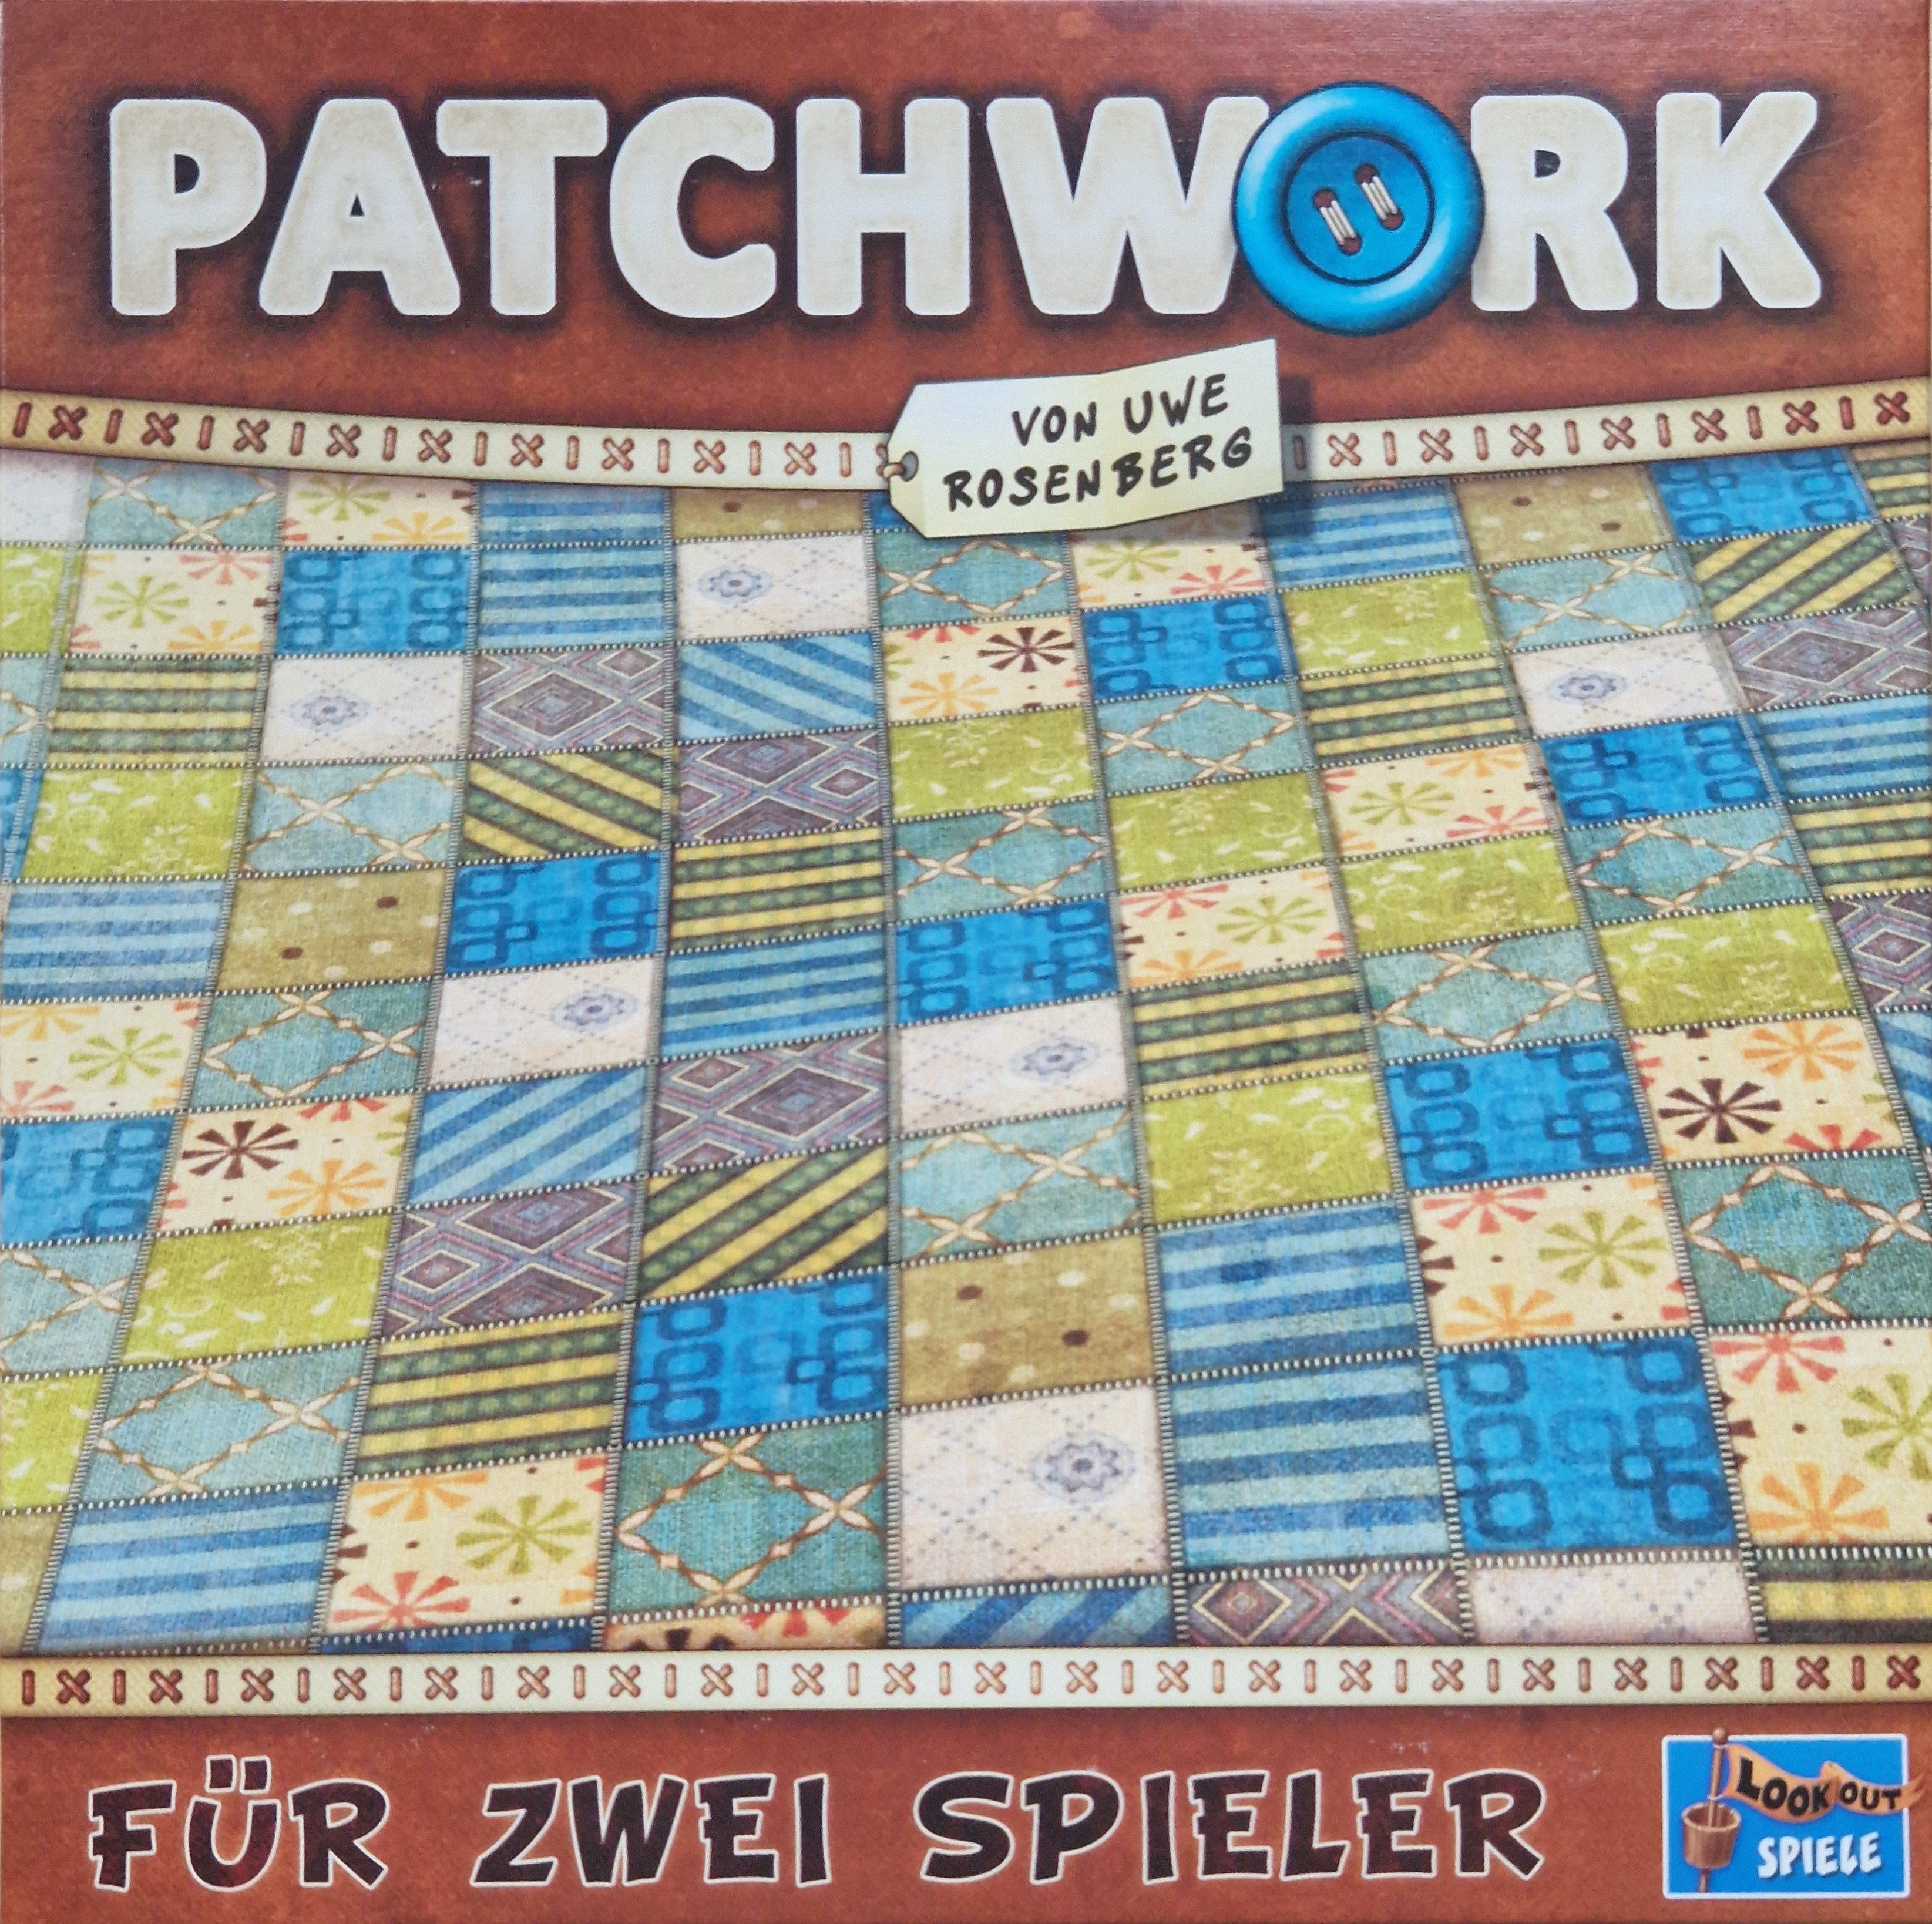
\includegraphics[width=0.28\textwidth]{res/pictures/assets/patchwork-cover.png}
    \caption[Cover von Patchwork]{\unskip}
    Cover von Patchwork
    \label{fig:patchwork-cover}
    \vspace*{-0.75cm}
\end{wrapfigure}

Patchwork ist ein Brettspiel von Uwe Rosenberg, das 2014 bei Lookout Spiele erschienen ist. Bei dem Brettspiel spielen zwei Spieler vom Alter 8 Jahre und aufwärts gegeneinander, wobei ein Spiel in der Regel ungefähr 30 Minuten lang ist \cite{LookoutSpielePatchwork}. Bei dem Brettspiel gestalten zwei Spieler jeweils eine eigne Decke aus Stoffresten, Flicken und Knöpfen, der Technik entsprechend, die der Titel vorgibt. \cite{SpielDesJahresPatchwork}

Das Ziel der Spieler ist mit den gegebenen Stoffplättchen unterschiedlicher Formen und Größen die vorgegebene Fläche zu füllen. Das Puzzlespiel erfordert taktisches Gespür, da die Flickenauswahl die Zugfolge und auch die Flickenauswahl des Gegenspielers beeinflusst. Immer können die Spieler jedoch nicht die gewünschten Flicken verwenden, da diese mit der Spielwährung Knöpfe aus der eigenen Kasse bezahlt werden müssen. An die begehrten Knöpfe kommen die Spieler über die bereits eingearbeiteten Flicken, welche Knöpfe auf sich abgebildet haben. Je mehr dieser Knöpfe auf der eigenen Decke abgebildet sind, desto höher das Einkommen an Knöpfen. Wer am Schluss des Spiels die meisten Knöpfe erwirtschaftet und seine Decke gut bestickt hat, gewinnt den Nähwettstreit. \cite{SpielDesJahresPatchwork}

\section{Spieltheorie}
\label{chapter:spieltheorie}

TODO:

\subsection{Spielbaum}

TODO: Spielbaum, Entscheidungsbaum

\subsection{Spielkomplexität}

TODO:

\begin{itemize}
    \item \textbf{Zustandsraum-Komplexität}: TODO:
    \item \textbf{Spielbaumgröße}: TODO:
    \item \textbf{Entscheidungskomplexität}: TODO: needed?
    \item \textbf{Spielbaumkomplexität}: TODO:
\end{itemize}

\section{Lineare Programmierung}
\label{chapter:lineare-programmierung}

TODO:

\section{Minimax-Algorithmus}
\label{chapter:minimax-algorithmus}

TODO:

Hier haben wir mehr

\section{Monte Carlo Tree Search}
\label{chapter:monte-carlo-tree-search}

\acf{MCTS} ist ein Suchalgorithmus, welcher verwendet wird, um in einem Spiel die beste Aktion zu finden. Dazu wird der Algorithmus während der Entscheidungszeit des Computerspielers ausgeführt. Innerhalb dieser Zeit wird schrittweise ein Suchbaum erstellt. Dabei wird für jede Aktion eine Heuristik erstellt, indem sehr viele Spiele zufällig bis zum Ende ausgespielt werden. Dadurch ergibt sich über die Zeit eine Wahrscheinlichkeit für das Ergebnis des Spiels für jede mögliche Aktion \cite[S. 61]{2008.ParallelMCTS}. Der \ac{MCTS}-Suchprozess besteht aus vier Phasen:

\begin{enumerate}
    \item \textbf{Selektion}: Der Suchbaum wird beginnend ab dem Wurzelknoten bis zu einem Blattknoten durchlaufen, indem in jeder Ebene immer genau ein Kindknoten nach einer bestimmten Richtlinie ausgewählt wird. \cite[S. 187]{2018.ReinforcementLearning}
    \item \textbf{Expansion}: Der ausgewählte Blattknoten wird um ein weiteres Kind erweitert, indem ein noch nicht erforschte Aktion ausgeführt wird. \cite[S. 61]{2008.ParallelMCTS}
    \item \textbf{Simulation}: Ausgehend vom neu hinzugefügten Knoten wird das Spiel bis zum Ende simuliert, indem bis Spielende zufällige Aktionen ausgeführt werden. \cite[S. 61]{2008.ParallelMCTS}
    \item \textbf{Backpropagation}: Das Ergebnis der Simulation wird durch den Suchbaum rückpropagiert, indem das Ergebnis (Gewonnen oder Verloren) ausgehend von dem in Zweitens neu hinzugefügten Knoten bis zum Wurzelknoten hochgereicht wird. \cite[S. 187]{2018.ReinforcementLearning}
\end{enumerate}

Die vier Phasen sind anschaulich in Abbildung \ref{fig:mcts-phases} dargestellt. Diese Phasen werden so lange wiederholt, bis die Entscheidungszeit vorbei ist.

\begin{figure}[!ht]
    \centering
    
\includegraphics[width=\textwidth]{res/pictures/mcts-phases.pdf}
    \caption{Phasen des \acs{MCTS} Algorithmus}
    \label{fig:mcts-phases}
\end{figure}

Für die erste Phase der Selektion wird im Normalfall die in \ref{eqn:uct} dargestellte \ac{UCT} Formel verwendet. Die \ac{UCT} Formel balanciert die Entscheidung zwischen der Ausnutzung von bereits bekannten Aktionen mit der Erkundung von unsicheren Aktionen \cite[S. 206]{2009.ComputerGoMCTS}. Dazu wird im ersten Teil die Anzahl der Siege ($w$) durch die Anzahl der Besuche des Kindknotens ($n$) geteilt. Dieser Term wird immer größer, je öfters eine Simulation nach einem Knotenbesuch gewonnen wird. Der andere Term wird immer größer, je weniger ein Knoten im Vergleich zu seinem Elternknoten ($N$) besucht wird und erzwingt somit auch die Erkundung weniger besuchter Knoten. Bei $c$ handelt es sich um eine Erkundungskonstante, welche das Verhältnis zwischen Ausnutzung und Exploration regelt und normalerweise auf $\sqrt{2}$ gesetzt wird.

\begin{equation}
    \label{eqn:uct}
    \mathbb{U}\mathbb{C}\mathbb{T} = \frac{w}{n} + c \cdot \sqrt{\frac{\ln N}{n}}
\end{equation}

Ein entscheidender Vorteil von \ac{MCTS} ist, dass keine statische Evaluierungsfunktion einer Position wie bei vergleichbaren Algorithmen existieren muss \cite[S. 61]{2008.ParallelMCTS}, da durch zufällige Erkundungen eines Teils des Suchbaums eine Approximation für den tatsächlichen Wert geschaffen wird. \ac{MCTS} hat sich vor allem für Spiele mit einer sehr großen Anzahl an Aktionen bzw. möglichen Zuständen als besser geeignet als traditionelle \hyperref[chapter:minimax-algorithmus]{Minimax}-basierte Programme herausgestellt \cite[S. 1]{2013.MCTSAndMinimaxHybrids} und ist aus diesem Grund auch zu großen Teilen für die Verbesserung der Computergegner in solchen Spielen wie beispielsweise Go verantwortlich \cite[S. 2006]{2009.ComputerGoMCTS} \cite[S. 185]{2018.ReinforcementLearning}.

\section{AlphaZero}
\label{chapter:alphazero}

TODO:

\section{Interaktive Systeme}
\label{chapter:interaktive-systeme}

TODO:


% Deutsche Spielregeln: https://lookout-spiele.de/wp-content/uploads/Patchwork.pdf

\chapter{Analyse des Brettspiels}
\label{chapter:analyse-des-bretspiels}

Im folgenden Abschnitt werden zuerst die Spielregeln von Patchwork genauer erläutert. Darauf aufbauend wird das Spiel nachfolgend mit verschiedenen Ansätzen aus der Spieltheorie analysiert, was später für die Erstellung der unterschiedlichen Computergegner relevant ist.

\section{Spielregeln}
\label{section:spielregeln}

% Terminiologie?
% Patch -> Flick/Flicken
% Button -> Knopf/Knöpfe

Bevor der eigentliche Spielverlauf starten kann, muss das Spiel vorbereitet werden. Hierzu erhalten beide Spieler eine der beiden Decken, auch als Ablageplan bezeichnet, den dazugehörigen Zeitstein und jeweils 5 Knöpfe, welche die Währung im Spiel repräsentieren. Anschließend wird der zentrale Zeitplan in die Mitte des Spielfelds gelegt. Der Zeitplan ist beidseitig mit unterschiedlichen Designs bedruckt, da diese jedoch in allen spielrelevanten Belangen gleich sind, ist die gewählte Seite für den Spielverlauf irrelevant. Die kleinen, braunen Spezialflicken werden jetzt auf den dafür vorgesehenen gedruckten Feldern auf den Zeitplan platziert, welche sich zwischen den Spielfeldern befinden. Nun werden die beiden Zeitsteine der Spieler auf das Startfeld des Zeitplans gestellt. Beginnen darf im Spiel nach dem vollständigen Aufbau des Spielfelds, wer zuletzt eine Nähnadel in der Hand hatte. Daraus ergibt sich, dass bei einem Spiel gegen einen in dieser Arbeit beschriebenen Computergegner, der menschliche Spieler immer mit dem Spiel beginnen muss, da dieser Computergegner noch keine Nähnadeln halten können. Alle Flicken werden nun in einem Kreis oder einer Ellipse um den Zeitplan herum zufällig verteilt und die Spielfigur zwischen dem kleinsten Flicken, der nur zwei Felder auf einem Ablageplan einnimmt, und dem im Uhrzeigersinn folgenden Flicken gesetzt. Die übrig gebliebenen Knöpfe werden zusammen mit dem Sonderplättchen $7\times7$ bereitgelegt. \cite{PatchworkSpielanleitung}

Jetzt kann das Spiel beginnen: Anders als in einem klassischen Spiel sind in diesem Spiel die beiden Spieler nicht unbedingt immer abwechselnd an der Reihe.

TODO:

\section{Spieltheoretische Analyse}

Patchwork ist ein \emph{sequentielles} 2\textendash{}Spieler\textendash{}Brettspiel. Sequentielle Spiele sind rundenbasierte Spiele, bei denen die Spieler nacheinander ziehen \cite[S. 53]{2014.GameTheoryThroughExamples}. Außerdem ist Patchwork ein Spiel mit \emph{perfekter Information}, \dash dass beide Spieler zu jeder Zeit genau wissen, was der andere Spieler getan hat und wie der jetzige Zustand des Spiels ist. Des Weiteren ist Patchwork ein \emph{Strategiespiel}. Wie für viele Strategiespiele typisch, enthält Patchwork auch keinen Zufall während des Spielablaufes. Die einzige Ausnahme ist vor dem Spielbeginn, da dort die Flicken in einer zufälligen Reihenfolge ausgelegt werden. Da beide Spieler in dem Brettspiel versuchen einen Sieg zu erreichen, handelt es sich weiterhin um ein \emph{Nullsummenspiel}. Bei Nullsummenspielen wird der Gewinn für einen Spieler als Verlust des anderen Spielers angesehen. Auch wenn das in Patchwork für einen einzelnen Spielzug nicht unbedingt der Fall sein muss, geht es bei Nullsummenspielen aber nur um das Gewinnen, Verlieren oder Unentschieden des gesamten Spiels.

\subsection*{Anzahl der möglichen Startpositionen}

Das Brettspiel ist bis auf die Startposition der Spielteile deterministisch. Der einzige Zufallsfaktor beim Start ist das Auslegen der einzelnen Flicken im Kreis. Es gibt insgesamt 33 Flicken, welche ausgelegt werden müssen. Jedoch ist der kleinste Flicken, welcher nur 2 Felder auf einem Ablageplan einnimmt ($2\times1$ bzw. $1\times2$), immer an der gleichen Position direkt hinter der Spielfigur. Somit gibt es nur noch 32 Flicken, dessen Positionen angeordnet werden müssen. Eine solche Anordnug aller 32 Flicken auf 32 mögliche Positionen wird als \emph{Permutation} bezeichnet und besitzt $32! = 263.130.836.933.693.530.167.218.012.160.000.000 \approx 2,6 \cdot 10^{35}$ Möglichkeiten. Somit gibt es $2,6 \cdot 10^{35}$ mögliche Startpositionen.

\subsection*{Isomorphie der Zeitpläne}

Wie bereits in »\nameref{section:spielregeln}« erläutert, existieren zwei verschiedene Zeitpläne, welche jedoch nur anders gestaltet sind. Somit sind beide Zeitpläne isomorph zueinander, \dash sie weisen dieselbe Struktur auf, obwohl der konkrete Aufbau verschieden ist. Diese innere Struktur ist zusammen mit den beiden Zeitplänen in \ref{tabelle:isomorphie-zeitplan} veranschaulicht.

\begin{table}[!ht]
    \centering
    \begin{tabular}[t]{cc}
        \adjustbox{center, width=0.35\textwidth, valign=m, margin=0 1ex 0 0}{\begin{tikzpicture}
                                                                                     \node [inner sep=0pt,,outer sep=0pt,clip,rounded corners=0.15cm] (image) at (0,0) {\includegraphics[width=0.75\textwidth]{res/pictures/assets/game_board_side_1.png}};
                                                                                     \drawshadow{image}
                                                                                 \end{tikzpicture}} &
        \adjustbox{center, width=0.35\textwidth, valign=m, margin=0 1ex 0 0}{\begin{tikzpicture}
                                                                                     \node [inner sep=0pt,,outer sep=0pt,clip,rounded corners=0.15cm] (image) at (0,0) {\includegraphics[width=0.75\textwidth]{res/pictures/assets/game_board_side_2.png}};
                                                                                     \drawshadow{image}
                                                                                 \end{tikzpicture}} \\
        \multicolumn{2}{c}{\adjustbox{valign=m, margin=0 2ex 0 2ex}{Zugrundeliegende Struktur des Zeitplans:}}                                                                         \\
        \multicolumn{2}{c}{\adjustbox{width=0.995\textwidth}{
\includegraphics{res/pictures/ZeitplanStruktur.pdf}}}                                                                     \\
    \end{tabular}
    \vspace{5pt}
    \caption{Die Zeitpläne zusammen mit der zugrundeliegenden Struktur}
    \label{tabelle:isomorphie-zeitplan}
\end{table}

Aus diesem Grund kann Patchwork nachfolgend als ein Spiel betrachtet werden, da die Auswahl eines konkreten Zeitplans keinen Unterschied für die Betrachtung ausmacht.

\subsection*{Länge des Spiels}

In der Spieltheorie ist der Begriff eines Spielzuges nicht eindeutig. Ein Spielzug könnte eine einzelne Aktion eines Spielers sein, \zB das Auswählen und Legen eines Flickens in Patchwork von einem Spieler. Jedoch kann ein Spielzug auch so verstanden werden, dass beide Spieler eine Aktion machen müssen. So wird beispielsweise in rundenbasierten Spielen wie Schach ein Spielzug oft so angesehen, dass einmal die weiße und einmal die schwarze Seite gezogen haben müssen. Aufgrund dieser Zweideutigkeit wird ein Spielzug in der Spieltheorie mit einem \hyperref[text:ply]{\emph{Ply}} genauer definiert.

\begin{defStrich}[Ply]
    Ein Spielzug, welcher von einem Spieler gezogen wird, und stellt die kleinste mögliche Aktion in einem Spiel dar. \cite[S. 213]{1959.GameTheoryStudiesCheckers}
\end{defStrich}
\label{text:ply}
\vspace{-0.2cm}

Durch diese Definition kann genau definiert werden, was mögliche \hyperref[text:ply]{\emph{Plys}} in Patchwork sind. Die obige Definition für einen Spielzug, bei dem beide Spieler gezogen haben müssen, ist in Patchwork sowieso schwierig umzusetzen, da ein Spieler mehrere \hyperref[text:ply]{\emph{Plys}} hintereinander ausführen kann. Insgesamt gibt es drei mögliche Arten von \hyperref[text:ply]{\emph{Plys}} in Patchwork:

\begin{itemize}
    \item Vorrücken des Zeitsteins und Knöpfe erhalten
    \item Einen Flicken nehmen und auf der Decke platzieren
    \item Das Legen eines Spezialflicken auf die Decke
\end{itemize}

Immer wenn ein Spieler an der Reihe ist, kann er zwischen dem Vorrücken und dem Platzieren von drei Flicken unterscheiden. Die Aktion einen Spezialflicken auf die Decke zu legen, kommt im Spiel immer genau fünfmal vor.

Patchwork endet, sobald beide Zeitsteine der Spieler das Zielfeld auf der Zeitleiste erreicht haben. Um ein möglichst langes Spiel zu spielen, muss also die Anzahl der Felder, die ein Spieler mit seinem Zeitstein pro \hyperref[text:ply]{\emph{Ply}} vorzieht, minimiert werden.

Für die Aktion \enquote{Einen Flicken nehmen und auf der Decke platzieren} ist die Anzahl der Felder immer durch den ausgewählten Flicken vorgegeben und beträgt mindestens 1 und maximal 6.

Die Anzahl der Felder bei der Aktion \enquote{Vorrücken des Zeitsteins und Knöpfe erhalten} ist abhängig von der relativen Position der einzelnen Zeitsteine zueinander. Die maximale Anzahl an Feldern, die ein Zeitstein in einem Zug vorrücken kann, beträgt 7. Da immer ein Spielerwechsel stattfindet, sobald der Zeitstein des derzeitigen Spielers weiter vorrangeschritten ist als der Zeitstein des Gegners, muss für eine maximale Anzahl die Distanz zwischen den Zeitsteinen möglichst groß sein. Ein Zeitstein kann sich von dem anderem Zeitstein nur um maximal 6 Felder entfernen. Das ist der Fall, wenn der Flicken mit Zeitkosten 6 ausgewählt wird, während sich beide Zeitsteine auf demselben Feld befinden. Nach dieser Aktion ist der andere Spieler an der Reihe, welche sein Zeitstein um 7 Felder fortbewegen kann (Distanz von 6 Feldern $+$ 1 Feld, um weiter vorrangeschritten zu sein als der andere Zeitstein). Die minimale Anzahl an Felder bei der Vorrücken-Aktion beträgt 1 und kann bei drei Spielzuständen auftreten. Zuerst ist es möglich, dass beide Zeitsteine auf demselben Feld sind, sodass der Spieler, welcher an der Reihe ist, seinen Zeitstein nur 1 Feld vorrückt. Weiterhin ist es möglich, dass ein Zeitstein auf dem Feld vor dem Ziel ist, während der andere Spieler bereits im Ziel ist. In dieser Situation darf der Zeitstein auch nur um ein Feld vorgerückt werden. Zuletzt existiert noch die Situation am Spielanfang. Da hier auch beide Zeitsteine auf demselben Feld \textemdash{} dem Startfeld des Zeitplans \textemdash{} sind, darf der Startspieler den Zeitstein auch nur um ein Feld vorrücken.

Um die Länge des Spiels zu maximieren, sollte jeder Spieler so wenige Felder wie möglich vorrücken. Nutzt jeder Spieler immer die \enquote{Vorrücken des Zeitsteins und Knöpfe erhalten} Aktion, so gibt es insgesamt 54 \hyperref[text:ply]{\emph{Plys}}, da auf dem Zeitplan insgesamt 53 Felder sowie ein Start- und ein Zielfeld existieren. Während beim ersten und letzen \hyperref[text:ply]{\emph{Ply}} der Erste bzw. Zweite Spieler seinen Zeitstein nur um 1 Feld vorrückt, muss der Zeitstein während des Spiels immer 2 Felder vorgerückt werden, da die vorherige Aktion \textemdash{} auch eine \enquote{Vorrücken des Zeitsteins und Knöpfe erhalten} Aktion \textemdash{} impliziert, dass der Zeitstein des Gegners genau 1 Feld vor dem eigenen Zeitstein liegt.

\begin{table}[!ht]
    \centering
    \resizebox{\textwidth}{!}{
        \begin{tabular}[t]{c|c|c|c}
            \adjustbox{valign=t, raise=-16.25ex}{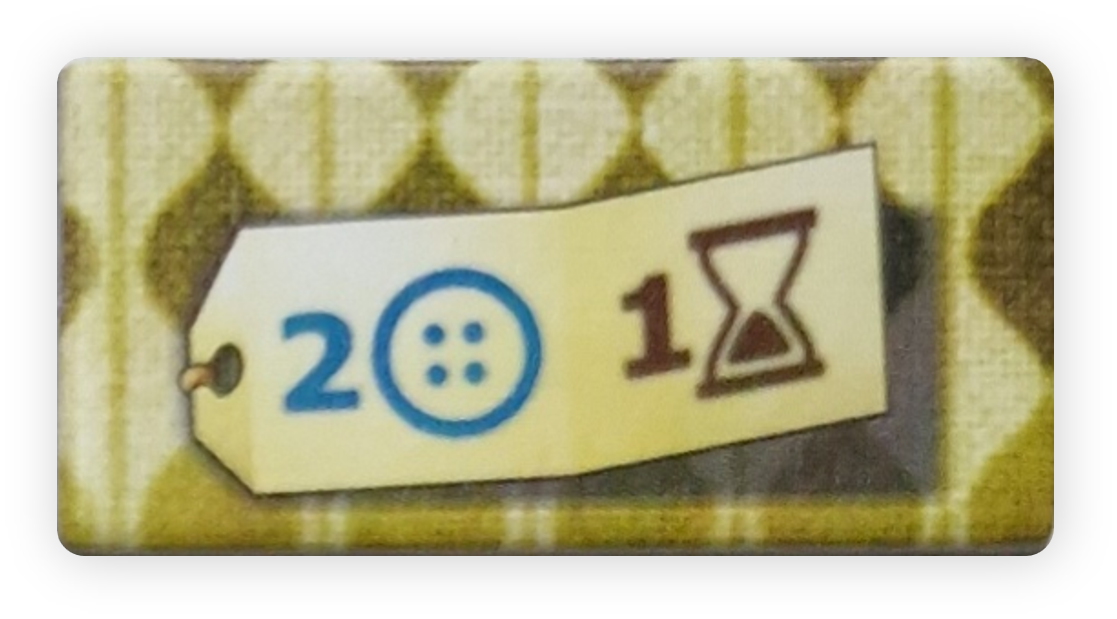
\includegraphics[width=0.2\textwidth]{res/pictures/assets/00_front.png}} &
            \adjustbox{valign=t, raise=0ex}{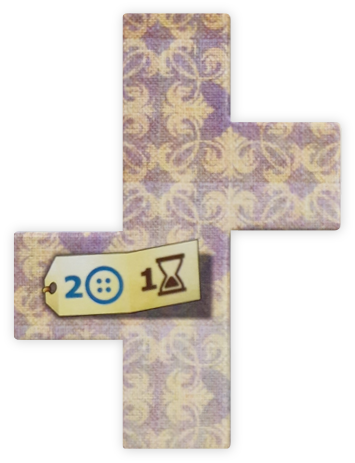
\includegraphics[width=0.3\textwidth]{res/pictures/assets/06_front.png}}      &
            \adjustbox{valign=t, raise=-9.05ex}{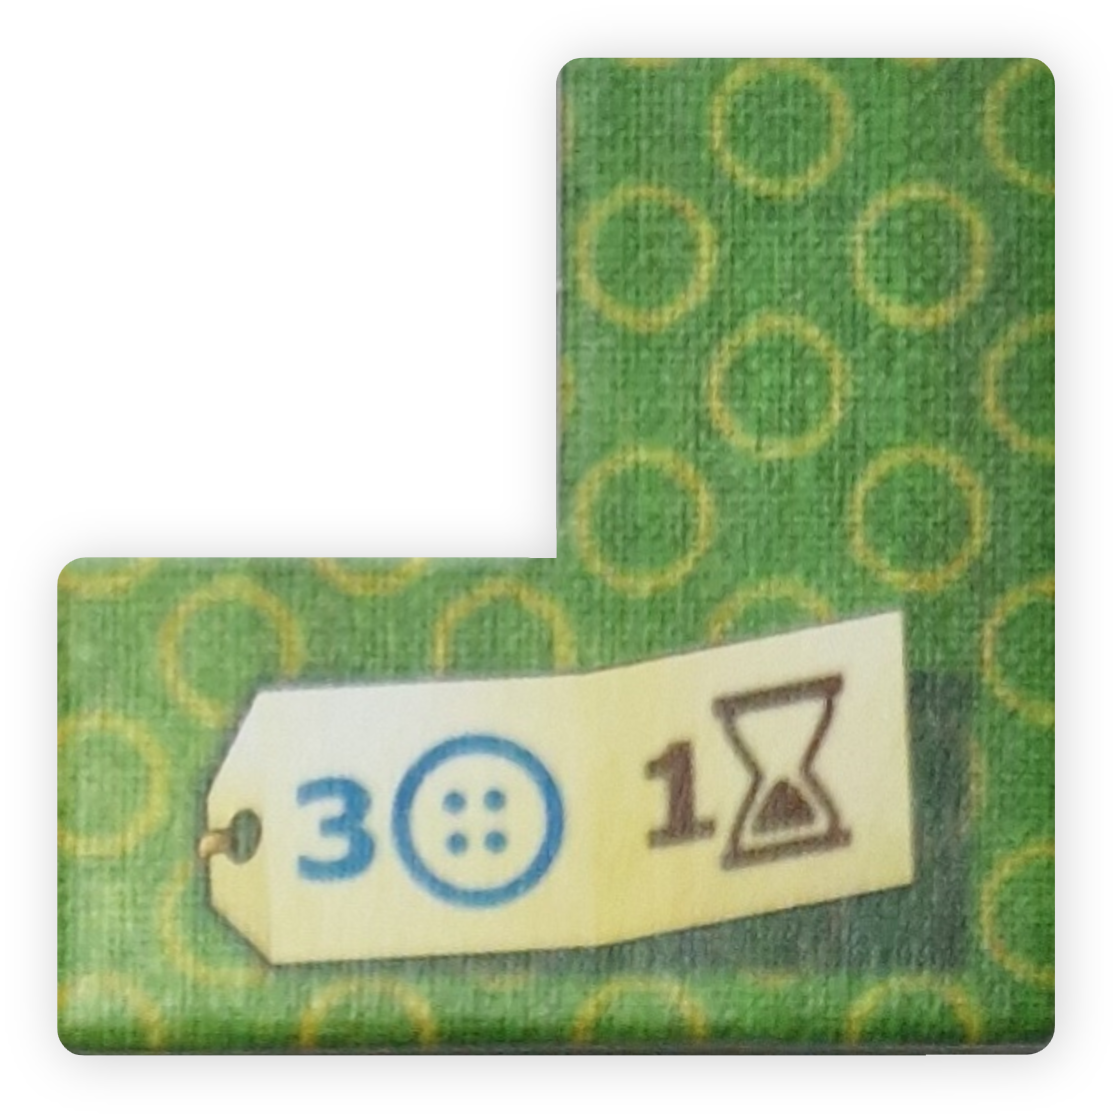
\includegraphics[width=0.2\textwidth]{res/pictures/assets/21_front.png}}  &
            \adjustbox{valign=t, raise=-16.25ex}{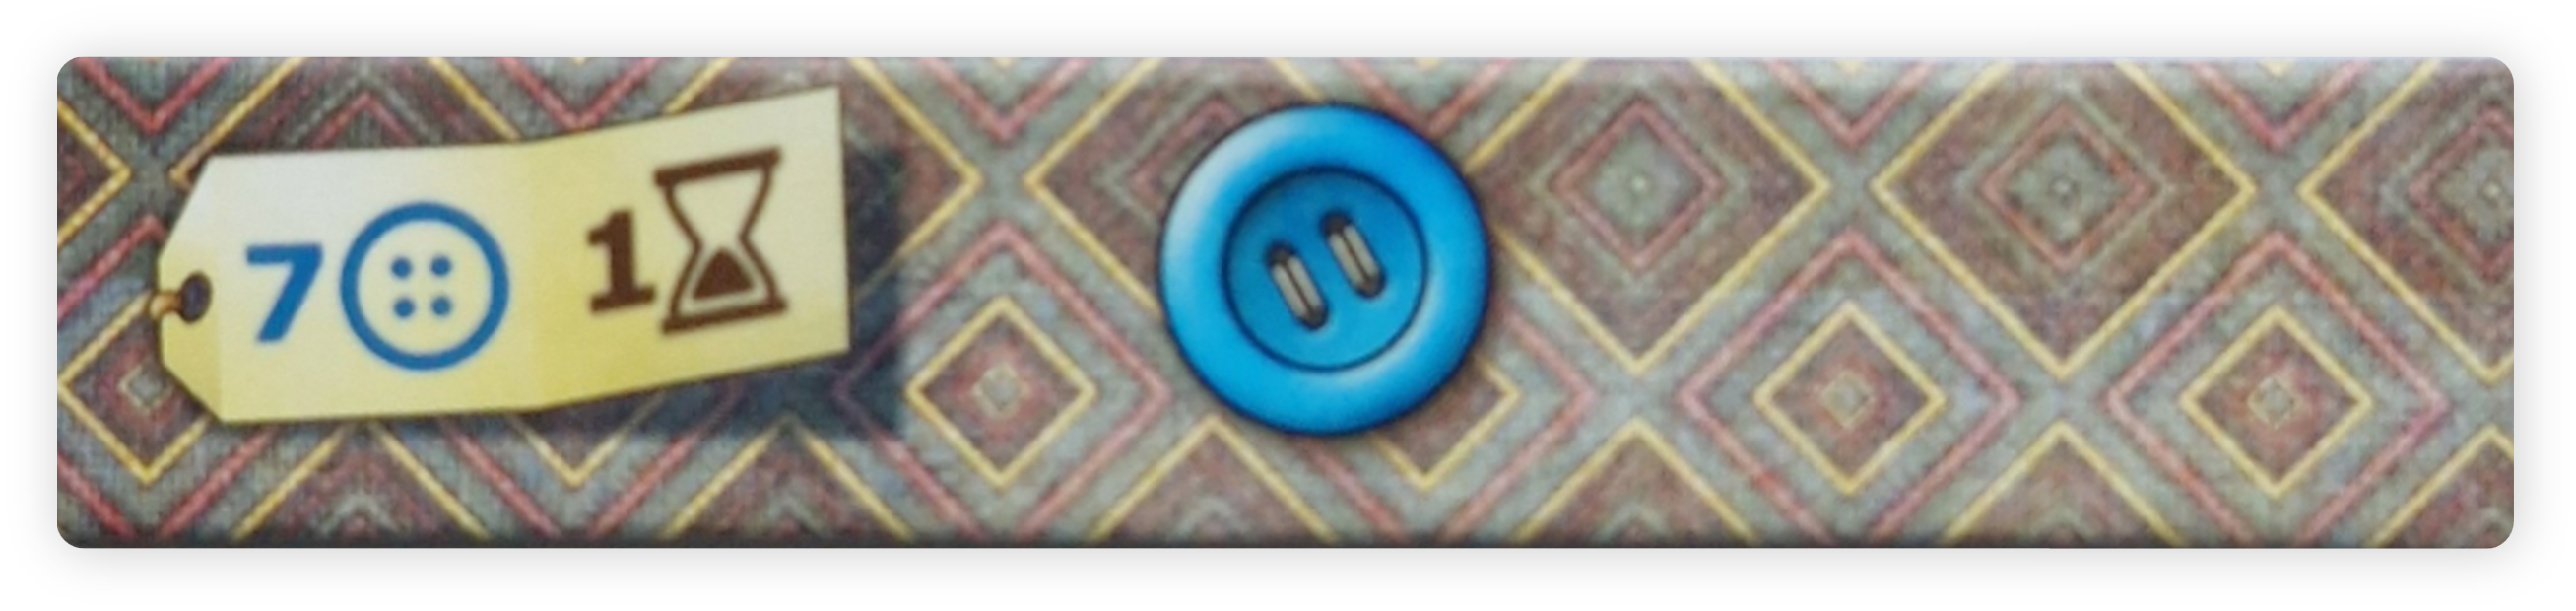
\includegraphics[width=0.5\textwidth]{res/pictures/assets/27_front.png}}   \\
        \end{tabular}
    }
    \vspace{5pt}
    \caption{Die vier Flicken mit Zeitkosten 1}
    \label{tabelle:flicken-mit-zeitkosten-1}
\end{table}

Die Zeitkosten bei der Aktion \enquote{Einen Flicken nehmen und auf der Decke platzieren} sind immer fest, wobei es insgesamt neun Flicken gibt, bei denen die Zeitkosten auch 2 betragen. So können optimal 9 Vorrücken-Aktionen durch die Auswahl dieser Flicken ersetzt werden. Weiterhin gibt es aber auch noch die vier in \ref{tabelle:flicken-mit-zeitkosten-1} dargestellten Flicken, welche nur Zeitkosten von 1 besitzen. Wird nun ein Vorrücken-\hyperref[text:ply]{\emph{Ply}} mit 2 Zeitkosten durch eine Kombination aus Flicken mit Zeitkosten 1 auswählen und auf der Decke Platzieren und anschließend ein Vorrücken-\hyperref[text:ply]{\emph{Ply}} mit Zeitkosten 1 ersetzt, ist das Spiel um 4 weitere \hyperref[text:ply]{\emph{Plys}} verlängert. Das ist möglich, da davon wie oben beschrieben der Zeitstein des derzeitigen Spielers immer direkt hinter dem Zeitstein des Gegners ist. Wird nun ein Flicken mit Zeitkosten 1 ausgewählt, befindet sich der Zeitstein des derzeitigen Spielers auf dem Zeitstein des Gegners. So kann ein Vorrücken-\hyperref[text:ply]{\emph{Ply}} mit Zeitkosten von 1 anstatt 2 ausgeführt werden. Da alle anderen Flicken höhere Zeitkosten verlangen, ist keine weitere Optimierung des Spiels hinsichtlich der der maximalen Länge mehr möglich.

Die maximale Länge des Brettspiels ergibt sich somit aus der Kombination der 54 Vorrücken-\hyperref[text:ply]{\emph{Plys}} zusammen mit den 4 zusätzlich gewonnenen \hyperref[text:ply]{\emph{Plys}} durch das Legen von Flicken mit Zeitkosten 1. Weiterhin kommen noch die fünf \hyperref[text:ply]{\emph{Plys}} für das Legen von Spezialflicken hinzu. Somit beträgt die maximale Länge von Patchwork \textbf{63} \hyperref[text:ply]{\emph{Plys}}.

\subsection*{Obere Schranke für die maximal mögliche Anzahl an Aktionen in einem \hyperref[text:ply]{Ply}}

\textbf{Supremum/Maximum für die maximal mögliche Anzahl an Aktionen in eimem Ply}

bla bla mit Spiegelungen und Rotationen (Diedergruppe der Ordnung 4 vgl. $D_4$-Gruppe)


tatsächlicher Wert

% #
% #  gibt es in der Form 2 mal --> 8*7*8 = 448
% ##

% #
% ## --> 8*7*8 = 448
% ##

% 3*448=1344

% nicht verwendet

% ##
% ##  --> 7*7*8=392 (kostet aber 8 somit nicht möglich)
% ##

% #
% ## --> 8*8*4 = 256

% ## --> 8*9*2 = 144

% #  --> 9*9*1 = 81


$\left(9-\text{Breite}+1\right)\cdot\left(9-\text{Länge}+1\right)\cdot\text{Transformationen}$

bei flicke der breite ... und länge ... kann man es auf ... positionen im board legen

max amount of moves
* upper bound
* real value

\subsection*{Obere und untere Schranke für die Wertung eines Spielers}

In dieser Sektion wird eine obere und eine untere Schranke für die Wertung eines Spielers am Ende des Spiels festgesetzt. Da sich die Wertung aus dem am Ende vorhandenen Vorrat an Knopf-Plättchen und der Anzahl der Lücken im eigenen Spielbrett zusammensetzt, werden zunächst die maximal möglichen Werte für diese beiden Komponenten bestimmt. Anschließend werden die Schranken für die Wertung eines Spielers am Ende des Spiels festgesetzt.

\subsection*{Maximal mögliche Anzahl zusätzlichen Knopf-Plättchen an bei der Knopf-Wertung}

TODO:

Max Button Income
% /// The maximum amount of button income a player can have is bounded
% /// by the number of tiles in the quilt board.
% ///
% /// The highest possible upper bound that is realistic would therefore be `81`
% /// (The amount of tiles in the quilt board). But this would require that
% /// all patches that are layed out have at least the same button income as
% /// the amount of tiles they cover. This is not true for any patch in the
% /// game.
% ///
% /// Therefore variable uses a more conservative upper bound of `32`.
% /// For this the patches were ordered by the percentage of button income in
% /// relation to the amount of tiles they cover. Then the first patches were
% /// chosen until the amount of tiles covered was `>= 81`. With this a
% /// maximum button income of 33 as upper bound was found.
% ///
% /// Here is the list of all patches and the patches that were chosen ordered
% /// by the percentage of button income in relation to the amount of tiles:
% ///
% /// ```txt
% /// index:  4, tiles: 4, buttons: 3, percentage: 0.75
% /// index:  1, tiles: 5, buttons: 3, percentage: 0.6
% /// index:  3, tiles: 6, buttons: 3, percentage: 0.5
% /// index:  9, tiles: 4, buttons: 2, percentage: 0.5
% /// index: 12, tiles: 6, buttons: 3, percentage: 0.5
% /// index: 14, tiles: 4, buttons: 2, percentage: 0.5
% /// index: 17, tiles: 5, buttons: 2, percentage: 0.4
% /// index: 18, tiles: 5, buttons: 2, percentage: 0.4
% /// index: 29, tiles: 5, buttons: 2, percentage: 0.4
% /// index: 13, tiles: 6, buttons: 2, percentage: 0.3333333333333333
% /// index: 15, tiles: 6, buttons: 2, percentage: 0.3333333333333333
% /// index: 30, tiles: 6, buttons: 2, percentage: 0.3333333333333333
% /// index: 19, tiles: 4, buttons: 1, percentage: 0.25
% /// index: 26, tiles: 4, buttons: 1, percentage: 0.25
% /// index: 28, tiles: 4, buttons: 1, percentage: 0.25
% /// index: 10, tiles: 5, buttons: 1, percentage: 0.2
% /// index: 27, tiles: 5, buttons: 1, percentage: 0.2
% /// --------------- CUTOFF AFTER 84 >= 81 TILES COVERED ---------------
% /// index: 31, tiles: 5, buttons: 1, percentage: 0.2
% /// index: 16, tiles: 6, buttons: 1, percentage: 0.16666666666666666
% /// index: 32, tiles: 6, buttons: 1, percentage: 0.16666666666666666
% /// index: 20, tiles: 7, buttons: 1, percentage: 0.14285714285714285
% /// index:  2, tiles: 8, buttons: 1, percentage: 0.125
% /// index:  0, tiles: 2, buttons: 0, percentage: 0
% /// index:  5, tiles: 6, buttons: 0, percentage: 0
% /// index:  6, tiles: 6, buttons: 0, percentage: 0
% /// index:  7, tiles: 7, buttons: 0, percentage: 0
% /// index:  8, tiles: 5, buttons: 0, percentage: 0
% /// index: 11, tiles: 6, buttons: 0, percentage: 0
% /// index: 21, tiles: 3, buttons: 0, percentage: 0
% /// index: 22, tiles: 5, buttons: 0, percentage: 0
% /// index: 23, tiles: 3, buttons: 0, percentage: 0
% /// index: 24, tiles: 4, buttons: 0, percentage: 0
% /// index: 25, tiles: 3, buttons: 0, percentage: 0
% /// ```
% ///
% /// But this is not the least upper bound (supremum) as the tiles covered
% /// are `84` in the end and not `81`. The actual supremum is a button
% /// income of `32`. This is the case because the most one can cover below
% /// the limit of 81 tiles is reached is only a button income of `32`.
% /// Then at least 79 tiles are covered and all patches with 2 tiles or less
% /// do not have any button income. To show that this is actually not only
% /// the supremum but a reachable maximum a quilt board has to be constructed
% /// that has a button income of 32. This is done in the following:
% ///
% /// ```txt
% /// 28 28 28 28 10 10 10 XX 13
% /// 19 19 19 10 10 13 13 13 13
% /// 19 04 18 18 18 18 12 12 13
% /// 04 04 18 XX 12 12 12 12 14
% /// 04 30 29 29 29 17 14 14 14
% /// 30 30 30 29 17 17 17 03 03
% /// 30 26 30 29 01 17 03 03 03
% /// 26 26 15 15 01 01 03 09 09
% /// 26 15 15 15 15 01 01 09 09
% ///
% /// where the tiles covered with XX are still free and all the other tiles
% /// have the id of the patch that covers them.
% /// ```
% ///
% /// This quilt board has a button income of 32, has a time cost of 66 and
% /// covers at least 79 tiles but can be filled up with two special patches
% /// to cover the full quilt board. While this is a maximum that can be
% /// created on the quilt board, it is not achievable in the game as the
% /// time cost of 66 is greater than the allowed time cost of 54.
% ///
% /// TODO: improve the bound even more
% ///

\subsection*{Maximal mögliche Anzahl an Knopf-Plättchen}


Bounds for lowest possible score, highest possible score, max button income, max button balance

Max button balance
TODO: take update from zobrist hash in rust implementation
% /// The maximum button balance a player can have is bounded by the game.
% ///
% /// * A player has `5` buttons at the start of the game.
% /// * There are only `9` button income triggers that can yield a maximum amount
% ///   of `33` buttons each (see `MAX_BUTTON_INCOME` estimate below).
% /// * The player can get `1` button income for every tile he walks on the
% ///   time track with the walking action. There are `54` tiles on the time track.
% /// * The only other income source are the `7` buttons from a full quilt board.
% ///
% /// Because of this the maximum button balance a player can have is bounded
% /// by `5 + 9 · 33 + 7 + 54 · 1 = 363`. This is a upper bound and not the
% /// actual maximum because of the same reason as the `MAX_BUTTON_INCOME`
% /// estimate below. Furthermore the player can only choose between the
% /// walking action and the action to place a tile. Therefore he cannot get
% /// both at the same time. It would probably be possible to lower the bound
% /// to `5 + 9 · 33 + 7 + 54 · 1 = 309` (remove the walking actions) and
% /// still be correct. But to be safe the bound is kept at `363`.


MAX possible score
363 = same as max button balance

min score
0 als bound für income + -81*2 als Punkte am Ende

-81*2 + 0 = -162

nicht realistisch, da man immer durch laufen mindestens 1 punkte bekommt. einzige möglichkeit punkte loszuwerden ist das quilt board zu füllen
\chapter{Modellierung von Patchwork als Computerprogramm}
\label{chapter:modellierung-von-patchwork-als-computerprogramm}

TODO: Erst generelle Architektur, Programmiersprache usw. hier auch generelle speicherung (spieler, Sonderplättchen, zeitplan, ...)

\begin{itemize}
    \item Aufbau des Spielfeldes
    \item Speicherung der Quilt Boards (Row-Major)
    \item Speicherung des Time Boards
    \item Speicherung der Patchliste
    \item Umsetzung von Zügen
    \item Effizienzoptimierungen (u128, vorberechnete Transformationen, ...)
    \item Abstraction von Player Interface
    \item Evaluator, Move Orderer, Tree Policy (wahrscheinlich später)
\end{itemize}

TODO: Zeitplan einfaches Array mit Bitflags

Besondere extra:

\section{Aufbau des Ablageplans}

\lstinputlisting[
    label={code:quilt-board-definition},
    caption={Definition der QuiltBoard-Struktur},
    captionpos=b,
    language=Rust,
    firstline=0,
]{res/code/quilt-board-definition.rs}

Der Ablageplan eines Spielers wird durch die in Quellcode \ref{code:quilt-board-definition} definierte Struktur \code{QuiltBoard} modelliert. Dabei existieren nur 2 Attribute. Zuerst wird das Knopfeinkommen mit \code{button\_income} gespeichert, was durch die auf dem Ablageplan liegenden Flicken beim Passieren einer Knopf-Wertung generiert wird. Das zweite Attribut \code{tiles} dient dazu, den Status der einzelnen Felder auf dem Ablageplan zu speichern. Der Ablageplan besteht aus 81 Feldern, die in 9 Zeilen und 9 Spalten angeordnet sind, und für die jeweils gespeichert werden muss, ob das Feld belegt ist oder nicht. Da alle Abfragen bezüglich Status der Felder so schnell wie möglich sein sollen, kommt hier anstatt eines üblichen 2-dimensionalen Arrays eine \ac{u128} zum Einsatz. Da nur zwei Zustände existieren, kann für jedes Feld ein Bit verwendet werden. Weiterhin werden alle Felder des Ablageplans zeilenweise wie in Abbildung \ref{fig:quilt-board-storage} in einer Ganzzahl nacheinander abgelegt.

\begin{figure}[!ht]
    \centering
    \rlap{{\color{white}\acf{LSB} \acf{MSB}}} \vspace*{-\baselineskip}
    \includegraphics[width=\textwidth]{res/pictures/quilt-board-storage.pdf}
    \caption{Zeilenweise Anordnung der Felder des Ablageplans}
    \label{fig:quilt-board-storage}
\end{figure}

Da der Ablageplan 81 Felder umfasst, muss $2^7=128$ Bit als Ganzzahldatentyp verwendet werden. Dieser wird von Rust nativ unterstützt und für 64 Bit Rechner in mehrere Operationen kompiliert. Die oberen Bits der Zahl sind dabei immer auf 0 gesetzt. Durch die effiziente Speicherung des Ablageplans in einem \ac{u128}, können Abfragen bezüglich Befüllung oder Überlagerung von Feldern in konstanter Zeit durch Bitmasken und Bitoperationen durchgeführt werden. Als Beispiel lässt sich hier die Methode zum Überprüfen der notwendigen Bedingung zur Erhaltung des $7\times 7$ Sonderplättchen anführen (Anhang \ref{code:quilt-board-special-tile-condition}).

Besonders anzumerken ist, dass die Flicken und ihre Transformationen, wie sie auf dem Ablageplan liegen, nicht gespeichert werden. Da einige Computergegner wie beispielsweise der \ac{MCTS}-Spieler den Spielstand sehr oft kopieren müssen und die genaue Position der Flicken für die Generierung und Ausführung von Aktionen nicht benötigt wird, würde diese Extrainformation nur zu unnötig erhöhtem Speicherverbrauch führen.

\section{Modellierung der Aktionen}

TODO: Action, ActionId/SurrogateActionId, NaturalActionId

\lstinputlisting[
    label={code:action},
    caption={Definition des Tagged-Union \code{Action}},
    captionpos=b,
    language=Rust,
    firstline=0,
]{res/code/action.rs}

\begin{itemize}
    \item \code{Action} als Tagged-Union
    \item \code{ActionId} bzw. \code{SurrogateActionId} als \ac{u32}
    \item \code{NaturalActionId} als TODO: 2028
\end{itemize}

\section{Flicken und Zugmöglichkeiten}

\acs{u128}

\pagebreak

\begin{table}[H]
    \centering
    \resizebox{\textwidth}{!}{\begin{tabular}{|l|r|c|l|}
            \hline
            \multicolumn{1}{|c|}{Methode}                                                 & \multicolumn{1}{|c|}{Zeit}      & $\mathcal{O}$-Kalkül        & \multicolumn{1}{|c|}{Bemerkungen}                  \\ \hline
            \code{game.get\_initial\_state}                                               & $472{,}11\,\acs{ns}$            & $\mathcal{O}\left(n\right)$ & $n$ aufgrund Mischen der Flicken                   \\  \hline
            \code{game.get\_valid\_actions}                                               & $8{,}91\,\acs{us}$              & $\mathcal{O}\left(n\right)$ & $3\times$Aufruf von Ablageplan Aktionen generieren \\  \hline
            \code{game.get\_random\_action}                                               & $9{,}22\,\acs{us}$              & $\mathcal{O}\left(n\right)$ & Aufruf von \code{get\_valid\_actions}              \\  \hline
            \code{game.do\_action}                                                        & $280{,}00\,\acs{ns}$            & $\mathcal{O}\left(1\right)$ &                                                    \\  \hline
            \code{game.undo\_action}                                                      & $286{,}78\,\acs{ns}$            & $\mathcal{O}\left(1\right)$ &                                                    \\  \hline
            \code{game.clone}                                                             & $1{,}36\,\acs{us}$              & $\mathcal{O}\left(1\right)$ & $\hat{=}$ \code{memcpy}                            \\  \hline
            \code{game.is\_terminated}                                                    & $84{,}79\,\acs{ns}$             & $\mathcal{O}\left(1\right)$ &                                                    \\  \hline
            {\footnotesize \code{action\_id.from\_natural\_action\_id} }                  & $42{,}44\,\acs{ns}$             & $\mathcal{O}\left(1\right)$ &                                                    \\  \hline
            {\footnotesize \code{natural\_action\_id.from\_surrogate\_action\_id} }       & $45{,}97\,\acs{ns}$             & $\mathcal{O}\left(1\right)$ &                                                    \\  \hline
            \code{patch\_manager.get\_patch}                                              & $1{,}87\,\acs{ns}$              & $\mathcal{O}\left(1\right)$ &                                                    \\  \hline
            \code{patch\_manager.get\_special\_patch}                                     & $3{,}70\,\acs{ns}$              & $\mathcal{O}\left(1\right)$ &                                                    \\  \hline
            \code{patch\_manager.get\_transformation}                                     & $2{,}57\,\acs{ns}$              & $\mathcal{O}\left(1\right)$ &                                                    \\  \hline
            \code{player.get\_position}                                                   & $41{,}93\,\acs{ns}$             & $\mathcal{O}\left(1\right)$ &                                                    \\  \hline
            \code{quilt\_board.is\_full}                                                  & $561{,}16\,\acs{ps}$            & $\mathcal{O}\left(1\right)$ &                                                    \\  \hline
            {\footnotesize \code{quilt\_board.is\_special\_tile\_condition\_reached} }    & $523{,}76\,\acs{ps}$            & $\mathcal{O}\left(1\right)$ &                                                    \\  \hline
            \code{quilt\_board.do\_action}                                                & $46{,}90\,\acs{ns}$             & $\mathcal{O}\left(1\right)$ &                                                    \\  \hline
            \code{quilt\_board.undo\_action}                                              & $47{,}18\,\acs{ns}$             & $\mathcal{O}\left(1\right)$ &                                                    \\  \hline
            {\footnotesize \code{quilt\_board.get\_valid\_actions\_for\_patch} }          & $1{,}27\,\acs{us}$              & $\mathcal{O}\left(n\right)$ &                                                    \\  \hline
            {\footnotesize \code{quilt\_board.get\_valid\_actions\_for\_special\_patch} } & $855{,}98\,\acs{ns}$            & $\mathcal{O}\left(n\right)$ &                                                    \\  \hline
            Getter\textendash{} und Setter\textendash{}Methoden                           & \multicolumn{1}{|c|}{$\diagup$} & $\mathcal{O}\left(1\right)$ &                                                    \\  \hline
        \end{tabular}}
    \vspace{3pt}
    \caption{Übersicht über die verfügbaren Methoden in der Patchwork\textendash{}Implementierung}
    \label{tabelle:patchwork-methods}
\end{table}

TODO: Hier fehlt noch der Anhang + Verweis für Benchmark
\chapter{Erstellung der Computerspielengines}
\label{chapter:erstellung-der-computerspielengines}

Nachdem Patchwork auf unterschiedlichste Aspekte analysiert und das Brettspiel als Computerprogramm umgesetzt wurde, werden nachfolgend die verschiedenen Computerspielengines für das Spiel implementiert.

\section{Ansatz A: Zufallsauswahl der Spielzüge}
\label{section:erstellung-ansatz-a}

Um eine Computerspielengine zu erstellen, muss das Trait \code{Player}, welcher in Codeausschnitt \ref{code:player-trait} zu sehen ist, von der Engine implementiert werden. Dafür müssen die zwei Methoden \code{name()} und \code{get\_action()}. Die erste Methode gibt den Namen der Computerspielengine zurück, um sie während des Spiels identifizieren zu können, während die zweite Methode die Aktion als \code{PlayerResult<Action>} zurückgibt, die der Spieler machen möchte und benötigt als Eingabe den aktuellen Zustand des Spiels.

\lstinputlisting[
    label={code:player-trait},
    caption={Definition des Player-Traits},
    captionpos=b,
    language=Rust,
    firstline=0,
]{res/code/player-trait.rs}

Die einfachste Computerspielengine ist der \code{RandomPlayer}, in Codeauschnitt \ref{code:random-player} zu sehen, welcher einen Spieler repräsentiert, der zufällige Züge macht. Zur Auswahl der Züge verwendet die Engine den Zufallsgenerator Xoshiro256++, der einen der möglichen Spielzüge im aktuellen Spielzustand \code{game} auswählt, die durch den Aufruf der Methode \code{game.get\_valid\_actions()} bereitgestellt werden. Diese Computergegner ist gut für Vergleichszwecke im späteren Kapitel \nameref{chapter:evaluation} geeignet, da die zufälligen Züge eine Baseline gegen die komplexeren, strategischen Entscheidungen der anderen Computerspielengines bildet.

\lstinputlisting[
    label={code:random-player},
    caption={Definition des RandomPlayers},
    captionpos=b,
    language=Rust,
    firstline=0,
]{res/code/random-player.rs}

\section{Ansatz B: Greedy-Algorithmus}

TODO: auch Evaluator

\section{Ansatz C: Principal-Variation-Search}
\label{section:erstellung-ansatz-b}

\ac{PV}

Verwendung von Negamax Algorithmus (hier phantom moves) (aufruf mit -)
Erweiterung des Alpha-Beta (ref) Generelle struktur Principal Variation search
Iterative Deepening

\ac{PVS}

\subsection{Aktionen-Anordnung}

TODO:
\cite{2022.MoveOrdering}
Anordnung nicht Sortieren -> Warum überhaupt anordnen und warum nicht sortieren?
-> insertion sort??
Wie gemacht? -> Table mit linearer Interpolation based timeboard position
heatmap generierung erläutern
heatmaps erläutern und warum sinnvoll erscheint
müsste eigentlich symmetrisch sein

\begin{figure}[!ht]
    \centering
    \begin{minipage}{.11\textwidth}
        \centering
        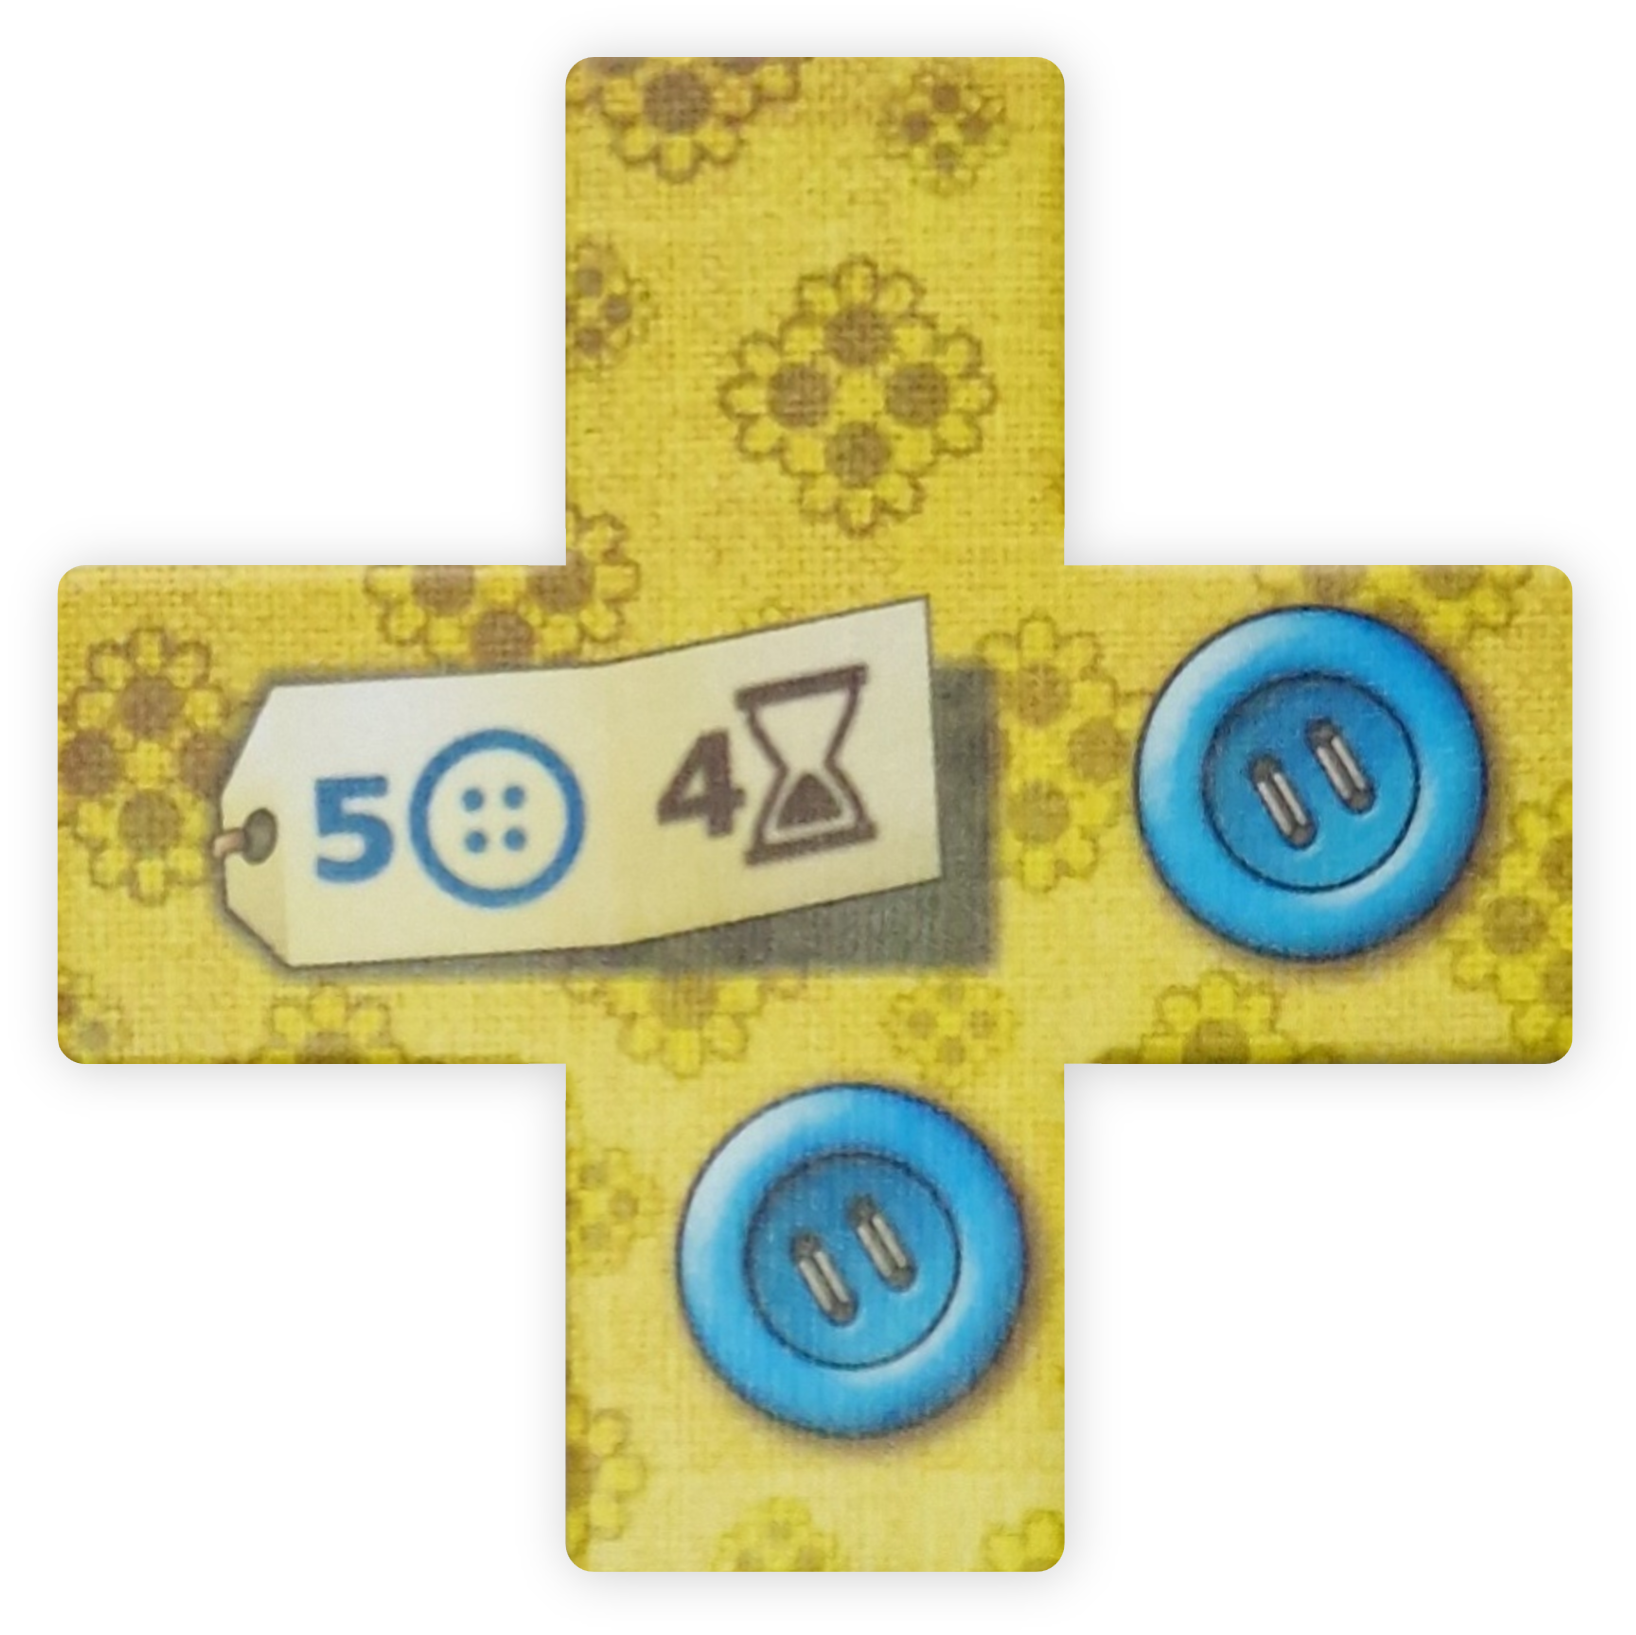
\includegraphics[width=\linewidth]{res/pictures/assets/17-front.png}
    \end{minipage}
    \begin{minipage}{.78\textwidth}
        \centering
        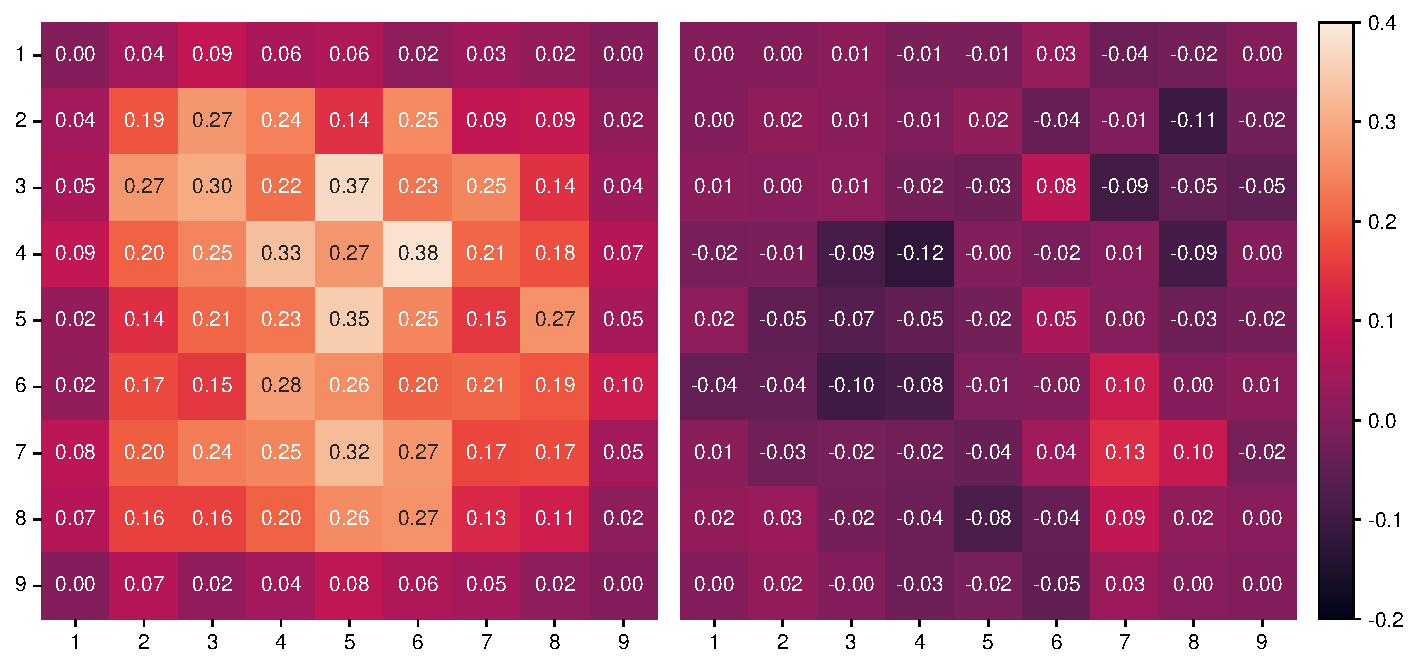
\includegraphics[width=\linewidth]{res/pictures/plots/17-action-ordering.pdf}
    \end{minipage}
    \begin{minipage}{.11\textwidth}
        \hfill
    \end{minipage}
    \captionof{figure}{Heatmap des Flicken 17}
    \label{fig:action-ordering-patch-17}
\end{figure}

\begin{figure}[!ht]
    \centering
    \begin{minipage}{.11\textwidth}
        \centering
        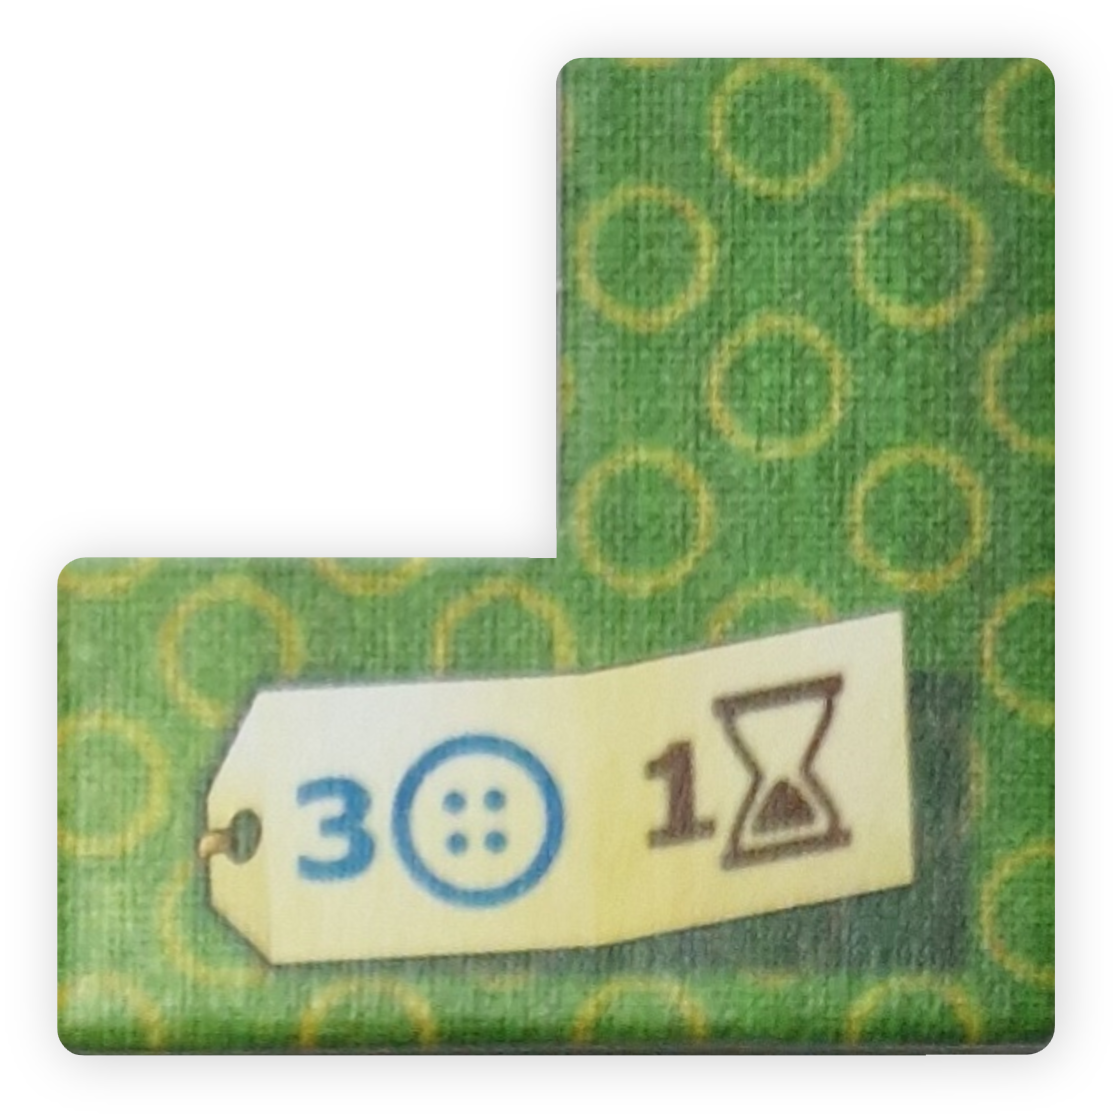
\includegraphics[width=0.667\linewidth]{res/pictures/assets/21-front.png}
    \end{minipage}
    \begin{minipage}{.78\textwidth}
        \centering
        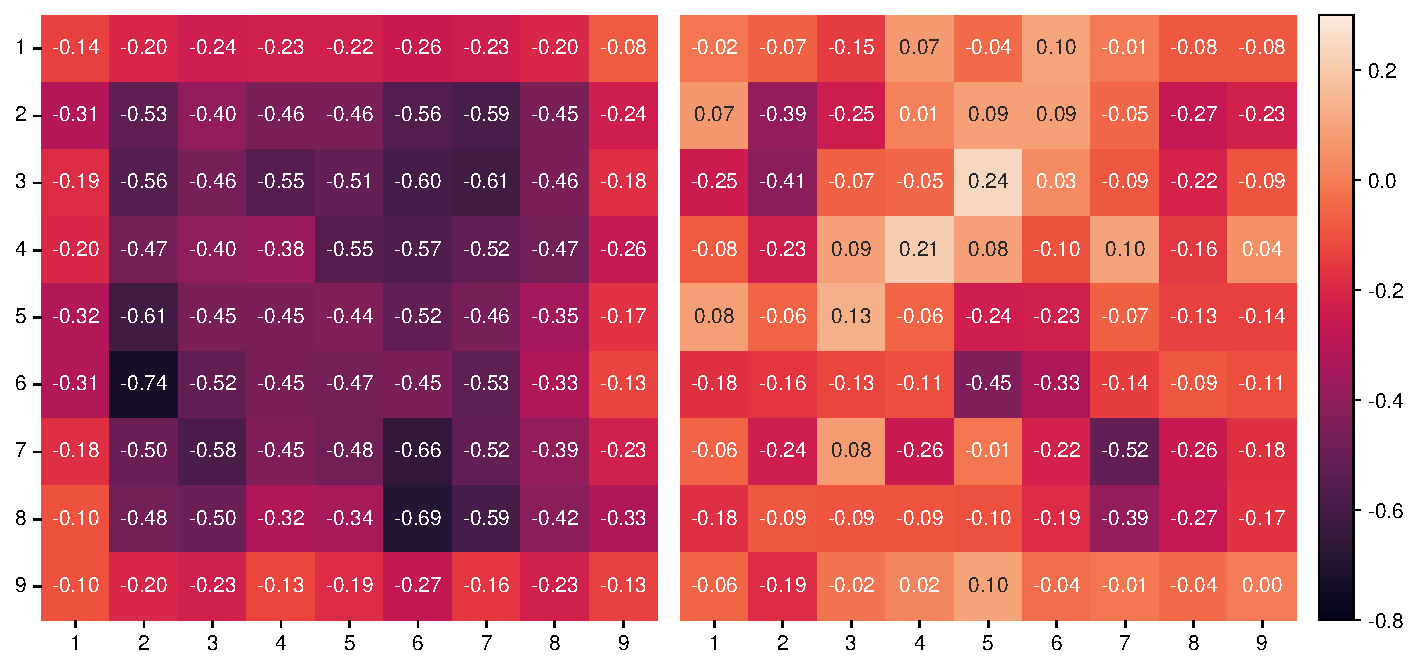
\includegraphics[width=\linewidth]{res/pictures/plots/21-action-ordering.pdf}
    \end{minipage}
    \begin{minipage}{.11\textwidth}
        \hfill
    \end{minipage}
    \captionof{figure}{Heatmap des Flicken 21}
    \label{fig:action-ordering-patch-21}
\end{figure}

\begin{figure}[!ht]
    \centering
    \begin{minipage}{.78\textwidth}
        \centering
        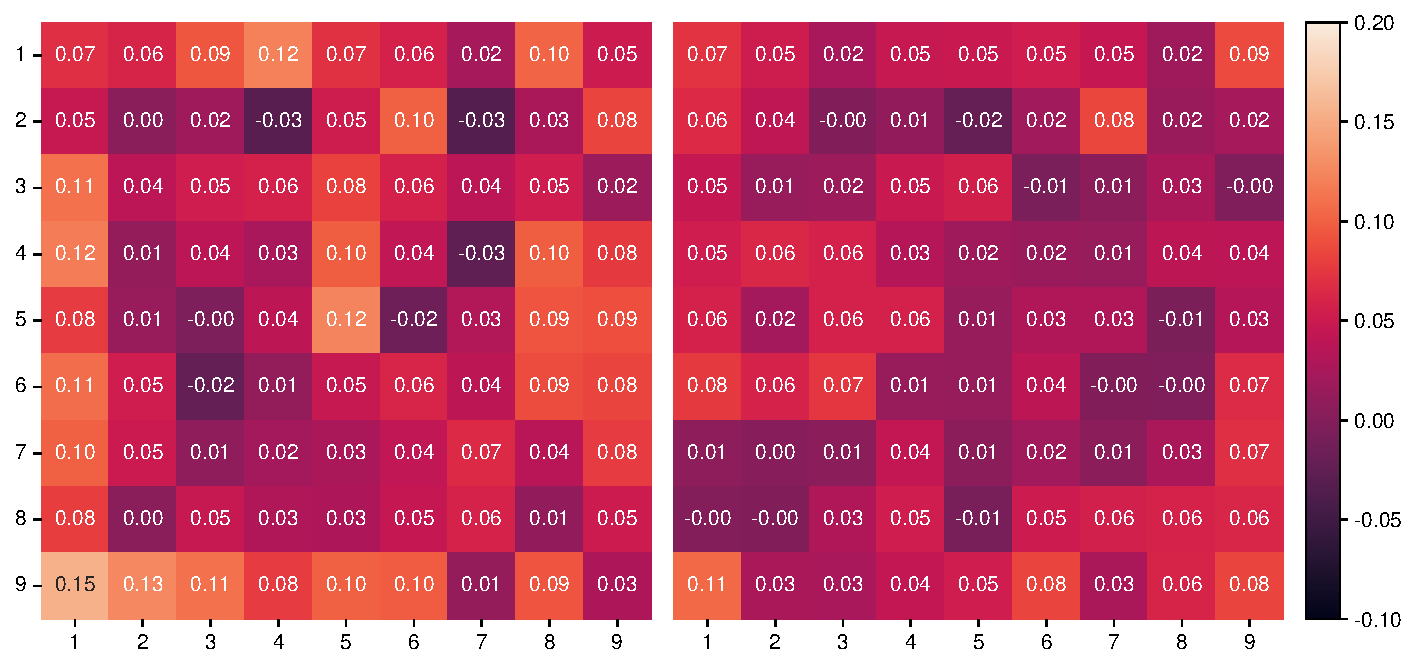
\includegraphics[width=\linewidth]{res/pictures/plots/special-action-ordering.pdf}
    \end{minipage}
    \captionof{figure}{Heatmap des Spezialflicken}
    \label{fig:action-ordering-special-patch}
\end{figure}

TODO:

\subsection{Transposition Table und Zobrist Hashing}

TODO:

\subsection{Aspiration Windows}

TODO:

\cite{2003.AspirationWindows}
\cite{2024.StockfishBackoff}

\pagebreak

\subsection{Suchselektivität}

Shannon führt in seinem Wert \emph{\enquote{Programming a Computer for Playing Chess}} eine Klassifizierung der Suchmethoden in einem Spielbaum ein, die zwei Haupttypen umfasst: \textbf{Typ-A} ist eine vollständige Brute-Force-Suche durch den gesamten Baum bis zu einer gewissen Tiefe \cite[S. 8]{1950.ChessShannon}. Bei der \textbf{Typ-B} werden die Äste des Spielbaums so selektiv ausgewählt, dass interessante Teilbäume tiefer durchsucht werden und uninteressante Teilbäume nur reduziert oder gar nicht durchsucht werden.

Im Bereich der Sucherweiterungen werden in Schach normalerweise Aktionen wie das Schlagen von Schachfiguren oder Schachsetzten berücksichtigt \cite[S. 14]{1950.ChessShannon}\cite{2023.StockfishTerminology}\cite{2003.SearchExtensions}. Während solche Aktionen in Patchwork nicht existieren, gibt es zwei Ereignisse, die für einen Spieler besonders interessant sind: Das Erhalten des $7\times 7$ Sonderplättchens sowie das Legen eines Spezialflicken. Bei beiden Aktionen wird die Suche deshalb um eine Tiefenebene erhöht (Anhang \ref{code:pvs-search-extension}). Im Fall der Null-Fenster-Suche werden keine Sucherweiterungen angewendet.

Für Patchwork sind Suchreduktionen im Bereich der Typ-B-Suche jedoch von größerer Bedeutung. Um bei Spielzuständen, die viele Aktionen erlauben und somit einen hohen Verzweigungsfaktor haben, den Suchaufwand möglichst minimal zu halten, sollte ein großer Teil der Aktionen nur reduziert durchsucht oder ganz weggelassen werden. Im \ac{PVS}-Spieler kommen hierzu zwei Konzepte zum Einsatz: \ac{LMR} und \ac{LMP}.

Bei einer Suche mit einigermaßen guter Zugreihenfolge tritt ein \hyperref[text:beta-cutoff]{\emph{Beta-Cutoff}} wenn überhaupt normalerweise am ersten \acs{PV}-Knoten auf \cite{2007.LMR}. Deswegen werden bei \ac{LMR} nur die ersten Aktionen mit der vollen Tiefe durchsucht und alle weiteren Aktionen werden insofern nichts interessantes passiert mit einer reduzierten Tiefe durchsucht. Als Nachteil muss aber bei einem zu guten Ergebnis über $\alpha$ der Teilbaum mit voller Tiefe erneut durchsucht werden \cite{2007.LMR}. Im \ac{PVS}-Spieler wird die Suche bei allen nicht \ac{PV}-Aktionen ab einer gewissen Tiefe auf ein Drittel der originalen Tiefe reduziert. Vorher wird die Suche immer um eine Ebene reduziert.

TODO:

\subsection{Lazy-SMP}

Der bisher beschriebene \ac{PVS}-Spieler läuft Single-Threaded ab. Da heutige Computer mehrere Kerne besitzen, sollten diese aber auch verwendet werden. Für Mimimax sowie davon abgeleitete Algorithmen existiert dazu eine einfache aber gleichzeitig effektive Parallelisierungsmöglichkeit.

Bei Lazy \ac{SMP}, werden $n$ parallele unabhängige Suchen gleichzeitig gestartet, welche sich nur die Transposition Table teilen. Dadurch, dass alle bereits durchsuchten Spielzustände in die Transposition Table eingefügt werden, wird sichergestellt, dass Spielzustände, welche zuvor von Threads erkundet wurden, nicht erneut durchsucht werden müssen.

TODO:

\section{Ansatz D: Monte Carlo Tree Search}
\label{section:erstellung-ansatz-c}

TODO:

\begin{itemize}
    \item Normaler MCTS
    \item UCT (Upper Confidence Bound for Trees)
    \item Parallel (Root und Leaf)
    \item Tree Reuse
    \item Evaluator (WinLoss, Score) -> In Eval genauer betrachten
\end{itemize}

\section{Ansatz E: AlphaZero}
\label{section:erstellung-ansatz-d}

TODO:

\begin{itemize}
    \item Änderungen Gegenüber MCTS / Generelle Funktionsweise
    \item Kodierung des Spielzustandes
    \item Netzwerk-Architektur
    \item Parallelization with Virtual Loss
    \item Training-Loop
\end{itemize}

\subsubsection*{Kodierung des Spielzustandes}

\begin{figure}[!ht]
    \centering
    \vspace*{-1.75cm}
    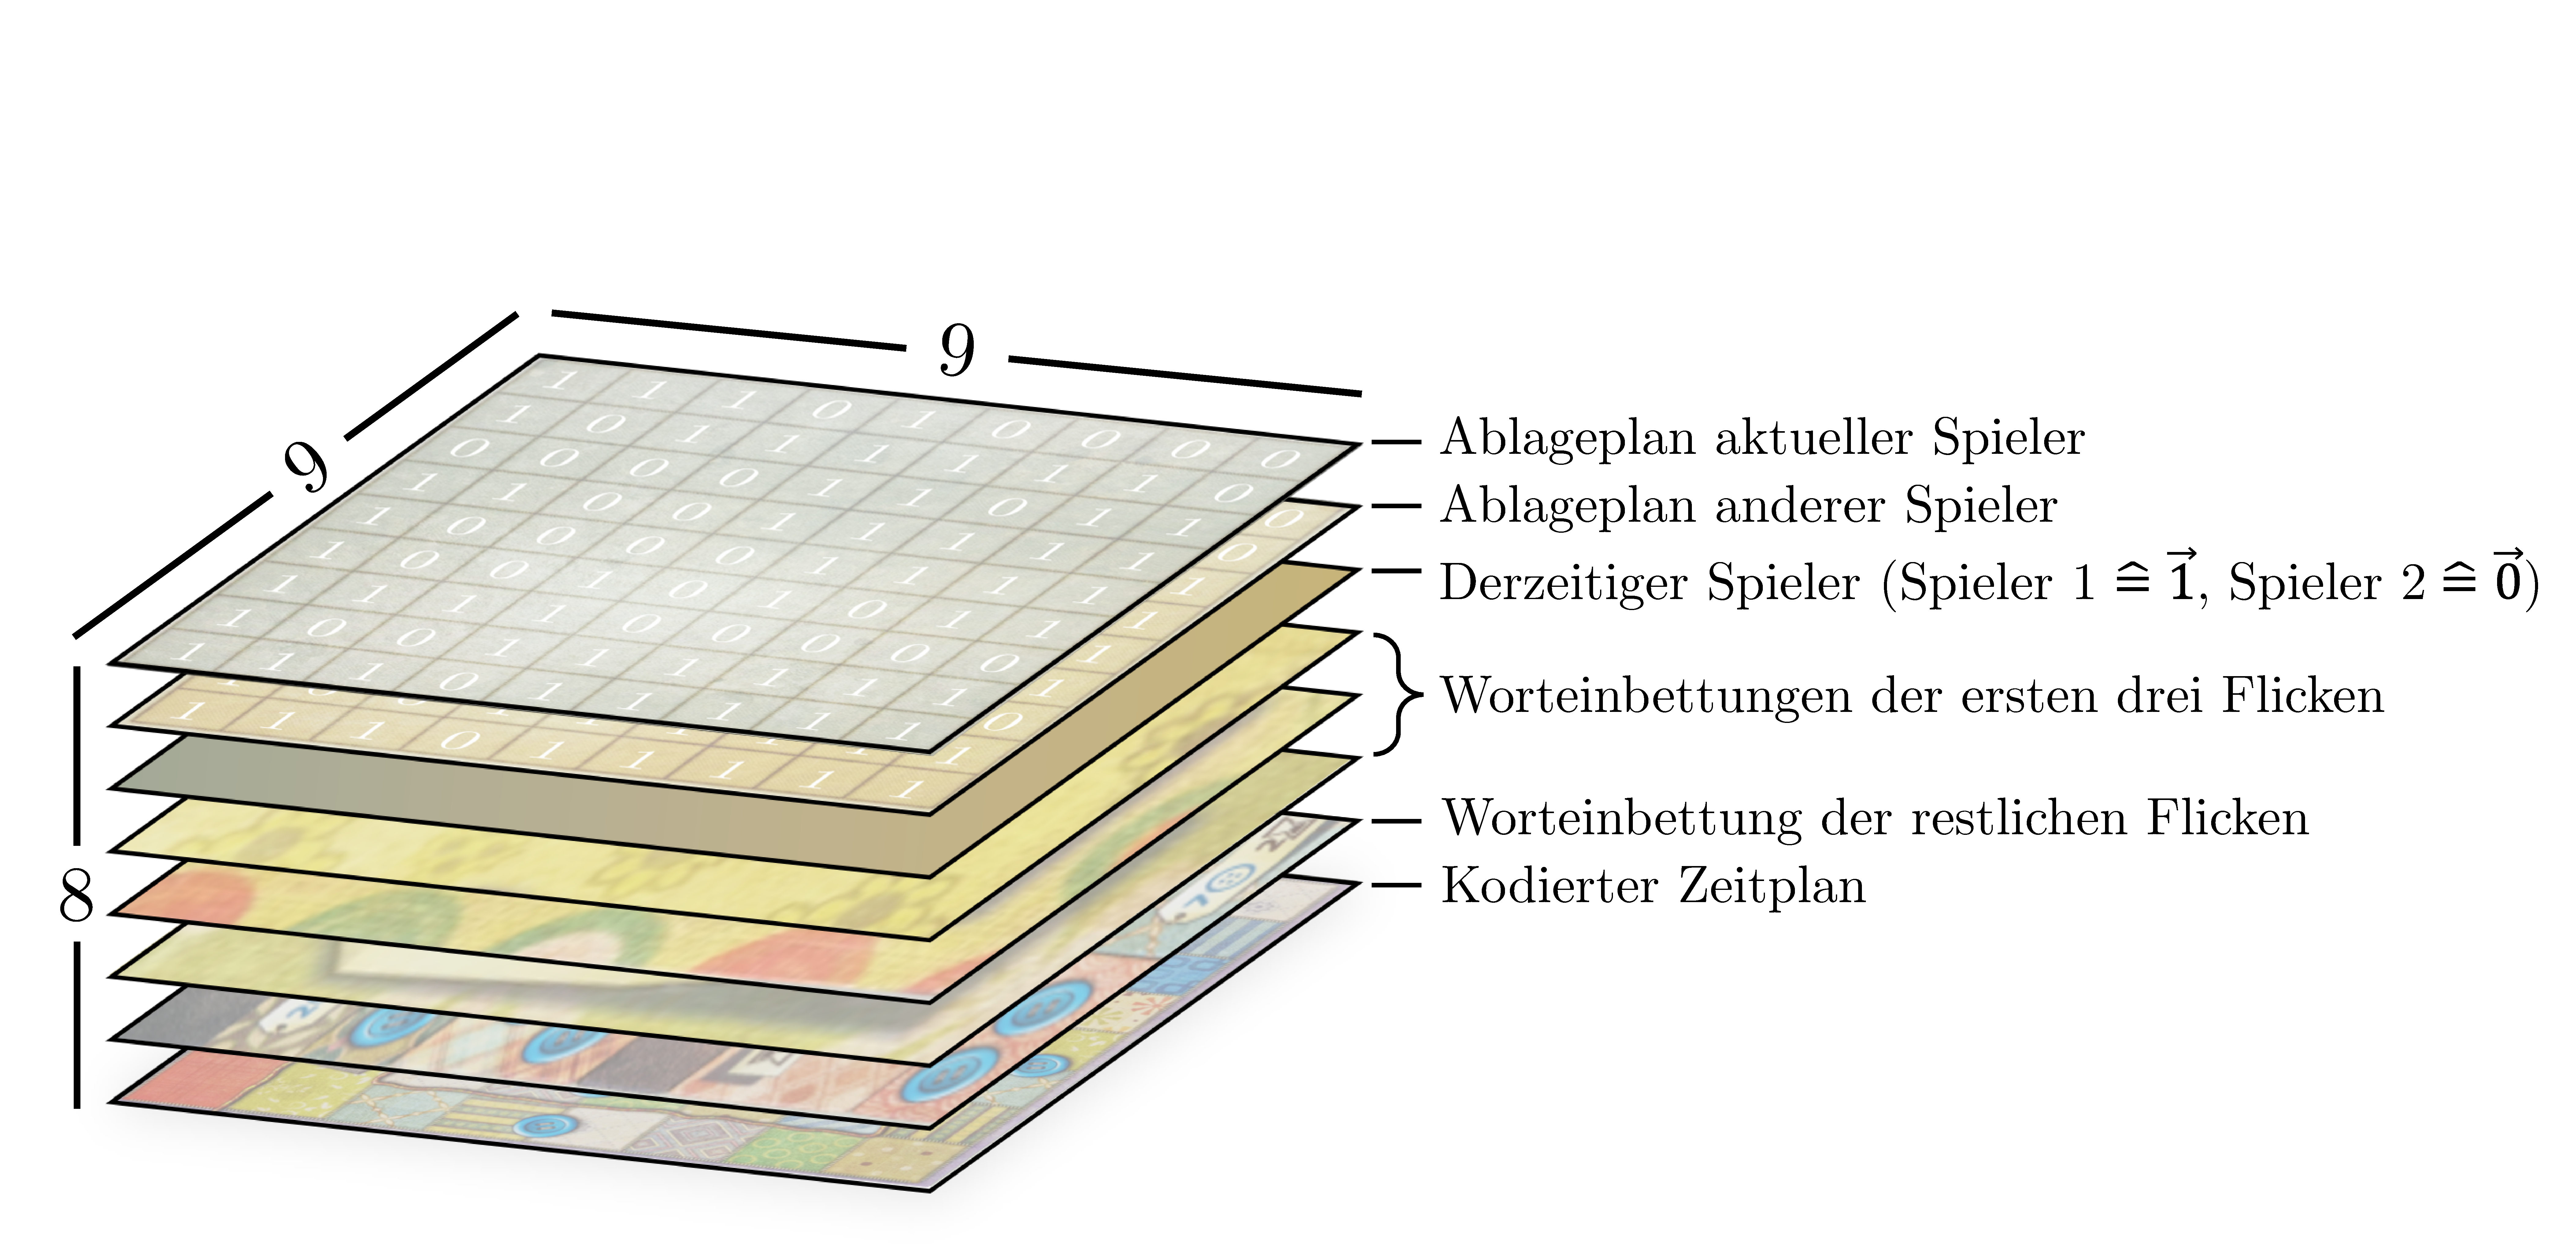
\includegraphics[width=\textwidth]{res/pictures/patch-zero-state.pdf}
    \caption{Zustandskodierung von PatchZero}
    \label{fig:patch-zero-state}
\end{figure}

TODO: LSTM Bild

\pagebreak

\subsubsection*{Netzwerk-Architektur}

\cite{2018.Lc0AlphaZero}
\cite{2019.SqueezeandExcitation}
\cite{2020.Lc0NetworkTopology}

\begin{figure}[!ht]
    \centering
    \includegraphics[width=\textwidth]{res/pictures/patch-zero-architecture.pdf}
    \caption{Architektur von PatchZero}
    \label{fig:patch-zero-architecture}
\end{figure}

TODO:

\begin{wrapfigure}{r}{0.25\textwidth}
    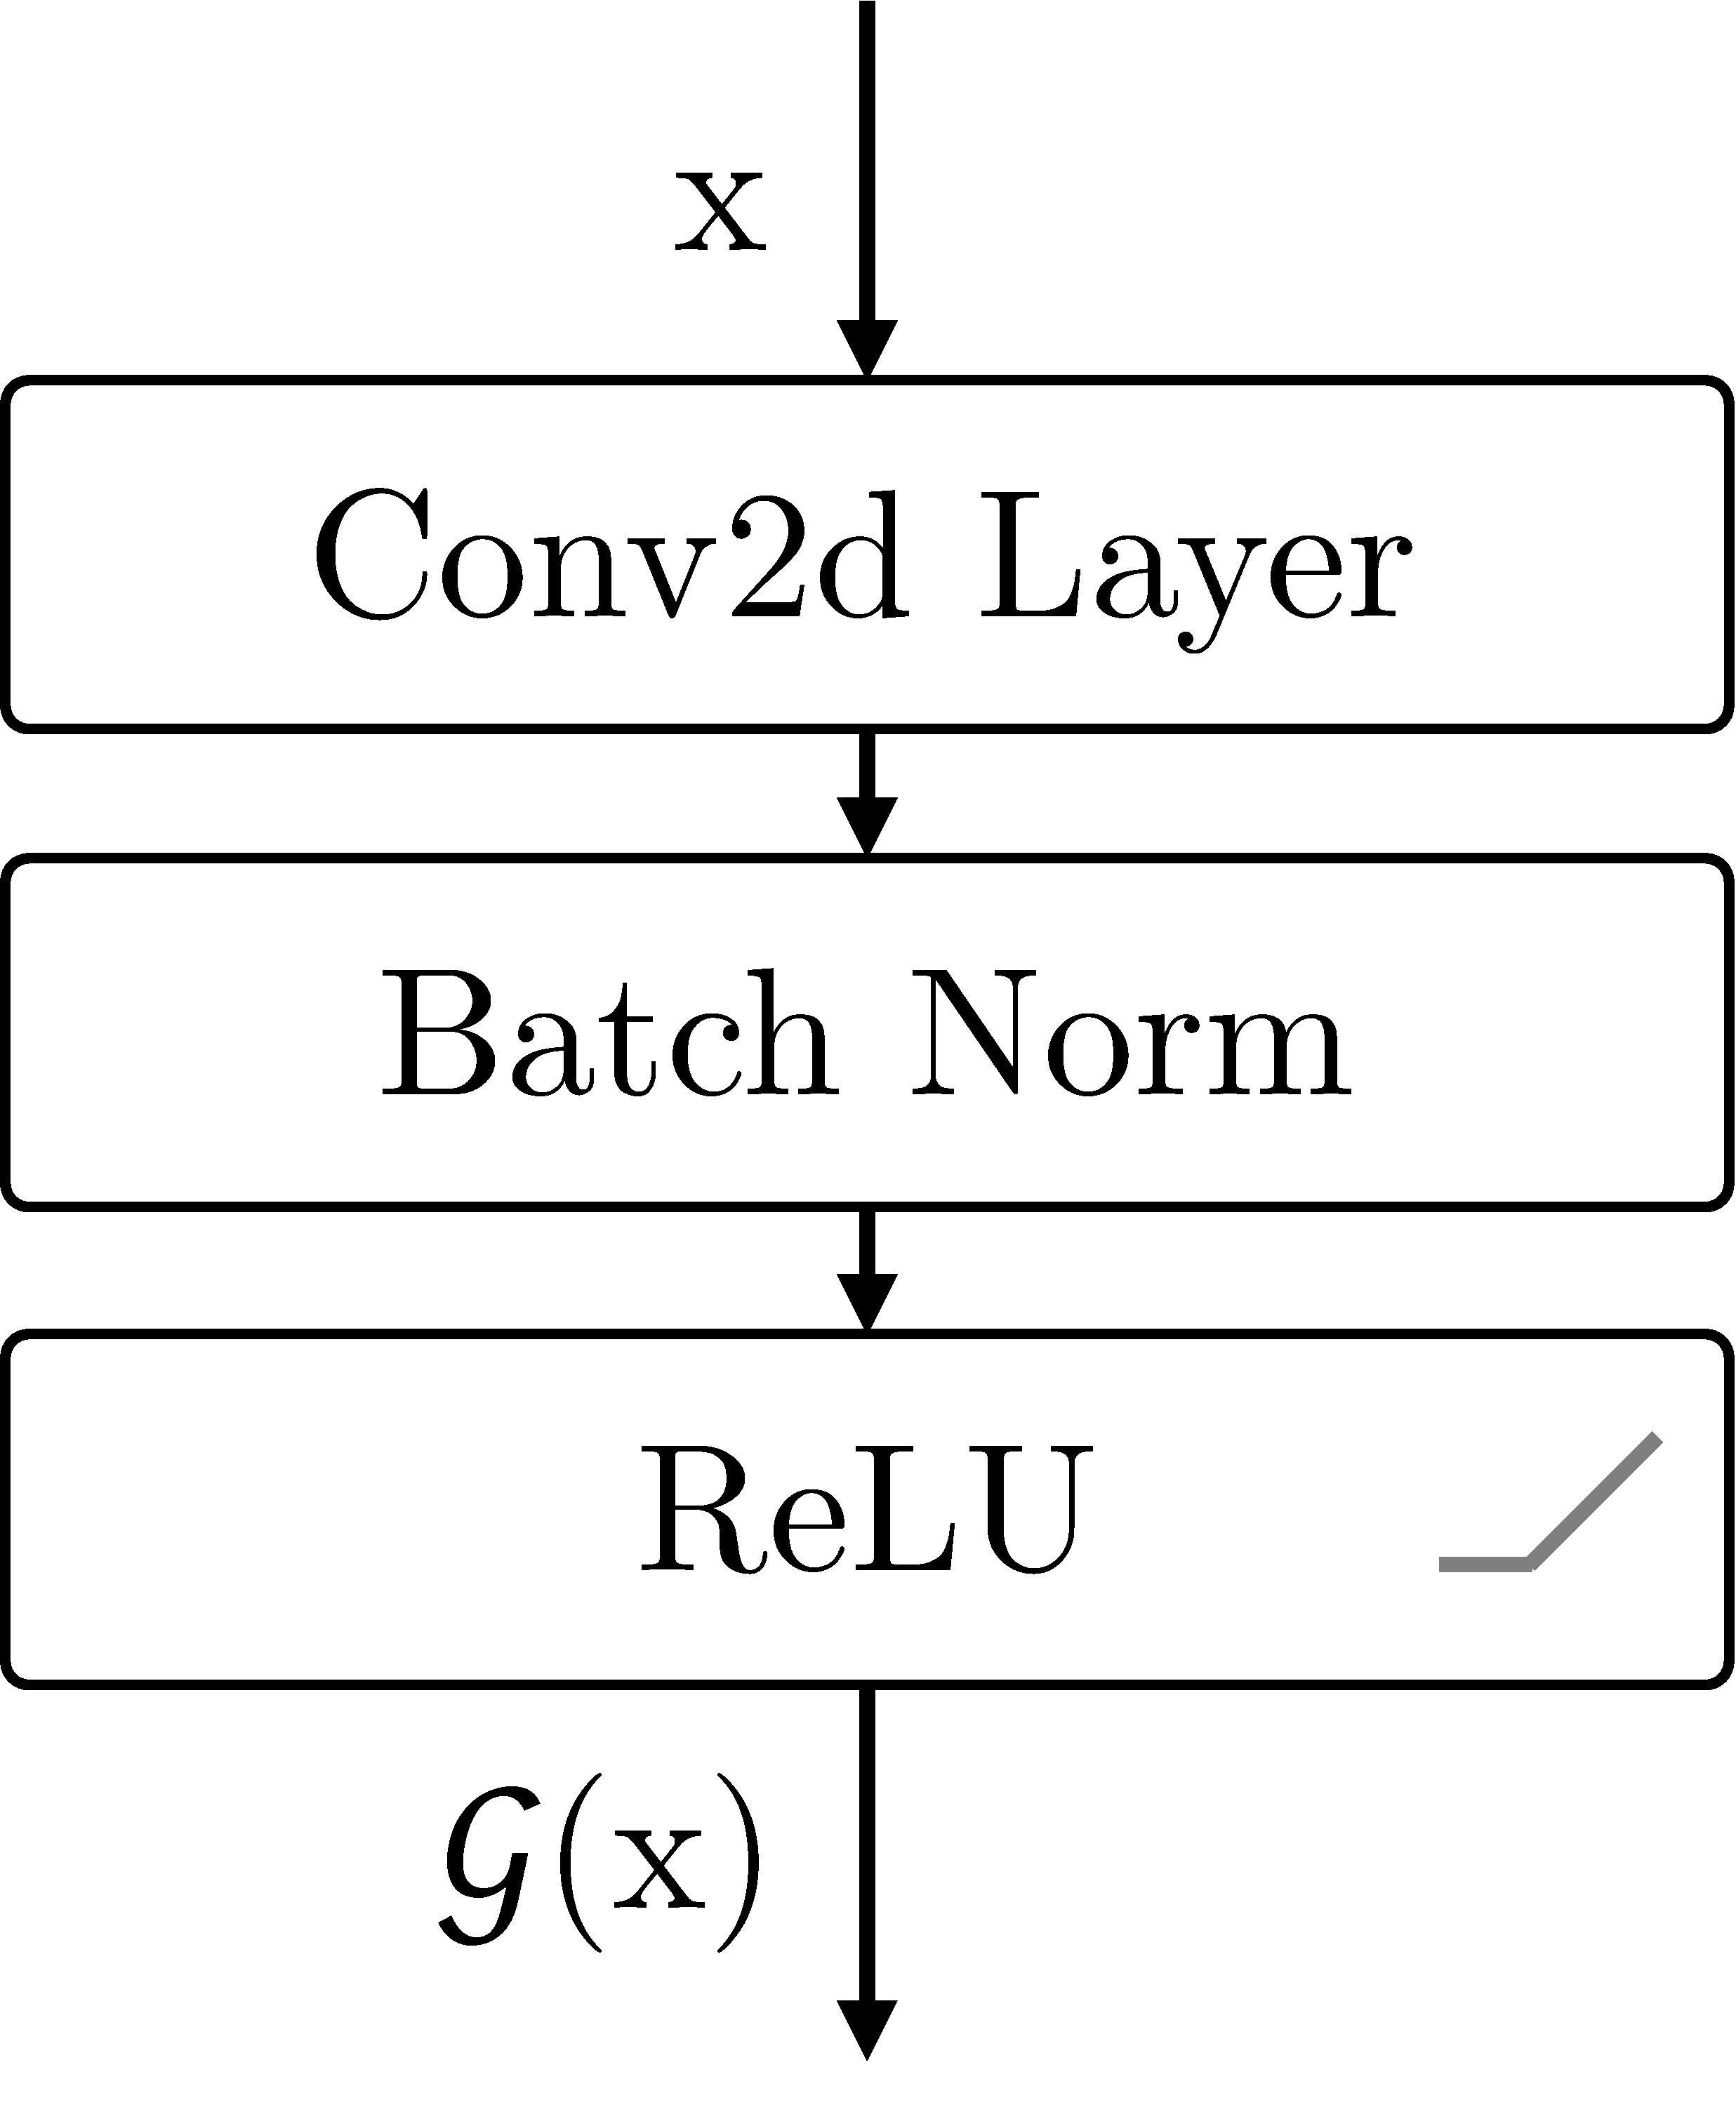
\includegraphics[width=0.2\textwidth]{res/pictures/conv-block.pdf}
    % \vspace{-10pt}
    % Das folgende ist ein Trick, um "Abbilgung x.y" in eine
    % eigene Zeile zu packen. Der Text zwischen [ und ] steht
    % im Abbildungsverzeichnis. Der Text darunter wird
    % tatsächlich angezeigt.
    \centering
    \caption[Convolutional Block]{\unskip}
    Convolutional Block
    \label{fig:conv-block}
\end{wrapfigure}

TODO:

\begin{wrapfigure}{l}{0.3\textwidth}
    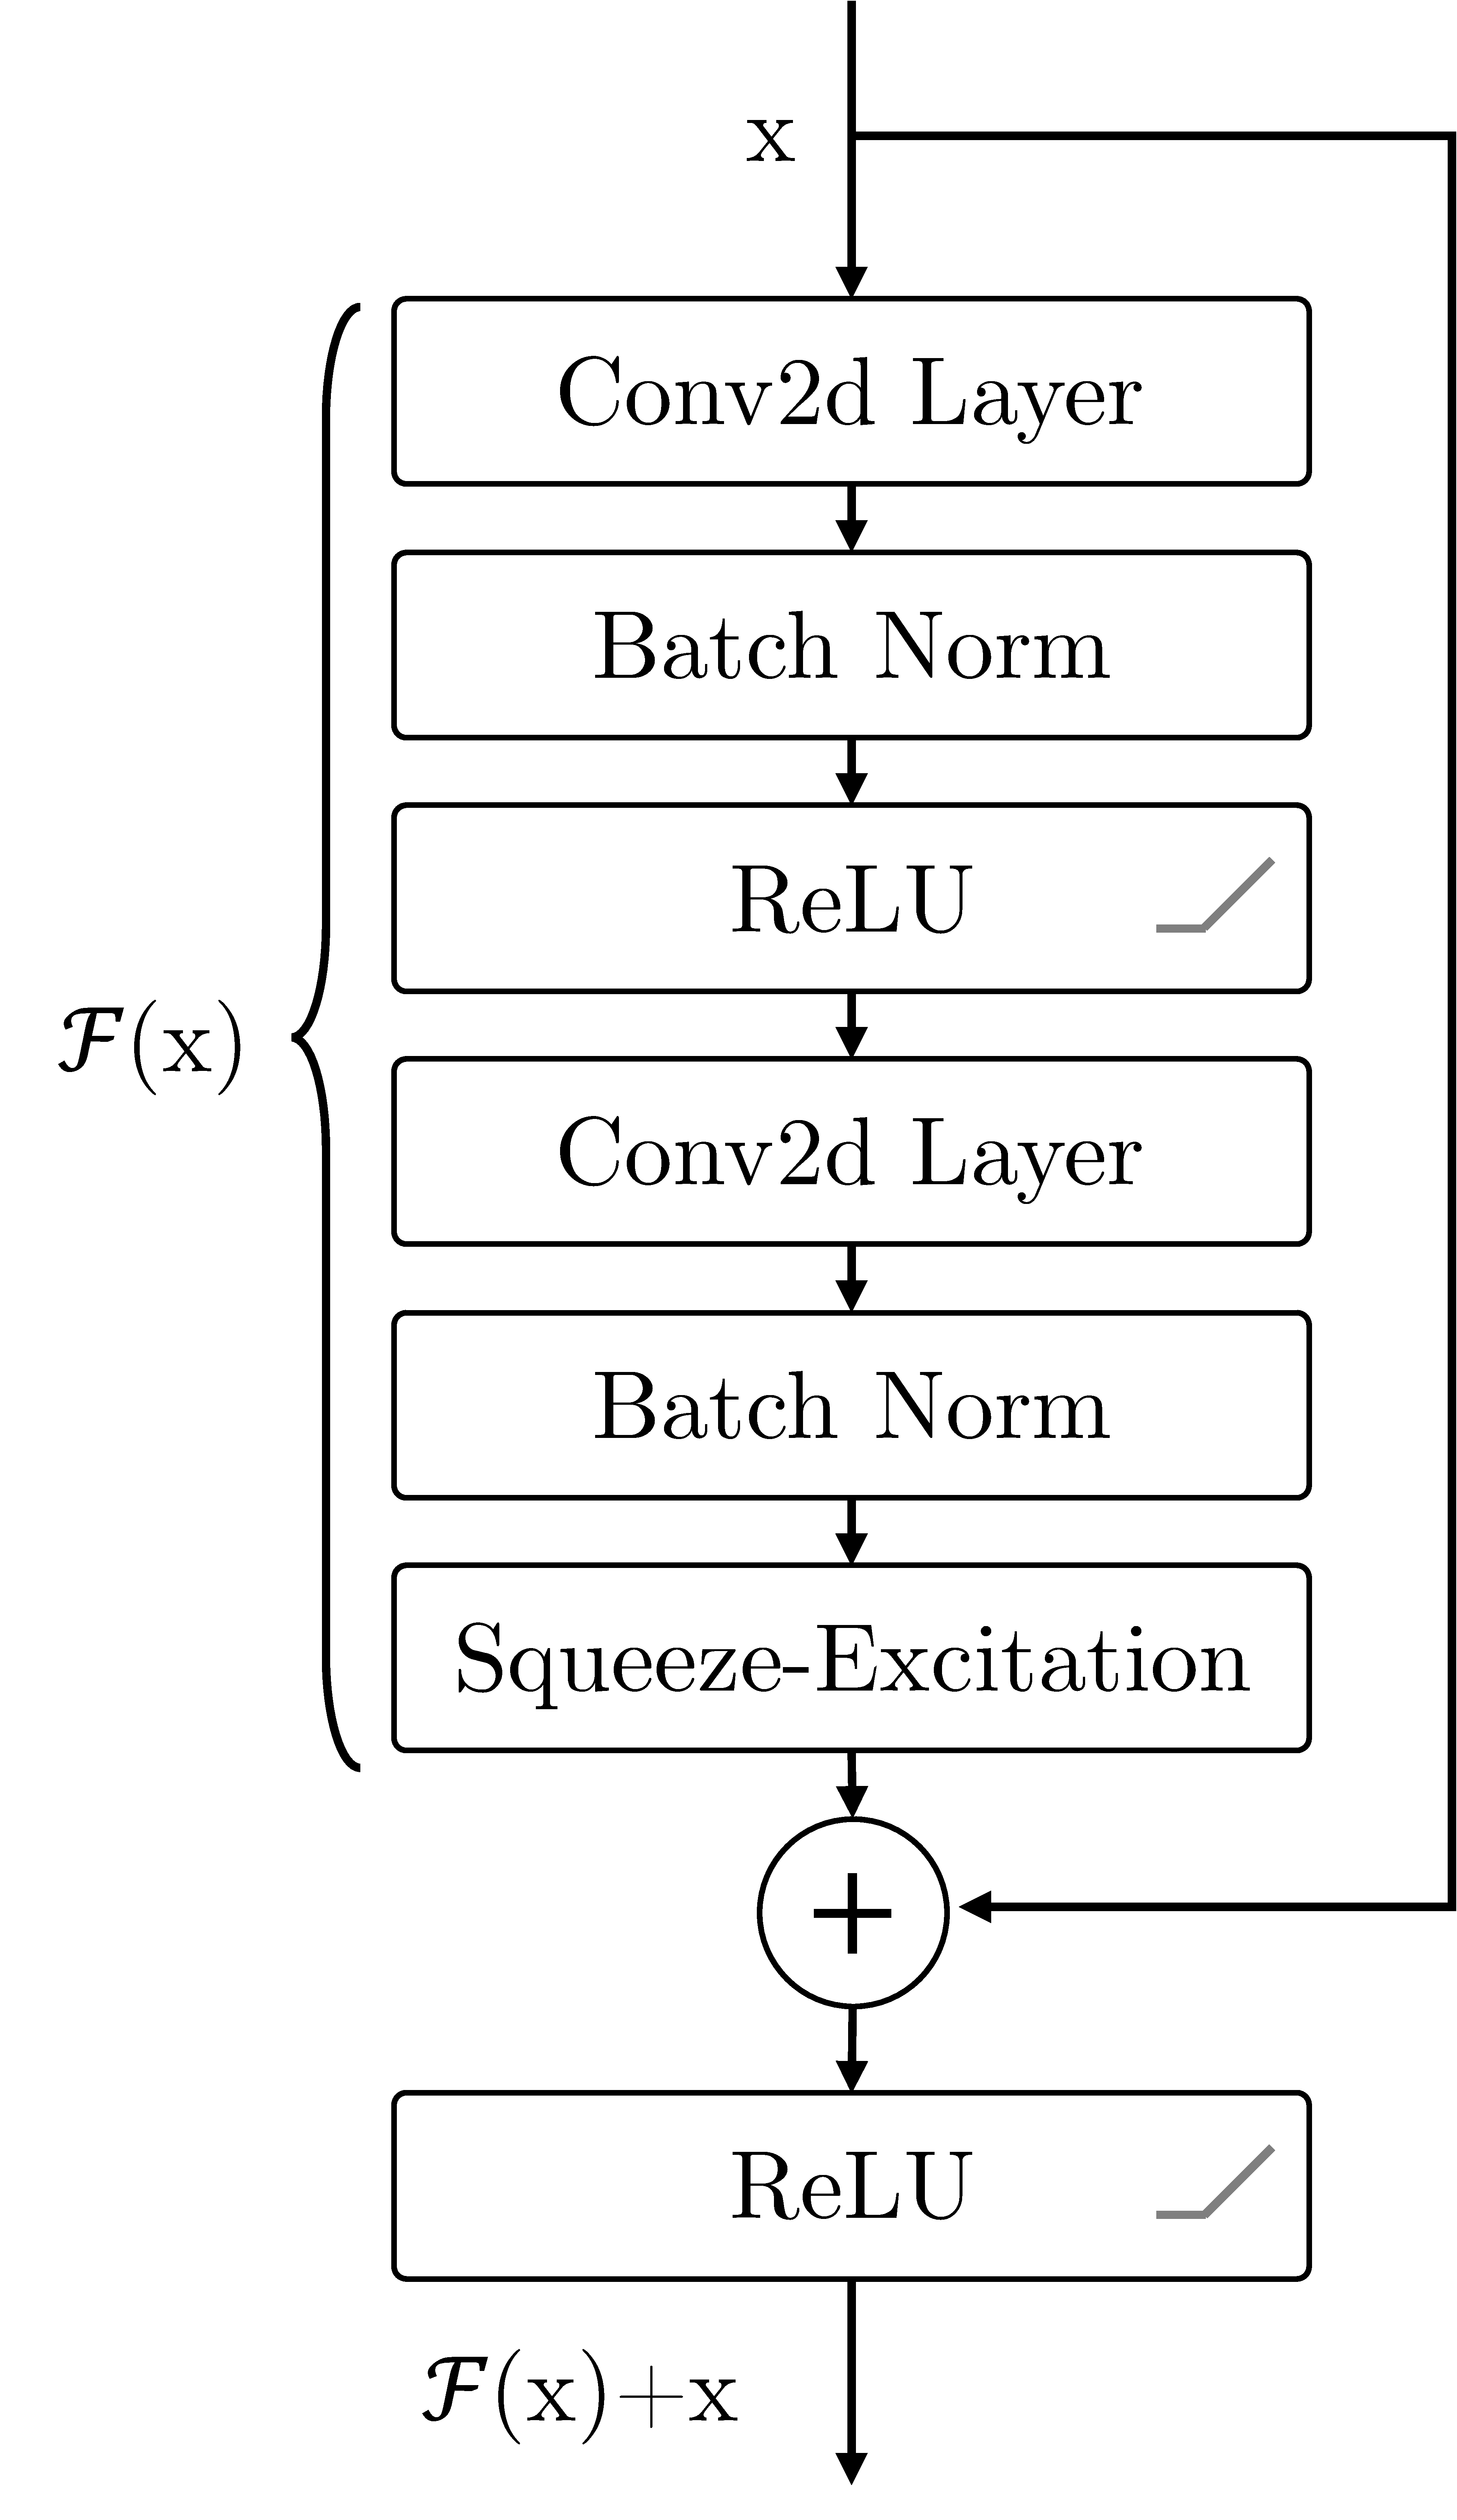
\includegraphics[width=0.25\textwidth]{res/pictures/res-block.pdf}
    % \vspace{-10pt}
    % Das folgende ist ein Trick, um "Abbilgung x.y" in eine
    % eigene Zeile zu packen. Der Text zwischen [ und ] steht
    % im Abbildungsverzeichnis. Der Text darunter wird
    % tatsächlich angezeigt.
    \centering
    \caption[Residual Block]{\unskip}
    Residual Block
    \label{fig:resblock}
\end{wrapfigure}

TODO:

\begin{wrapfigure}{r}{0.35\textwidth}
    \centering
    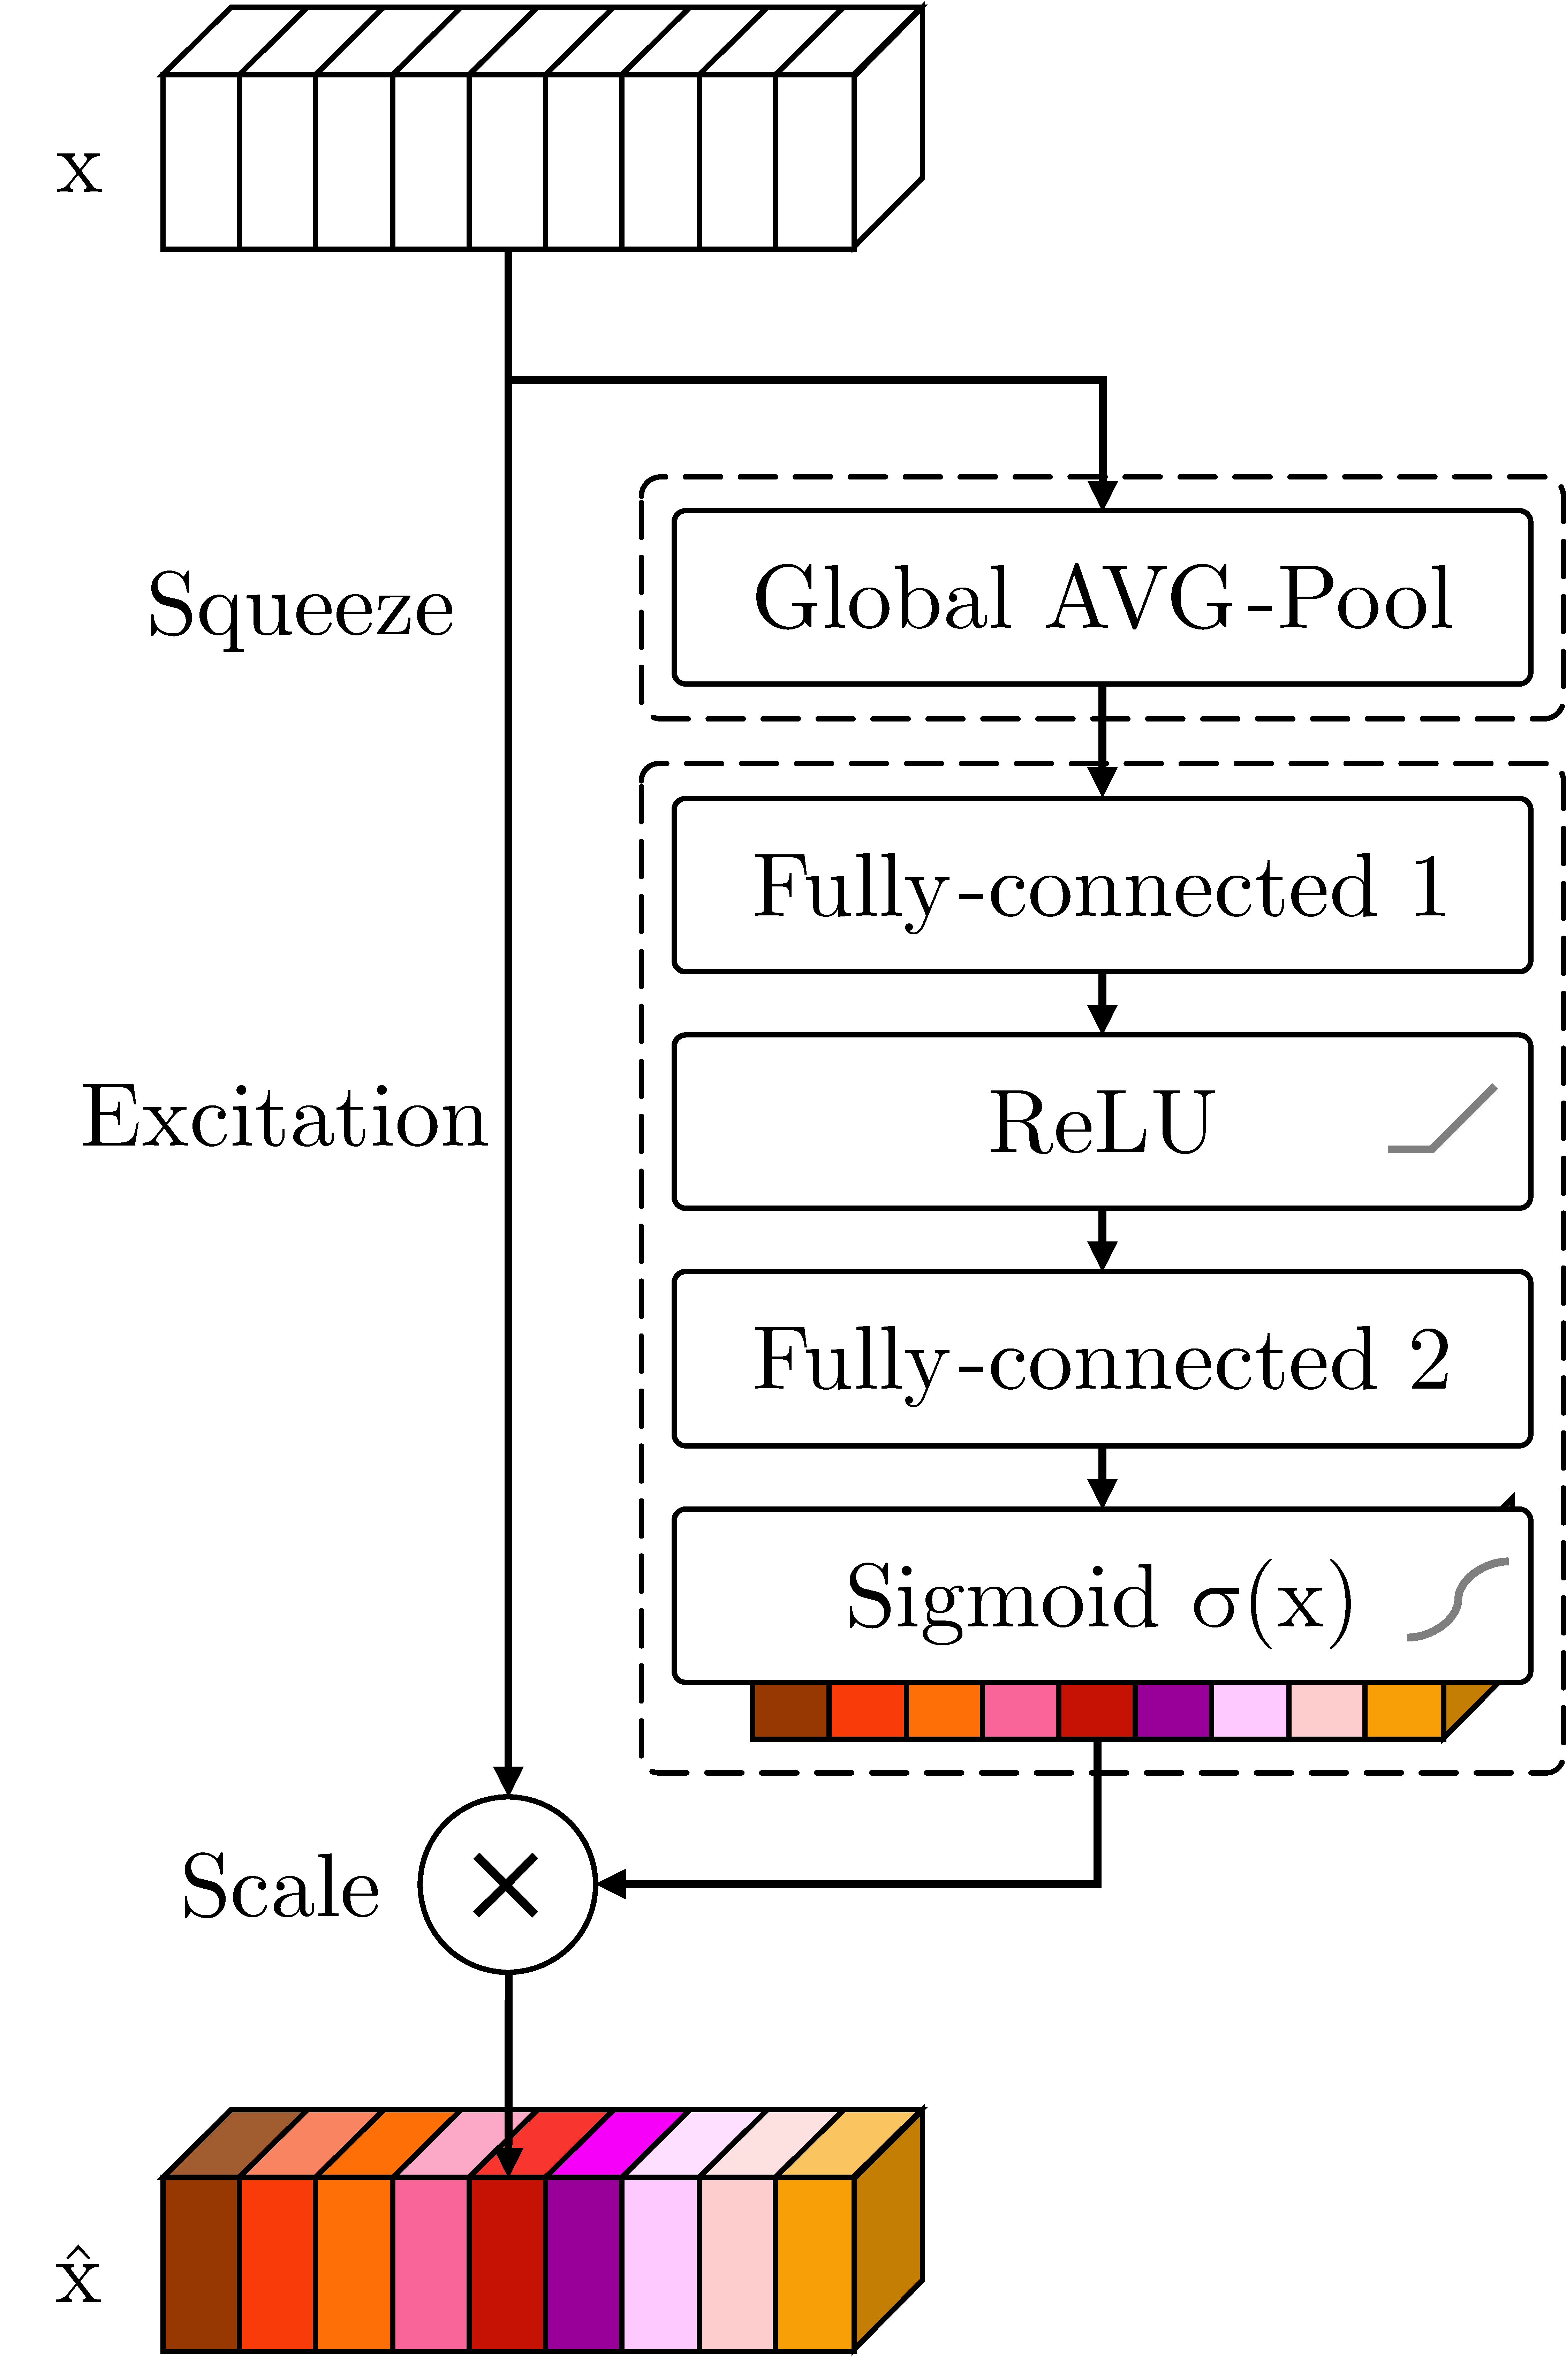
\includegraphics[width=0.3\textwidth]{res/pictures/squeeze-and-excitation-block.pdf}
    % \vspace{-10pt}
    % Das folgende ist ein Trick, um "Abbilgung x.y" in eine
    % eigene Zeile zu packen. Der Text zwischen [ und ] steht
    % im Abbildungsverzeichnis. Der Text darunter wird
    % tatsächlich angezeigt.
    \caption[Squeeze \& Excitation Block]{\unskip}
    Squeeze \& Excitation Block
    \label{fig:squeeze-and-excitation-block}
\end{wrapfigure}

TODO:

\pagebreak

\begin{figure}[!ht]
    \centering
    \includegraphics[width=0.7\textwidth]{res/pictures/value-and-policy-head.pdf}
    \\
    \begin{minipage}{.49\textwidth}
        \centering
        \captionof{figure}[Value Head von PatchZero]{\unskip}
        Value Head von PatchZero
        \label{fig:value-head}
    \end{minipage}
    \hfill
    \begin{minipage}{.49\textwidth}
        \centering
        \captionof{figure}[Policy Head von PatchZero]{\unskip}
        Policy Head von PatchZero
        \label{fig:policy-head}
    \end{minipage}
\end{figure}

TODO:
\chapter{Umsetzung der interaktiven Benutzeroberfläche}
\label{chapter:umsetzung-der-interaktiven-benutzeroberfläche}

{\color{white}
\begin{myverbbox}{\patchworkCLI}
The board game Patchwork implemented in Rust with different AI players. Type "help" for more information.
> console
Player 1: Human(name: Anonymer Modelleisenbahnliebhaber)
Player 2: Greedy
────────────────────────────────────────────────── TURN 1 ───────────────────────────────────────────────────
Current player is 1
...
────────────────────────────────────────────────── TURN 13 ──────────────────────────────────────────────────
Current player is 1
Player (button balance: 10): │ Player (button balance: 1):
  ▓▓▓█████▓⬜  │   ▓▓▓▓▓▓▓▓▓
  ███████▓▓⬜  │   ▓▓▓▓▓▓███
  █▓▓██▓▓▓▓⬜  │   ▓▓▓▓████▓
  ▓▓▓▓█▓▓▓▓⬜  │   ▓▓██████▓
  ▓▓▓▓▓▓▓▓▓⬜  │   ▓▓███████
  ▓▓▓▓▓▓▓▓▓⬜  │   ▓▓██████▓
  ▓▓▓▓▓▓▓▓▓⬜  │   ▓▓▓█▓▓█▓▓
  ▓▓▓▓▓▓▓▓▓⬜  │   ▓▓▓▓▓▓▓▓▓
  ▓▓▓▓▓▓▓▓▓⬜  │   ▓▓▓▓▓▓▓▓▓
      Button income: 0       │      Button income: 3
Time board:
┌─┬─┬─┬─┬─┬─┬─┬─┬─┬─┬─┬─┬─┬─┬─┬─┬─┬─┬─┬─┬─┬─┬─┬─┬─┬─┬─┬─┬─┬─┬─┬─┬─┬─┬─┬─┬─┬─┬─┬─┬─┬─┬─┬─┬─┬─┬─┬─┬─┬─┬─┬─┬─┬─┐
│ │ │ │ │ │B│ │ │ │ │ │B│ │ │ │1│2│B│ │ │ │ │ │B│ │ │P│ │ │B│ │ │P│ │ │B│ │ │P│ │ │B│ │ │P│ │ │B│ │ │P│ │ │B│
└─┴─┴─┴─┴─┴─┴─┴─┴─┴─┴─┴─┴─┴─┴─┴─┴─┴─┴─┴─┴─┴─┴─┴─┴─┴─┴─┴─┴─┴─┴─┴─┴─┴─┴─┴─┴─┴─┴─┴─┴─┴─┴─┴─┴─┴─┴─┴─┴─┴─┴─┴─┴─┴─┘
Next 6 patches (can only take first 3):
⬜█⬜⬜        ⬜⬜⬜⬜        ⬜⬜⬜⬜        █⬜⬜⬜        ██
⬜█⬜⬜        ⬜⬜⬜⬜        ⬜⬜⬜⬜        █⬜⬜⬜        ██
⬜█⬜⬜        █⬜⬜⬜        ██⬜⬜        ██⬜⬜        ⬜█⬜⬜         ⬜█
███⬜        ███⬜        ██⬜⬜        █⬜⬜⬜        ⬜█⬜⬜         ██
Id: 12            Id: 19            Id: 9             Id: 10            Id: 13             Id: 21
Income: 2         Income: 1         Income: 2         Income: 1         Income: 3          Income: 0
Button cost: 7    Button cost: 4    Button cost: 6    Button cost: 2    Button cost: 10    Button cost: 1
Time cost: 2      Time cost: 2      Time cost: 5      Time cost: 3      Time cost: 5       Time cost: 3
'Anonymer Modelleisenbahnliebhaber' can choose one of the actions: 'take 1', 'take 2', 'take 3', 'walk'.
> Please enter the action: take 2
You chose to place the following patch:
   █⬜⬜   Id: 19       Button cost: 4
   ███   Income: 1    Time cost: 2
> Please enter the  rotation (0, 90, 180, 270) and orientation (if flipped: y/n) of the patch: 0,n
> Please enter the row and column of the patch (row, column): 5,5
Player 'HumanPlayer(name: Anonymer Modelleisenbahnliebhaber)' chose action:
Action 402 - Patch(12) placement (index 0) at (4, 4) with (R 0°, O normal) (P12I0═4‖4↻0↔0P1) after 15.95s
\end{myverbbox}
}

\definecolor{maximizeWindowColor}{HTML}{f5df09}
\definecolor{minimizeWindowColor}{HTML}{56bd73}
\definecolor{closeWindowColor}{HTML}{ea4f44}

\begin{figure}[!ht]
    \centering
    \resizebox{\textwidth}{!}{\begin{tikzpicture}
            \node [text=white,inner sep=0pt,,outer sep=0pt,clip,rounded corners=0.15cm] (cli) at (0,0) {\sffamily \patchworkCLI};
            \node[circle,fill=closeWindowColor, minimum size = 0.15cm, above right = 0.3cm and -0.3cm of cli] (close) {};
            \node[circle,fill=maximizeWindowColor, minimum size = 0.15cm, left = 0.15cm of close] (maximize) {};
            \node[circle, fill=minimizeWindowColor, minimum size = 0.15cm, left = 0.15cm of maximize] {};
            \node[text=white] at ($ (cli.north) + (0,0.45) $) {\sffamily \textbf{Patchwork 1.0.0 (Release Build) | Fabian Wolf \& Nico Zeitz}} ;
            \begin{pgfonlayer}{back}
                \filldraw[fill=black,draw=black,rounded corners=0.15cm] ($ (cli.north west) + (-0.25,0.85) $) rectangle ($ (cli.south east) + (0.25,-0.25) $);
            \end{pgfonlayer}
            \begin{pgfonlayer}{shadow}
                \shade[outercolor,inner color=innercolor,outer color=outercolor] ($(cli.south west)+(-0.25,0.25)+(\shadowshift)+(\shadowradius/2,\shadowradius/2)$) circle (\shadowradius);
                \shade[outercolor,inner color=innercolor,outer color=outercolor] ($(cli.north west)+(-0.25,0.85)+(\shadowshift)+(\shadowradius/2,-\shadowradius/2)$) circle (\shadowradius);
                \shade[outercolor,inner color=innercolor,outer color=outercolor] ($(cli.south east)+(0.25,0.25)+(\shadowshift)+(-\shadowradius/2,\shadowradius/2)$) circle (\shadowradius);
                \shade[outercolor,inner color=innercolor,outer color=outercolor] ($(cli.north east)+(0.25,0.85)+(\shadowshift)+(-\shadowradius/2,-\shadowradius/2)$) circle (\shadowradius);
                \shade[top color=innercolor,bottom color=outercolor] ($(cli.south west)+(-0.25,0.25)+(\shadowshift)+(\shadowradius/2,-\shadowradius/2)$) rectangle ($(cli.south east)+(0.25,0.25)+(\shadowshift)+(-\shadowradius/2,\shadowradius/2)$);
                \shade[left color=innercolor,right color=outercolor] ($(cli.south east)+(0.25,0.25)+(\shadowshift)+(-\shadowradius/2,\shadowradius/2)$) rectangle ($(cli.north east)+(0.25,0.85)+(\shadowshift)+(\shadowradius/2,-\shadowradius/2)$);
                \shade[bottom color=innercolor,top color=outercolor] ($(cli.north west)+(-0.25,0.85)+(\shadowshift)+(\shadowradius/2,-\shadowradius/2)$) rectangle ($(cli.north east)+(0.25,0.85)+(\shadowshift)+(-\shadowradius/2,\shadowradius/2)$);
                \shade[outercolor,right color=innercolor,left color=outercolor] ($(cli.south west)+(-0.25,0.25)+(\shadowshift)+(-\shadowradius/2,\shadowradius/2)$) rectangle ($(cli.north west)+(-0.25,0.85)+(\shadowshift)+(\shadowradius/2,-\shadowradius/2)$);
                \filldraw ($(cli.south west)+(-0.25,0.25)+(\shadowshift)+(\shadowradius/2,\shadowradius/2)$) rectangle ($(cli.north east)+(0.25,0.85)+(\shadowshift)-(\shadowradius/2,\shadowradius/2)$);
            \end{pgfonlayer}
        \end{tikzpicture}}
    \caption[CLI Schnittstelle des Patchwork Spiels]{\acs{CLI} Schnittstelle des Patchwork Spiels}
    \label{fig:patchwork-console-ui}
\end{figure}

Bei der Gestaltung der interaktiven Benutzeroberfläche wurde ein großer Fokus auf ein selbsterklärendes und intuitives Design gelegt, was auf Grundlage des Wissens aus dem Kapitel \ref{chapter:interaktive-systeme} umgesetzt wurde. Zuvor wurde allerdings als erste, einfache Interaktionsmöglichkeit mit dem Computerspiel die Steuerung über ein \ac{CLI} ermöglicht. In der Abbildung \ref{fig:patchwork-console-ui} ist der Start eines neuen Patchwork-Spiels und ein weiter vorgeschrittener Zug innerhalb dieses Spiels zu sehen. Die Einstellung für das Spiel werden hier am Anfang durch Eingabe der gewünschten Computergegner mit entsprechenden Spezifikationen getroffen. Dann werden für jeden Zug angezeigt, wie die Ablagepläne der beiden Spieler aussehen, wie weit sie auf dem Zeitplan fortgeschritten sind, wobei die beiden Zahlen die Spieler repräsentieren, während B ein Knopfeinkommen und P eine Stelle mit Spezialflicken bezeichnet. Darauffolgend werden die ersten drei wählbaren Flicken und noch drei weitere mit allen dazugehörigen Informationen dargestellt, damit der Spieler sich überlegen kann welche Aktion getätigt werden soll. Die ausgewählte Aktion muss anschließend gegebenenfalls noch durch weitere Angaben spezifiziert werden, um den Spielzug abzuschließen. Diese Möglichkeit der Interaktion mit dem Computerspiel wurde als vorübergehende Lösung bis zur Fertigstellung der tatsächlichen Benutzeroberfläche konzeptioniert und umgesetzt.

\begin{figure}[!ht]
    \centering
    \resizebox{\textwidth}{!}{\begin{tikzpicture}
        \node [inner sep=0pt,,outer sep=0pt,clip,rounded corners=0.15cm] (image) at (0,0) {
            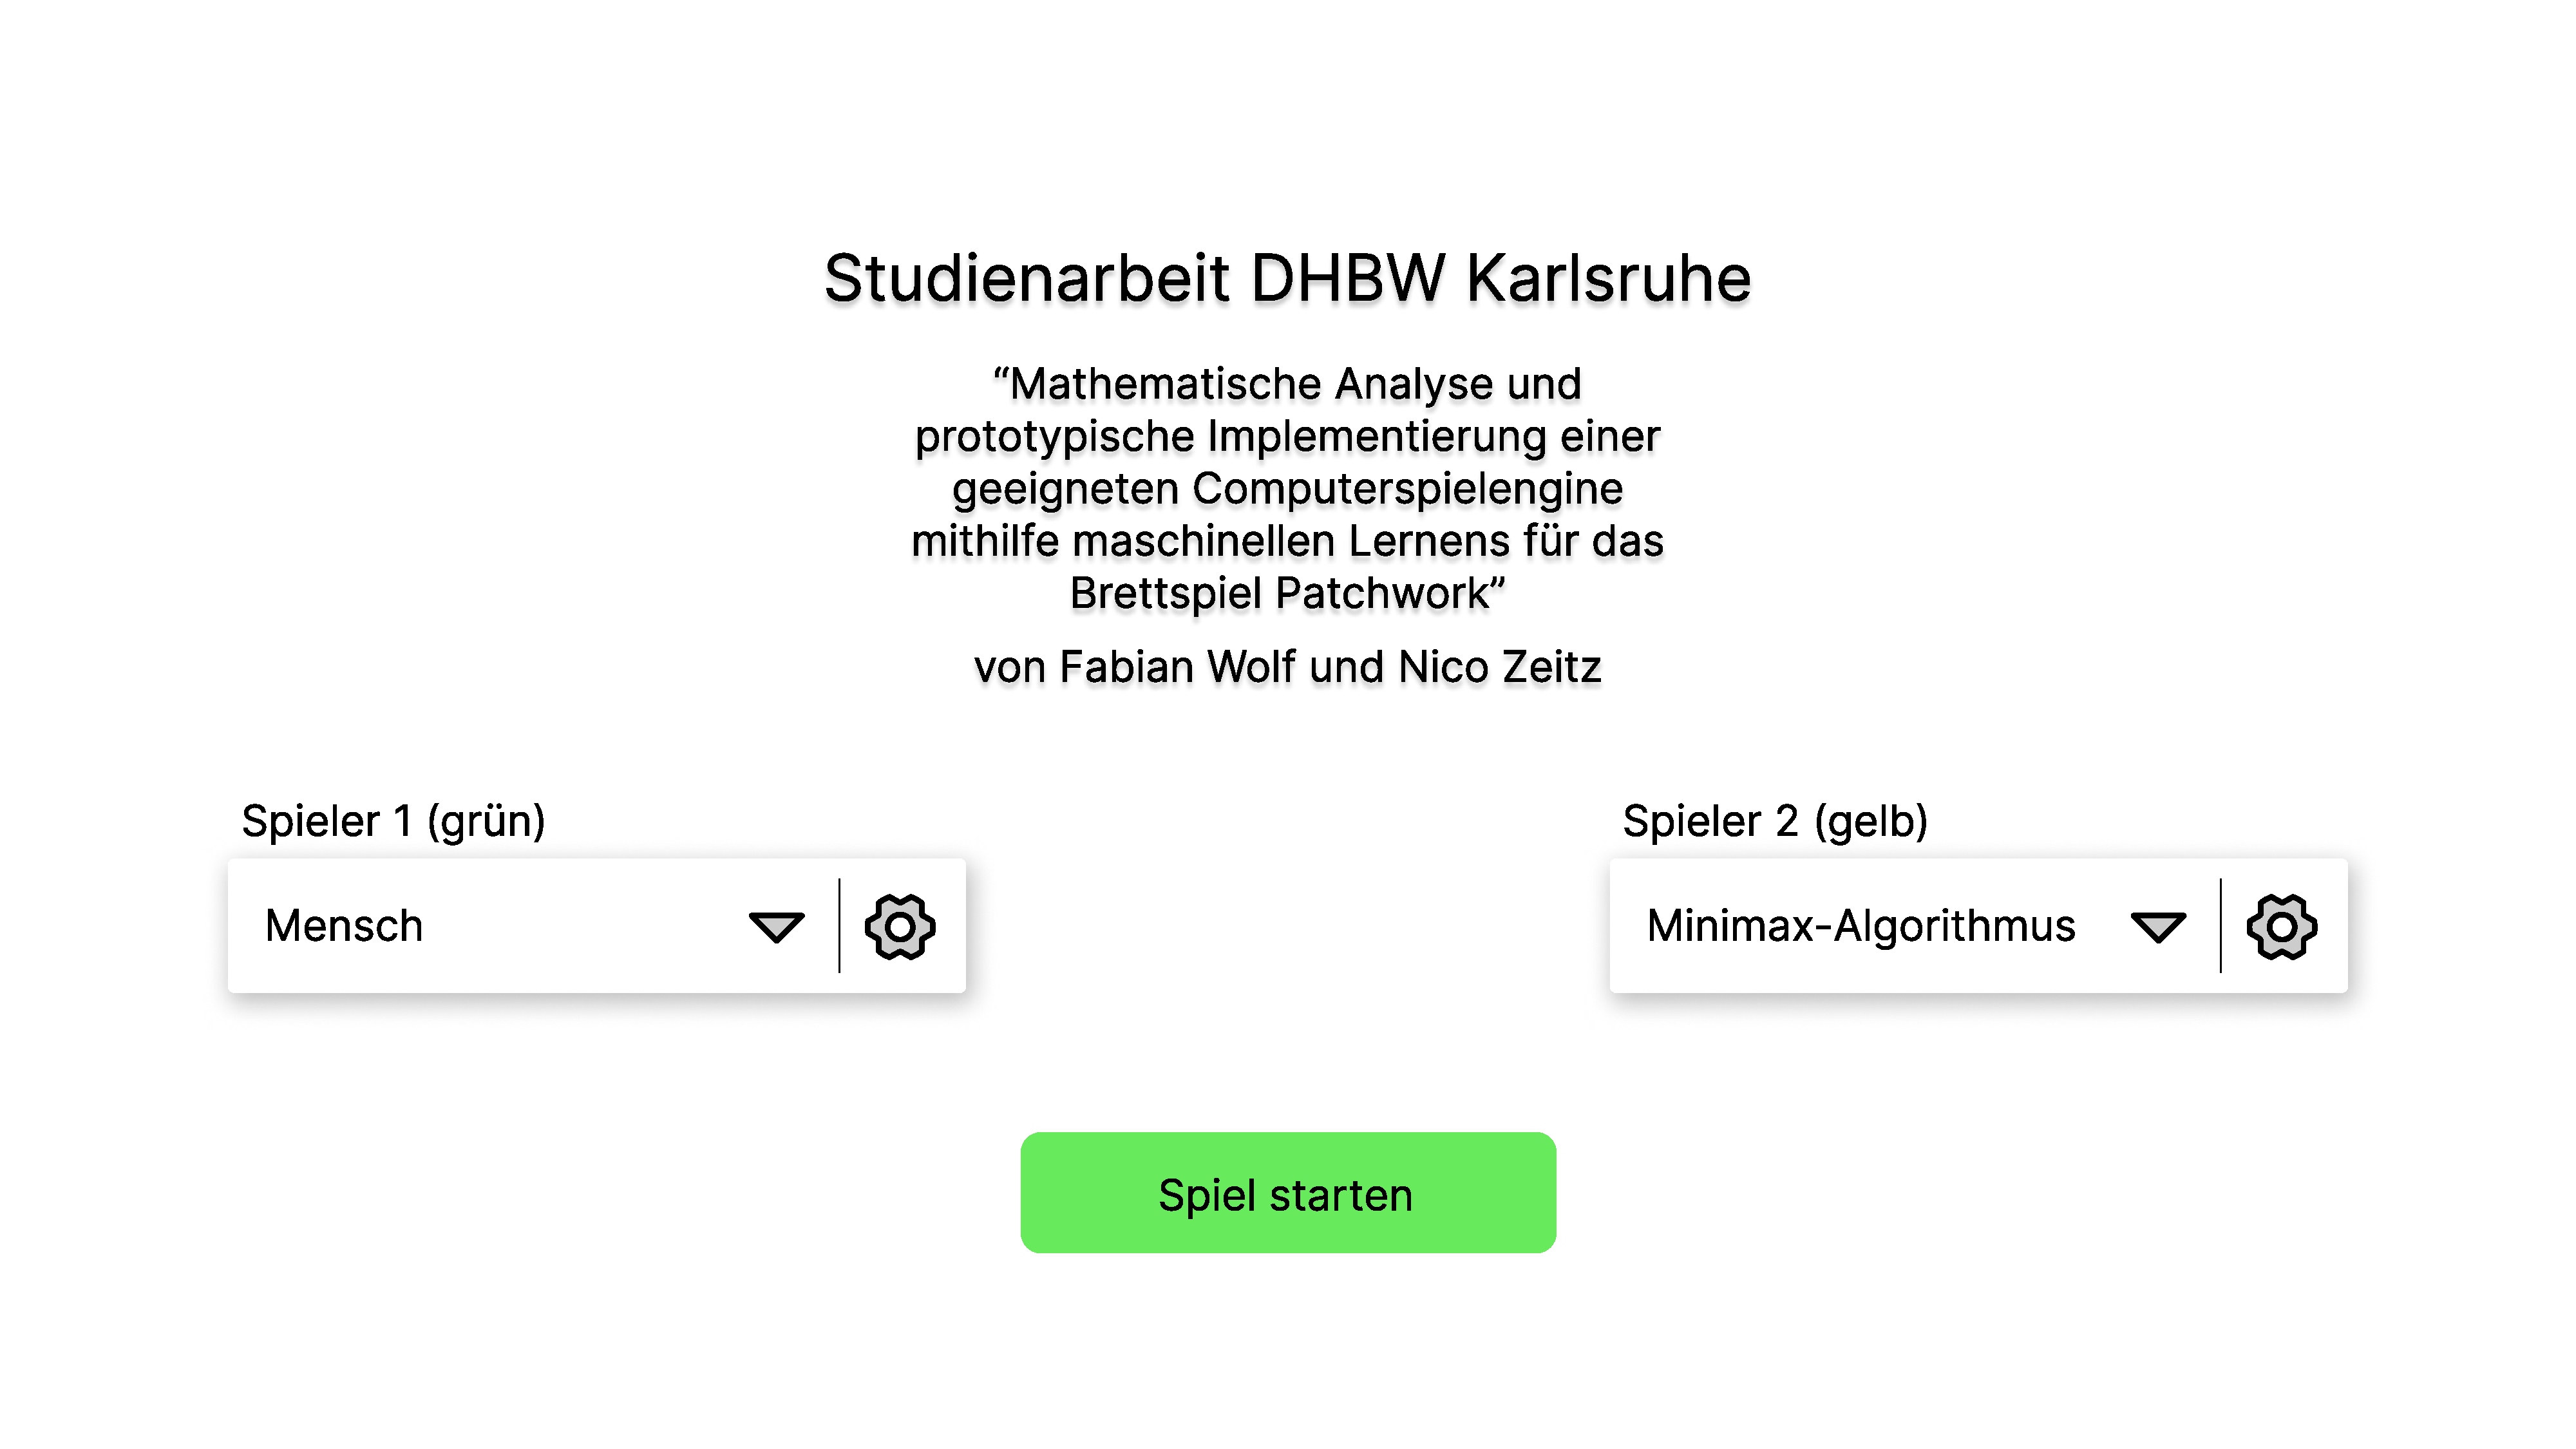
\includegraphics[width=\textwidth]{res/pictures/desig_main_ui.pdf}};
        \drawshadow{image}
    \end{tikzpicture}}
    \caption{Designentwurf vom Hauptmenü des Computerspiel}
    \label{fig:design-main-ui}
\end{figure}

In der Abbildung \ref{fig:design-main-ui} ist das Design des Hauptmenüs der interaktiven Benutzeroberfläche zu sehen. In dieser Oberfläche sollen alle möglichen Einstellungen für das Computerspiel getroffen werden können, wie die Auswahl der Computerspielengines und das Einstellen der Details der jeweiligen Computerspieler, um anschließend mit dem Knopf \enquote{Spiel starten} ein neues Patchwork-Spiel zu beginnen. Alle interaktiven Elemente, welche auf dieser Seite nur das Dropdown-Menü zur Auswahl der Spielertypen, das zugehörige Einstellungsmenü und der zuvor angesprochene Knopf sind, sollen auf den ersten Blick als Affordances vom Benutzer identifiziert werden können. Dazu werden bereits bestehende mentale Modelle der Benutzer genutzt, um eine bestimmte Bedienung der Software zu vermitteln. So wird die Assoziation, welche die Farbe Grün mit dem Start eines Prozesses verknüpft, verwendet und auf das Umfeld dieses Computerspiels umgemünzt und als Hintergrundfarbe für den Startknopf verwendet oder die weit verbreitete Analogie genutzt, dass hinter einem Zahnrad-Symbol ein Einstellungsmenü zu finden ist.

\begin{figure}[!ht]
    \centering
    \resizebox{\textwidth}{!}{\begin{tikzpicture}
        \node [inner sep=0pt,,outer sep=0pt,clip,rounded corners=0.15cm] (image) at (0,0) {
            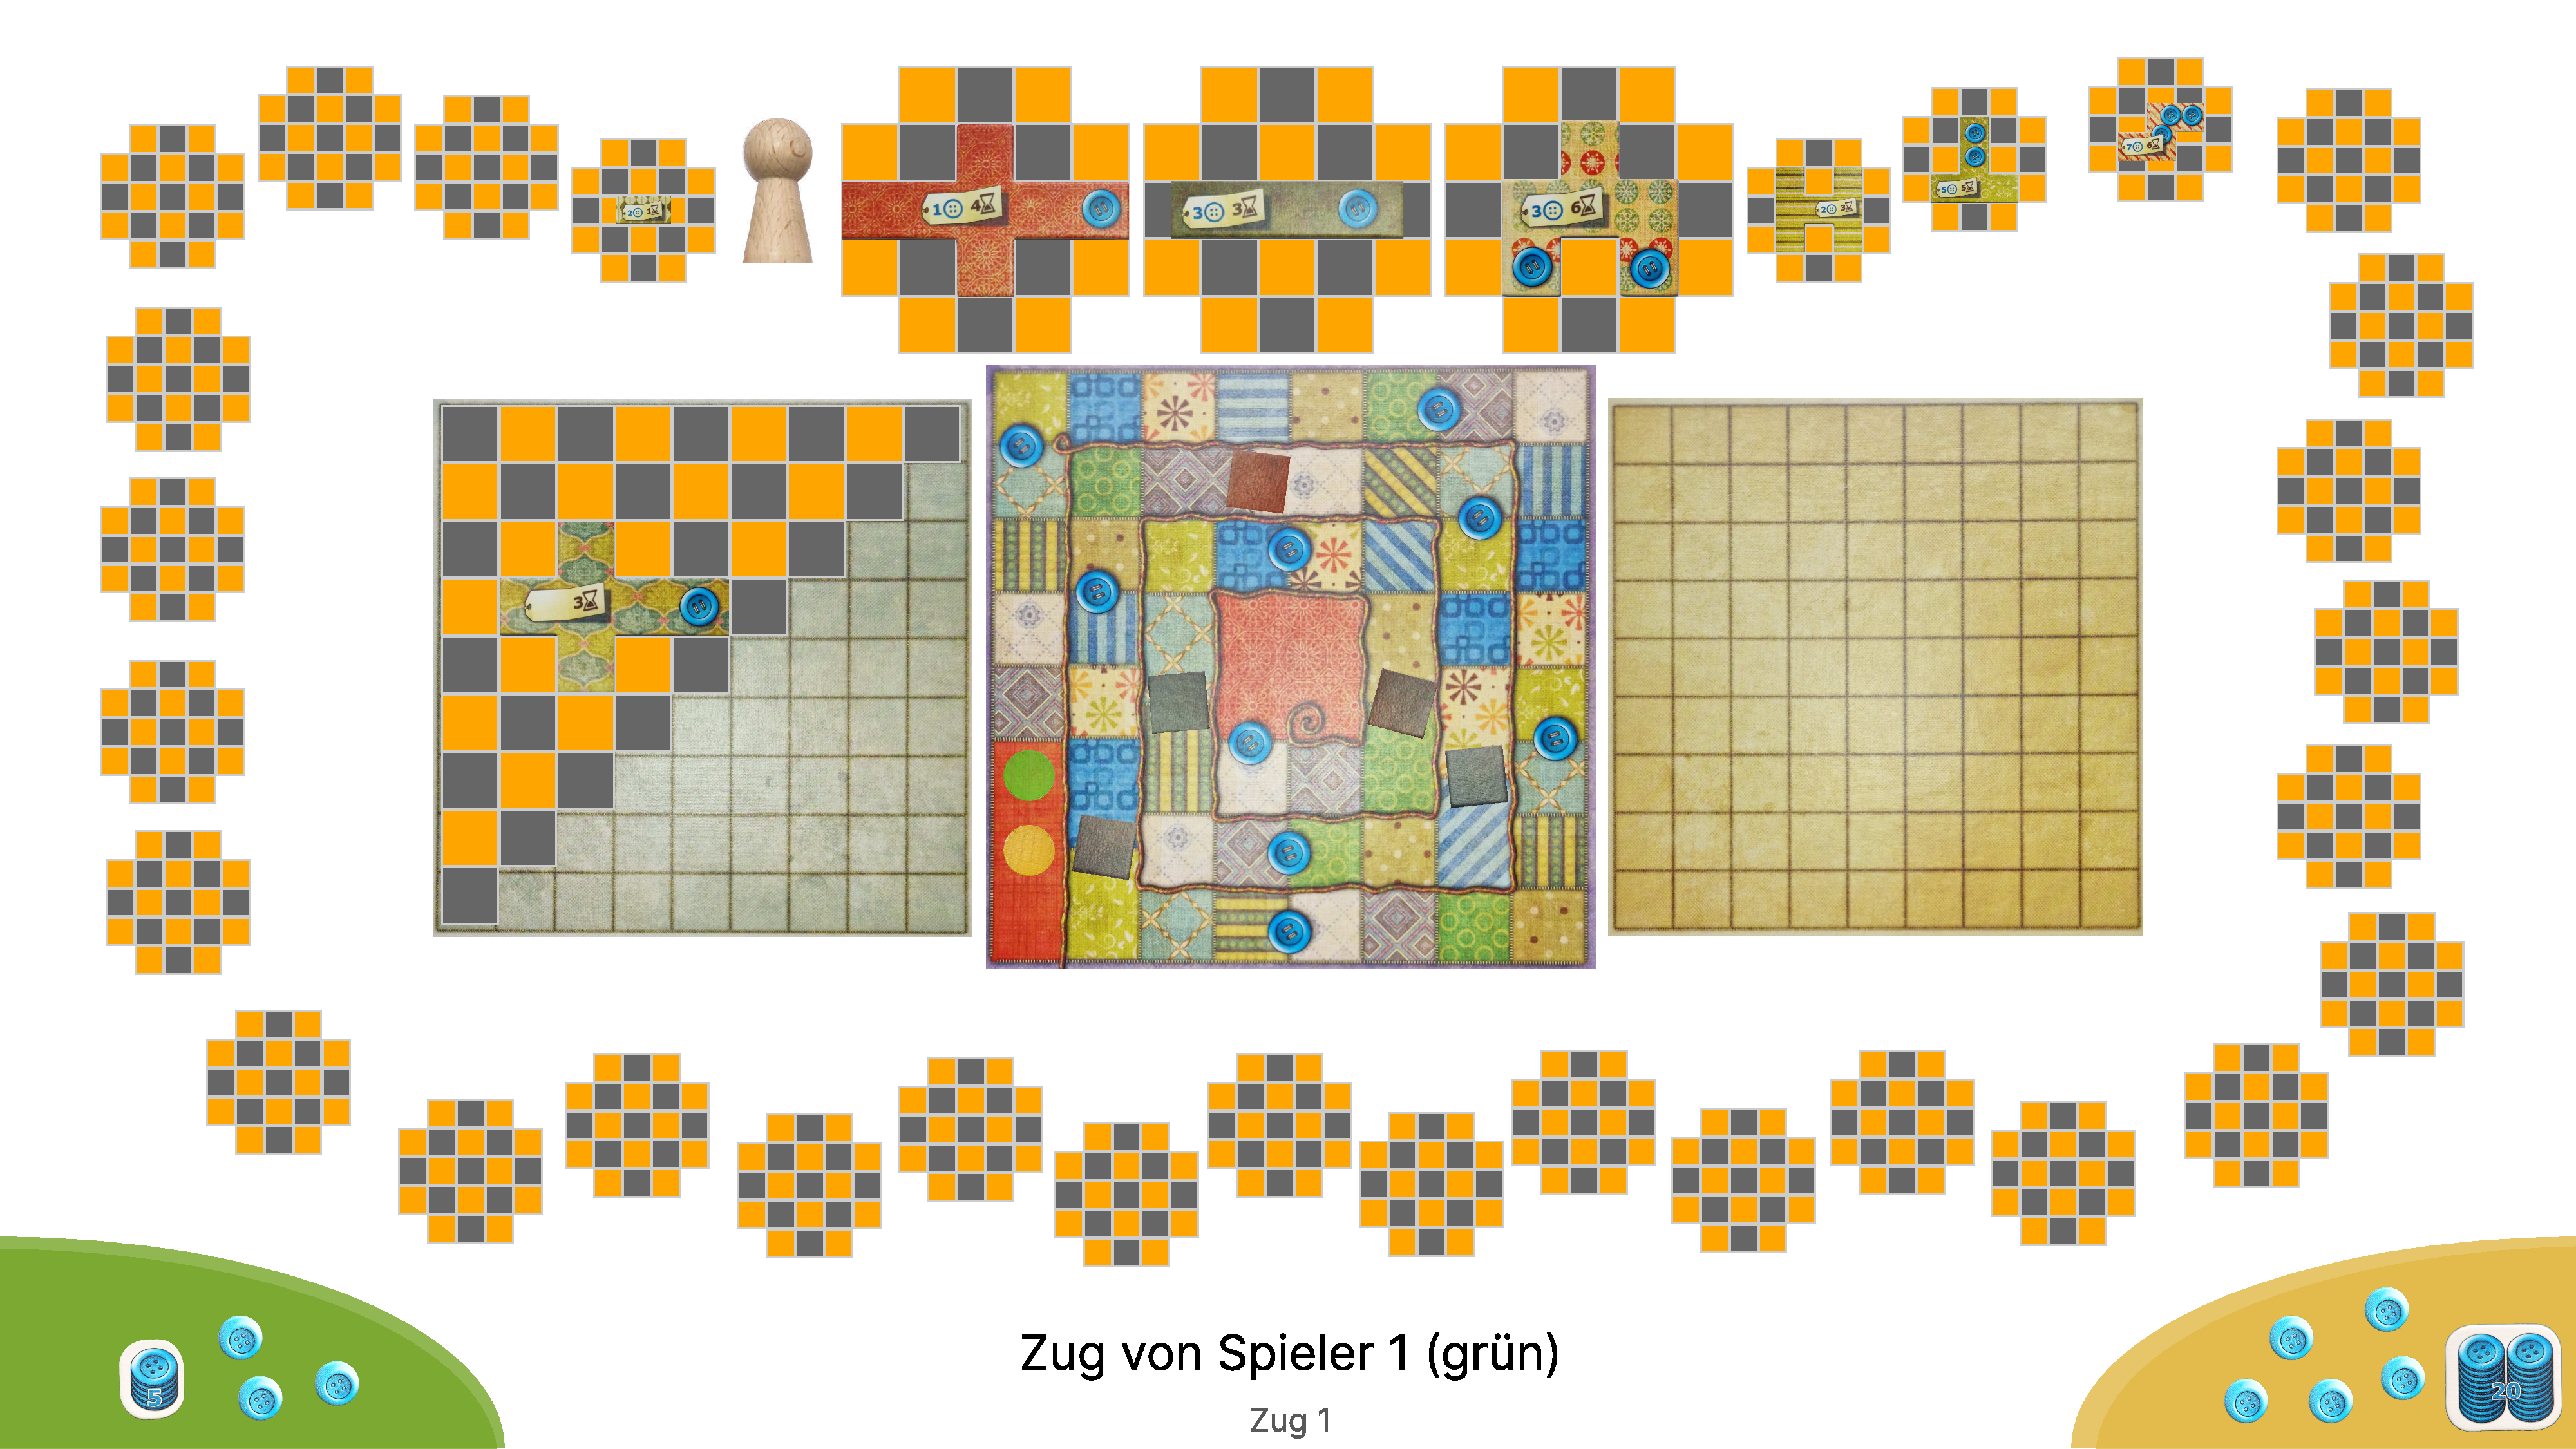
\includegraphics[width=\textwidth]{res/pictures/design_game_ui.pdf}};
        \drawshadow{image}
    \end{tikzpicture}}
    \caption{Designentwurf der grafische Benutzeroberfläche des Computerspiel}
    \label{fig:design-game-ui}
\end{figure}

Um das Brettspiel samt Spielgefühl bestmöglich auf das digitale Medium zu übertragen, wurde sich für das Design der Spieloberfäche, welche in der Abbildung \ref{fig:design-game-ui} zu sehen ist, am Spielaufbau des Brettspiels orientiert. Der Zeitplan liegt zentral in der Mitte der Oberfläche und wird an den Seiten von den Ablageplänen der beiden Spieler ergänzt.

Das Gesetz der Gleichheit bezüglich Farbe ausnutzend sind ist die Information, wie viel Knopfguthaben die Spieler haben, in den unteren Ecken der Oberfläche dargestellt. Um die Spielbretter herum sollen alle im Spiel befindlichen Flicken dargestellt werden, beziehungsweise in diesem Design die Platzhalter für diese Flicken. Hierbei sind die vom Spieler auswählbaren Flicken in voller Größe dargestellt, um sie hervorzuheben. Um diesen Aspekt zu erzielen, wird an dieser Stelle ebenfalls das Gesetz der Gleichheit, sowie das Gesetz der Nähe angewandt. Das letzte Gesetz wird hier außerdem dazu verwendet, um die Knöpfe zum Spiegeln und Rotieren der Flicken dem jeweiligen Flicken eindeutig zuzuordnen. 

Insgesamt wurde bei der Darstellung aller Flicken die Gesetze der Nähe und der Ähnlichkeit verwendet: Alle Flicken zusammen wirken durch ihre räumliche Nähe als eine Einheit, während die Unterscheidung zwischen wählbar und nicht wählbar durch die Größe dargestellt wird. Durch die kleine Darstellung der nicht auswählbaren Flicken wird dieses Constraints dem Spieler grafisch vermittelt. Das Wirken als Einheit soll sich bei dem Platzieren eines Flickens, beziehungsweise dem Wechsel der auswählbaren Flicken, durch die Gesetze der Gleichzeitigkeit und der gemeinsamen Bewegung noch verstärkt werden. So soll die Flickeneinheit sich als Kreis drehen, bis die als nächstes auswählbaren Flicken an der richtigen Position in der oberen Mitte der Oberfläche angekommen sind. Dies muss durch eine langsame Transformation der Flicken passieren, damit diese Bewegung von deutlich mehr als fünf Objekten noch korrekt interpretiert werden kann. Die Interpretation dieser Bewegung sollte durch die ständige Wiederholung derselben, jedoch nach gewisser Zeit den Spielern sehr leichtfallen, was allerdings noch durch Spielerbefragungen verifiziert werden sollte. 

Bei der Platzierung der Flicken soll auf das dem Benutzer durch zahlreiche andere Anwendungen bekannte Drag-and-Drop zur direkten Manipulation der Flicken zurückgegriffen werden. Dazu soll der transformierte Flicken mittels Mausklick ausgewählt werden können und wie im physischen Spiel auch zum eigenen Ablageplan bewegt werden und platziert werden können. Dasselbe Verfahren soll auch bei einer gewünschten Laufaktion des Spielers verwendet werden, was bedeutet, dass der Spieler einfach seine Spielfigur auf das korrekte Feld auf dem Zeitplan stellen muss, um die Aktion auszuführen, wodurch sich das Computerspiel wie die Vorlage spielt, eine Kenntnisübertragung möglich ist und ein ähnliches Spielgefühl entstehen kann. 

\pagebreak

Unten in der Mitte sind die aktuellen Statusinformationen über das Spiel abgebildet, dort soll allerdings auch Spielbenachrichtigungen platzfinden, wie zum Beispiel der Aufforderung zur Platzierung des Spezialflickens, um die Einstiegshürde für neue Spieler weiter zu senken.

\begin{figure}[!ht]
    \centering
    \resizebox{\textwidth}{!}{\begin{tikzpicture}
        \node [inner sep=0pt,,outer sep=0pt,clip,rounded corners=0.15cm] (image) at (0,0) {
            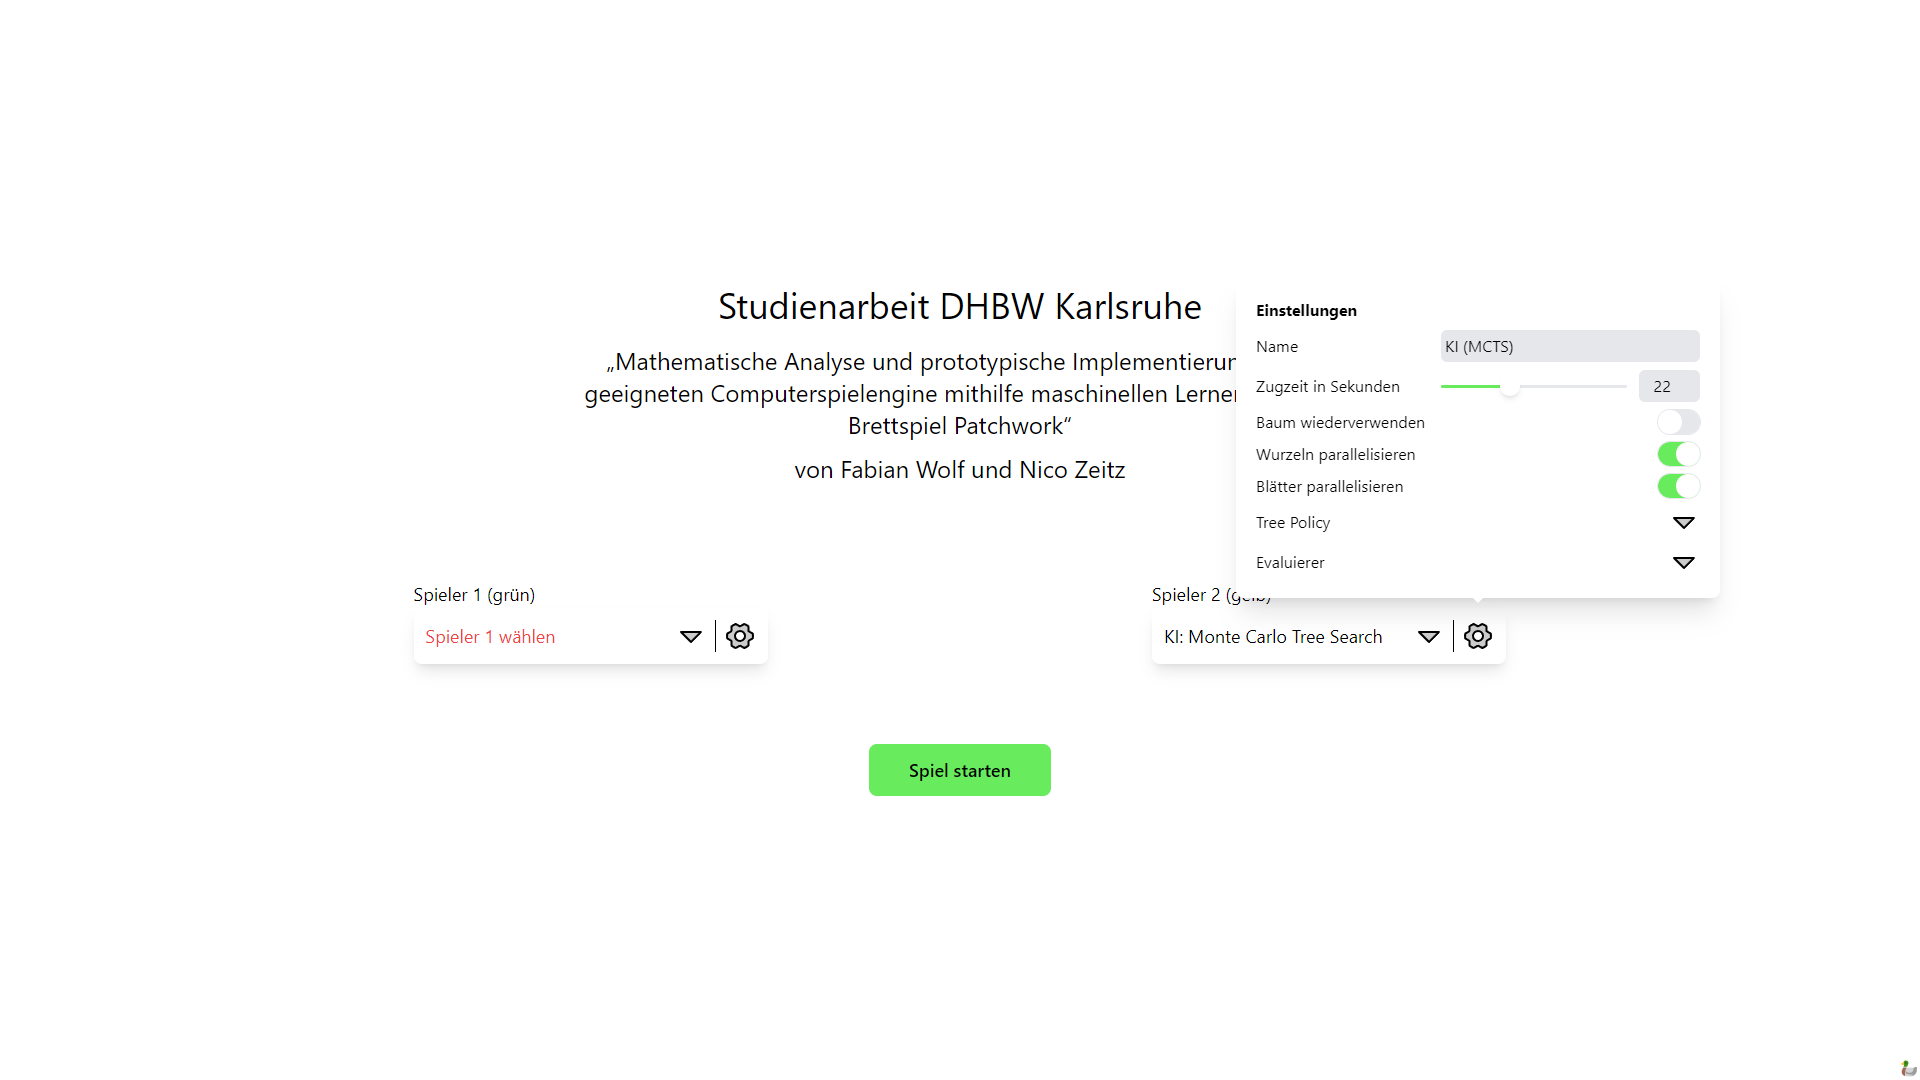
\includegraphics[width=\textwidth]{res/pictures/final_main_ui.png}};
        \drawshadow{image}
    \end{tikzpicture}}
    \caption{Umsetzung des Hauptmenüs des Computerspiel}
    \label{fig:final-main-ui}
\end{figure}

Bei Betrachtung der Umsetzung des Hauptmenüs in Abbildung \ref{fig:final-main-ui} im Vergleich zum Design in Abbildung \ref{fig:final-main-ui} lässt sich kein großer grafischer Unterschied feststellen. Das aufgeklappte Einstellungsmenü für die Computerspielengine \ac{MCTS}, verwendet bekannte Muster und Analogien zu Modifikation der Engine, wie zum Beispiel einem Slider zur annäherungsweisen Eingabe der Zugzeit der Engine, durch das Eingabefeld für genauere Eingabe erweitert. Diese Benutzeroberfläche des Hauptmenüs lässt sich laut ersten Testern intuitiv bedienen und wird als selbsterklärend beschrieben.

\pagebreak

\begin{figure}[!ht]
    \centering
    \resizebox{\textwidth}{!}{\begin{tikzpicture}
        \node [inner sep=0pt,,outer sep=0pt,clip,rounded corners=0.15cm] (image) at (0,0) {
            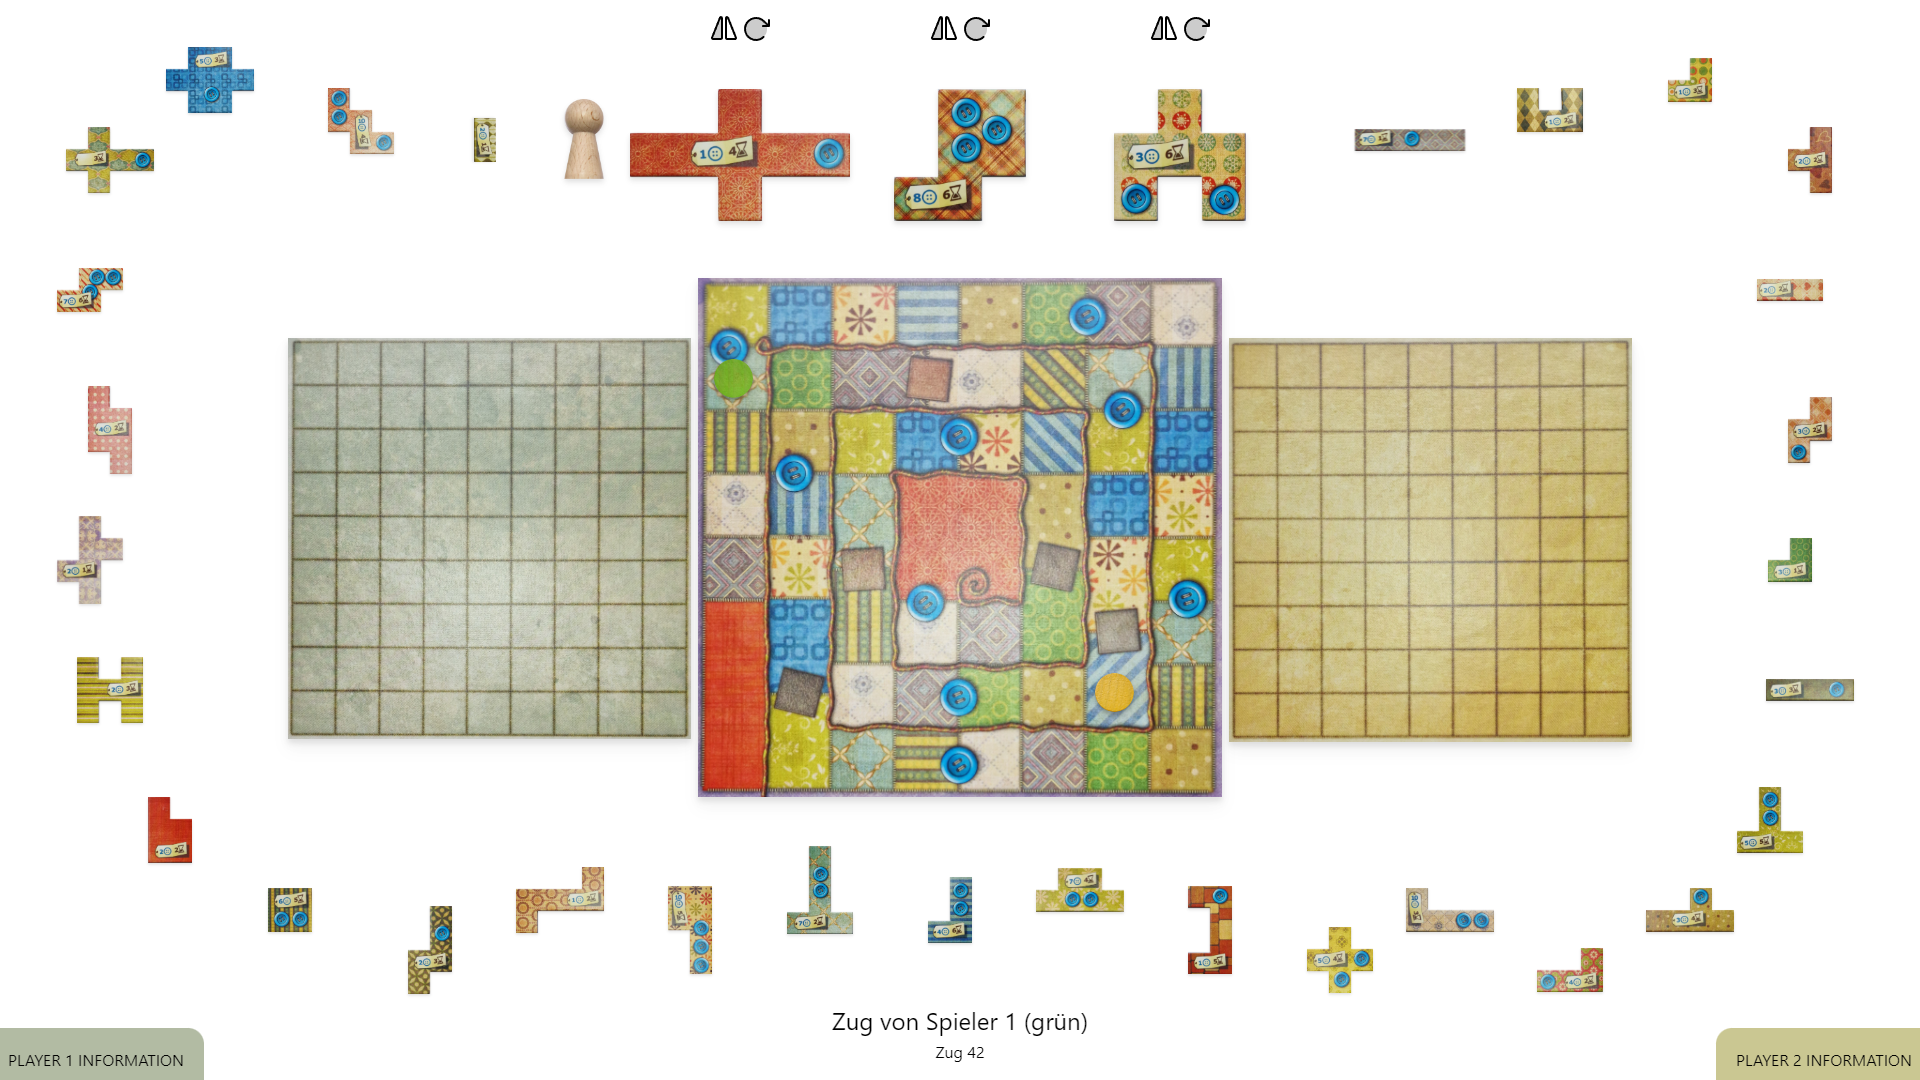
\includegraphics[width=\textwidth]{res/pictures/final_game_ui.png}};
        \drawshadow{image}
    \end{tikzpicture}}
    \caption{Umsetzung der grafische Benutzeroberfläche des Computerspiel}
    \label{fig:final-game-ui}
\end{figure}

Ebenso ist in der Umsetzung der Benutzeroberfläche des Computerspiels, in Abbildung \ref{fig:final-game-ui} zu sehen, deutlich das ursprüngliche Design zu erkennen. Die Flicken wirken in Kombination wie eine Kette, welche sich um die Spielbretter im Inneren zieht und werden durchaus als eine Einheit wahrgenommen. Ebenso erfolgreich wirkt die Unterscheidung zwischen auswählbaren Flicken, welche sich in der korrekten Größe für die Platzierung auf dem Ablageplan befinden, während die kleinen Flicken mit der Hälfte der Größe die gewünschte Unerreichbarkeit gegenüber den Spielern ausstrahlen. Die Zuordnung von Spielerinformationen zu den Ablageplänen funktioniert durch die gleiche Farbe ebenso erfolgreich. An dieser Stelle wird teilweise offensichtlich, dass die interaktive Benutzeroberfläche noch nicht fertiggestellt erscheint, da aufgrund von Zeitmangel die Implementierung nicht vollendet werden konnte.
\chapter{Evaluation}
\label{chapter:evaluation}

% \definecolor{win}{HTML}{0de929}
% \definecolor{loss}{HTML}{ef4748}
\definecolor{win}{HTML}{63be7b}
\definecolor{loss}{HTML}{f8696b}

Nachfolgend wird eine Evaluation der einzelnen Computerengines vorgenommen. Dazu spielen die Computerengines erst einmal verschiedene Vergleichsspiele untereinander. Die Vergleichsspiele sind dabei alle auf einem System mit folgenden Spezifikationen ausgeführt worden:

\begin{itemize}
    \item \vspace{-0.15cm} \textbf{Prozessor:} \ac{AMD} Ryzen 7 5800X 8-Core Processor
    \item \vspace{-0.15cm} \textbf{Arbeitsspeicher:} 32 \acsp{GiB} @ 3600 \acsp{MHz}
    \item \vspace{-0.15cm} \textbf{Betriebssystem:} Windows 11
    \item \vspace{-0.15cm} \textbf{Rust Version:} rustc 1.77.2
\end{itemize}

Nachfolgend werden, sofern nicht anders beschrieben, immer 100 Vergleichsspiele zwischen 2 Spielern gegeneinander gespielt. Dabei hat jeder Spieler immer eine Bedenkzeit von $10\acs{s}$, um eine Aktion auszuwählen. Computerengines mit Parallelisierung stehen 8 Threads zur Verfügung.

Die Stichprobe von 100 Spielen ist zu klein, um verlässliche statistische Vorhersagen zu treffen, vor allem was die genauen Gewinnraten der Spieler gegeneinander betrifft. Eine Tendenz der Ergebnisse lässt sich aber dennoch feststellen. Die kleine Anzahl an Vergleichsspielen ergibt sich aus der zeitlichen und hardwaretechnischen Ressourcenbegrenzung. Ein Spieler hat $10\acs{s}$ Bedenkzeit, multipliziert mit der durchschnittlichen Anzahl an \hyperref[text:ply]{\emph{Plys}} ($42{,}8176$) und den 100 Vergleichsspielen, ergibt sich eine Zeit von ca. $11,89$ Stunden für ein Vergleich zwischen zwei Spielern. Hardwaretechnisch werden alle Spiele auf dem gleichen oben genannten Rechnersystem durchgeführt, um vergleichbare Ergebnisse zu erhalten. Somit war es nicht möglich für die Evaluation mehr Vergleichsspiele durchzuführen. Bei den Vergleichsspielen wird immer nur das Endergebnis (also Gewinnen oder Verlieren) betrachtet, nicht die genaue Endwertung. In tatsächlichen Spielen geht es auch darum welcher Spieler gewinnt und nicht mit welcher Punktzahl. Außerdem wird die genaue Endwertung stark durch die initiale Flickenverteilung, den Spielverlauf und das Gegnerverhalten bestimmt. Spielen zwei starke Spieler gegeneinander, kann die Endwertung niedriger ausfallen als bei zwei schwächeren Spielern, da sich die starken Spieler vielleicht auch gegenseitig die besten Aktionen verbauen.

\begin{figure}[!ht]
    \centering
    \resizebox{\textwidth}{!}{\begin{tikzpicture}
            \coordinate (bar1Start) at (0,0);
            \coordinate (bar1End) at (10,0);
            \coordinate (bar1Break) at (2.1,0);

            \draw[color=win, line width=0.25cm] (bar1Start) -- (bar1Break);
            \draw[color=loss, line width=0.25cm] (bar1Break) -- (bar1End);
            \node[left = 0.1cm of bar1Start] {Random Player};
            \node[right = 0.1cm of bar1End, align=left] {Greedy Player \\ (eval: static)};
            \node[above right = 0.05cm and -0.15cm of bar1Start] {\footnotesize $21$ Gewonnen};
            \node[below = 0.1cm of bar1Break] {\scriptsize $21\%$};
            \node[above left = 0.05cm and -0.15cm of bar1End] {\footnotesize $79$ Verloren};
        \end{tikzpicture}}
    % \vspace*{-0.5cm}
    \caption{Random Player vs. Greedy Player}
    \label{fig:random-greedy-comparison}
\end{figure}

Die Evaluation beginnt mit einem einfachen Vergleich zwischen dem Random Spieler und dem Greedy Spieler mit dem statischen Evaluator. Die Ergebnisse der Vergleichsspiele sind in Abbildung \ref{fig:random-greedy-comparison} dargestellt. Wie zu erwarten, schneidet der Random Spieler schlechter ab als der Greedy Spieler mit 21 Gewonnenen und 79 Verlorenen Spielen. Somit kann in allen nachfolgenden Vergleichen angenommen werden, dass der Random Spieler eine Basis ist, die vermutlich jede andere Engine überwinden kann und der Greedy Player ein guter etwas anspruchsvollerer Vergleichspartner ist.

\section{Vergleich der PVS-Varianten}

Beim \ac{PVS} Spieler werden zuerst während der Suche typische Statistiken betrachtet. Die in Abbildung \ref{fig:pvs-statistics} gezeigten Werte stammen dabei aus einem tatsächlich stattgefundenen Spiel, sind aber vergleichbar mit in anderen Spielen beobachteten Werten.

% ┌───────────────────────────── Principal Variation Search Player ─────────────────────────────┐
% │ Features:            [AW, TT(S), LMR, LMP, SE]                                              │
% │ Depth:               9 started from (P1: 11, P2: 13, type: Normal)                            │
% │ Time:                5.0634892s                                                             │
% │ Nodes searched:      43720                                                                  │
% │ Branching factor:    2.84 AVG / 1.78 EFF / 1.38 MEAN                                        │
% │ Best Action:         P7I1═4‖3↻1↔0P1 (3 points)                                              │
% │ Move Ordering:       86.80\% (8611 high pv / 9920 high)                                      │
% │ Aspiration window:   0 low / 0 high                                                         │
% │ Zero window search:  2 fails (0.01\%)                                                        │
% │ Search Extensions:   1 SP, 0 ST (enabled)                                                   │
% │ LMR (Fail/All):      0/114 (0.00%)                                                          │
% │ LMP:                 3271                                                                   │
% │ Principal Variation: P7I1═4‖3↻1↔0P1 → P21I0═2‖1↻0↔0P0 → P31I0═7‖4↻0↔1P1 → P11I0═0‖2↻0↔1P0 │
% │ ┌──────────────────────────── Transposition Table Statistics ─────────────────────────────┐ │
% │ │ Capacity:            10416666                                                           │ │
% │ │ Entries:              5257801 /  50.47\% filled                                          │ │
% │ │ Overwrites:          13138704                                                           │ │
% │ │ Accesses:             1141676                                                           │ │
% │ │ ├──► Hit:              261862 /  22.94\%                                                 │ │
% │ │ └──► Miss:             879814 /  77.06\%                                                 │ │
% │ └─────────────────────────────────────────────────────────────────────────────────────────┘ │
% └─────────────────────────────────────────────────────────────────────────────────────────────┘
\begin{figure}[!ht]
    \centering
    \resizebox{\textwidth}{!}{\begin{tcolorbox}[
                rounded corners=all,
                boxrule=1pt,
                colback=white,
                colframe=black,
                hbox,
                % width=\linewidth,
                enhanced,
                coltitle=black,
                title={\acl{PVS} Player},
                top=6pt,
                left=0pt,
                right=5pt,
                bottom=0pt,
                attach boxed title to top center={yshift=-\tcboxedtitleheight/2},
                boxed title style={size=small,colback=white,colframe=white}
            ]
            \begingroup
            \setlength{\arrayrulewidth}{0pt}

            \begin{tabular}{@{}ll@{}}
                Features:             & [AW, TT(S), \acs{LMR}, \acs{LMP}, SE]                                \\
                Depth:                & $9$ started from (P1: $11$, P2: $13$, type: Normal)                  \\
                Time:                 & $5{,}0634892\acs{s}$                                                 \\
                Nodes searched:       & $43720$                                                              \\
                % Branching factor:   & $2{,}84$ AVG / $1{,}78$ EFF / $1{,}38$ MEAN                          \\
                Branching factor:     & $13{,}73$ AVG / $3{,}32$ EFF / $1{,}59$ MEAN                         \\
                Best Action:          & P7I1═4‖3↻1↔0P1 ($3$ points)                                          \\
                Action Ordering:      & $86{,}80\%$ ($8611$ high pv / $9920$ high)                           \\
                Aspiration window:    & $0$ low / $0$ high                                                   \\
                Zero window search:   & $2$ fails ($0{,}01\%$)                                               \\
                Search Extensions:    & $1$ SP, $0$ ST (enabled)                                             \\
                \acs{LMR} (Fail/All): & $0/114$ ($0{,}00\%$)                                                 \\
                \acs{LMP}:            & $3271$                                                               \\
                \acl{PV}:             & P7I1═4‖3↻1↔0P1 → P21I0═2‖1↻0↔0P0 → P31I0═7‖4↻0↔1P1 → P11I0═0‖2↻0↔1P0 \\
                \multicolumn{2}{@{}c@{}}{
                \begin{tcolorbox}[
                        rounded corners=all,
                        boxrule=1pt,
                        colback=white,
                        colframe=black,
                        width=1.325\linewidth,
                        enhanced,
                        coltitle=black,
                        title={Transposition Table},
                        top=6pt,
                        left=0pt,
                        right=0pt,
                        bottom=0pt,
                        attach boxed title to top center={yshift=-\tcboxedtitleheight/2},
                        boxed title style={size=small,colback=white,colframe=white}
                    ]
                    \begin{tabular}{ll}
                        Capacity:   & $10416666$                      \\
                        Entries:    & $5257801$ /  $50{,}47\%$ filled \\
                        Overwrites: & $13138704$                      \\
                        Accesses:   & $1141676$                       \\
                        ├──► Hit:   & $261862$ /  $22{,}94\%$         \\
                        └──► Miss:  & $879814$ /  $77{,}06\%$         \\
                    \end{tabular}
                \end{tcolorbox}
                }                                                                                            \\
            \end{tabular}
            \endgroup
        \end{tcolorbox}}
    \vspace*{-0.25cm}
    \caption[PVS-Suchstatistiken]{\acs{PVS}-Suchstatistiken}
    \label{fig:pvs-statistics}
\end{figure}

TODO:

\begin{figure}[!ht]
    \centering
    \resizebox{\textwidth}{!}{\begin{tikzpicture}
            % \coordinate (bar1Start) at (0,0);
            % \coordinate (bar1End) at (10,0);
            % \coordinate (bar1Break) at (6.4,0);

            % \draw[color=win, line width=0.25cm] (bar1Start) -- (bar1Break);
            % \draw[color=loss, line width=0.25cm] (bar1Break) -- (bar1End);
            % \node[left = 0.1cm of bar1Start] {Hard-Fail};
            % \node[right = 0.1cm of bar1End] {Soft-Fail};
            % \node[above right = 0.05cm and -0.15cm of bar1Start] {\footnotesize $64$ Gewonnen};
            % \node[below = 0.1cm of bar1Break] {\scriptsize $64\%$};
            % \node[above left = 0.05cm and -0.15cm of bar1End] {\footnotesize $36$ Verloren};

            \coordinate (bar2Start) at (0,0);
            \coordinate (bar2End) at (10,0);
            \coordinate (bar2Break) at (5.1,0);

            \draw[color=win, line width=0.25cm] (bar2Start) -- (bar2Break);
            \draw[color=loss, line width=0.25cm] (bar2Break) -- (bar2End);
            \node[left = 0.1cm of bar2Start] {AspirationWindow};
            \node[right = 0.1cm of bar2End] {Kein AspirationWindow};
            \node[above right = 0.05cm and -0.15cm of bar2Start] {\footnotesize $51$ Gewonnen};
            \node[below = 0.1cm of bar2Break] {\scriptsize $51\%$};
            \node[above left = 0.05cm and -0.15cm of bar2End] {\footnotesize $49$ Verloren};

            \coordinate (bar3Start) at (0,-1.5);
            \coordinate (bar3End) at (10,-1.5);
            \coordinate (bar3Break) at (5.4,-1.5);

            \draw[color=win, line width=0.25cm] (bar3Start) -- (bar3Break);
            \draw[color=loss, line width=0.25cm] (bar3Break) -- (bar3End);
            \node[left = 0.1cm of bar3Start] {Sucherweiterungen};
            \node[right = 0.1cm of bar3End] {Keine Sucherweiterungen};
            \node[above right = 0.05cm and -0.15cm of bar3Start] {\footnotesize $54$ Gewonnen};
            \node[below = 0.1cm of bar3Break] {\scriptsize $54\%$};
            \node[above left = 0.05cm and -0.15cm of bar3End] {\footnotesize $46$ Verloren};

            \coordinate (bar4Start) at (0,-3);
            \coordinate (bar4End) at (10,-3);
            \coordinate (bar4Break) at (5.3,-3);

            \draw[color=win, line width=0.25cm] (bar4Start) -- (bar4Break);
            \draw[color=loss, line width=0.25cm] (bar4Break) -- (bar4End);
            \node[left = 0.1cm of bar4Start] {\acs{LMR}, \acs{LMP}};
            \node[right = 0.1cm of bar4End] {Kein \acs{LMR}, \acs{LMP}};
            \node[above right = 0.05cm and -0.15cm of bar4Start] {\footnotesize $53$ Gewonnen};
            \node[below = 0.1cm of bar4Break] {\scriptsize $53\%$};
            \node[above left = 0.05cm and -0.15cm of bar4End] {\footnotesize $47$ Verloren};

            \coordinate (bar5Start) at (0,-4.5);
            \coordinate (bar5End) at (10,-4.5);
            \coordinate (bar5Break) at (5,-4.5);

            \draw[color=win, line width=0.25cm] (bar5Start) -- (bar5Break);
            \draw[color=loss, line width=0.25cm] (bar5Break) -- (bar5End);
            \node[left = 0.1cm of bar5Start] {Table Ordering};
            \node[right = 0.1cm of bar5End] {Static Eval Ordering};
            \node[above right = 0.05cm and -0.15cm of bar5Start] {\footnotesize $50$ Gewonnen};
            \node[below = 0.1cm of bar5Break] {\scriptsize $50\%$};
            \node[above left = 0.05cm and -0.15cm of bar5End] {\footnotesize $50$ Verloren};

            \coordinate (bar6Start) at (0,-6);
            \coordinate (bar6End) at (10,-6);
            \coordinate (bar6Break) at (4.1,-6);

            \draw[color=win, line width=0.25cm] (bar6Start) -- (bar6Break);
            \draw[color=loss, line width=0.25cm] (bar6Break) -- (bar6End);
            \node[left = 0.1cm of bar6Start] {Kein \acs{SMP}};
            \node[right = 0.1cm of bar6End] {Lazy \acs{SMP}};
            \node[above right = 0.05cm and -0.15cm of bar6Start] {\footnotesize $41$ Gewonnen};
            \node[below = 0.1cm of bar6Break] {\scriptsize $41\%$};
            \node[above left = 0.05cm and -0.15cm of bar6End] {\footnotesize $59$ Verloren};
        \end{tikzpicture}}
    % \vspace*{-0.5cm}
    \caption[Vergleich der PVS Varianten]{Vergleich der \acs{PVS} Varianten}
    \label{fig:pvs-comparision}
\end{figure}

TODO:

\pagebreak

\section{Vergleich der MCTS-Varianten}

Im diesen Abschnitt werden die einzelnen Varianten des \ac{MCTS} Spielers miteinander verglichen. Zuerst sind dabei alle Tree Policies sowie Evaluatoren in der Tabelle \ref{tabelle:mcts-policy-eval-comparision} aufgelistet. Dabei tritt jede Kombination gegen jede andere Kombination an. In den einzelnen Zellen ist das Ergebnis der Vergleichsspiele als Gewinnrate zwischen 0 und 1 aus Sicht des Zeilenspielers aufgetragen (So gewinnt beispielsweise \emph{\acs{UCT},Win} mit $56{,}2\%$ gegen \emph{\acs{UCT},Score}). Die Vergleichsspiele umfassen dabei immer 1000 Spiele mit je 2500 Iterationen pro \hyperref[text:ply]{\emph{Ply}}. Um möglichst vergleichbare Spiele sicherzustellen, werden keine Suchbäume wiederverwendet und es findet auch keine Parallelisierung der einzelnen \ac{MCTS} Varianten statt.

\begin{table}[H]
    \centering
    \resizebox{\textwidth}{!}{\begin{tabular}{|c|c|c|c|c|c|c|c|c|c|c|}
            \hline
            \multicolumn{1}{|c}{Policy}       & $\rightarrow$ & \ac{UCT}                          & \ac{UCT}                          & \ac{UCT}                          & Score                             & Score                             & Score                             & \tiny \makecell{Partial-                                                                                  \\Score}  & \tiny \makecell{Partial-\\Score}  & \tiny \makecell{Partial-\\Score}  \\ \cline{3-11}
            \multicolumn{1}{|c}{$\downarrow$} & Evaluator     & Win                               & Score                             & Static                            & Win                               & Score                             & Static                            & Win                               & Score                             & Static                            \\ \hline
            \ac{UCT}                          & Win           & $\diagup$                         & \cellcolor[HTML]{ece683}$0{,}562$ & \cellcolor[HTML]{67bf7c}$0{,}989$ & \cellcolor[HTML]{c5db81}$0{,}686$ & \cellcolor[HTML]{fee883}$0{,}490$ & \cellcolor[HTML]{85c87d}$0{,}894$ & \cellcolor[HTML]{f3e884}$0{,}541$ & \cellcolor[HTML]{f7e984}$0{,}526$ & \cellcolor[HTML]{82c77d}$0{,}902$ \\ \hline
            \ac{UCT}                          & Score         & \cellcolor[HTML]{feda80}$0{,}438$ & $\diagup$                         & \cellcolor[HTML]{68c07c}$0{,}984$ & \cellcolor[HTML]{cadc81}$0{,}673$ & \cellcolor[HTML]{fbea84}$0{,}516$ & \cellcolor[HTML]{7ec67d}$0{,}914$ & \cellcolor[HTML]{f7e984}$0{,}526$ & \cellcolor[HTML]{feea83}$0{,}499$ & \cellcolor[HTML]{85c87d}$0{,}894$ \\ \hline
            \ac{UCT}                          & Static        & \cellcolor[HTML]{f86b6b}$0{,}011$ & \cellcolor[HTML]{f86d6b}$0{,}016$ & $\diagup$                         & \cellcolor[HTML]{f8726c}$0{,}038$ & \cellcolor[HTML]{f86d6b}$0{,}018$ & \cellcolor[HTML]{fcb87a}$0{,}305$ & \cellcolor[HTML]{f86e6c}$0{,}021$ & \cellcolor[HTML]{f86c6b}$0{,}013$ & \cellcolor[HTML]{fcb87a}$0{,}304$ \\ \hline
            Score                             & Win           & \cellcolor[HTML]{fcba7a}$0{,}314$ & \cellcolor[HTML]{fcbe7b}$0{,}327$ & \cellcolor[HTML]{6fc27c}$0{,}962$ & $\diagup$                         & \cellcolor[HTML]{fdca7d}$0{,}374$ & \cellcolor[HTML]{a0d07f}$0{,}805$ & \cellcolor[HTML]{fcc07b}$0{,}335$ & \cellcolor[HTML]{fcc47c}$0{,}353$ & \cellcolor[HTML]{9dcf7f}$0{,}816$ \\ \hline
            Score                             & Score         & \cellcolor[HTML]{fceb84}$0{,}510$ & \cellcolor[HTML]{fee683}$0{,}484$ & \cellcolor[HTML]{69c07c}$0{,}982$ & \cellcolor[HTML]{d8e082}$0{,}626$ & $\diagup$                         & \cellcolor[HTML]{7ec67d}$0{,}915$ & \cellcolor[HTML]{f6e984}$0{,}531$ & \cellcolor[HTML]{fbea84}$0{,}516$ & \cellcolor[HTML]{80c77d}$0{,}909$ \\ \hline
            Score                             & Static        & \cellcolor[HTML]{f98470}$0{,}106$ & \cellcolor[HTML]{f97f6f}$0{,}086$ & \cellcolor[HTML]{c3da81}$0{,}695$ & \cellcolor[HTML]{fa9b74}$0{,}195$ & \cellcolor[HTML]{f97f6f}$0{,}085$ & $\diagup$                         & \cellcolor[HTML]{f98871}$0{,}123$ & \cellcolor[HTML]{f9806f}$0{,}092$ & \cellcolor[HTML]{fedf81}$0{,}457$ \\ \hline
            \tiny \makecell{Partial-                                                                                                                                                                                                                                                                                                                                                              \\Score} &           Win & \cellcolor[HTML]{fee081}$0{,}459$ & \cellcolor[HTML]{fee482}$0{,}474$ & \cellcolor[HTML]{6ac07c}$0{,}979$ & \cellcolor[HTML]{ccdd82}$0{,}665$ & \cellcolor[HTML]{fee282}$0{,}469$ & \cellcolor[HTML]{8aca7e}$0{,}877$ & $\diagup$                         & \cellcolor[HTML]{fbea84}$0{,}513$ & \cellcolor[HTML]{82c77d}$0{,}903$ \\ \hline
            \tiny \makecell{Partial-                                                                                                                                                                                                                                                                                                                                                              \\Score} &         Score & \cellcolor[HTML]{fee482}$0{,}474$ & \cellcolor[HTML]{ffeb84}$0{,}501$ & \cellcolor[HTML]{68c07c}$0{,}987$ & \cellcolor[HTML]{d2de82}$0{,}647$ & \cellcolor[HTML]{fee683}$0{,}484$ & \cellcolor[HTML]{80c77d}$0{,}908$ & \cellcolor[HTML]{fee783}$0{,}487$ & $\diagup$                         & \cellcolor[HTML]{7cc67d}$0{,}920$ \\ \hline
            \tiny \makecell{Partial-                                                                                                                                                                                                                                                                                                                                                              \\Score} &        Static & \cellcolor[HTML]{f9826f}$0{,}098$ & \cellcolor[HTML]{f98470}$0{,}106$ & \cellcolor[HTML]{c2da81}$0{,}696$ & \cellcolor[HTML]{fa9874}$0{,}184$ & \cellcolor[HTML]{f9806f}$0{,}091$ & \cellcolor[HTML]{f2e884}$0{,}543$ & \cellcolor[HTML]{f9826f}$0{,}097$ & \cellcolor[HTML]{f97d6e}$0{,}080$ & $\diagup$                         \\ \hline
        \end{tabular}}
    \vspace{3pt}
    \caption{Vergleich der \acs{MCTS} Policy und Evaluator Varianten}
    \label{tabelle:mcts-policy-eval-comparision}
\end{table}

Wie in Tabelle \ref{tabelle:mcts-policy-eval-comparision} zu sehen ist, sind viele der Varianten sehr vergleichbar. So gewinnt die \emph{\acs{UCT},Win} Variante beispielsweise gegen alle anderen Varianten außer \emph{Score,Score}. Die \emph{Score,Score} Variante hingegen verliert gegen die \emph{\acs{UCT},Score} Variante, die wiederrum gegen die \emph{\acs{UCT},Win} Variante verliert. Die einzigen Varianten, welche eine deutlich schlechtere Leistung erbringen ist \emph{Score,Win} und alle Varianten mit dem statischen Evaluator. Die \emph{Score,Win} Variante erzeugt innerhalb der Simulationsphase immer das Ergebnis $-1$ oder $1$. Auf Basis dieser zwei Werte erzeugt die Score-Tree-Policy eine Auswahl der Knoten innerhalb der Selektionsphase, was natürlich nicht sehr aussagekräftig ist, womit auch das schlechtere Abschneiden erklärt ist. Die statische Evaluation wurde nur eingesetzt, weil es möglich ist. Jedoch wiederspricht diese statische Evaluation gerade dem Prinzip, wodurch der \ac{MCTS} Spieler seine Stärke erreicht: Möglichst viele Iterationen durchführen, um somit den wahren Wert einer Aktion durch eine genügend große Stichprobe an Spielverläufen ausreichend gut zu approximieren. Der statische Evaluator bricht den Vorgang verführt ab, um die Stichproben durch eine immer gleichbleibende und verzerrte Evaluation zu ersetzen. Somit ähnelt diese Variante eher dem \ac{PVS} Spieler der nur ein paar Ebenen tief schauen kann und schneidet deutlich schlechter ab, als die tatsächlichen \ac{MCTS} Varianten. Die tatsächlichen Varianten sind aber recht ähnlich. Aus diesem Grund wurde die \emph{Partial-Score} Tree Policy auch nur einmal mit $\rho = 10\%$ in die Tabelle mit aufgenommen. Nachfolgend wird deshalb auch einfach zufällig die \emph{\acs{UCT},WIn} Variante für die Vergleiche weiterverwendet .

\begin{figure}[!ht]
    \centering
    \begin{tikzpicture}
        \node at (5,0) [align=center] {$5{.}000$ Iterationen mit $2\acs{ms}$ Tree Reuse Timeout};

        \coordinate (bar1Start) at (0,-1);
        \coordinate (bar1End) at (10,-1);
        \coordinate (bar1Break) at (5,-1);

        \draw[color=win, line width=0.25cm] (bar1Start) -- (bar1Break);
        \draw[color=loss, line width=0.25cm] (bar1Break) -- (bar1End);
        \node[left = 0.1cm of bar1Start] {Tree New};
        \node[right = 0.1cm of bar1End] {Tree Reuse};
        \node[above right = 0.05cm and -0.15cm of bar1Start] {\footnotesize $500$ Gewonnen};
        \node[below = 0.1cm of bar1Break] {\scriptsize $50\%$};
        \node[above left = 0.05cm and -0.15cm of bar1End] {\footnotesize $500$ Verloren};

        \node at (5,-2.25) [align=center] {$100{.}000$ Iterationen};

        \coordinate (bar2Start) at (0,-3);
        \coordinate (bar2End) at (10,-3);
        \coordinate (bar2Break) at (4.99,-3);

        \draw[color=win, line width=0.25cm] (bar2Start) -- (bar2Break);
        \draw[color=loss, line width=0.25cm] (bar2Break) -- (bar2End);
        \node[left = 0.1cm of bar2Start] {Tree New};
        \node[right = 0.1cm of bar2End] {Tree Reuse};
        \node[above right = 0.05cm and -0.15cm of bar2Start] {\footnotesize $499$ Gewonnen};
        \node[below = 0.1cm of bar2Break] {\scriptsize $49{,}9\%$};
        \node[above left = 0.05cm and -0.15cm of bar2End] {\footnotesize $501$ Verloren};
    \end{tikzpicture}
    % \vspace*{-0.5cm}
    \caption[Vergleich Baumwiederverwendung bei MCTS]{Vergleich neuer Baum vs. Baum wiederverwenden bei \acs{MCTS}}
    \label{fig:mcts-tree-reuse-comparision}
\end{figure}

Weiterhin werden die \ac{MCTS} Spielervarianten noch verglichen, indem ein Spieler immer wieder versucht den alten Suchbaum wiederzuverwenden (\emph{Tree Reuse}), während der andere Spieler einfach direkt mit einem neuen Suchbaum anfängt (\emph{Tree New}). Die in \ref{fig:mcts-tree-reuse-comparision} gezeigten Ergebnisse sind dabei relative ernüchternd. Einerseits werden beide Varianten mit $5{.}000$ Iterationen getestet, wobei für \emph{Tree Reuse} ein Timeout von $2\acsp{ms}$ hat, um den neuen Spielzustand im alten Suchbaum zu finden. Andererseits werden beide Varianten noch mit je $100{.}000$ Iterationen pro \hyperref[text:ply]{\emph{Ply}} und keinem Timeout für \emph{Tree Reuse} verglichen. Beide Vergleiche enden dabei mit einer Gewinnrate von ziemlich genau $50\%$. Selbst bei Variante mit vielen Iterationen, bei der immer der Suchbaum wiederverwendet wird, gewinnt \emph{Tree Reuse} nur ein Spiel mehr, was statistisch wenig aussagekräftig ist. Dies ist der Fall, obwohl mehr Iterationen einen größeren Suchbaum und somit auch einen größeren wiederverwendeten Teilbaum implizieren. Wenn das Wiederverwenden des Suchbaums also einen Vorteil bringen sollte, dann ist der Versuchsaufbau oder die Stichprobengröße nicht groß genug, um diesen Vorteil eindeutig abzugrenzen.

\begin{figure}[!ht]
    \centering
    \begin{tikzpicture}
        \coordinate (bar1Start) at (0,0);
        \coordinate (bar1End) at (10,0);
        \coordinate (bar1Break) at (7.7,0);

        \draw[color=win, line width=0.25cm] (bar1Start) -- (bar1Break);
        \draw[color=loss, line width=0.25cm] (bar1Break) -- (bar1End);
        \node[left = 0.1cm of bar1Start, align=right] {\acs{MCTS}\\(1 Thread)};
        \node[right = 0.1cm of bar1End, align=left] {\acs{MCTS}\\(8 Leaf)};
        \node[above right = 0.05cm and -0.15cm of bar1Start] {\footnotesize $77$ Gewonnen};
        \node[below = 0.1cm of bar1Break] {\scriptsize $77\%$};
        \node[above left = 0.05cm and -0.15cm of bar1End] {\footnotesize $23$ Verloren};

        \coordinate (bar2Start) at (0,-1.5);
        \coordinate (bar2End) at (10,-1.5);
        \coordinate (bar2Break) at (4.6,-1.5);

        \draw[color=win, line width=0.25cm] (bar2Start) -- (bar2Break);
        \draw[color=loss, line width=0.25cm] (bar2Break) -- (bar2End);
        \node[left = 0.1cm of bar2Start, align=right] {\acs{MCTS}\\(1 Thread)};
        \node[right = 0.1cm of bar2End, align=left] {\acs{MCTS}\\(8 Root)};
        \node[above right = 0.05cm and -0.15cm of bar2Start] {\footnotesize $46$ Gewonnen};
        \node[below = 0.1cm of bar2Break] {\scriptsize $46\%$};
        \node[above left = 0.05cm and -0.15cm of bar2End] {\footnotesize $54$ Verloren};

        \coordinate (bar3Start) at (0,-3);
        \coordinate (bar3End) at (10,-3);
        \coordinate (bar3Break) at (1.8,-3);

        \draw[color=win, line width=0.25cm] (bar3Start) -- (bar3Break);
        \draw[color=loss, line width=0.25cm] (bar3Break) -- (bar3End);
        \node[left = 0.1cm of bar3Start, align=right] {\acs{MCTS}\\(8 Leaf)};
        \node[right = 0.1cm of bar3End, align=left] {\acs{MCTS}\\(8 Root)};
        \node[above right = 0.05cm and -0.15cm of bar3Start] {\footnotesize $18$ Gewonnen};
        \node[below = 0.1cm of bar3Break] {\scriptsize $18\%$};
        \node[above left = 0.05cm and -0.15cm of bar3End] {\footnotesize $82$ Verloren};
    \end{tikzpicture}
    % \vspace*{-0.5cm}
    \caption[Vergleich der MCTS Varianten]{Vergleich der \acs{MCTS} Varianten}
    \label{fig:mcts-comparision}
\end{figure}

Um die \ac{MCTS} Spielervergleiche abzuschließen, werden zuletzt die einzelnen Parallelisierungsmöglichkeiten untereinander in \ref{fig:mcts-comparision} verglichen. Dabei spielen die nicht parallelisierte Single-Threaded Variante sowie die Leaf- und Root-Parallelisierten Varianten mit 8 Threads gegenaeinander. Die \hyperref[text:leaf-parallelization]{\emph{Leaf Parallelisierung}} schneidet dabei am schlechtesten ab, auch schlechter als die \ac{MCTS} Suche mit einem Thread. Da der \ac{MCTS} Spieler in Patchwork generell sehr wenige Iterationen schafft, ist es wahrscheinlich besser die Change einen guten Spielverlauf zu finden durch viele Iterationen zu maximieren, anstatt weniger Pfade auszuprobieren und für diese Pfade mittels \hyperref[text:leaf-parallelization]{\emph{Leaf Parallelisierung}} eine etwas genaueren Schätzer für den tatsächlichen Wert eines Knotens zu erhalten. Am besten spielt die \hyperref[text:root-parallelization]{\emph{Root-Parallelisierte}} Variante. Diese setzt sich gegen beide anderen Varianten durch, auch wenn der Vorsprung vor der Single-Threaded Variante geringer ausfällt als erhofft.

% ┌───────────────────────────── MCTS Player ─────────────────────────────┐
% │ Features:            [RP(8), RT]                                      │
% │ Duration:            9.925s                                           │
% │ Total Iterations:    592082                                           │
% │ Iterations:          74767                                            │
% │ Nodes:               74791                                            │
% │ Reused Tree:         true                                             │
% │ Root actions:        110                                              │
% │ Expanded Depth:      4                                                │
% │ Win Percentage:      98.40%                                           │
% │ Principal Variation: P17I2═5‖0↻0↔0P1 → W27 → P28I0═8‖1↻0↔0P1 → S═4‖4 │
% │ Min/Max Evaluation:  -1/1                                             │
% └───────────────────────────────────────────────────────────────────────┘
\begin{figure}[!ht]
    \centering
    \resizebox{\textwidth}{!}{\begin{tcolorbox}[
                rounded corners=all,
                boxrule=1pt,
                colback=white,
                colframe=black,
                hbox,
                % width=\linewidth,
                enhanced,
                coltitle=black,
                title={\acs{MCTS} Player},
                top=6pt,
                left=0pt,
                right=3pt,
                bottom=0pt,
                attach boxed title to top center={yshift=-\tcboxedtitleheight/2},
                boxed title style={size=small,colback=white,colframe=white}
            ]
            \begingroup
            \setlength{\arrayrulewidth}{0pt}

            \begin{tabular}{@{}ll@{}}
                Features:           & [RP(8), RT]                                     \\
                Duration:           & $9{,}925\acs{s}$                                \\
                Total Iterations:   & $592082$                                        \\
                Iterations:         & $74767$                                         \\
                Nodes:              & $74791$                                         \\
                Reused Tree:        & true                                            \\
                Root actions:       & $110$                                           \\
                Expanded Depth:     & $4$                                             \\
                Win Percentage:     & $98{,}40\%$                                     \\
                \acl{PV}:           & P17I2═5‖0↻0↔0P1 → W27 → P28I0═8‖1↻0↔0P1 → S═4‖4 \\
                Min/Max Evaluation: & $-1\ /\ 1$                                      \\
            \end{tabular}

            \endgroup
        \end{tcolorbox}}
    \vspace*{-0.25cm}
    \caption[MCTS-Suchstatistiken]{\acs{MCTS}-Suchstatistiken}
    \label{fig:mcts-statistics}
\end{figure}

Abschließend werden wie beim \ac{PVS} Spieler noch verschiedene Statistiken zu einer \ac{MCTS} Suche betrachtet. Die in Abbildung \ref{fig:mcts-statistics} gezeigte Auflistung stammt dabei von einem \ac{MCTS} Spieler mit einer \hyperref[text:root-parallelization]{\emph{Root Parallelisierung}} mit 8 Threads, der seinen Suchbaum wiederverwendet, die \ac{UCT} Tree Policy sowie den Win-Loss-Evaluator verwendet. Generell schafft ein Thread innerhalb der Suchzeit meistens zwischen $50{.}000$ und $100{.}000$ Iterationen. Je später im Spiel eine Aktion gesucht wird, desto mehr Iterationen sind es normalerweise, da eine Simulationsphase zum Beispiel statt $42$ nur noch $10$ \hyperref[text:ply]{\emph{Plys}} umfasst. Über eine Vielzahl von Iterationen summiert sich dieser kleine Zeitunterschied auf. In der dargestellten Auflistung hat der Main-Thread $74{.}767$ Iterationen geschafft. Es ist auch zu erkennen, dass die \hyperref[text:root-parallelization]{\emph{Root Parallelisierung}} einwandfrei funktioniert. Schafft ein Thread $74{.}767$ Iterationen, so müssten 8 Threads $74{.}767 \cdot 8 = 598{.}136$ Iterationen schaffen. Der tatsächliche Wert aller Threads liegt bei $592{.}082$ Iterationen, was einer prozentualen Abweichung von $-1{,}01\%$ vom erwarteten Wert entspricht und somit innerhalb der Fehlermarge liegt. Auch gibt es im Suchbaum des Main-Threads leicht weniger Knoten als Iterationen im Baum. Somit wurde die Expansionsphase innerhalb einiger Iterationen übersprungen, was nur vorkommen kann, falls ein Spielverlauf verfolgt wird, der im Baum in einem bereits bestehendem Terminalknoten endet. Das ist generell ein gutes Zeichen, da der \ac{MCTS} Spieler in diesem Fall bereit einen großen Bereich der möglichen Spielverläufe erkundet oder einen sehr vielversprechenden Spielverlauf gefunden hat. Die \acl{PV} ist 4 \hyperref[text:ply]{\emph{Plys}} lang. Somit wurden entlang der \ac{PV} vier Ebenen lang alle möglichen Aktionen expandiert und mindestens einmal erkunden. Nach diesen vier Ebenen existieren noch weitere Ebenen, bei denen aber noch nicht alle möglichen Aktionen erkunden sind.

\section{Evaluation von PatchZero}

Die Evaluation des PatchZero Spielers findet im direkten Vergleich mit dem RandomPlayer und dem GreedyPlayer statt (Abbildung \ref{fig:patchzero-comparision}). PatchZero gewinnt gegen RandomPlayer mit einem sehr knappen Vorsprung. Mit so einem kleinen Vorsprung wird PatchZero wie zu erwarten danach eindeutig vom GreedyPlayer geschlagen.

\begin{figure}[!ht]
    \centering
    \begin{tikzpicture}
        \coordinate (bar1Start) at (0,0);
        \coordinate (bar1End) at (10,0);
        \coordinate (bar1Break) at (5.5,0);

        \draw[color=win, line width=0.25cm] (bar1Start) -- (bar1Break);
        \draw[color=loss, line width=0.25cm] (bar1Break) -- (bar1End);
        \node[left = 0.1cm of bar1Start] {PatchZero};
        \node[right = 0.1cm of bar1End] {RandomPlayer};
        \node[above right = 0.05cm and -0.15cm of bar1Start] {\footnotesize $55$ Gewonnen};
        \node[below = 0.1cm of bar1Break] {\scriptsize $55\%$};
        \node[above left = 0.05cm and -0.15cm of bar1End] {\footnotesize $45$ Verloren};

        \coordinate (bar2Start) at (0,-1.5);
        \coordinate (bar2End) at (10,-1.5);
        \coordinate (bar2Break) at (2.2,-1.5);

        \draw[color=win, line width=0.25cm] (bar2Start) -- (bar2Break);
        \draw[color=loss, line width=0.25cm] (bar2Break) -- (bar2End);
        \node[left = 0.1cm of bar2Start] {PatchZero};
        \node[right = 0.1cm of bar2End] {GreedyPlayer};
        \node[above right = 0.05cm and -0.15cm of bar2Start] {\footnotesize $22$ Gewonnen};
        \node[below = 0.1cm of bar2Break] {\scriptsize $22\%$};
        \node[above left = 0.05cm and -0.15cm of bar2End] {\footnotesize $78$ Verloren};
    \end{tikzpicture}
    % \vspace*{-0.5cm}
    \caption{PatchZero vs. Random und Greedy}
    \label{fig:patchzero-comparision}
\end{figure}

TODO:

\section{Paarvergleiche}

Ähnlich wie bei PatchZero folgen nun Paarvergleiche der einzelnen Computerengines untereinander.

\begin{figure}[!ht]
    \centering
    \resizebox{\textwidth}{!}{\begin{tikzpicture}
            \coordinate (bar1Start) at (0,0);
            \coordinate (bar1End) at (10,0);
            \coordinate (bar1Break) at (8.6,0);

            \draw[color=win, line width=0.25cm] (bar1Start) -- (bar1Break);
            \draw[color=loss, line width=0.25cm] (bar1Break) -- (bar1End);
            \node[left = 0.1cm of bar1Start, align = right] {\phantom{M}\acs{PVS}-Player \\ (1 Thread)};
            \node[right = 0.1cm of bar1End] {RandomPlayer};
            \node[above right = 0.05cm and -0.15cm of bar1Start] {\footnotesize $86$ Gewonnen};
            \node[below = 0.1cm of bar1Break] {\scriptsize $86\%$};
            \node[above left = 0.05cm and -0.15cm of bar1End] {\footnotesize $14$ Verloren};

            \coordinate (bar2Start) at (0,-1.5);
            \coordinate (bar2End) at (10,-1.5);
            \coordinate (bar2Break) at (6.6,-1.5);

            \draw[color=win, line width=0.25cm] (bar2Start) -- (bar2Break);
            \draw[color=loss, line width=0.25cm] (bar2Break) -- (bar2End);
            \node[left = 0.1cm of bar2Start, align = right] {\phantom{M}\acs{PVS}-Player \\ (1 Thread)};
            \node[right = 0.1cm of bar2End] {GreedyPlayer};
            \node[above right = 0.05cm and -0.15cm of bar2Start] {\footnotesize $66$ Gewonnen};
            \node[below = 0.1cm of bar2Break] {\scriptsize $66\%$};
            \node[above left = 0.05cm and -0.15cm of bar2End] {\footnotesize $34$ Verloren};
        \end{tikzpicture}}
    % \vspace*{-0.5cm}
    \caption[PVS Spieler vs. Random und Greedy]{\acs{PVS} Spieler vs. Random und Greedy}
    \label{fig:pvs-random-greedy-comparision}
\end{figure}

TODO:

\begin{figure}[!ht]
    \centering
    \resizebox{\textwidth}{!}{\begin{tikzpicture}
            \coordinate (bar1Start) at (0,0);
            \coordinate (bar1End) at (10,0);
            \coordinate (bar1Break) at (10,0);

            \draw[color=win, line width=0.25cm] (bar1Start) -- (bar1Break);
            \draw[color=loss, line width=0.25cm] (bar1Break) -- (bar1End);
            \node[left = 0.1cm of bar1Start, align=right] {\acs{MCTS}-Player \\ (1 Thread)};
            \node[right = 0.1cm of bar1End] {RandomPlayer};
            \node[above right = 0.05cm and -0.15cm of bar1Start] {\footnotesize $100$ Gewonnen};
            \node[below = 0.1cm of bar1Break] {\scriptsize $100\%$};
            \node[above left = 0.05cm and -0.15cm of bar1End] {\footnotesize $0$ Verloren};

            \coordinate (bar2Start) at (0,-1.5);
            \coordinate (bar2End) at (10,-1.5);
            \coordinate (bar2Break) at (9.8,-1.5);
            \draw[color=win, line width=0.25cm] (bar2Start) -- (bar2Break);
            \draw[color=loss, line width=0.25cm] (bar2Break) -- (bar2End);
            \node[left = 0.1cm of bar2Start, align=right] {\acs{MCTS}-Player \\ (1 Thread)};
            \node[right = 0.1cm of bar2End] {GreedyPlayer};
            \node[above right = 0.05cm and -0.15cm of bar2Start] {\footnotesize $98$ Gewonnen};
            \node[below = 0.1cm of bar2Break] {\scriptsize $98\%$};
            \node[above left = 0.05cm and -0.15cm of bar2End] {\footnotesize $2$ Verloren};
        \end{tikzpicture}}
    % \vspace*{-0.5cm}
    \caption[MCTS Spieler vs. Random und Greedy]{\acs{MCTS} Spieler vs. Random und Greedy}
    \label{fig:mcts-random-greedy-comparision}
\end{figure}

TODO:

\begin{figure}[!ht]
    \centering
    \begin{tikzpicture}
        \coordinate (bar1Start) at (0,0);
        \coordinate (bar1End) at (10,0);
        \coordinate (bar1Break) at (0.1,0);

        \draw[color=win, line width=0.25cm] (bar1Start) -- (bar1Break);
        \draw[color=loss, line width=0.25cm] (bar1Break) -- (bar1End);
        \node[left = 0.1cm of bar1Start, align=right] {\acs{PVS} Player \\ (1 Thread)};
        \node[right = 0.1cm of bar1End, align=left] {\acs{MCTS} Player \\ (1 Thread)};
        \node[above right = 0.05cm and -0.15cm of bar1Start] {\footnotesize $1$ Gewonnen};
        \node[below = 0.1cm of bar1Break] {\scriptsize $1\%$};
        \node[above left = 0.05cm and -0.15cm of bar1End] {\footnotesize $99$ Verloren};

        \coordinate (bar2Start) at (0,-1.5);
        \coordinate (bar2End) at (10,-1.5);
        \coordinate (bar2Break) at (0,-1.5);

        \draw[color=win, line width=0.25cm] (bar2Start) -- (bar2Break);
        \draw[color=loss, line width=0.25cm] (bar2Break) -- (bar2End);
        \node[left = 0.1cm of bar2Start, align=right] {\acs{PVS} Player \\ (8 Threads)};
        \node[right = 0.1cm of bar2End, align=left] {\acs{MCTS} Player \\ (1 Thread)};
        \node[above right = 0.05cm and -0.15cm of bar2Start] {\footnotesize $0$ Gewonnen};
        \node[below = 0.1cm of bar2Break] {\scriptsize $0\%$};
        \node[above left = 0.05cm and -0.15cm of bar2End] {\footnotesize $100$ Verloren};

        \coordinate (bar3Start) at (0,-3);
        \coordinate (bar3End) at (10,-3);
        \coordinate (bar3Break) at (0.1,-3);

        \draw[color=win, line width=0.25cm] (bar3Start) -- (bar3Break);
        \draw[color=loss, line width=0.25cm] (bar3Break) -- (bar3End);
        \node[left = 0.1cm of bar3Start, align=right] {\acs{PVS} Player \\ (8 Threads)};
        \node[right = 0.1cm of bar3End, align=left] {\acs{MCTS} Player \\ (8 Threads)};
        \node[above right = 0.05cm and -0.15cm of bar3Start] {\footnotesize $1$ Gewonnen};
        \node[below = 0.1cm of bar3Break] {\scriptsize $1\%$};
        \node[above left = 0.05cm and -0.15cm of bar3End] {\footnotesize $99$ Verloren};
    \end{tikzpicture}
    \caption{\acs{PVS} Player vs. \acs{MCTS} Player}
    \label{fig:pvs-mcts-comparison}
\end{figure}

TODO:

\begin{figure}[!ht]
    \centering
    \resizebox{\textwidth}{!}{\begin{tikzpicture}
            \coordinate (bar1Start) at (0,0);
            \coordinate (bar1End) at (10,0);
            \coordinate (bar1Break) at (3.1,0);

            \draw[color=win, line width=0.25cm] (bar1Start) -- (bar1Break);
            \draw[color=loss, line width=0.25cm] (bar1Break) -- (bar1End);
            \node[left = 0.1cm of bar1Start, align=right] {Greedy Player \\ (eval: static)};
            \node[right = 0.1cm of bar1End, align=left] {Greedy Player \\ (eval: score)};
            \node[above right = 0.05cm and -0.15cm of bar1Start] {\footnotesize $31$ Gewonnen};
            \node[below = 0.1cm of bar1Break] {\scriptsize $31\%$};
            \node[above left = 0.05cm and -0.15cm of bar1End] {\footnotesize $69$ Verloren};
        \end{tikzpicture}}
    % \vspace*{-0.5cm}
    \caption[Statische Evaluation vs. Score Evaluation]{Statische Evaluation vs. Random Rollout Score Evaluation}
    \label{fig:greedy-static-greedy-score-comparison}
\end{figure}

TODO:

\section{Platzierungen innerhalb des Glicko-2-Systems}

Auch wenn die einzelnen Paarvergleiche der Computerengines einen groben Einblick in die Leistungsfähigkeit der einzelnen Spieler geben können, ist ein präzises Ranking aller Spieler anschaulicher. Deshalb wird das Glicko-2-System verwendet, um einen genaueren Überblick sowie eine Einschätzung für ein präzises Ranking zu erstellen. Das Glicko-System ist ein mathematisches Bewertungssystem, das speziell für die Bewertung der Spielstärke von Spielern in Turnieren entwickelt wurde \cite[S. 377]{1999.GlickoMath}. Im originalen Glicko-System wird neben der genauen Bewertung auch eine \enquote{Rating Derviation} geschätzt \cite[S. 1f.]{2016.Glicko}. Die \enquote{Rating Derviation} entspricht der Standardabweichung und stellt die Unsicherheit bei der Schätzung der Bewertung dar. So kann neben dem Punktschätzer der Bewertung auch ein Konfidenzintervall angegeben werden, in dem die Bewertung eines Spielers mit einer hohen Wahrscheinlichkeit liegt. Das Glicko-2-System erweitert diese Modellierung noch um die \emph{Volatilität}, welche niedrig ist falls ein Spieler konstant gleiche Leistungen erbringt und hoch, wenn ein Spieler unregelmäßig größere Ausreißer in den Leistungen zeigt \cite[S. 1]{2022.Glicko2}. Das Glicko-2-System wird auch von Schachwebseiten wie \enquote{Lichess} für das Rating der Spieler verwendet, während andere Webseiten wie \enquote{Chess.com} den Vorgänger Glicko-1 verwenden \cite{2024.ChessRatingSystems}.

Für die Vergabe der Bewertung sind jedem Spieler zum Anfang die aus dem Glicko-2-Paper übernommenen Standardwerte von 1500 für die Bewertung, 350 für die \enquote{Rating Derviation} und $0{,}06$ für die \emph{Volatilität} zugeordnet \cite[S. 2]{2022.Glicko2}. Diese Werte werden dann inkrementell aktualisiert, indem die zuvor beschriebenen Vergleichsspiele als Ergebnisse eingesetzt werden. Die daraus entstehende Rangliste ist in Abbildung \ref{fig:player-ratings} dargestellt. Dabei werden bei den Spielern, welche mehrere Varianten besitzen, der Übersichtlichkeit halber immer nur die besten Varianten dargestellt.

\begin{figure}[!ht]
    \centering
    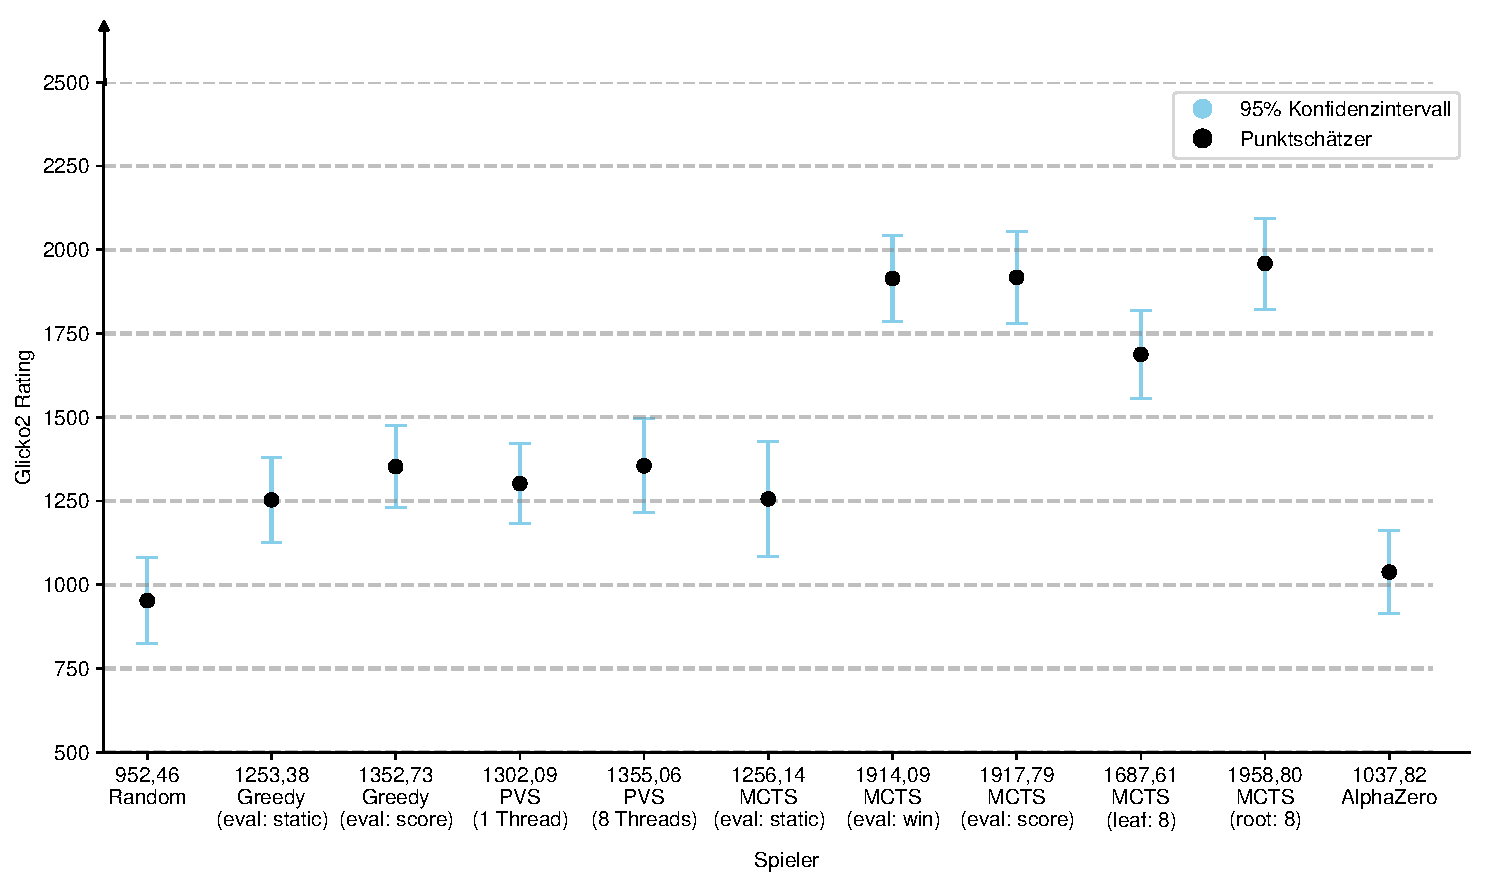
\includegraphics[width=\textwidth]{res/pictures/plots/player-ratings.pdf}
    \caption{Bewertung der Spieler im Glicko-2-Wertungssystem}
    \label{fig:player-ratings}
\end{figure}

In der Rangliste spiegeln sich die Ergebnisse der Vergleichspartien. Auch hier ist der RandomPlayer der schlechteste Spieler. Kurz davor liegt PatchZero. Die Greedy und \ac{PVS} Spieler Varianten teilen sich zusammen in eine ähnliche Bewertungsgruppe ein, wobei der mit Lazy \ac{SMP} parallelisierte \ac{PVS} Spieler die Gruppe anführt. Die \ac{MCTS} Varianten stehen deutlich von den anderen Spielern abgesetzt auf den vorderen Plätzen. Nur der \ac{MCTS} Spieler mit einer statischen Evaluation liegt im Bereich von Greedy- und \ac{PVS}-Spieler. Dies ist nicht verwunderlich, da diese Variante auch eher ähnlich zu diesen Spielern arbeitet, als wie die tatsächlichen \ac{MCTS} Spieler. Die \hyperref[text:leaf-parallelization]{\emph{Leaf Parallelisierung}} bei \ac{MCTS} liegt leicht abgeschlagen von den anderen Varianten, jedoch immer noch weit vor allen anderen Algorithmen, während \hyperref[text:root-parallelization]{\emph{Root Parallelisierung}} einen kleinen Rangvorsprung über die Single-Threaded \ac{MCTS} Varianten aufbauen kann. An dieser Stelle ist es wichtig anzumerken, dass alle in Abbildung \ref{fig:player-ratings} aufgezeigten Glicko-2-Ratings nur relativ zueinander sind und somit nicht mit anderen Glicko-2-Ratings, zum Beispiel von Schach, verglichen werden können.

TODO:

\pagebreak

\section{Ergebnisse gegen die Autoren}

Abschließend wird noch eine \textbf{subjektive} Einschätzung der Spielstärke der einzelnen Computerengines durch die Autoren dieser Arbeit vorgenommen, um die objektivere Einordnung oben zu ergänzen. Dazu wurden verschiedene Spiele gegen die einzelnen Engines gespielt, jedoch nicht genau protokolliert, wie die genauen Ergebnisse aussehen. Die subjektive Einschätzung begrenzt sich dabei jeweils auf die stärkste Variante der unterschiedlichen Computerspielengines.

Gegen den Random Spieler konnten die Autoren einen Großteil der Spiele gewinnen. Generell hat das $7\times 7$ Sonderplättchen für den Random Spieler keinerlei Relevanz, da er immer nur zufällig Flicken über seinen Ablageplan verteilt. So entsteht auf dem Ablageplan der Engine mit sehr hoher Wahrscheinlichkeit eine Zusammenstellung einzelner Fragmente, die untereinander viele Lücken besitzen und keine große gemeinsame Region. Somit erhält der Random Spieler eigentlich nie das $7\times 7$ Sonderplättchen. Für die Autoren dieser Arbeit ist das Sonderplättchen hingegen so gut wie immer erreichbar. Der Punkteunterschied von 7 Punkten, der dadurch am Ende immer existiert, reicht fast immer aus, um das Spiel zu gewinnen. Generell spielt der Random Spieler aber besser als erwartet. Dadurch, dass es in den meisten Fällen deutlich mehr Aktionen gibt, um einen Flicken zu legen (durch alle möglichen Zeilen- und Spaltenpositionen sowie die Rotation und Spiegelung) anstatt die Laufaktion auszuführen, bevorzugt auch der Random Spieler das Legen von Flicken. Somit wird der Ablageplan im Spielverlauf so gut wie möglich gefüllt. Somit erreicht der Random Spieler auch öfters mal Endergebnisse im einstelligen negativen oder positiven Bereich. Solche Ergebnisse lagen auch bei den ersten Spielen der Autoren gegeneinander oft vor.

Die Autoren konnten auch meistens gegen den Greedy Spieler gewinnen. Generell spielt dieser Spieler merklich besser als Random, was sich dadurch auszeichnet, dass die Flickenpositionen auf dem Ablageplan eher wie bei menschlichen Spielern ohne große Lücken sind. Generell wird aber deutlich, dass Greedy dadurch limitiert ist, dass nur eine Position vorausgesehen werden kann. So werden Züge des Gegners nicht beachtet und es findet auch keine längerfristige Planung statt. So schauen sich menschliche Spieler oftmals direkt eine Kombination an Flicken an. Beispielsweise holt ein Spieler sich vielleicht ein schlechteres Teil, um danach direkt noch einmal an der Reihe zu sein und sich ein nun erreichbares besseres Teil zu kaufen.

Der \ac{PVS} Spieler wirkt leicht besser als der Greedy Spieler, was auch mit der Glicko-2 Einschätzung in Abbildung \ref{fig:player-ratings} übereinstimmt. Die Züge wirken teilweise besser überlegt und es werden auch die zuvor angesprochenen Züge mit einer Kombination an Flicken beachtet. Generell können die Autoren aber immer noch gut gegen den \ac{PVS} Spieler gewinnen. Vor allem der Ablageplan des \ac{PVS} Spielers wirkt gegen Ende des Spiels oft noch zu unüberlegt, mit schwierig zu füllenden Lücken. Wahrscheinlich werden durch den StatischenEvaluator die Aktionen bevorzugt, die die restlichen Lücken minimieren. Gleichzeitig ist der \ac{PVS} Spieler dann durch die Ebenen, die vorrausgeschaut werden, begrenzt, sodass die Engine nicht mehr erkennt, dass die restlichen übrigen Flicken nicht mehr dazu geeignet sind, um diese Lücken zu füllen.

Bei dem \ac{MCTS} Spieler hingegen sieht es anders aus. Dieser gewinnt oft gegen die Autoren, ist aber merklich durch seine Bedenkzeit von $10\acs{s}$ beschränkt. Das ist vor allem am Spielanfang bemerkbar. Dort werden oft Flicken fast schon zufällig platziert. Oftmals kann ein Spieler beim ersten Zug alle 1345 möglichen Aktionen ausführen. Der \ac{MCTS} schafft dann $50{.}000-100{.}000$ Iterationen während seiner Bedenkzeit, wobei die wahre Anzahl am Anfang eher bei $50{.}000$ Iterationen liegt. Somit ergibt sich eine durchschnittliche Stichprobengröße von nur 37 möglichen Spielverläufen für jede Aktion. Auch wenn der \ac{MCTS} die Stichproben der Spielverläufe nicht gleichverteilt ausprobiert, sondern häufiger gewinnende Aktionen durch die Tree Policy bevorzugt, wirken die $37$ sehr wenig. Dadurch bildet sich am Anfang ein interessanter häufig zufälliger Ablageplan des \ac{MCTS} Spielers. Im Spielverlauf wird der \ac{MCTS} Spieler dann aber immer besser, da durch den gefüllten Ablageplan weniger Aktionen zur Auswahl stehen und die Simulationsphasen bis zum Spielende kürzer dauern. Somit findet der \ac{MCTS} Spieler auch bei diesem Ablageplan durch die große Anzahl an Iterationen immer genau die Züge, die ihm zum Gewinn führen. Für die Autoren wirkt es so, als sehen sie in der Anfangsphase immer besser dar, trotzdem werden die Spiele dann zum Ende hin immer verloren.

Obwohl der PatchZero Spieler nach der Evaluation leicht besser als Random sein sollte, verhält er sich während des Spielgeschehens für die Autoren genau gleich. Somit gewinnen die Autoren hier auch wieder den Großteil der Spiele. Wahrscheinlich liegt dieses Verhalten daran, dass die Engine nicht genug trainiert worden ist und sich für die Netzwerkevaluation als auf die finale Evaluation eigentlich zufällige Werte ergeben. Dabei ist es nicht erkennbar, ob schon erste kleine Dinge gelernt wurden oder ob sich der PatchZero Spieler tatsächlich zufällig verhält.
\chapter{Fazit}
\label{chapter:fazit}

Im Rahmen der vorliegenden Studienarbeit konnte das Brettspiel Patchwork spieltheoretisch analysiert werden und darauf aufbauend das Spiel als Computerspiel erfolgreich realisiert werden. Das Brettspiel besitzt sehr viele mögliche Spielzüge und Spielzustände, wodurch eine optimale beziehungsweise sehr schnelle Implementierung der Computergegner im Computerspiel schwer zu erreichen ist. Fast alle Computerspielengines funktionieren entsprechend der Erwartungen an dieselben, allerdings existieren einige Einschränkungen. Der \ac{PVS} Spieler schneidet deutlich schlechter ab als der \ac{MCTS} Spieler und dieser Vorsprung ist durch die Verbesserungen, welche an der Spielengine gemacht werden können, schwer aufzuholen da bei der \ac{MCTS} Spielengine im gleichen Maße noch Optimierungen stattfinden können. Die Ausnahmen macht der PatchZero Spieler, da er die Erwartungen verfehlt. Bei der Spielengine fehlt vermutlich noch weiteres und längeres Training des neuronalen Netzes, um durch kontinuierliche Evaluation bei besseren Trainingsständen den Spieler besser einzuschätzen. In der Zukunft könnten weitere Computergegner-Typen, Variationen oder Verbesserungen der bestehenden Computergegner umgesetzt werden und auf Tauglichkeit für das Computerspiel getestet werden. Außerdem sollten für eine bessere Evaluation aller Computerspielengines die Anzahl der Spiele untereinander signifikant erhöht werden, um eine statistische Sicherheit bei der Bewertung der Spieler zu erhalten.

Das Ziel der Umsetzung des Computerspiels als interaktives System mit intuitiver Benutzeroberfläche wurde nicht erreicht. Zwar wurde das Brettspiel auf ein digitales Medium übertragen und das Spiel lässt sich als einzelner Spieler spielen, allerdings ist zum jetzigen Zeitpunkt nur eine Interaktion mit der \ac{CLI} Schnittstelle möglich, da die Benutzeroberfläche noch nicht finalisiert wurde. Dementsprechend kann nicht bewertet werden, inwieweit die nahtlose Transformation des Brettspiels zum Computerspiel gelungen ist.

Als weiteren Ausblick für die Zukunft der Studienarbeit könnte die grundlegende Umsetzung von Patchwork als Computerspiel weiterreichend nach Optimierungsmöglichkeiten gesucht werden, um durch Optimierung die Performance des Computerspiels zu verbessern. Außerdem könnte das neu erschlossene digitalen Medium des Computerspiels dazu verwendet werden, die Unabhängigkeit der Entfernung auszunutzen, um das ehemalige Brettspiel in ein kompetitives Online-Mehrspieler-Spiel umzuwandeln.

% ---- Literaturverzeichnis
\cleardoublepage
\renewcommand*{\chapterpagestyle}{plain}
\pagestyle{plain}
\pagenumbering{Roman}                   % Römische Seitenzahlen
\setcounter{page}{\numexpr\value{savepage}+1}
\printbibliography[title=Literaturverzeichnis]

% ---- Anhang
\appendix
\clearpage
\pagenumbering{Roman}  % römische Seitenzahlen für Anhang
\chapter{Anhangskapitel}
\label{anhang:chapter-anhangskapitel}

TODO:

Tabelle/Text mit Patchwork Terminologie

\pagebreak

\chapter{Patchwork}

% \section{Patchwork \textemdash Terminologie}

% TODO:

\section{Zeitpläne}

\begin{figure}[!ht]
    \centering
    \begin{minipage}{.48\textwidth}
        \centering
        \begin{tikzpicture}
            \node [inner sep=0pt,,outer sep=0pt,clip,rounded corners=0.15cm] (image) at (0,0) {\includegraphics[width=0.75\linewidth]{res/pictures/assets/time-board-side-1.png}};
            \drawshadow{image}
        \end{tikzpicture}
    \end{minipage}
    \hfill
    \begin{minipage}{.48\textwidth}
        \centering
        \begin{tikzpicture}
            \node [inner sep=0pt,,outer sep=0pt,clip,rounded corners=0.15cm] (image) at (0,0) {\includegraphics[width=0.75\linewidth]{res/pictures/assets/time-board-side-2.png}};
            \drawshadow{image}
        \end{tikzpicture}
    \end{minipage}
    \vspace*{-0.05cm}
    \caption{Die zwei Seiten des Zeitplans}
    \label{fig:patchwork-time-board}
\end{figure}

\section{Ablagepläne}

\begin{figure}[!ht]
    \centering
    \begin{minipage}{.48\textwidth}
        \centering
        \begin{tikzpicture}
            \node [inner sep=0pt,,outer sep=0pt,clip,rounded corners=0.15cm] (image) at (0,0) {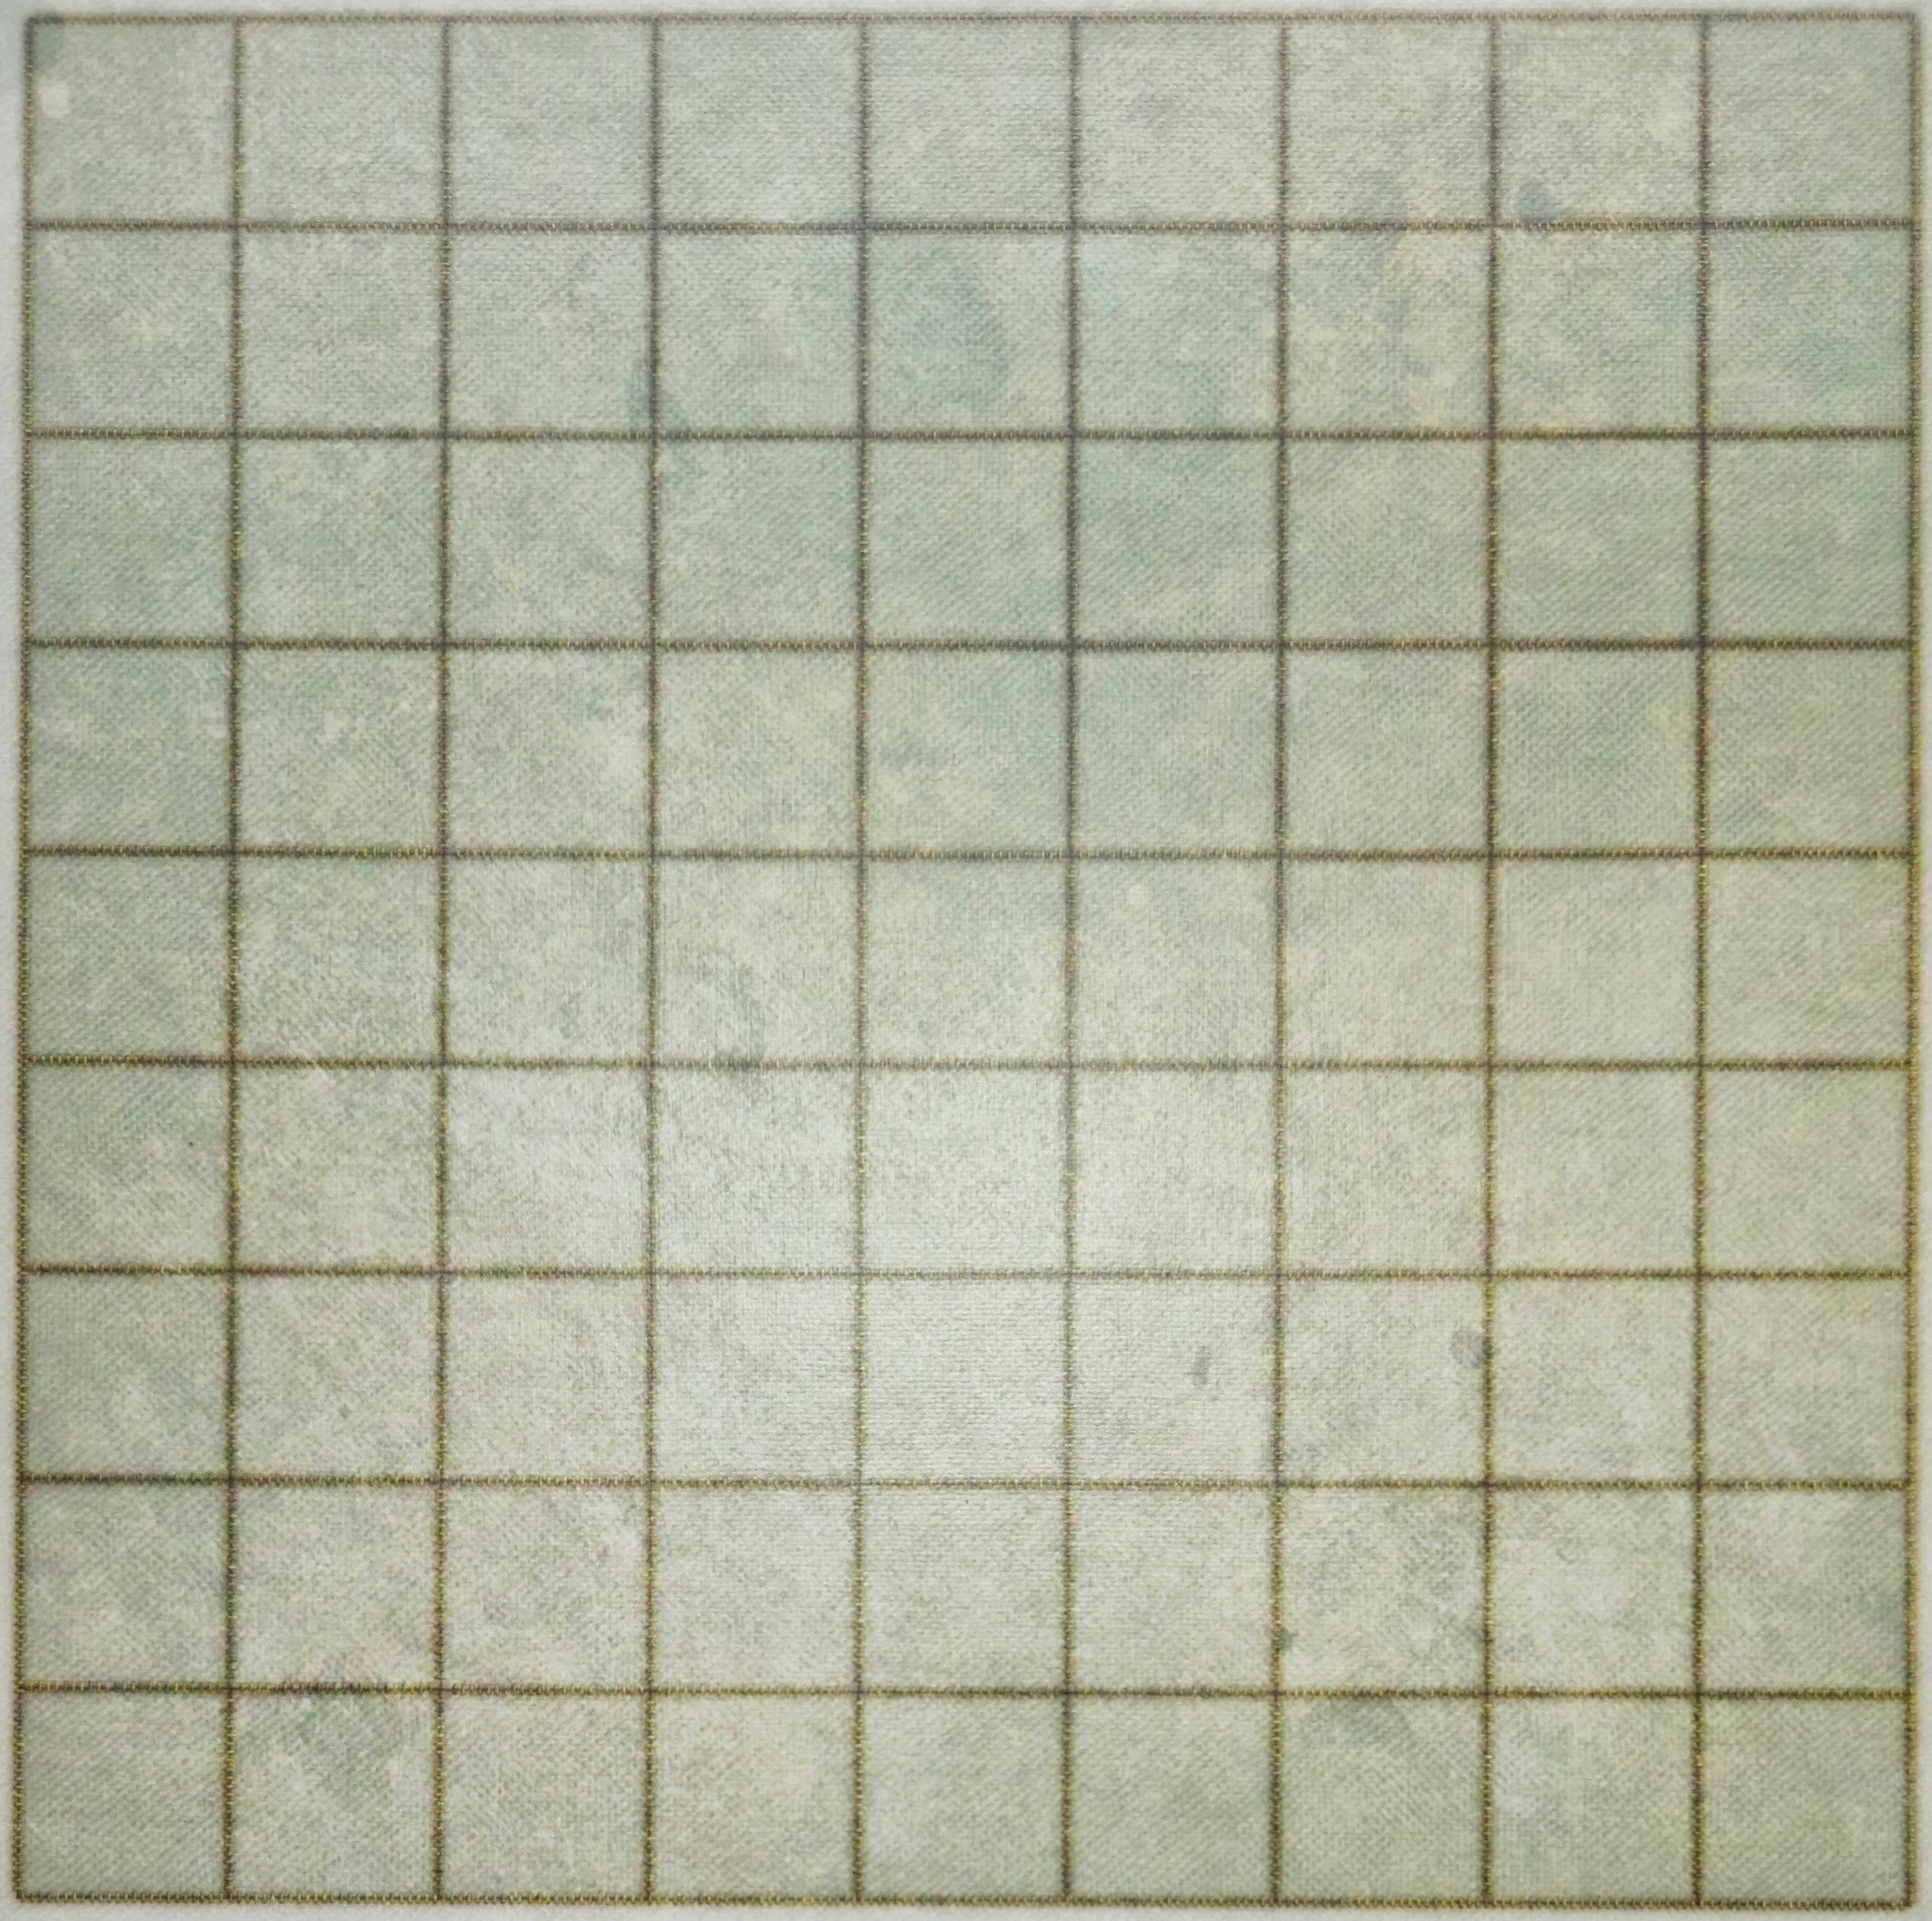
\includegraphics[width=0.75\linewidth]{res/pictures/assets/board-player-1.png}};
            \drawshadow{image}
        \end{tikzpicture}
    \end{minipage}
    \hfill
    \begin{minipage}{.48\textwidth}
        \centering
        \begin{tikzpicture}
            \node [inner sep=0pt,,outer sep=0pt,clip,rounded corners=0.15cm] (image) at (0,0) {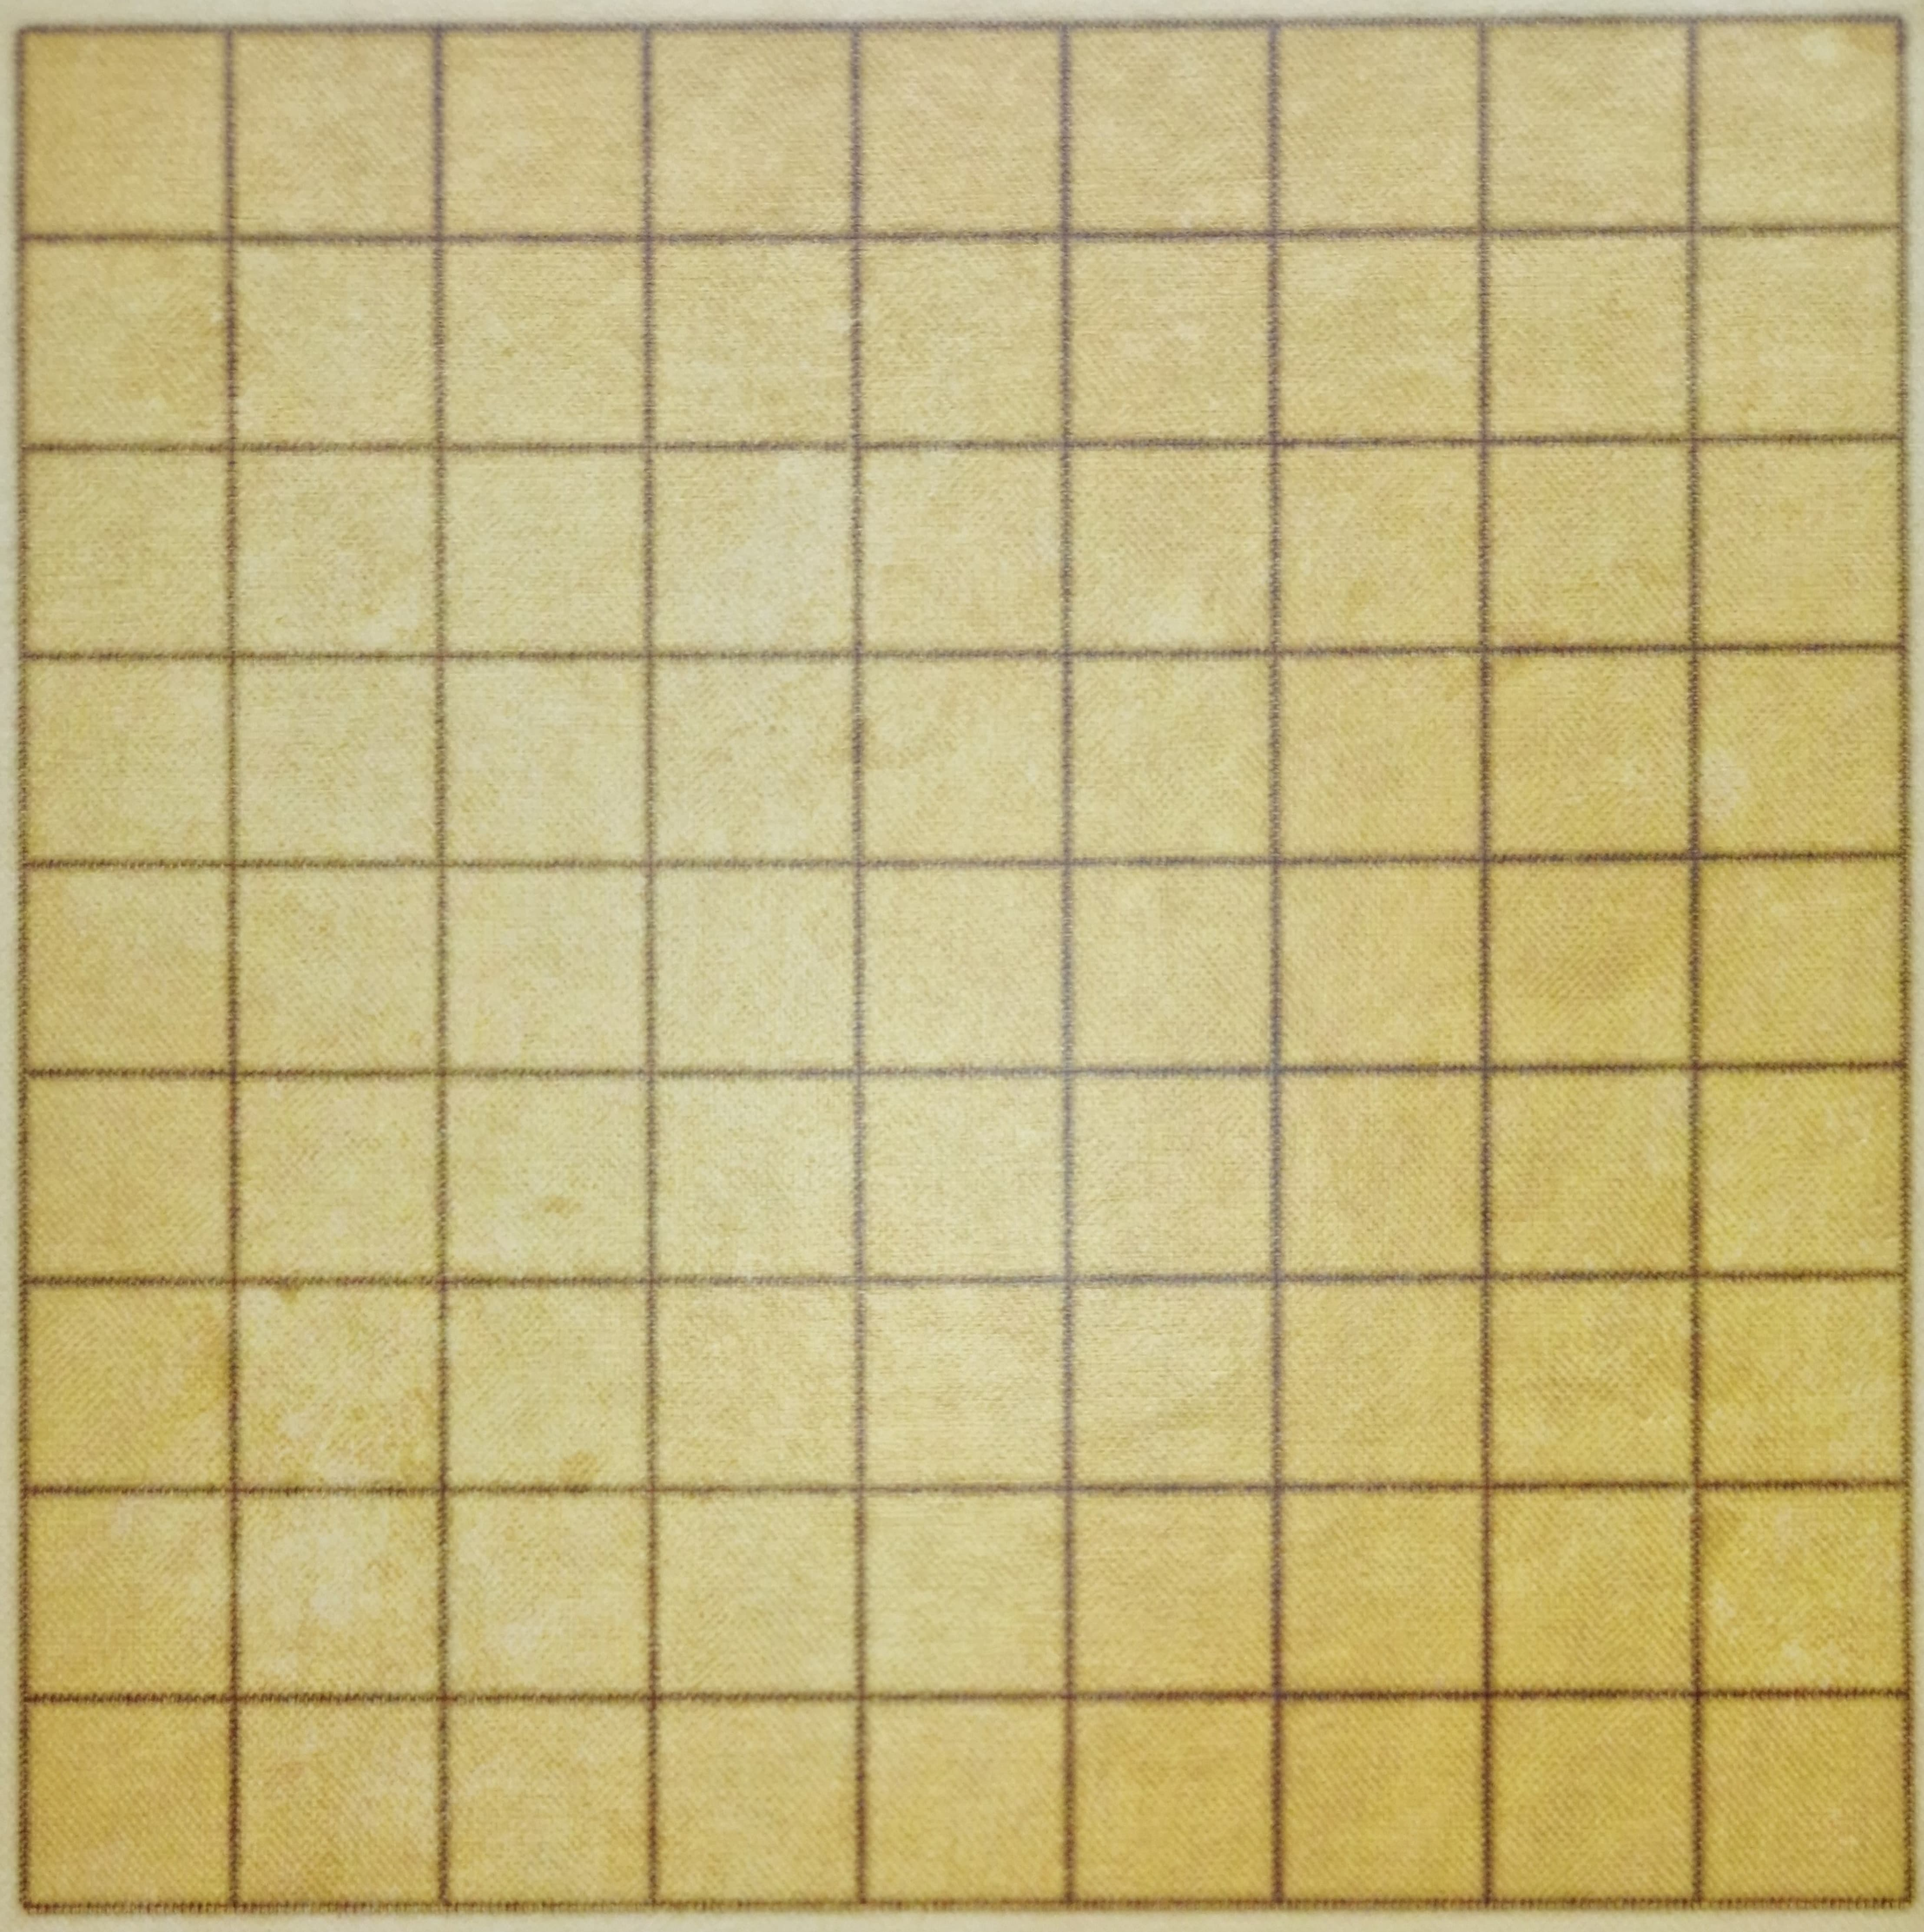
\includegraphics[width=0.75\linewidth]{res/pictures/assets/board-player-2.png}};
            \drawshadow{image}
        \end{tikzpicture}
    \end{minipage}
    \vspace*{-0.05cm}
    \caption{Ablagepläne (Decken) der Spieler}
    \label{fig:patchwork-player-quilt-board}
\end{figure}

\pagebreak

\section{Flicken}
\label{anhang:section-patchwork-patches}

% \setlength{\tabcolsep}{5pt}

\begin{longtable}[t]{|c|c|c|c|c|c|c|}
    \hline
    \raisebox{0pt}[3ex][2ex]{Flicken}                                                                                                                 & ID   & Felder & \makecell{ Knopf                                              \\ Kosten } & \makecell{ Zeit \\ Kosten } & \makecell{ Knopf \\ Einkommen } & $\frac{\text{Knopfeinkommen}}{\text{Felder}\, \cdot\, \text{Zeitkosten}}$ \\ \hline
    \endfirsthead
    \multicolumn{7}{c}{\tablename\ \thetable\ -- \textit{Fortsetzung von der vorherigen Seite}}                                                                                                                                       \\
    \hline
    \raisebox{0pt}[3ex][2ex]{Flicken}                                                                                                                 & ID   & Felder & \makecell{ Knopf                                              \\ Kosten } & \makecell{ Zeit \\ Kosten } & \makecell{ Knopf \\ Einkommen } & $\frac{\text{Knopfeinkommen}}{\text{Felder}\, \cdot\, \text{Zeitkosten}}$ \\ \hline
    \endhead
    \hline \multicolumn{7}{r}{\textit{Fortsetzung auf der nächsten Seite}}                                                                                                                                                            \\
    \endfoot
    \hline
    \caption{Alle 33 Flicken in Patchwork}
    \label{tabelle:patchwork-patches}
    \endlastfoot
    \adjustbox{valign=m, max width=0.2\textwidth, max height=0.1\textheight}{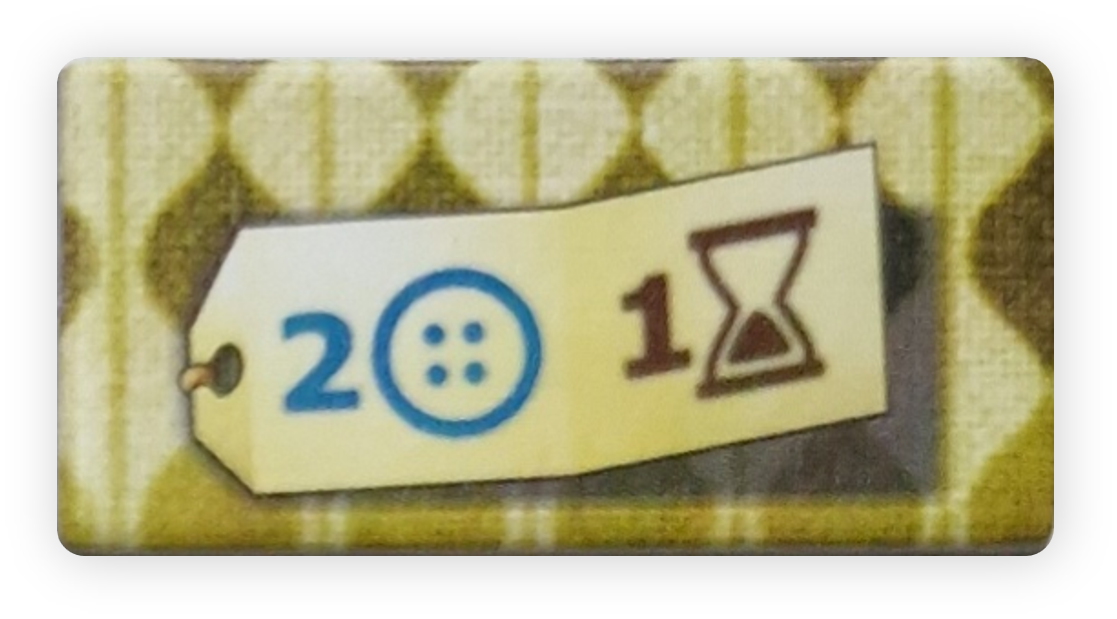
\includegraphics[width=0.2\textwidth]{res/pictures/assets/00-front.png}} & $0$  & $2$    & $2$              & $1$ & $0$ & $0$                            \\ \hline
    \adjustbox{valign=m, max width=0.2\textwidth, max height=0.1\textheight}{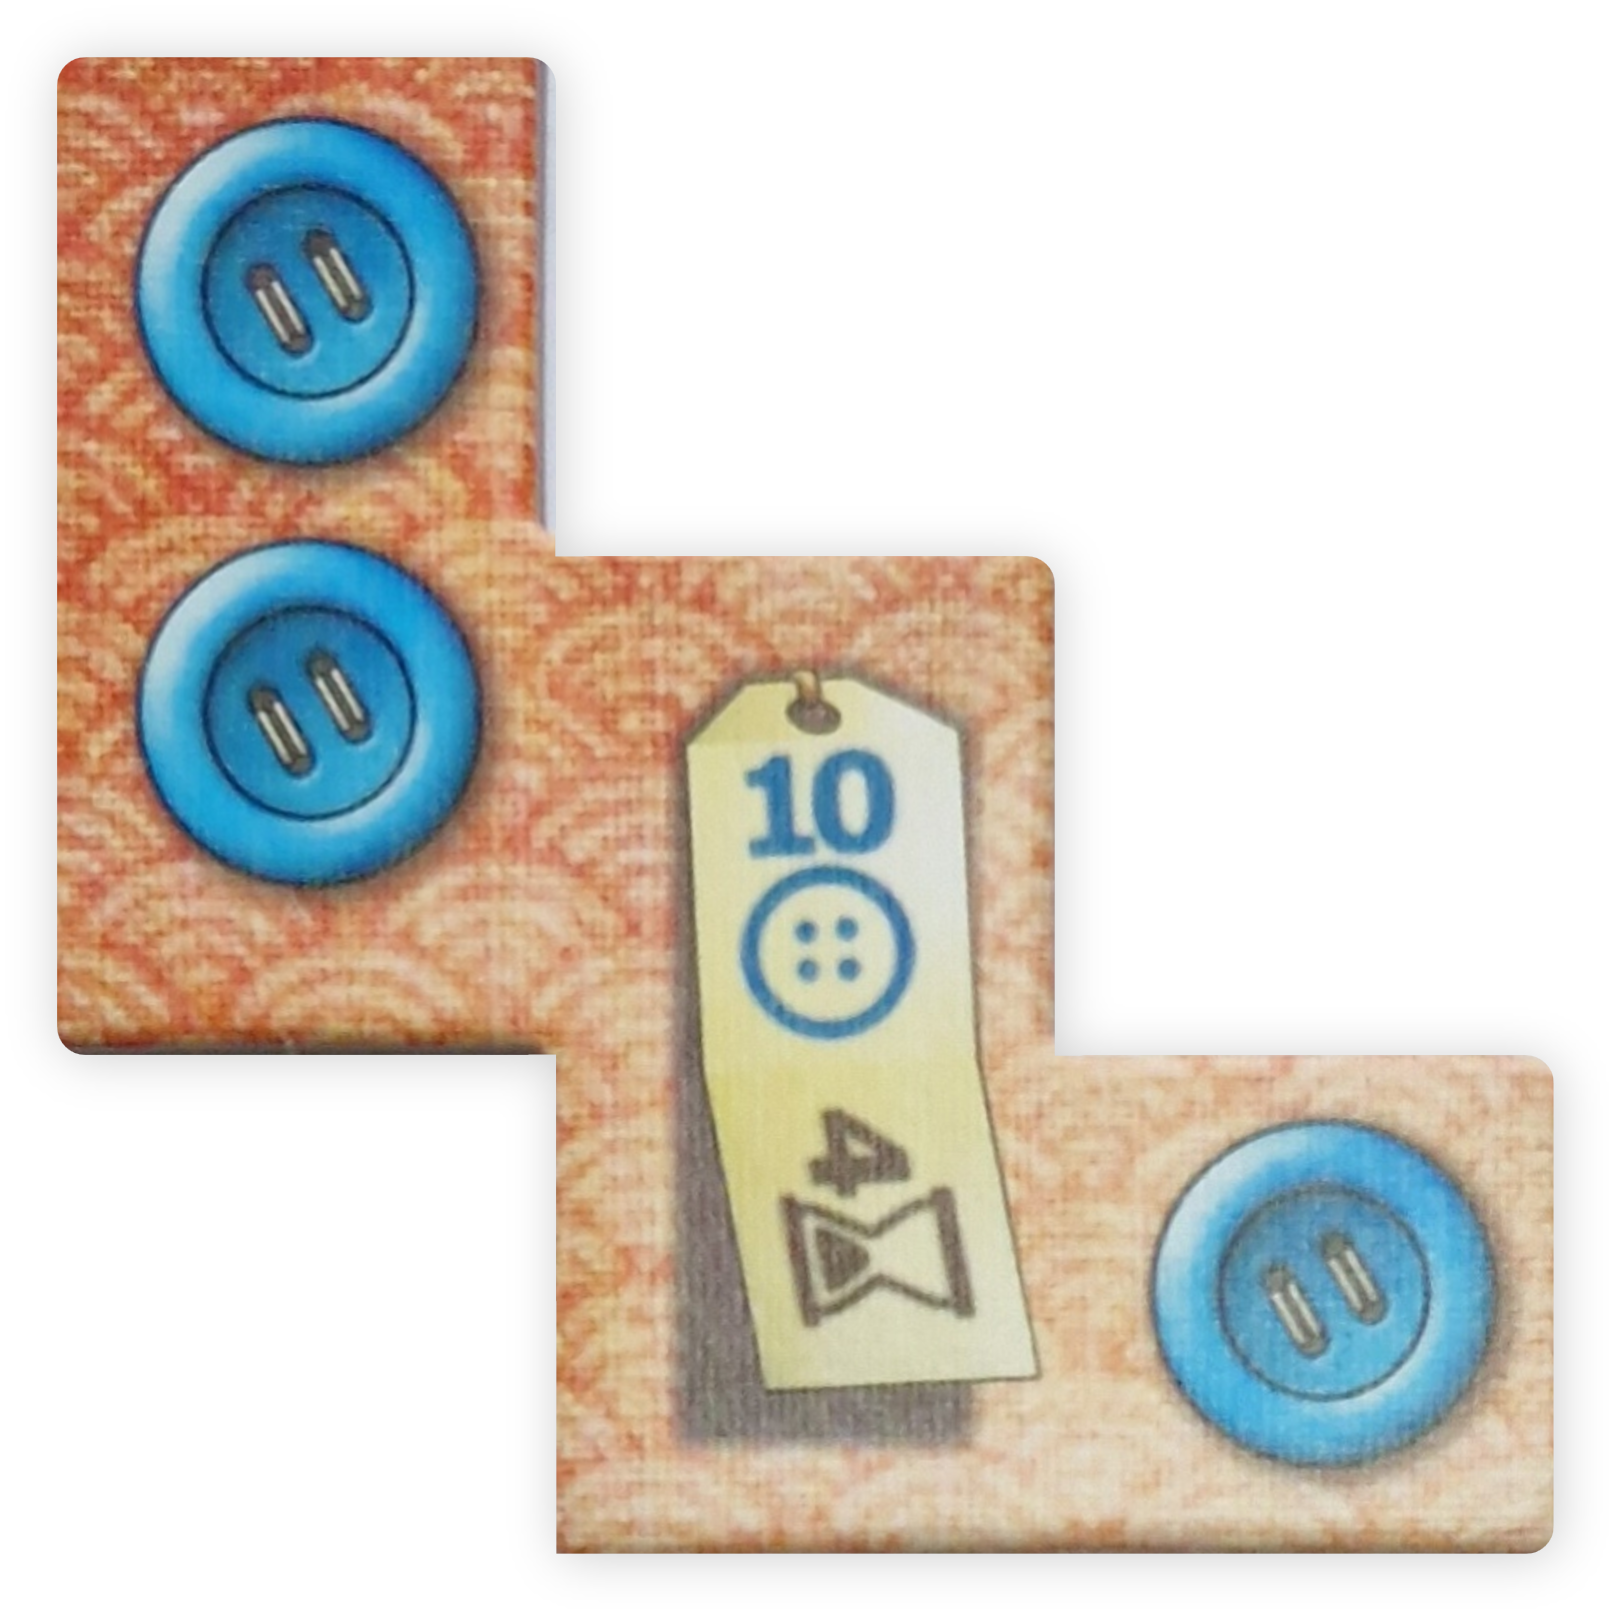
\includegraphics[width=0.2\textwidth]{res/pictures/assets/01-front.png}} & $1$  & $5$    & $10$             & $4$ & $3$ & $\frac{3}{20} = 0{,}15$        \\ \hline
    \adjustbox{valign=m, max width=0.2\textwidth, max height=0.1\textheight}{\includegraphics[width=0.2\textwidth]{res/pictures/assets/02-front.png}} & $2$  & $8$    & $5$              & $3$ & $1$ & $\frac{1}{24} \approx 0{,}042$ \\ \hline
    \adjustbox{valign=m, max width=0.2\textwidth, max height=0.1\textheight}{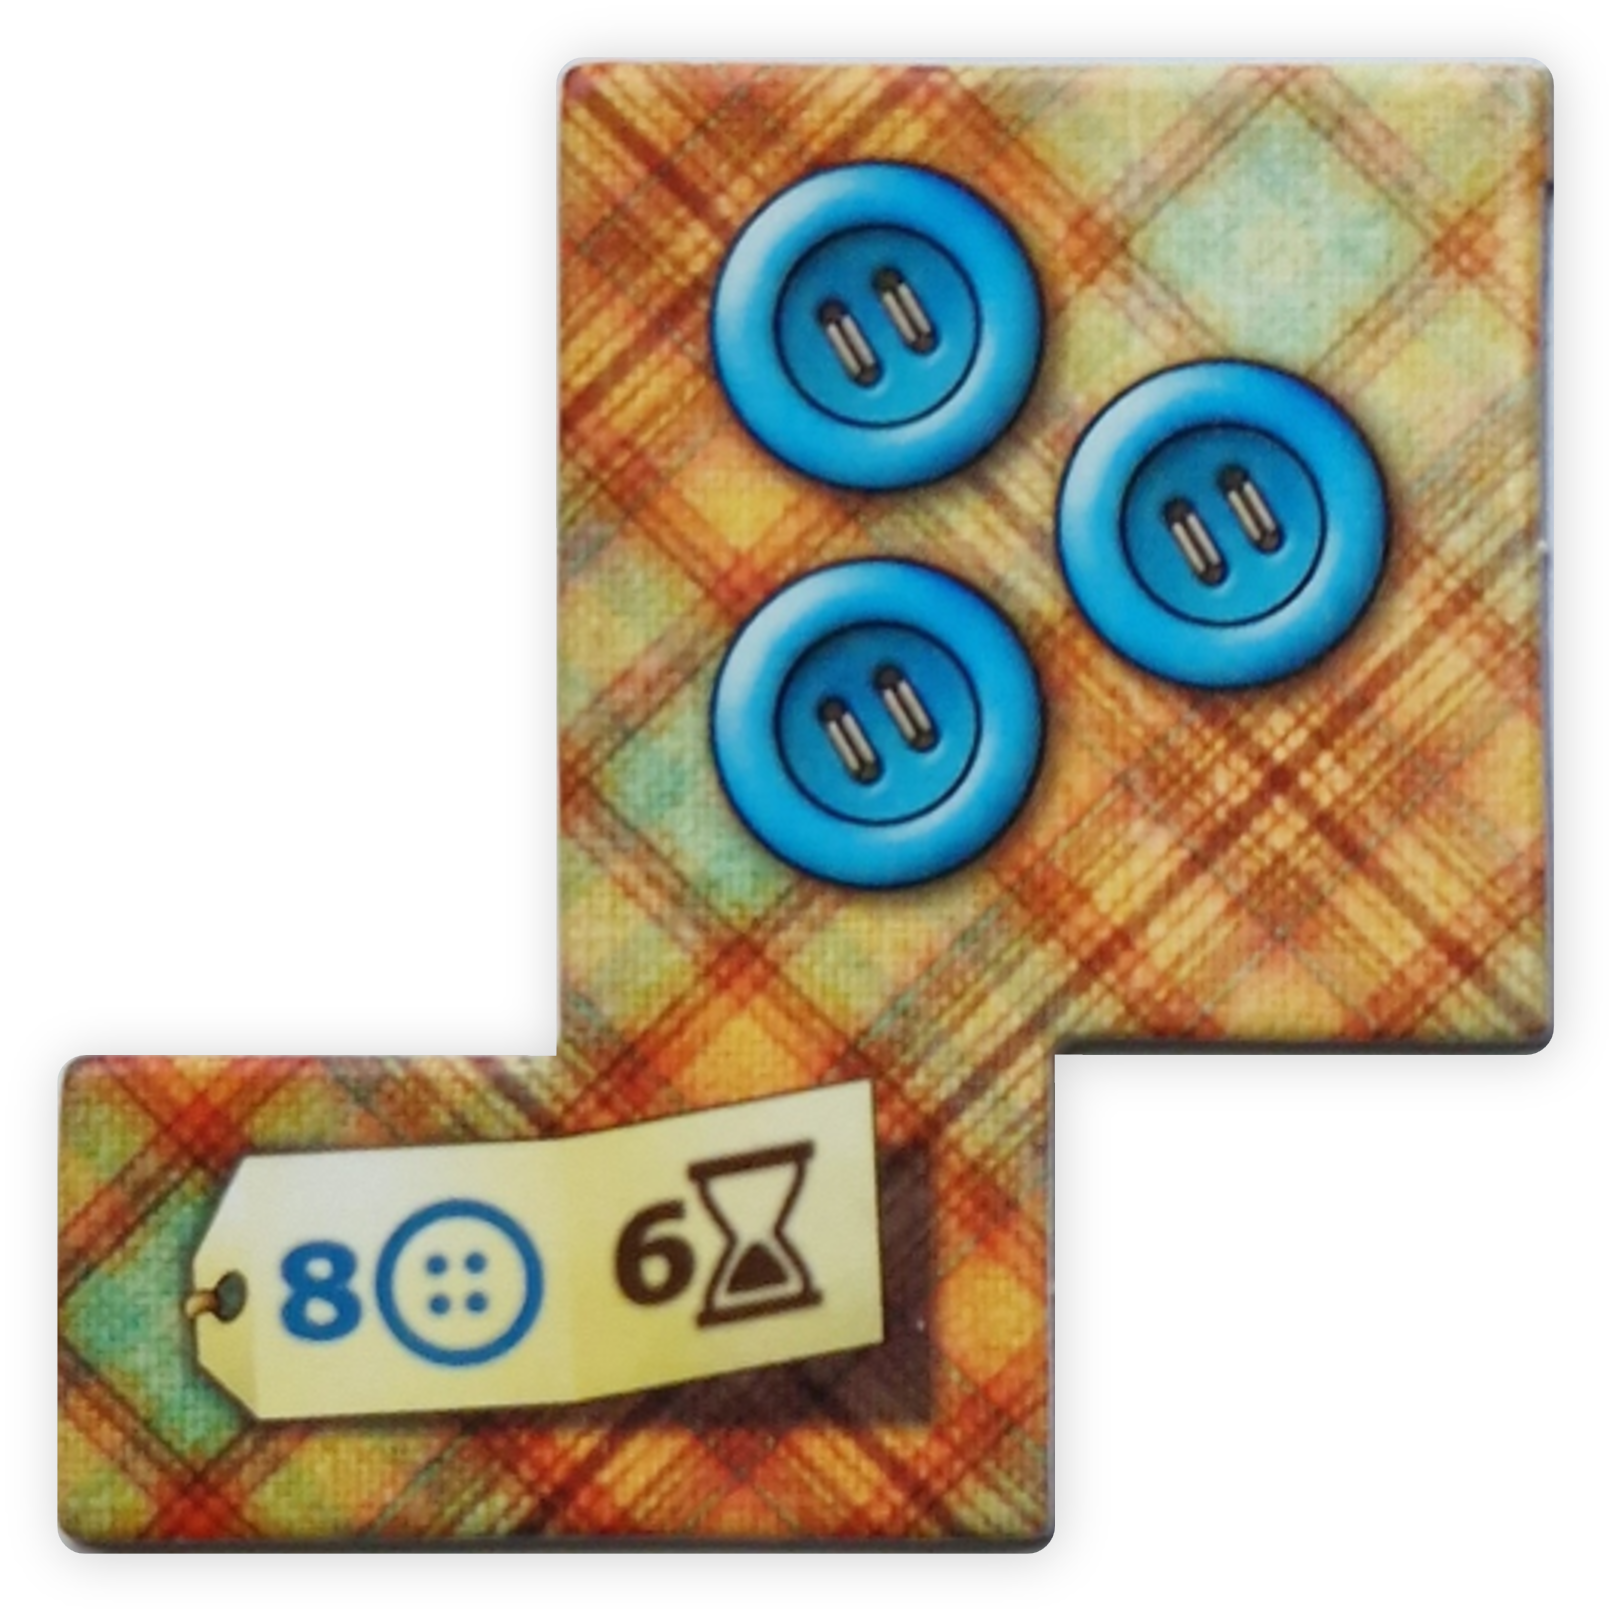
\includegraphics[width=0.2\textwidth]{res/pictures/assets/03-front.png}} & $3$  & $6$    & $8$              & $6$ & $3$ & $\frac{1}{12} \approx 0{,}083$ \\ \hline
    \adjustbox{valign=m, max width=0.2\textwidth, max height=0.1\textheight}{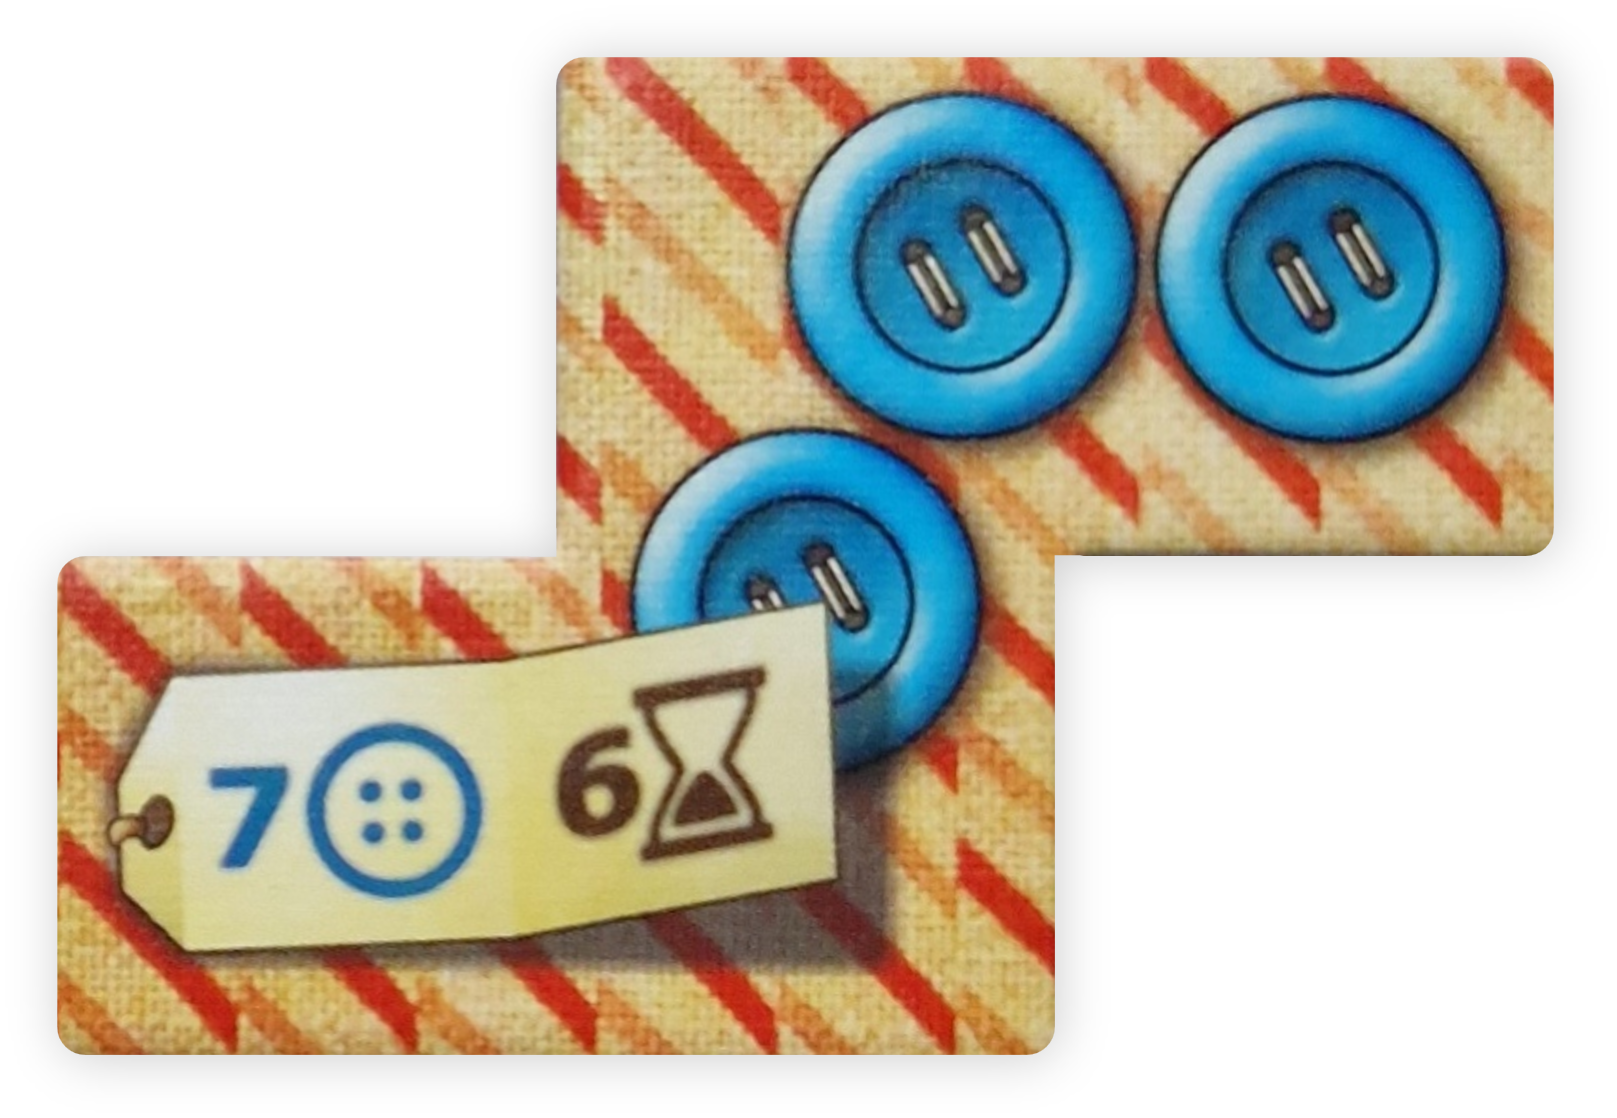
\includegraphics[width=0.2\textwidth]{res/pictures/assets/04-front.png}} & $4$  & $4$    & $7$              & $6$ & $3$ & $\frac{1}{8} = 0{,}125$        \\ \hline
    \adjustbox{valign=m, max width=0.2\textwidth, max height=0.1\textheight}{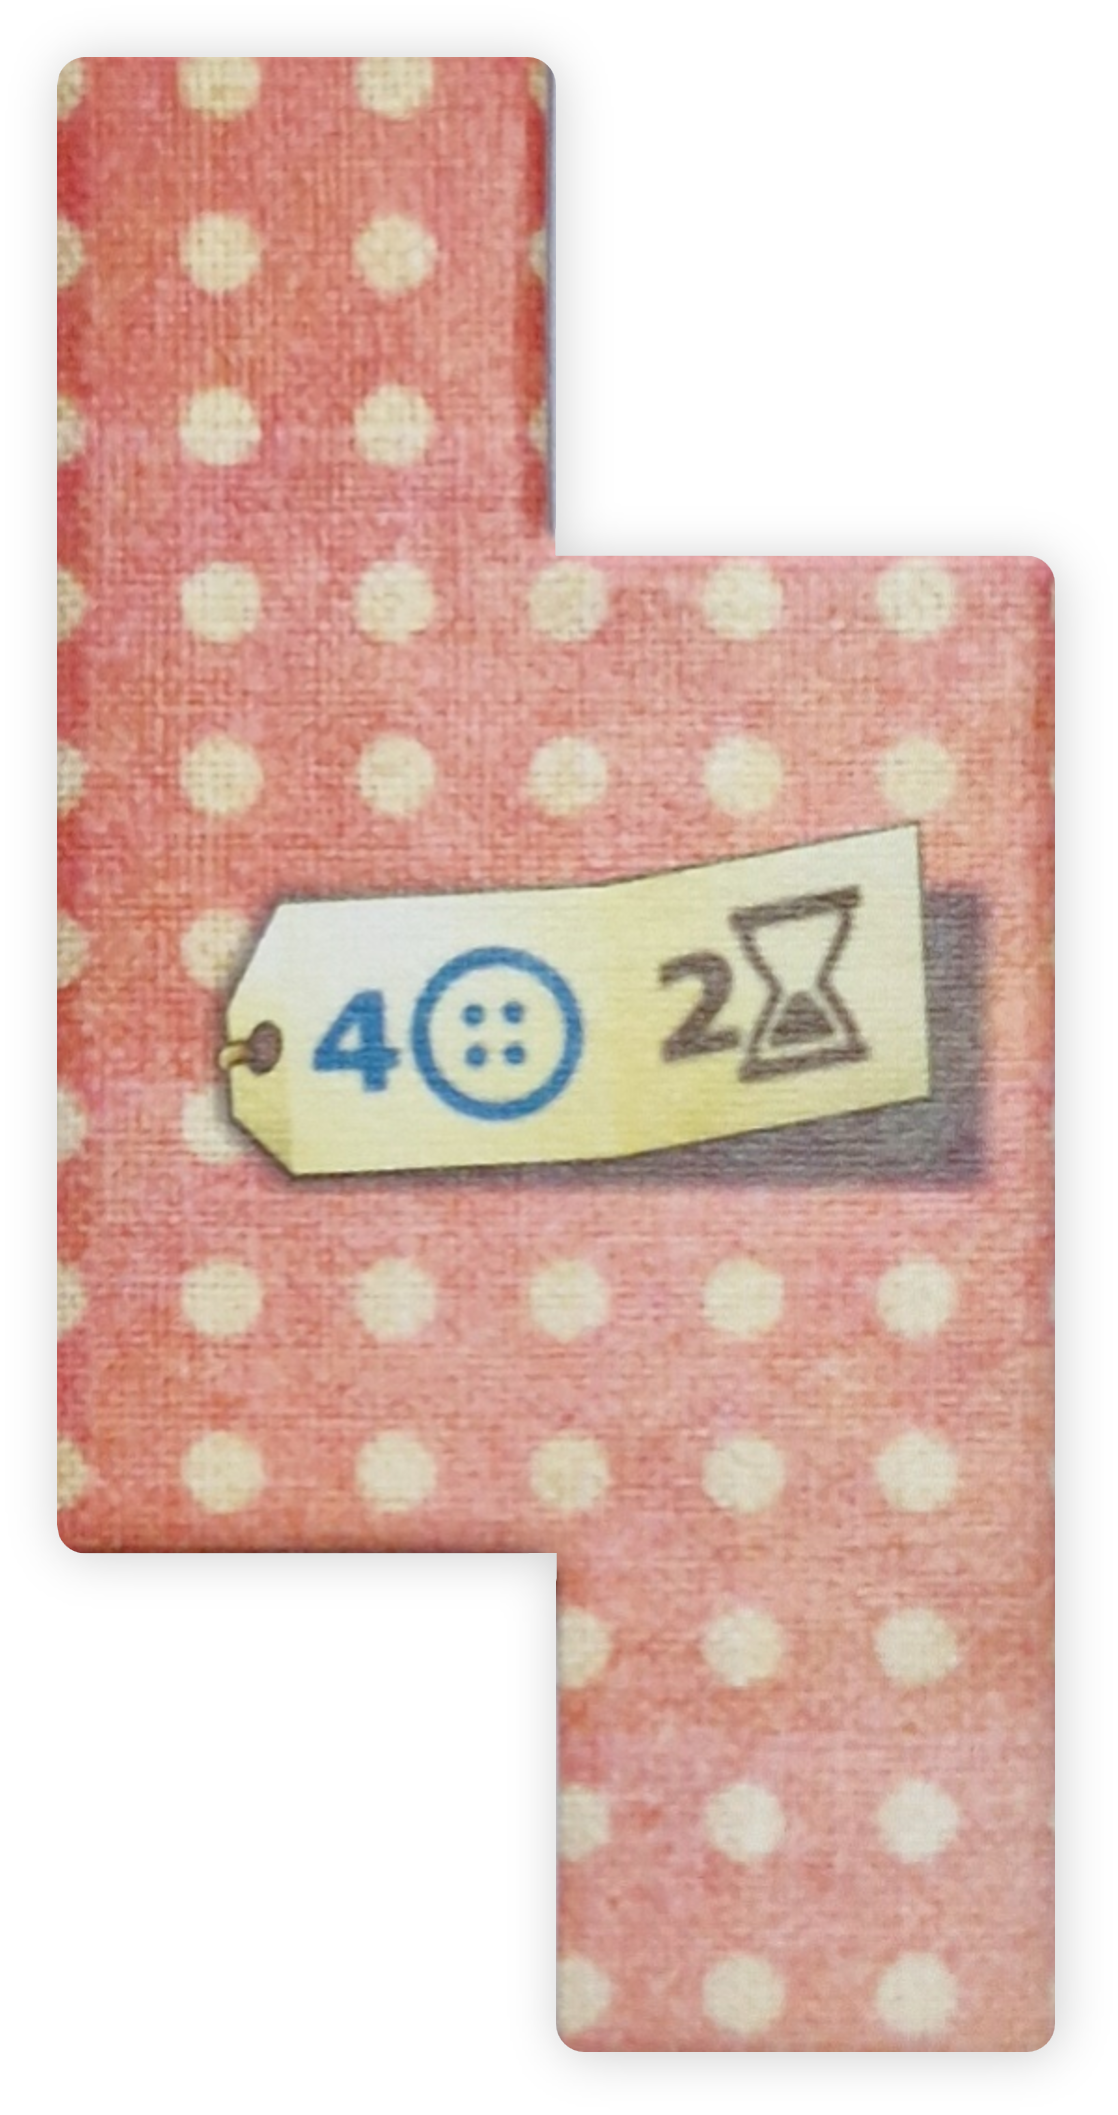
\includegraphics[width=0.2\textwidth]{res/pictures/assets/05-front.png}} & $5$  & $6$    & $4$              & $2$ & $0$ & $0$                            \\ \hline
    \adjustbox{valign=m, max width=0.2\textwidth, max height=0.1\textheight}{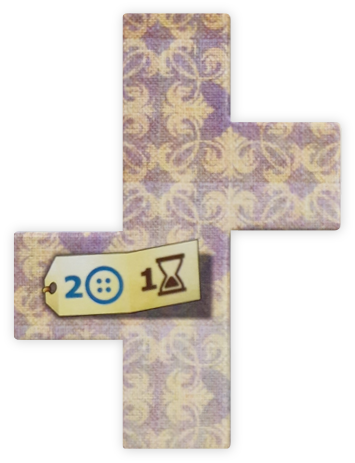
\includegraphics[width=0.2\textwidth]{res/pictures/assets/06-front.png}} & $6$  & $6$    & $2$              & $1$ & $0$ & $0$                            \\ \hline
    \adjustbox{valign=m, max width=0.2\textwidth, max height=0.1\textheight}{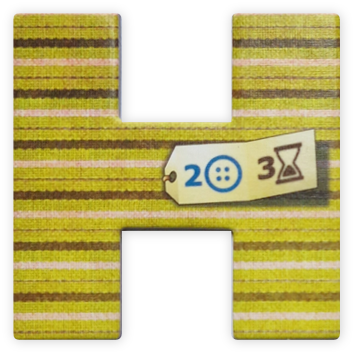
\includegraphics[width=0.2\textwidth]{res/pictures/assets/07-front.png}} & $7$  & $7$    & $2$              & $3$ & $0$ & $0$                            \\ \hline
    \adjustbox{valign=m, max width=0.2\textwidth, max height=0.1\textheight}{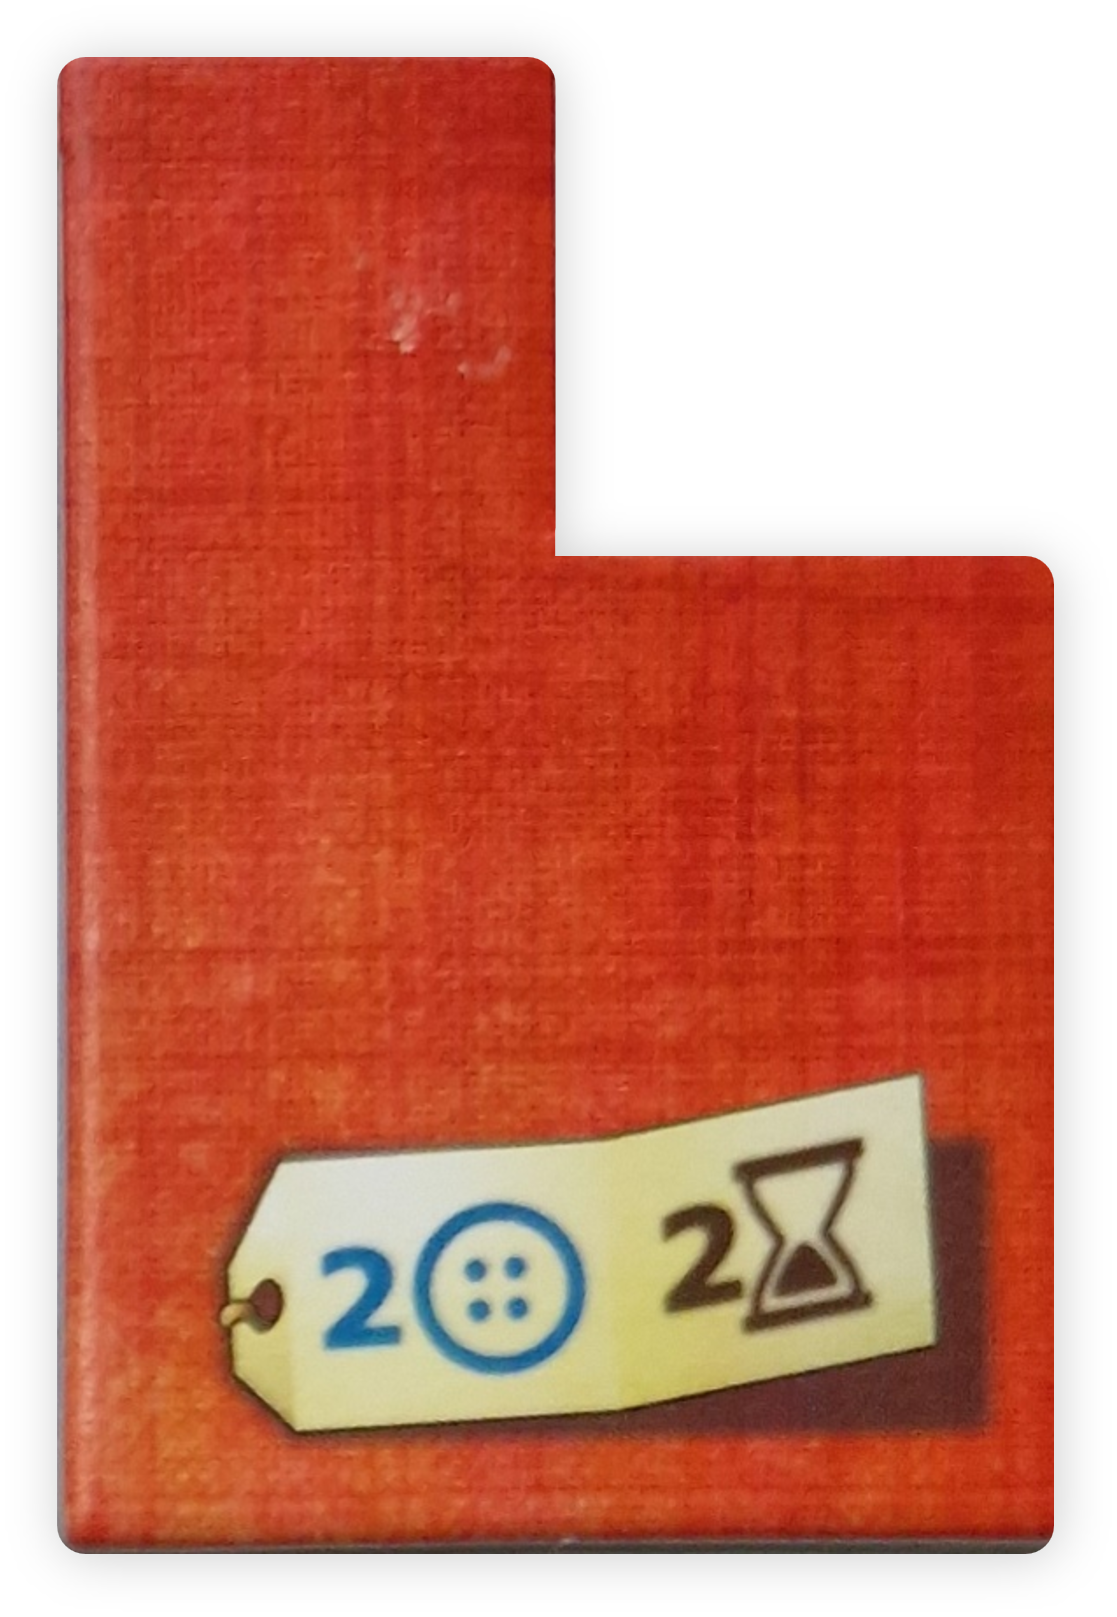
\includegraphics[width=0.2\textwidth]{res/pictures/assets/08-front.png}} & $8$  & $5$    & $2$              & $2$ & $0$ & $0$                            \\ \hline
    \adjustbox{valign=m, max width=0.2\textwidth, max height=0.1\textheight}{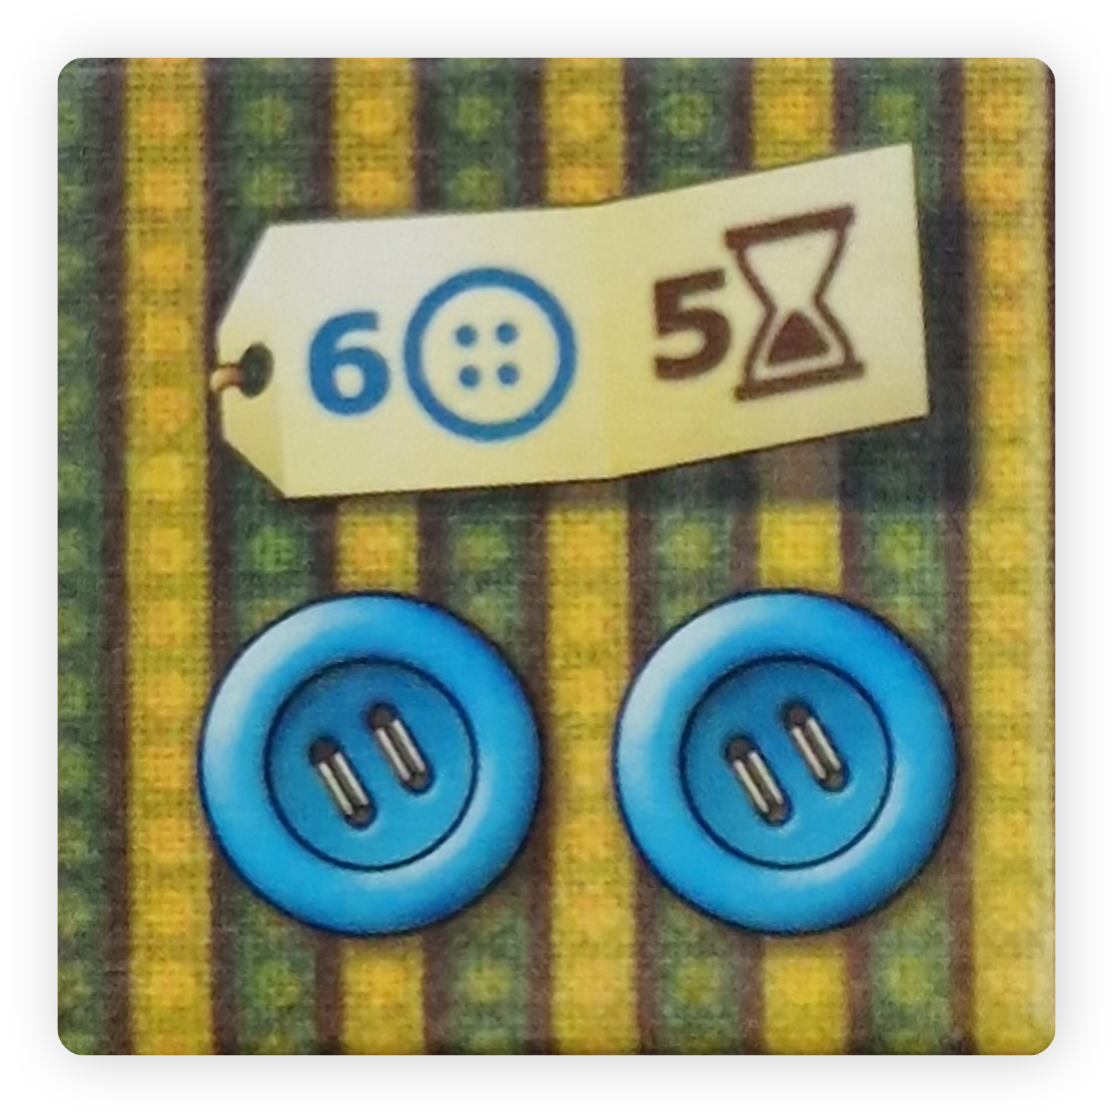
\includegraphics[width=0.2\textwidth]{res/pictures/assets/09-front.png}} & $9$  & $4$    & $6$              & $5$ & $2$ & $\frac{1}{10} = 0{,}1$         \\ \hline
    \adjustbox{valign=m, max width=0.2\textwidth, max height=0.1\textheight}{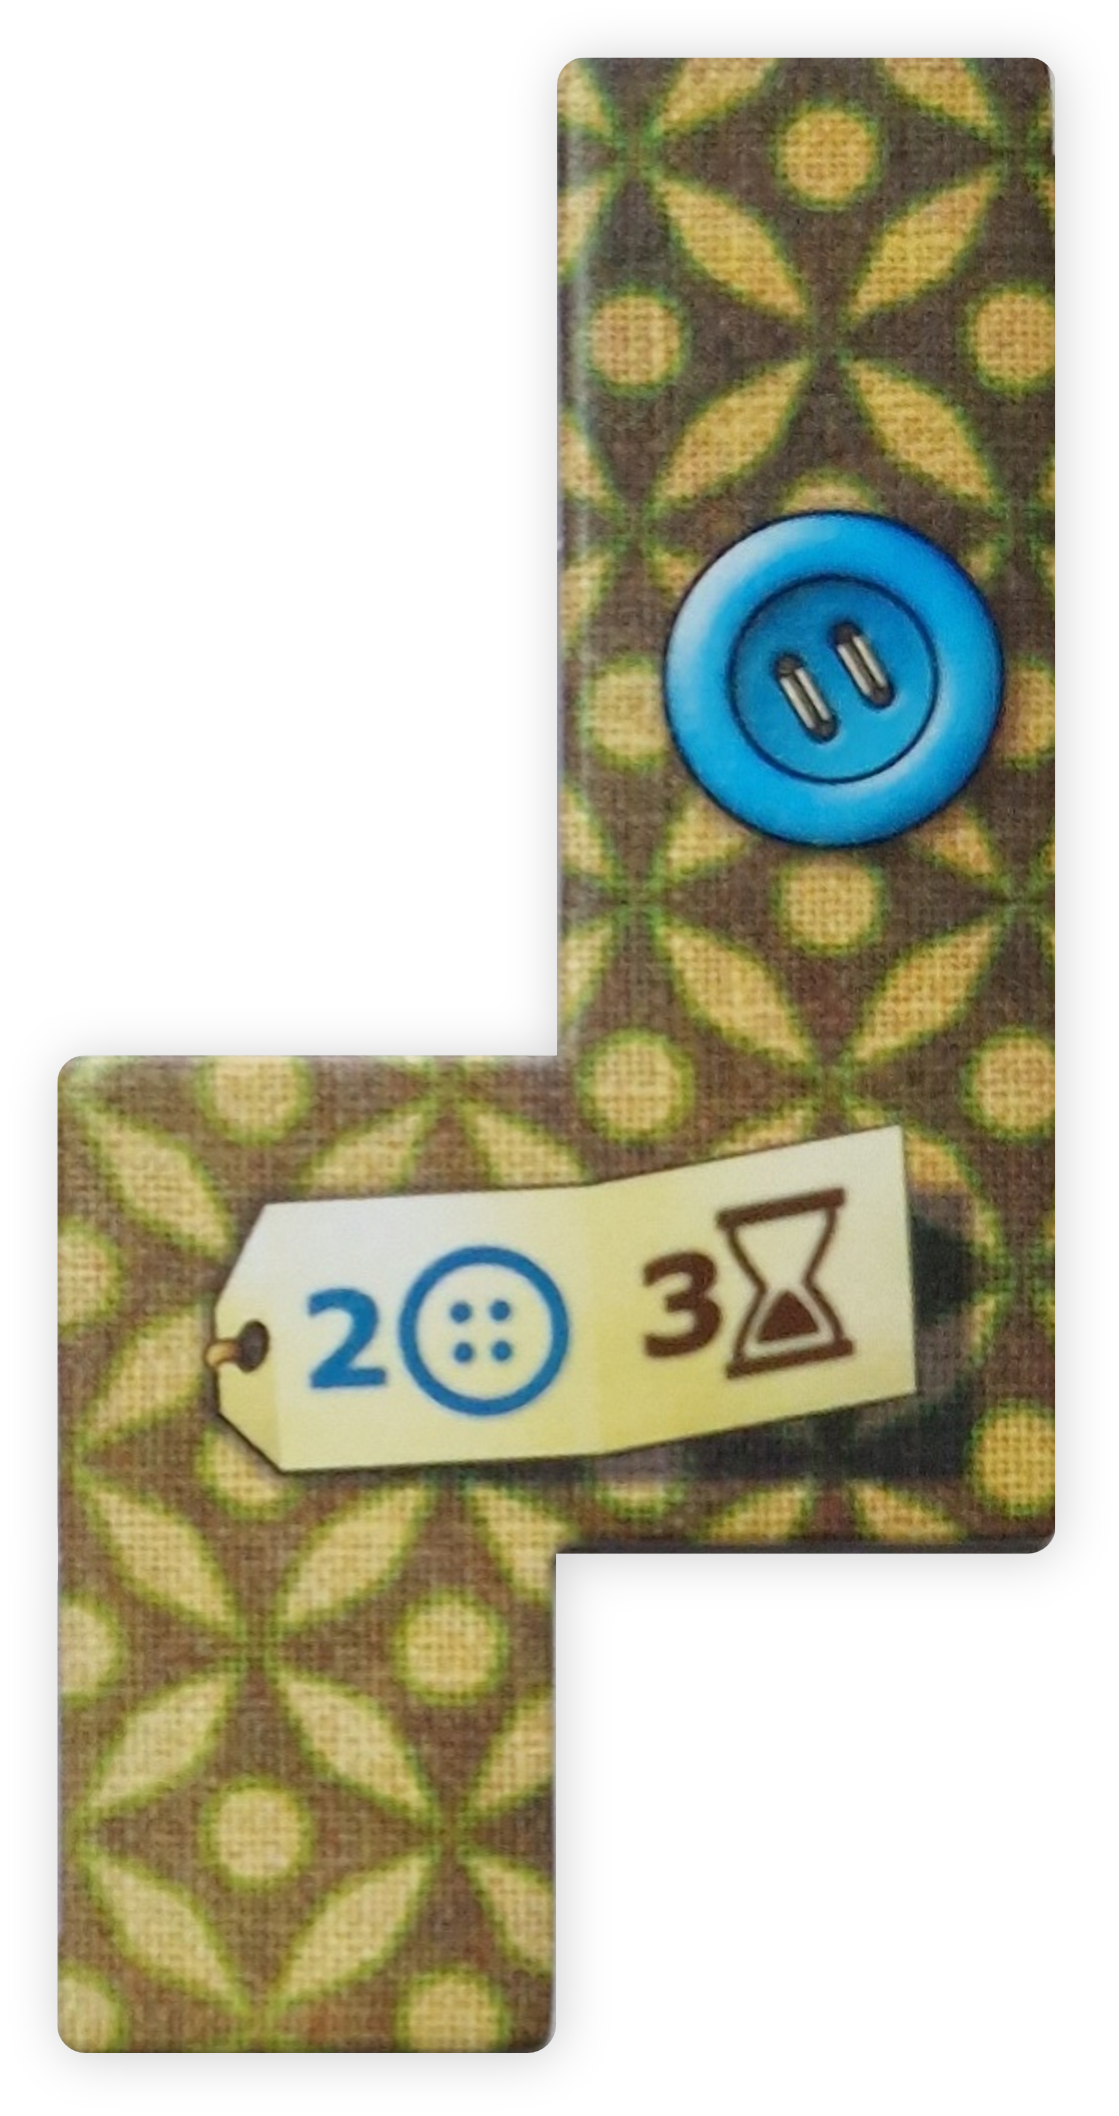
\includegraphics[width=0.2\textwidth]{res/pictures/assets/10-front.png}} & $10$ & $5$    & $2$              & $3$ & $1$ & $\frac{1}{15} \approx 0{,}067$ \\ \hline
    \adjustbox{valign=m, max width=0.2\textwidth, max height=0.1\textheight}{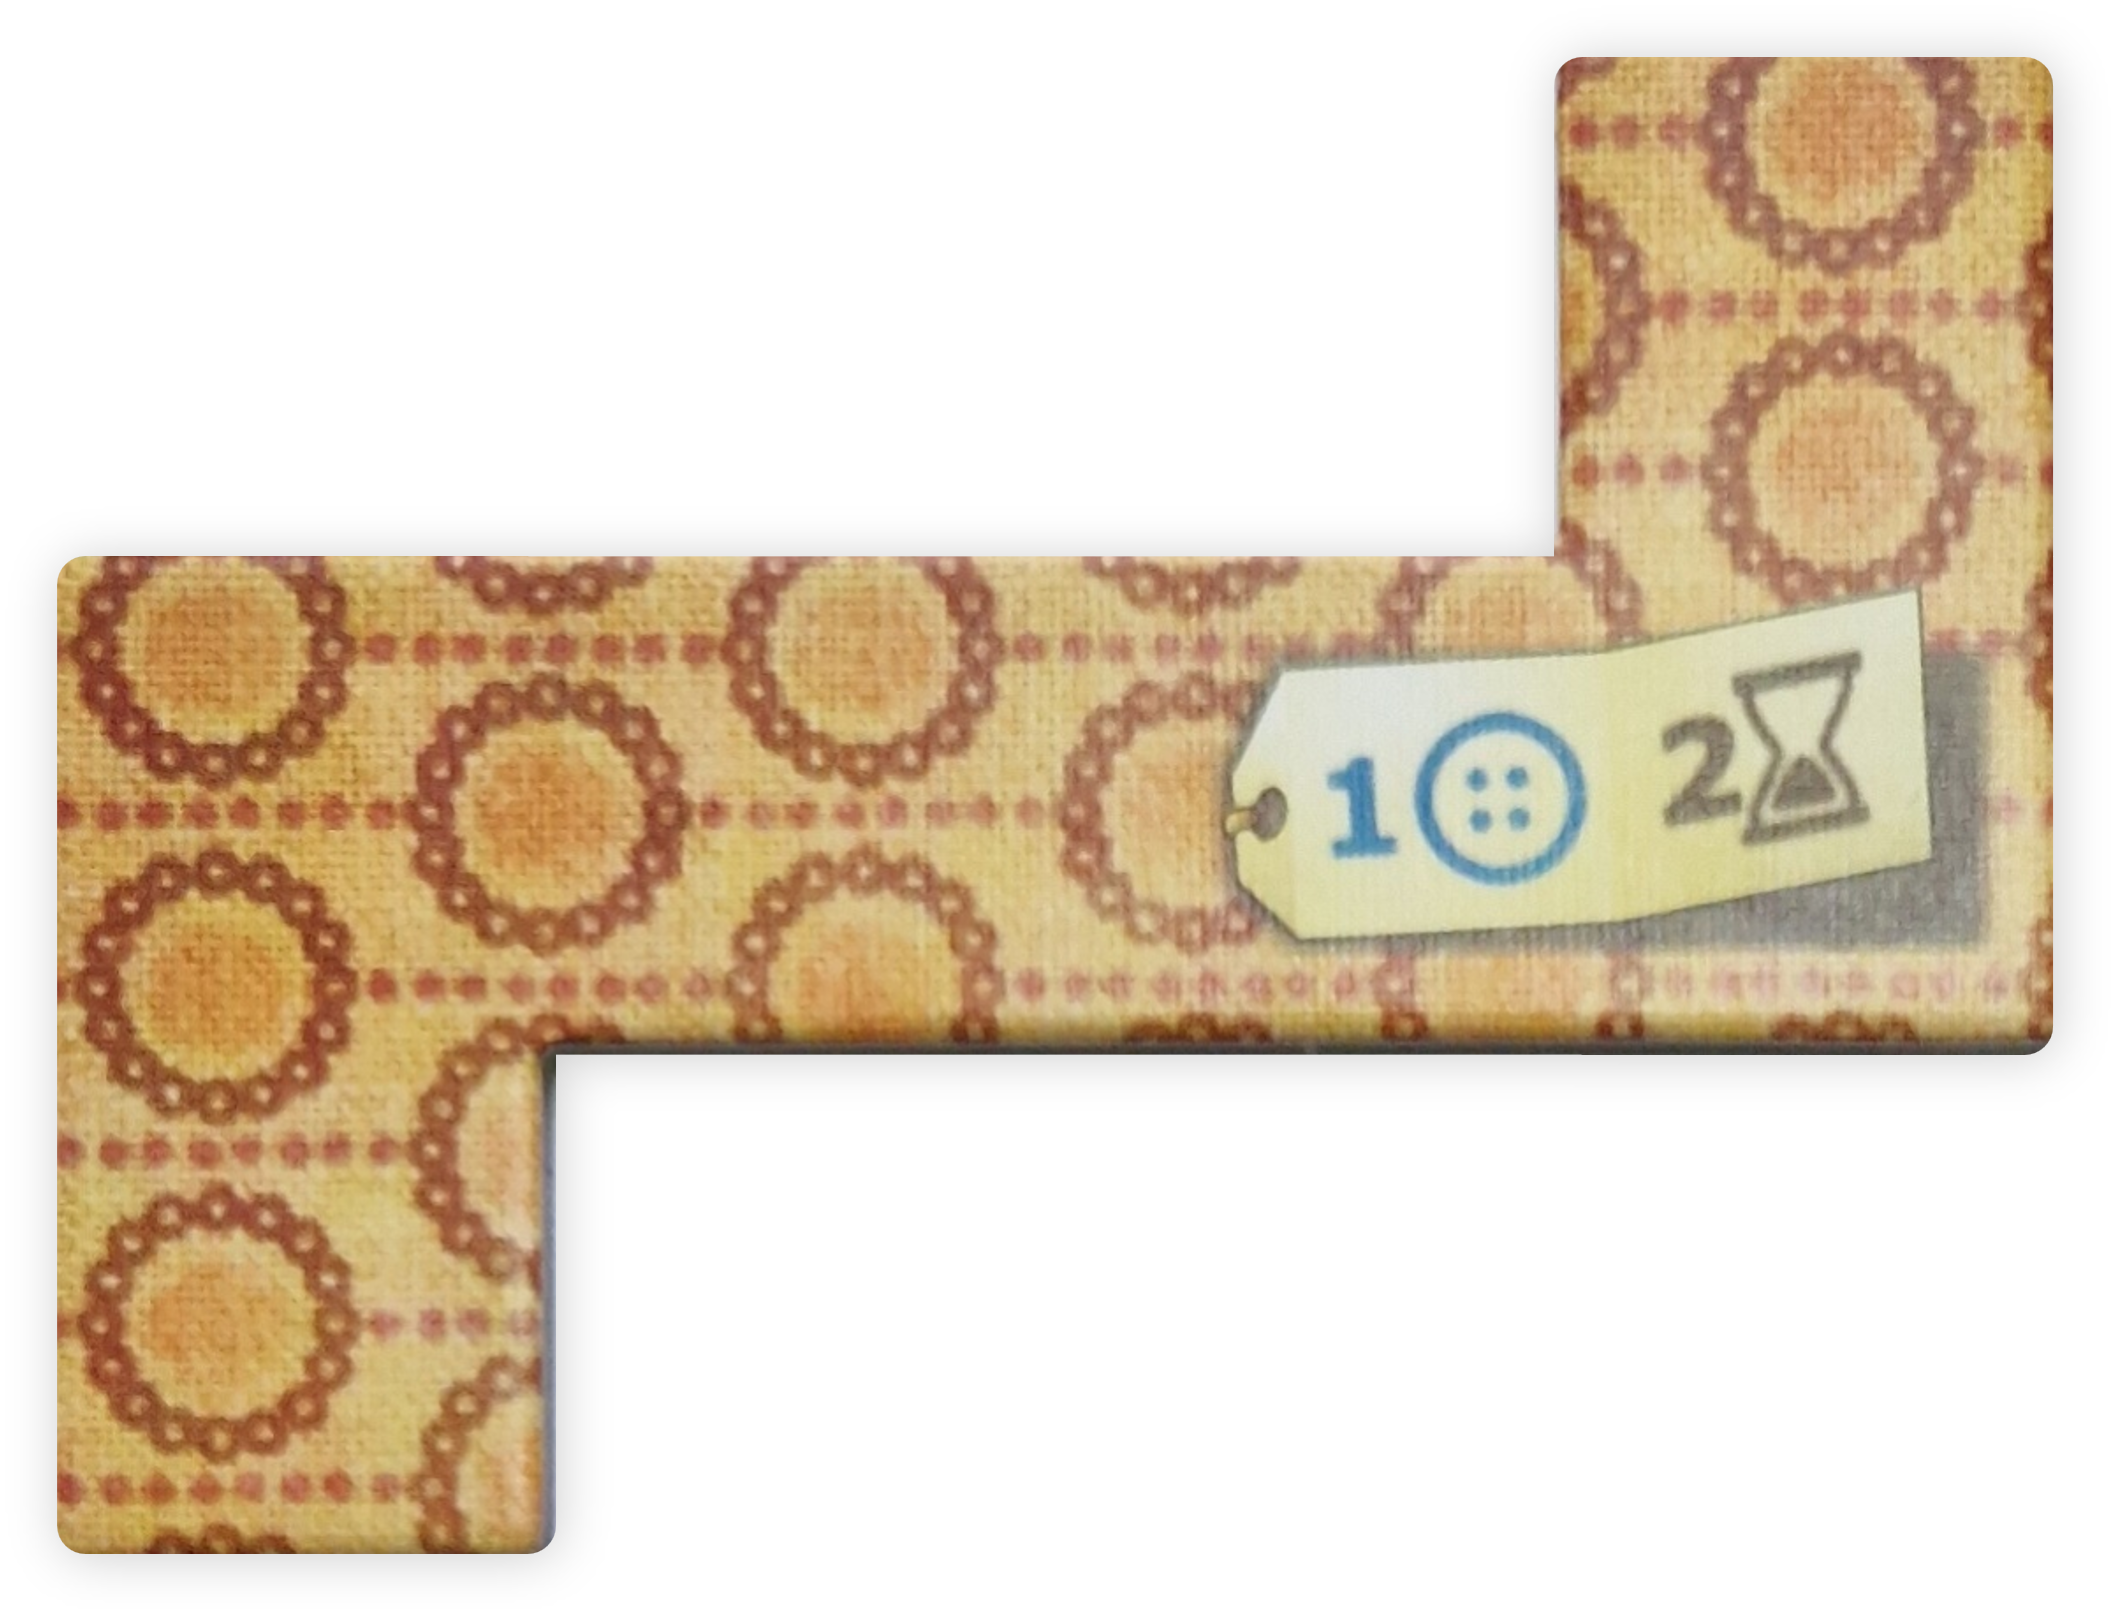
\includegraphics[width=0.2\textwidth]{res/pictures/assets/11-front.png}} & $11$ & $6$    & $1$              & $2$ & $0$ & $0$                            \\ \hline
    \adjustbox{valign=m, max width=0.2\textwidth, max height=0.1\textheight}{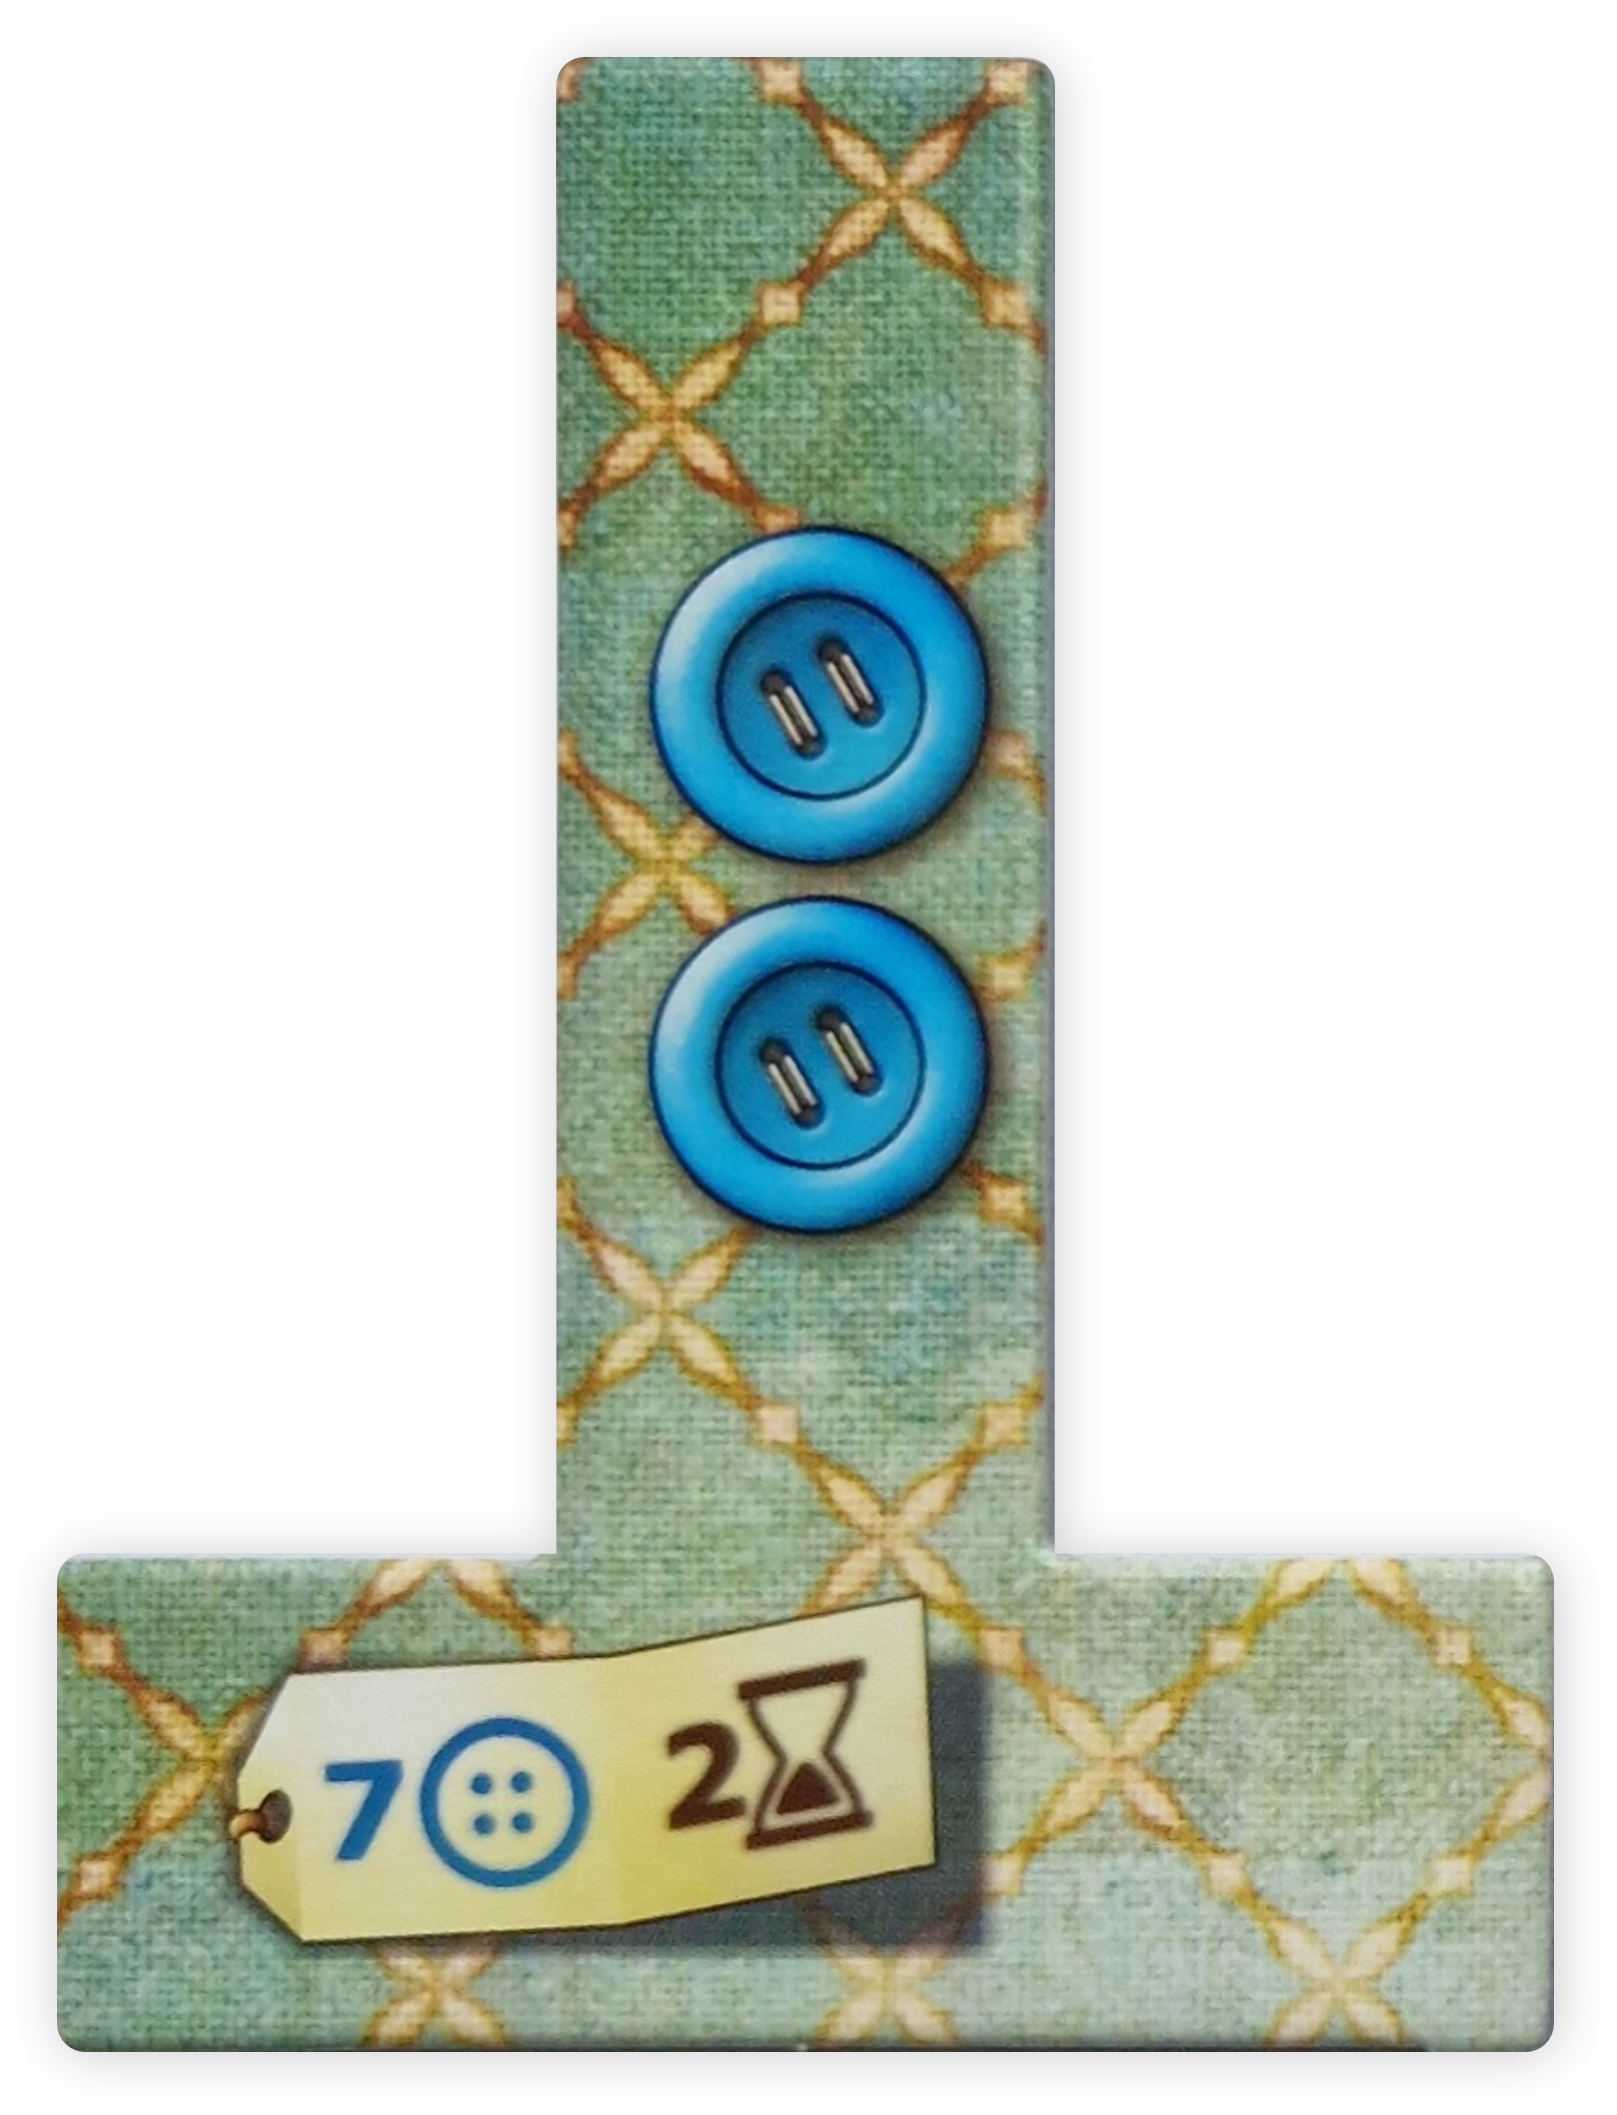
\includegraphics[width=0.2\textwidth]{res/pictures/assets/12-front.png}} & $12$ & $6$    & $10$             & $5$ & $3$ & $\frac{1}{10} = 0{,}1$         \\ \hline
    \adjustbox{valign=m, max width=0.2\textwidth, max height=0.1\textheight}{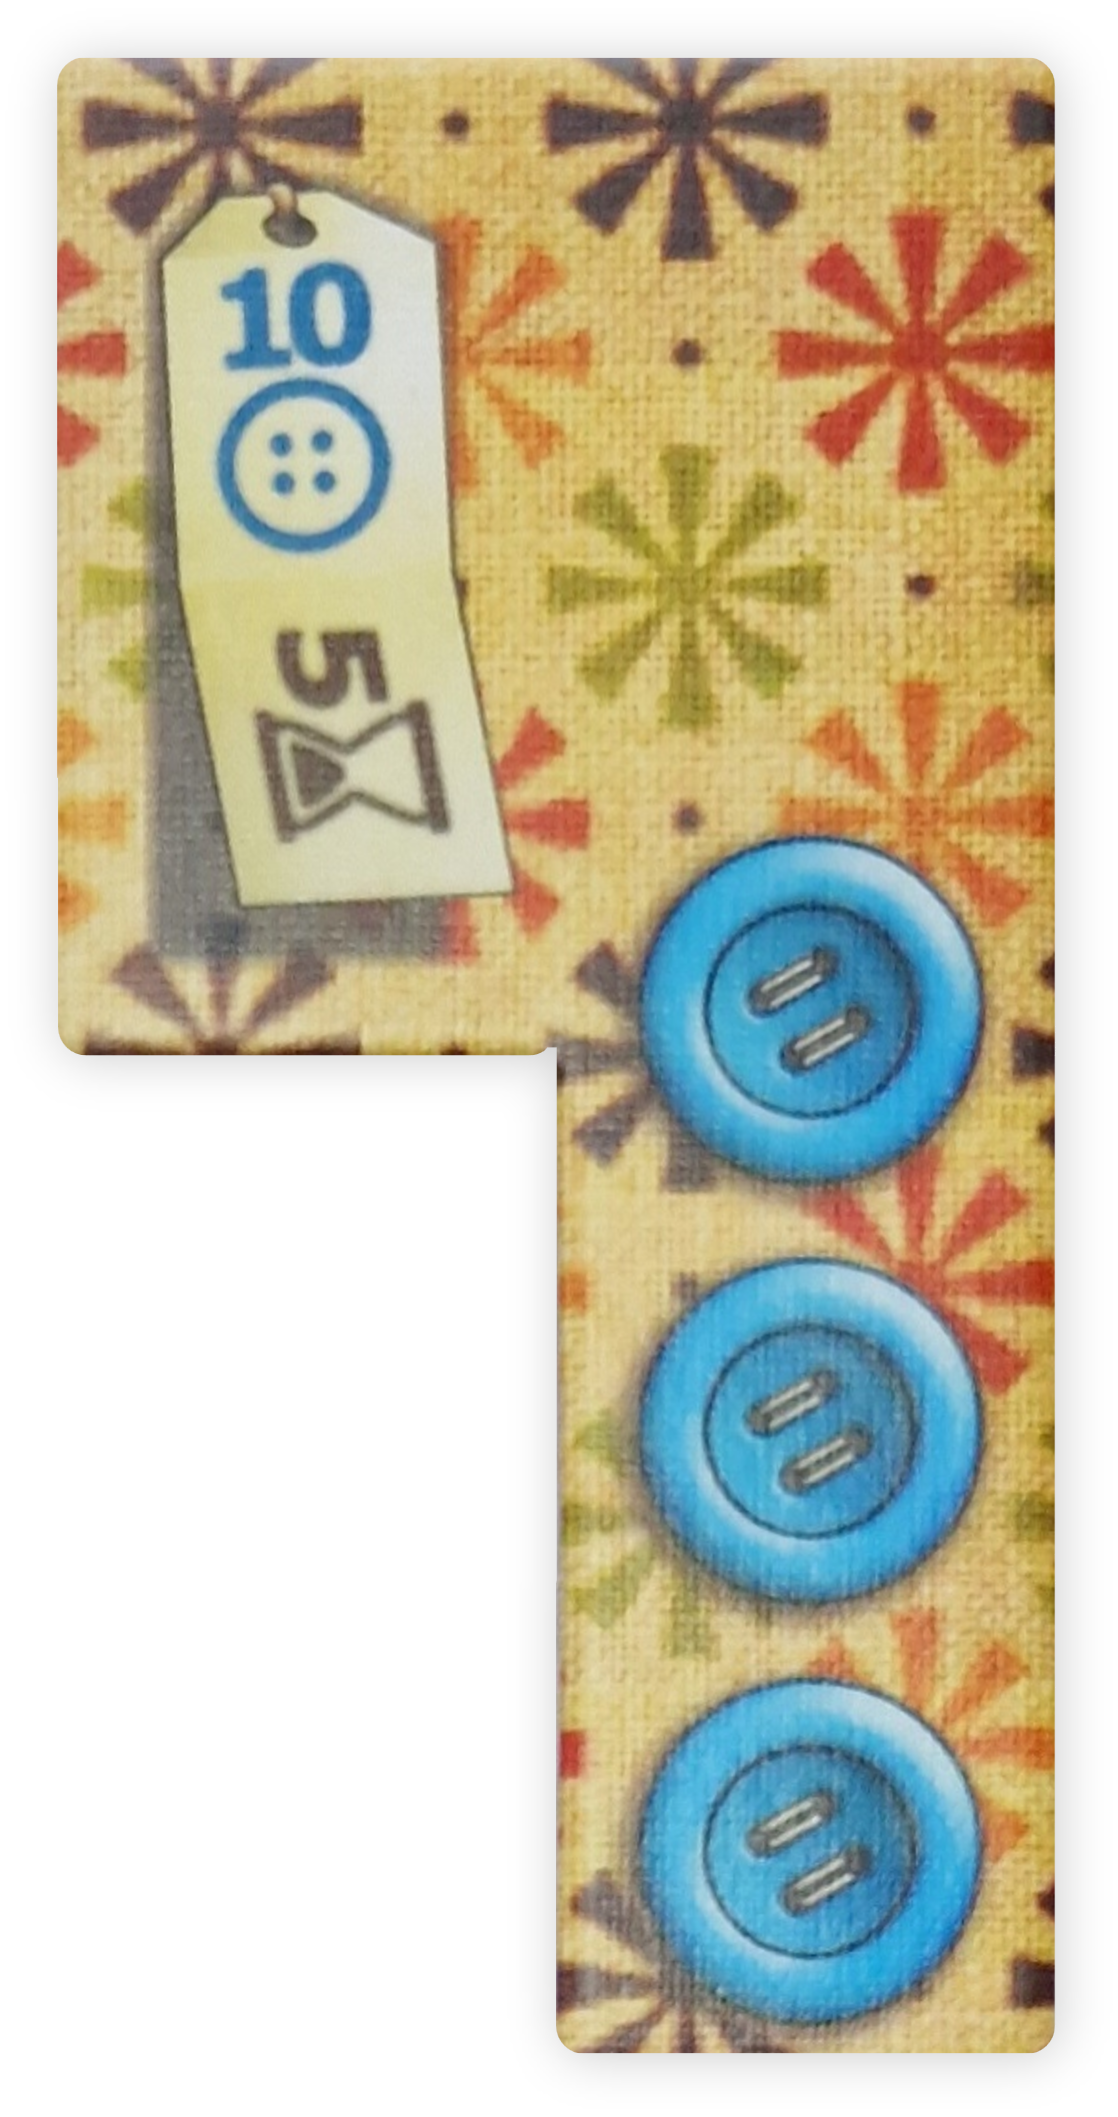
\includegraphics[width=0.2\textwidth]{res/pictures/assets/13-front.png}} & $13$ & $6$    & $7$              & $2$ & $2$ & $\frac{1}{16} \approx 0{,}167$ \\ \hline
    \adjustbox{valign=m, max width=0.2\textwidth, max height=0.1\textheight}{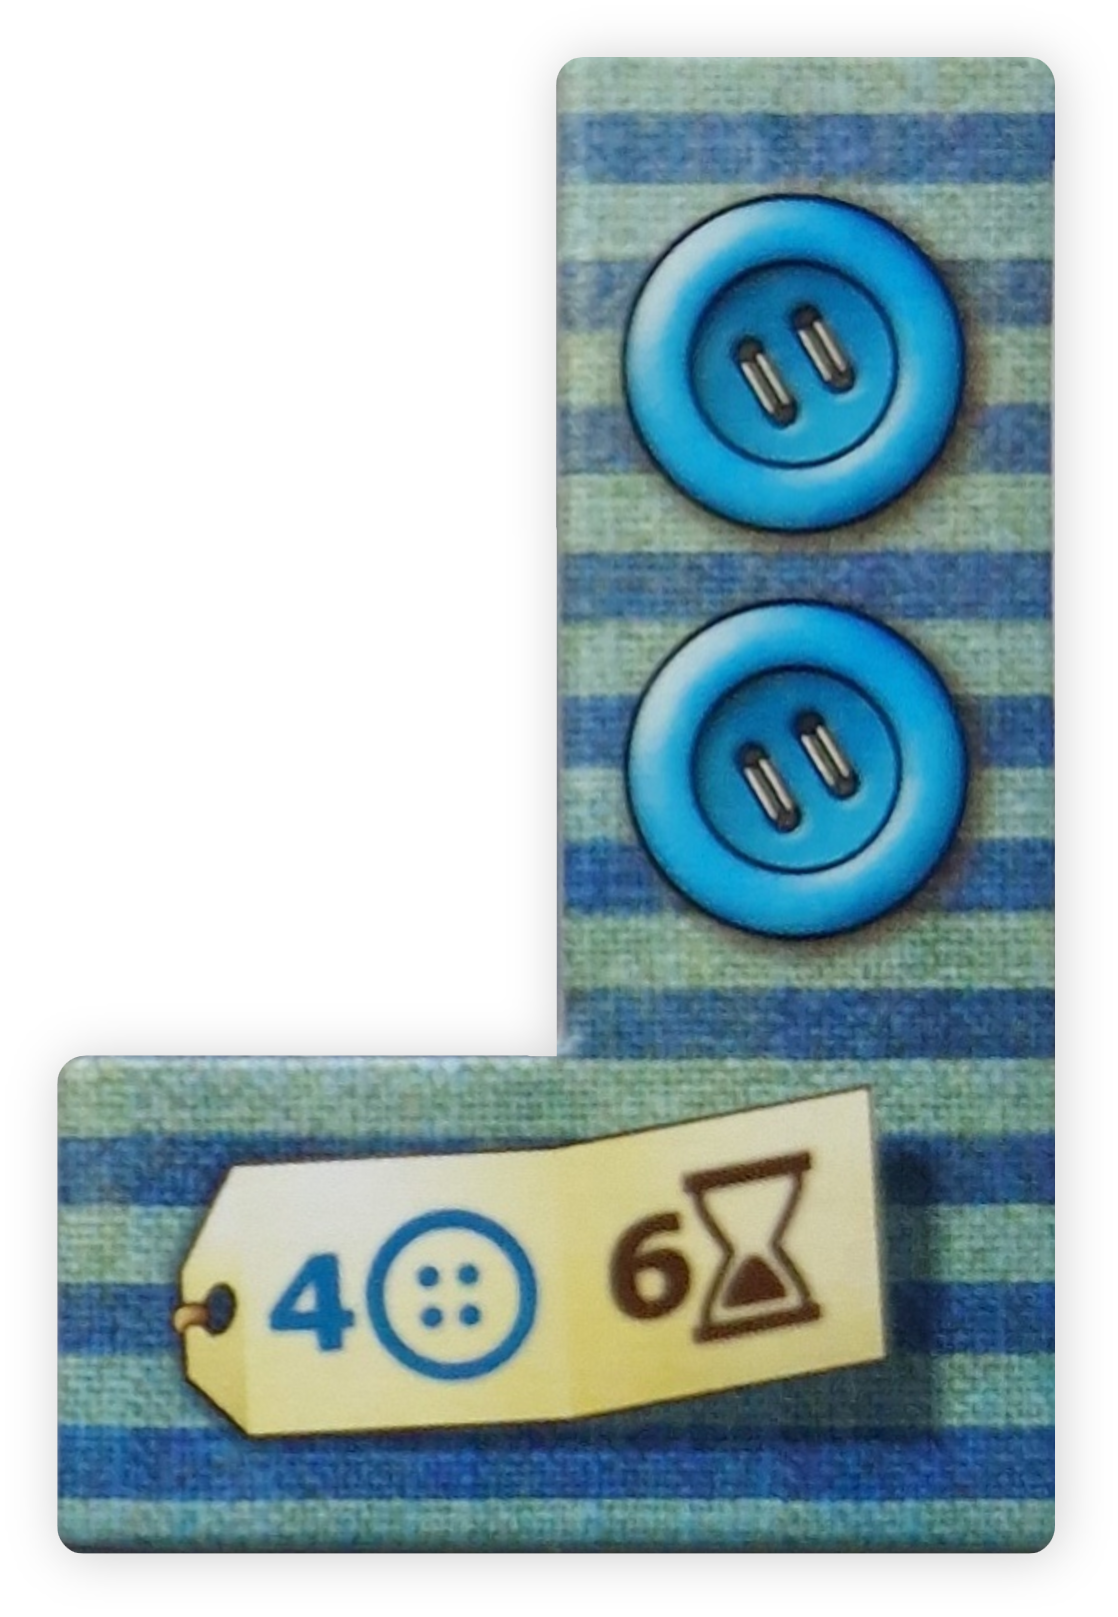
\includegraphics[width=0.2\textwidth]{res/pictures/assets/14-front.png}} & $14$ & $4$    & $4$              & $6$ & $2$ & $\frac{1}{12} \approx 0{,}083$ \\ \hline
    \adjustbox{valign=m, max width=0.2\textwidth, max height=0.1\textheight}{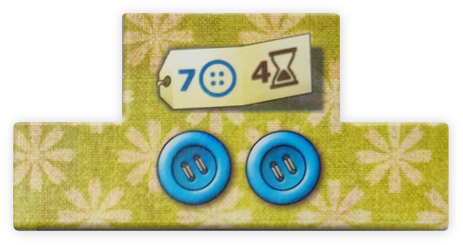
\includegraphics[width=0.2\textwidth]{res/pictures/assets/15-front.png}} & $15$ & $6$    & $7$              & $4$ & $2$ & $\frac{1}{12} \approx 0{,}083$ \\ \hline
    \adjustbox{valign=m, max width=0.2\textwidth, max height=0.1\textheight}{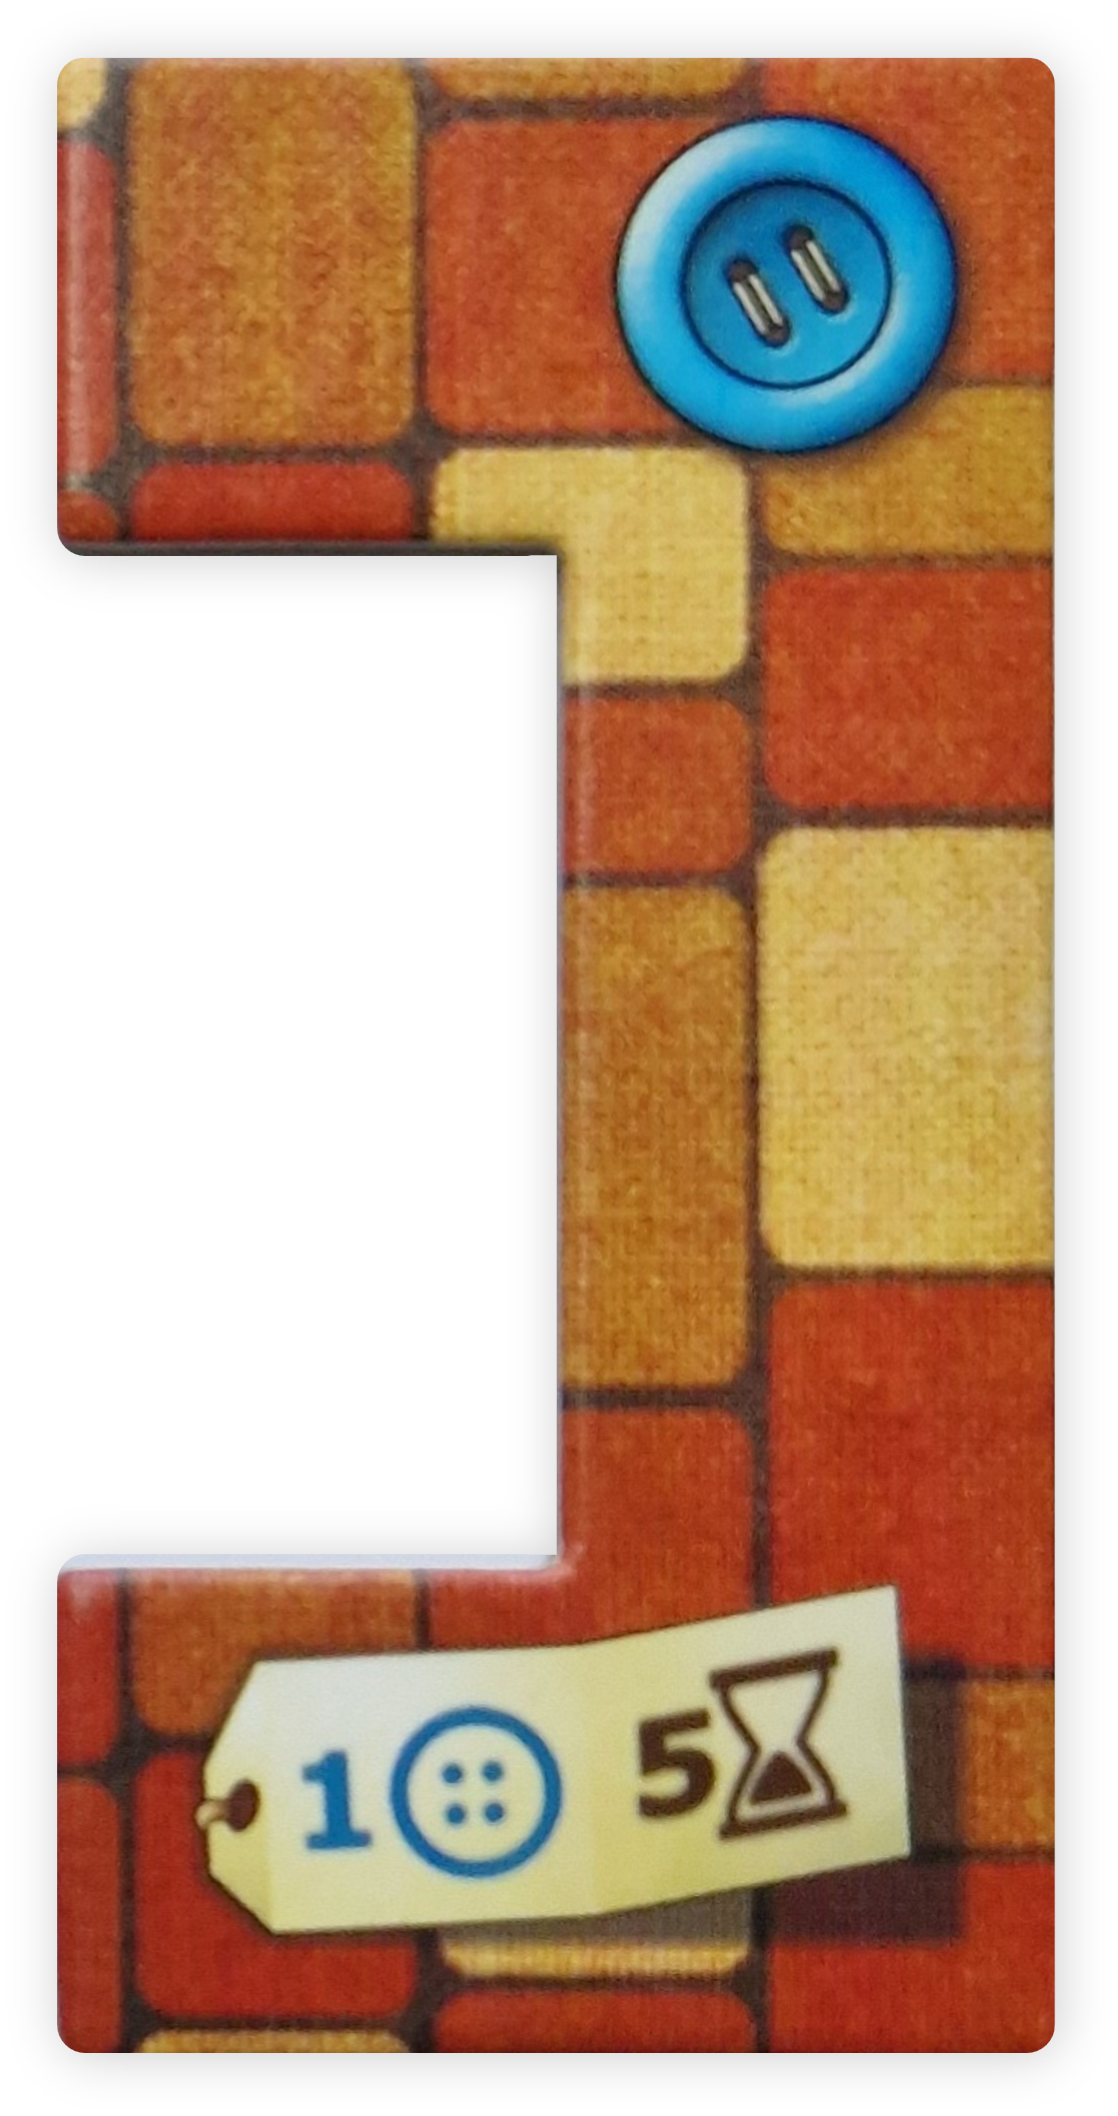
\includegraphics[width=0.2\textwidth]{res/pictures/assets/16-front.png}} & $16$ & $6$    & $1$              & $5$ & $1$ & $\frac{1}{30} \approx 0{,}033$ \\ \hline
    \adjustbox{valign=m, max width=0.2\textwidth, max height=0.1\textheight}{\includegraphics[width=0.2\textwidth]{res/pictures/assets/17-front.png}} & $17$ & $5$    & $5$              & $4$ & $2$ & $\frac{1}{10} = 0{,}1$         \\ \hline
    \adjustbox{valign=m, max width=0.2\textwidth, max height=0.1\textheight}{\includegraphics[width=0.2\textwidth]{res/pictures/assets/18-front.png}} & $18$ & $5$    & $10$             & $3$ & $2$ & $\frac{2}{15} \approx 0{,}133$ \\ \hline
    \adjustbox{valign=m, max width=0.2\textwidth, max height=0.1\textheight}{\includegraphics[width=0.2\textwidth]{res/pictures/assets/19-front.png}} & $19$ & $4$    & $4$              & $2$ & $1$ & $\frac{1}{8} = 0{,}125$        \\ \hline
    \adjustbox{valign=m, max width=0.2\textwidth, max height=0.1\textheight}{\includegraphics[width=0.2\textwidth]{res/pictures/assets/20-front.png}} & $20$ & $7$    & $1$              & $4$ & $1$ & $\frac{1}{28} \approx 0{,}036$ \\ \hline
    \adjustbox{valign=m, max width=0.2\textwidth, max height=0.1\textheight}{\includegraphics[width=0.2\textwidth]{res/pictures/assets/21-front.png}} & $21$ & $3$    & $1$              & $3$ & $0$ & $0$                            \\ \hline
    \adjustbox{valign=m, max width=0.2\textwidth, max height=0.1\textheight}{\includegraphics[width=0.2\textwidth]{res/pictures/assets/22-front.png}} & $22$ & $5$    & $1$              & $2$ & $0$ & $0$                            \\ \hline
    \adjustbox{valign=m, max width=0.2\textwidth, max height=0.1\textheight}{\includegraphics[width=0.2\textwidth]{res/pictures/assets/23-front.png}} & $23$ & $3$    & $3$              & $1$ & $0$ & $0$                            \\ \hline
    \adjustbox{valign=m, max width=0.2\textwidth, max height=0.1\textheight}{\includegraphics[width=0.2\textwidth]{res/pictures/assets/24-front.png}} & $24$ & $4$    & $2$              & $2$ & $0$ & $0$                            \\ \hline
    \adjustbox{valign=m, max width=0.2\textwidth, max height=0.1\textheight}{\includegraphics[width=0.2\textwidth]{res/pictures/assets/25-front.png}} & $25$ & $3$    & $2$              & $2$ & $0$ & $0$                            \\ \hline
    \adjustbox{valign=m, max width=0.2\textwidth, max height=0.1\textheight}{\includegraphics[width=0.2\textwidth]{res/pictures/assets/26-front.png}} & $26$ & $4$    & $3$              & $2$ & $1$ & $\frac{1}{8} = 0{,}125$        \\ \hline
    \adjustbox{valign=m, max width=0.2\textwidth, max height=0.1\textheight}{\includegraphics[width=0.2\textwidth]{res/pictures/assets/27-front.png}} & $27$ & $5$    & $7$              & $1$ & $1$ & $\frac{1}{5} = 0{,}2$          \\ \hline
    \adjustbox{valign=m, max width=0.2\textwidth, max height=0.1\textheight}{\includegraphics[width=0.2\textwidth]{res/pictures/assets/28-front.png}} & $28$ & $4$    & $3$              & $3$ & $1$ & $\frac{1}{12} \approx 0{,}083$ \\ \hline
    \adjustbox{valign=m, max width=0.2\textwidth, max height=0.1\textheight}{\includegraphics[width=0.2\textwidth]{res/pictures/assets/29-front.png}} & $29$ & $5$    & $5$              & $5$ & $2$ & $\frac{2}{25} = 0{,}08$        \\ \hline
    \adjustbox{valign=m, max width=0.2\textwidth, max height=0.1\textheight}{\includegraphics[width=0.2\textwidth]{res/pictures/assets/30-front.png}} & $30$ & $6$    & $3$              & $6$ & $2$ & $\frac{1}{18} \approx 0{,}056$ \\ \hline
    \adjustbox{valign=m, max width=0.2\textwidth, max height=0.1\textheight}{\includegraphics[width=0.2\textwidth]{res/pictures/assets/31-front.png}} & $31$ & $5$    & $3$              & $4$ & $1$ & $\frac{1}{20} = 0{,}05$        \\ \hline
    \adjustbox{valign=m, max width=0.2\textwidth, max height=0.1\textheight}{\includegraphics[width=0.2\textwidth]{res/pictures/assets/32-front.png}} & $32$ & $6$    & $0$              & $3$ & $1$ & $\frac{1}{18} \approx 0{,}056$ \\ \hline
\end{longtable}

% Reset to default
% \setlength{\tabcolsep}{6pt}

\newpage
\end{document}
